%-------------------------------------------------------------------
% Document class and package definitions
%-------------------------------------------------------------------
\documentclass[12pt,a4paper,openright,final,twoside]{msethesis}
%Included for Gather Purpose only:
%input "thesisreferences.bib"

\usepackage{epigraph}

\addbibresource{thesisreferences.bib}
\addbibresource{paperA/refspaperA.bib}

\begin{document}

\newrefsection

%\defaultbibliography{thesisreferences}     %% Change this only.
%\defaultbibliographystyle{ieeetr}        %% Could be changed if you like
                                           %% references typeset differently.
%-------------------------------------------------------------------
% Define title, author, etc.
%-------------------------------------------------------------------
\def\thesistitle{Influence of microstructure on debonding at the fiber/matrix interface in fiber-reinforced polymers under tensile loading}
\def\theauthor{Luca Di Stasio}
\def\theaddress{Division of Materials Science\\Department of Engineering Sciences and Mathematics\\
Lule{\aa} University of Technology\\ Lule{\aa}, Sweden}

\def\supervisors{Janis Varna, Zoubir Ayadi}
\def\supervisorstring{Supervisors:} % Edit here if you have only one supervisor
\def\dedication{A mio figlio, Levante Libero Antonio}

% Read abstract and preface from separate files.
% Make sure these exist. See example files.
\def\theabstract{At the end of the second decade of the XXI century, the transportation industry at large faces several challenges that will shape its evolution in the next decade and beyond. The first main challenge is the increasing public awareness and governmental action on climate change, which are increasing the pressure on the industrial sectors responsible for the greatest share of emissions, the transportation industry being one of them, to reduce their environmental footprint. A second challenge lies instead in the renewed push toward price reduction, due to increased competition (as for example the entry of private entities in the market for low-Earth orbit launchers) and innovative business models (like ride-sharing and ride-hailing in the automotive sector or low-cost carriers in civil aviation).\\
A common technical solution strategy to these challenges is the reduction of vehicles' structural mass, while keeping the payload mass constant. By reducing consumption, a reduced weight leads to reduced emissions in fossil-fuels powered vehicles and to increased autonomy in electrical vehicles. By reducing the quantity of materials required in structures, a weight reduction strategy favors a reduction of production costs and thus lower prices. Transportation is however a sector where safety is a paramount concern, and structures must satisfy strict requirements and validation procedures to guarantee their integrity and reliability during service life. This represents a significant constraint which limits the scope of weight reduction strategies.\\
In the last twenty years, the development of a novel type of Fiber-Reinforced Polymer Composite (FRPC) laminates, i.e. \emph{thin-ply} laminates, proposes a solution to these competing requirements (weight with to respect to structural integrity) by providing at the same time weight reduction and increased strength. Several experimental investigations have shown, in fact, that \emph{thin-ply} laminates are capable of delaying, and even suppress, the onset of transverse cracking. Transverse cracks are a kind of sub-critical damage and occur early in the failure process, causing the degradation of elastic properties and favoring other, often more critical, modes of damage (delaminations, fiber breaks). Delay and suppression of transverse cracks were already linked, at the of the 1970's, to the use of thinner plies. However, \emph{thin-plies} available today on the market are at least 10 times thinner than those studied in the 1970's. This changes the length scale of the problem, from millimeters to micrometers. At the microscale, transverse cracks are formed by several fiber/matrix interface cracks (or debonds) coalescing together. Understanding the mechanisms of transverse cracking delay and suppression in \emph{thin-ply} laminates implies 
}
\def\thepreface{I bought my first and current car, \emph{La Melanza}, in August 2015, just a few weeks before starting my doctoral studies at Lule\aa\ University of Technology and Universit\'e de Lorraine. Today, October 2019, emph{La Melanza} has traveled kilometers. It has been, indeed, a long journey. One that has brought me to live in two different countries, France and Sweden, and to visit five more, Germany, Greece, Russia, Italy and Spain, for conferences, summer schools and exchanges. A journey in which I have learned a lot, made new friends and built a family. And, apparently, even managed to write a Ph.D. thesis! No such journey could be ventured alone, and here I would like to thank everyone who helped and supported me in these years.\\
It is common use to place supervisors at the top of the acknowledgements list, and I will not be any different. It is however not in adherence to custom, but with sincere gratitude that I place them here in the first place. Thus, many thanks to Prof. Janis Varna for accepting me as his Ph.D. student, sharing his knowledge, correcting my mistakes, pointing my efforts in the right direction, always being curious and passionate about research. Thanks to Prof. Zoubir Ayadi, for welcoming me in France and supporting me all along.\\
I then wish to thank all the members of Polymeric Composite Group at LTU for welcoming me in Lule\aa, for showing me how to survive at $-30^{\circ}$, for the interesting discussions over a coffee and for their help to solve the problems in the lab: Johanna, Roberts, Patrik, Lennart, Zainab, Nawres, Hiba, Liva, Andrejs, Linqi.\\
I wish to thank also all the people that have helped me extricate myself in all the administrative needs that an international project requires, and have always answered with patience and a smile to my (at times many) questions: Birgitta, Fredrik, Marie-Louise, Christine, Martine, Nadine and Flavio.\\
And finally, my thoughts go to my family. To Scarlett, for ``the purest love in the world is between a grumpy dad and the pet he said he never wanted", and I guess I'm just another proof of it. To Levante, for forcing me to work to stay awake late at night guarding him, and for bringing already so much joy in my life. To Valentina, for following me in two different countries, for bringing so many beautiful things in my life and, every now and then, reminding me that there are worse things in life than a deadline for a paper (or a thesis!).\\

\noindent Lule\aa, October 2019\\
Luca Di Stasio
}


% Change here if you want to remove the logo printed on the first page

%\def\thelogo{
\includegraphics[width=2.5cm]{eu1_f_eng}} % old EU logo
\def\thelogo{} % no logo

% The definitions above could be put directly in the function call below,
% but is here defined explicitly, for the purpose of clarity.

\startpreamble
  {\thesistitle}
  {\theauthor}
  {\theaddress}
  {\supervisors}
  {\dedication}
  {\theabstract}
  {\thepreface}
  {\thelogo}

%%%%%%%%%%%%%%%%%%%%%%%%%%%%%%%%%%%%%%%%%%%%%%%%%%%%%%%%%%%%%%%%%%%%
%% Begin Part I
%%%%%%%%%%%%%%%%%%%%%%%%%%%%%%%%%%%%%%%%%%%%%%%%%%%%%%%%%%%%%%%%%%%%
\makepartpage{Part I}

%% Initialize part containing the thesis introduction chapters
\startchapters

%\begin{bibunit}
%------------------------ Start chapter 1 --------------------------
% The \makechapter command takes three arguments
%  1) An abbreviated version of the chapter name,
%     to be used as page header
%  2) String to be added to the table of contents
%  3) The chapter name, possibly split in to lines,
%     as in Chapter 2 below.
%
%  The different arguments can have different line breaks.
%
% The actual contents of the chapter is included by removing the
% comment from the \input line below. Make sure the file
% chapter1.tex exists.
%-------------------------------------------------------------------

%\def\myquote{``This report, by its very length, defends itself against the risk of being read."\\[.5\baselineskip] Winston Churchill}

%\makechapter{Running header}{Table of contents entry}{Title
%appearing on the\\ chapter start page\label{ch2}}
%\section{The World Wide Failure Exercises}
This is the text of the second chapter. \cite{*}

\appendix
\section{This is an appendix section}
Text of the appendix

\subsection{Subsection 1}
Yet some text, and an equation
\begin{equation}
    \textnormal{abs}\left(e^{j\pi}\right)=\,?
\end{equation}

\subsection{Subsection 2}
And then some...

\section{This is another appendix section}
This section concludes the appendix.


\def\chaponequote{\dots a ``sage", as an anonymous writer has pointed out, ``calls up in the average mind the picture of something grey and pedantic if not green and aromatic"\\[.5\baselineskip]Arthur D. Little}
\def\chaponequotetext{\dots a ``sage", as an anonymous writer has pointed out, ``calls up in the average mind the picture of something grey and pedantic if not green and aromatic".}
\def\chaponequoteauthor{Arthur D. Little~\cite{Little1924}}
\makechapter{A journey of scales}{A journey of scales}{A journey of scales\label{ch1}}
\epigraph{\chaponequotetext}{\chaponequoteauthor}
%%%%%%%%%%%%%%%%%%%%%%%%%%%%%%%%%%%%%%%%%%%%%%%%%%%%%%%%%%%%%%%%%%%%%%%
%      SEC. 1
%%%%%%%%%%%%%%%%%%%%%%%%%%%%%%%%%%%%%%%%%%%%%%%%%%%%%%%%%%%%%%%%%%%%%%%
\section{Introduction and structure of the thesis}

Passion and curiosity should always lie at the heart of the scientific practice, and that ought to be enough to define the value of a research effort~\cite{Weber1917,Shapin2015}. Time is the real arbiter of the significance of a piece of research, as many examples in the history of science show~\cite{Brush1967,Niss2008}\footnote{The Ising-Lenz model is one such example~\cite{Brush1967,Niss2008,Niss2004}. It was suggested by physicist Wilhelm Lenz to his doctoral student Ernst Ising to study phase transitions in ferromagnetic materials. Ising solved it analytically in 1D as part of his Ph.D. defense in 1925, but the solution for a 1D lattice did not show any phase transition. This apparent failure is thought to be the reason of Ising's decision to take a job outside academia. Almost 20 years later, Onsager solved the 2D version of the model and showed the possibility of phase transitions in the Ising-Lenz model. By the time Ising arrived in the USA in 1947, the Ising-Lenz model was already entering the canon of physics and, to his surprise, he was being asked if he was ``the Ising" of the ``Ising model".}.However, in these years of increasing mistrust towards scientific research and brewing doubts on the value of universities and research institutes~\cite{Biesta2002,Biesta2004,Santos2012}, it is worthwhile to try to place one's own work into the wider picture of one's own time. It is also a valuable exercise for the researcher, who sensibly progresses in the work by investigating one detail at a time, to spend a moment away from one's own graphs and equations and see their place in the wider perspective of the world outside the laboratory.\\
It is thus in this spirit that I propose to open the present work with a reflection on the challenges that the transportation industry faces at the closing of $21^{st}$ century's second decade. Against this background, in Chapter~1 \emph{thin-ply} laminates are introduced as a very promising material for innovative structural design and their main characteristics are discussed. The focus is then moved to the most renown quality of \emph{thin-ply} laminates, i.e. their ability to delay and even suppress onset and propagation of transverse cracking, and to discuss the modeling issues that this new material poses. Finally, a link is established with the growth of fiber/matrix interface cracks or, as very often called in the rest of the thesis, debonds. Chapter~2 opens with an introduction to the main concepts of Fracture Mechanics. The fiber/matrix interface crack is then discussed in detail, and previous analytical, computational and experimental studies available in the literature are reviewed. The modeling strategy adopted in this thesis is then presented and its implementation described. Finally, Chapter~3 provides a summary of the main results of this work, organized following the order of the publications reported in Part~II of the thesis. The first chapter is thus a journey of scales: we start from the challenges of an industrial sector, move to the structural requirements of its products, focus on a promising new material, and concentrate on understanding the mechanisms of damage initiation in it.

\section{Vision 2030: challenges of the next decade and beyond for the transportation industry}

The closing of the second decade of the $21^{st}$ century brings different challenges for the transportation industry, which will likely shape its development in the next decade and beyond. A brief review of the most relevant aspects is proposed here.

\begin{description}
\item[Climate action.] The issue of climate change is certainly one the ``hot" topic of today's public debate. A discussion of the merits of scientific understanding of climate change, public reception, media coverage and socio-political implications is out of the scope of the present work, but it is certainly one of the most relevant topic framing today's public discourse. Given that it is a high-divisive subject, no judgement on the validity of the claims of one side or the other is proposed here, as sufficient space can not be devoted to a thorough analysis of the problem. What is acknowledged here is the emergence of concerted efforts at the institutional level (companies, city administrations, regional governments, sovereign states) to rule into and provide control mechanisms to limit the emission of carbon dioxide, i.e. $CO_{2}$. Some relevant data is also presented in order to show the importance of the issue for the transportation industry.

\begin{figure}
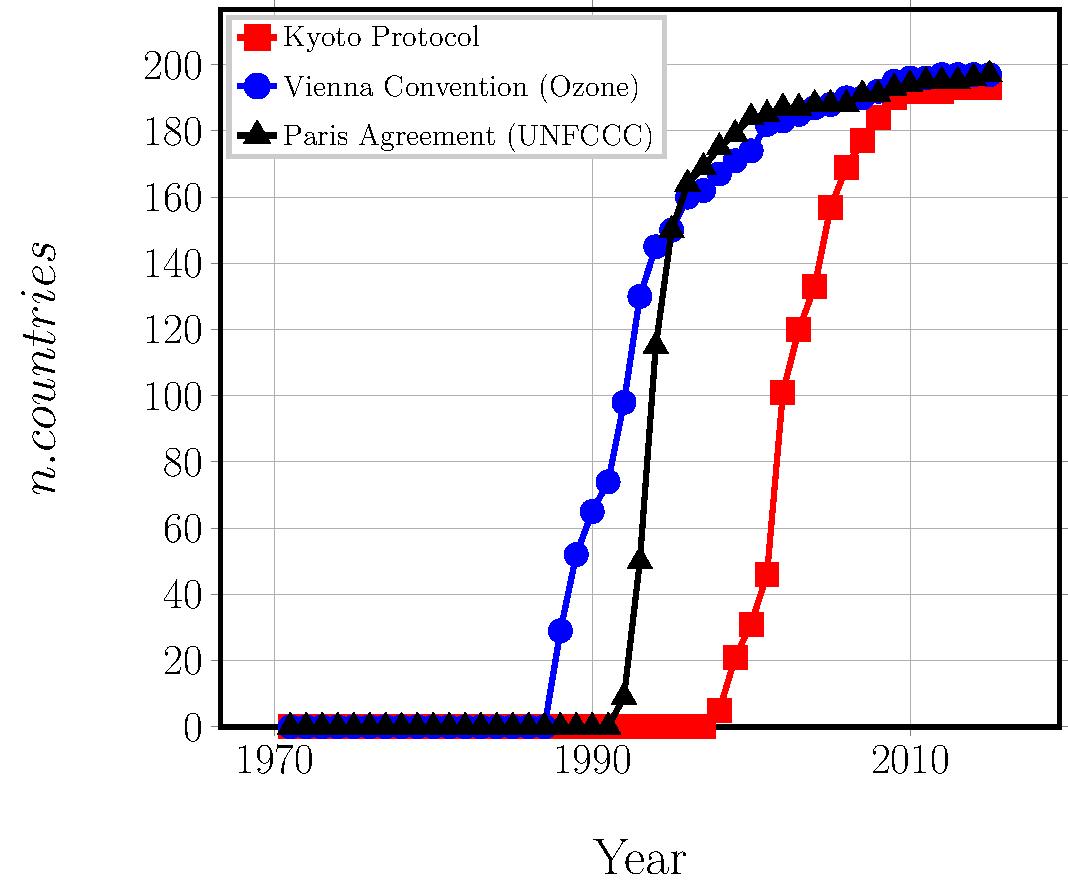
\includegraphics[width=\textwidth]{climate-deals-signataries.pdf}
\caption{Number of signing countries over time for selected deals on climate.}\label{chap1:fig:climatedealssignataries}
\end{figure}

\begin{figure}
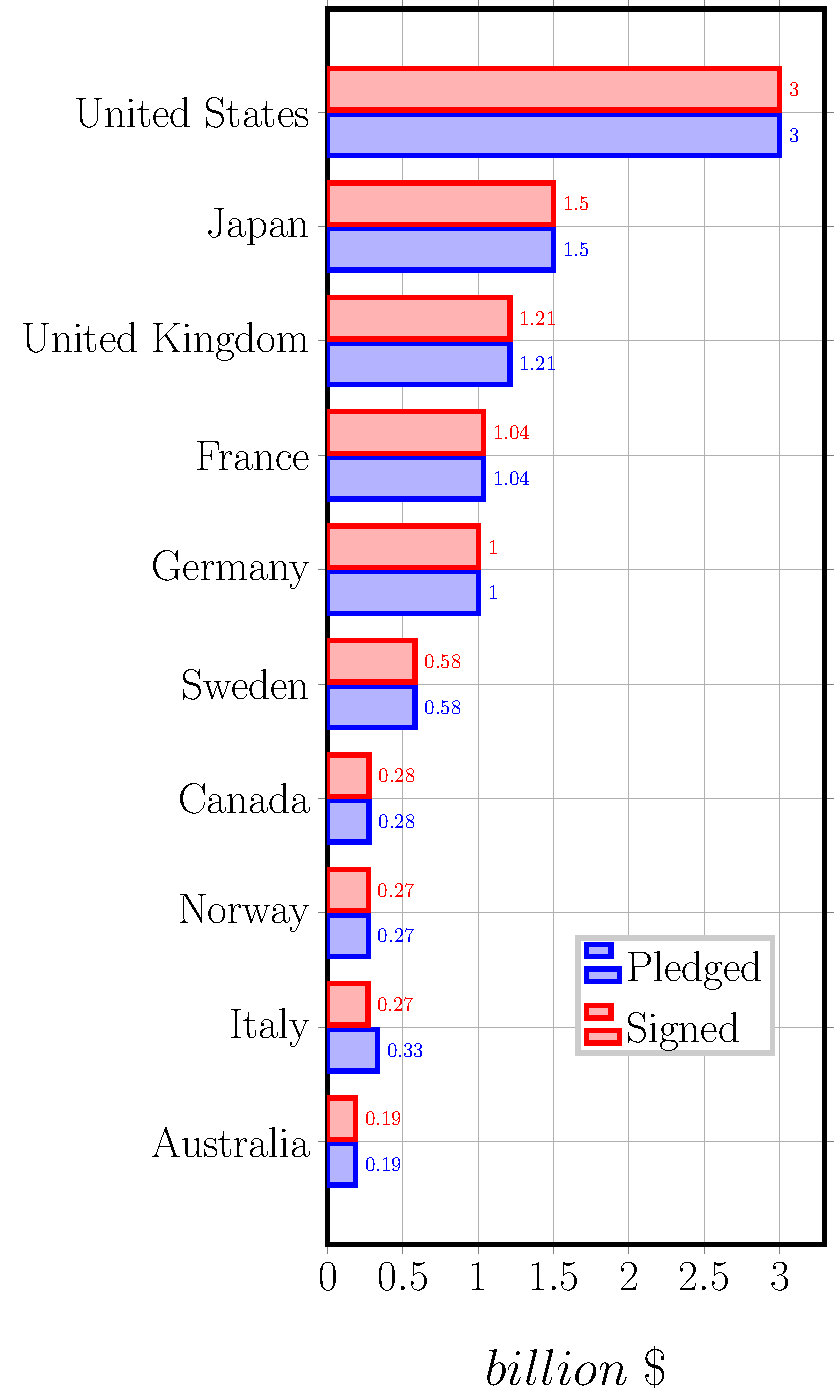
\includegraphics[width=\textwidth]{green-fund-pledges.pdf}
\caption{Pledges to the Green Climate Fund for selected countries.}\label{chap1:fig:greenfundpledges}
\end{figure}

\begin{figure}
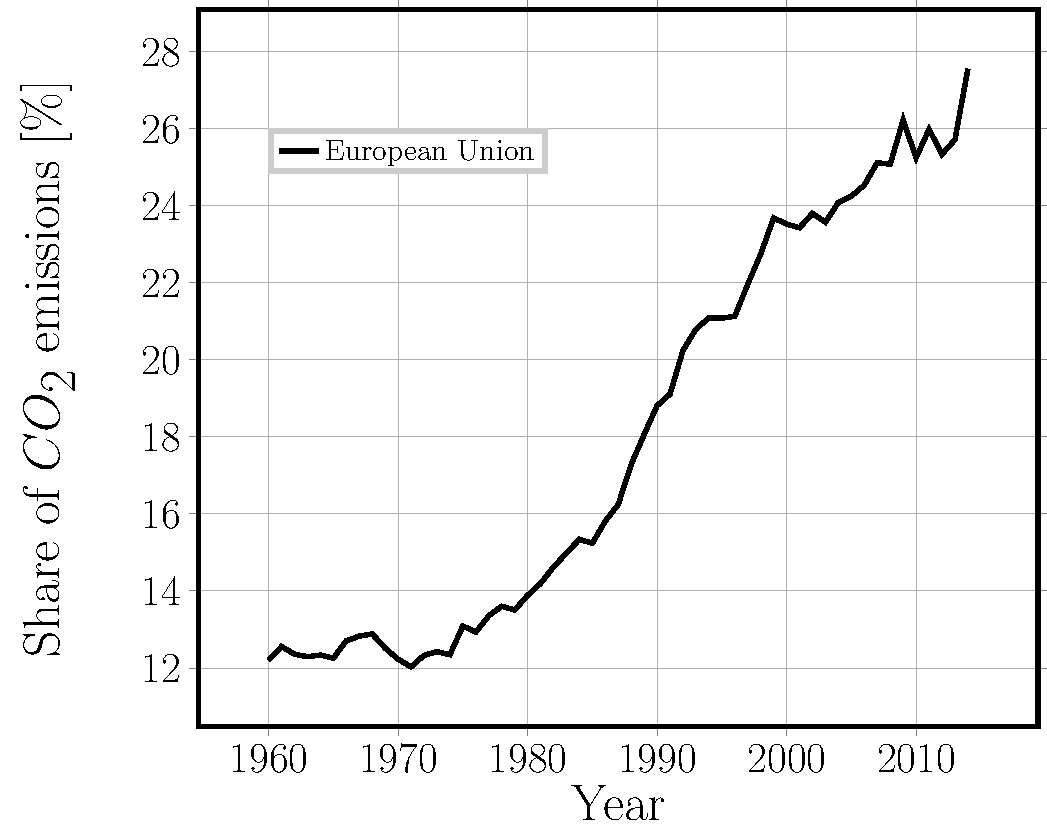
\includegraphics[width=\textwidth]{co2transportshare.pdf}
\caption{Pledges to the Green Climate Fund for selected countries.}\label{chap1:fig:co2transportshare}
\end{figure}

\begin{figure}
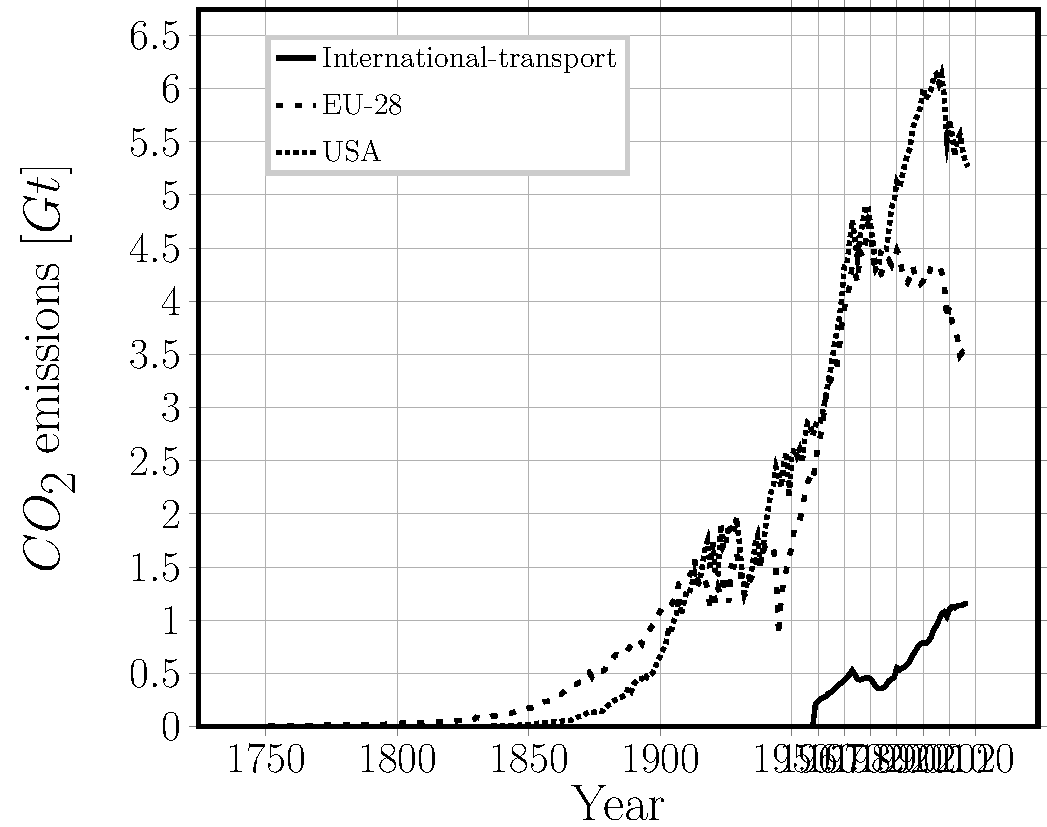
\includegraphics[width=\textwidth]{co2transportabsolute.pdf}
\caption{Pledges to the Green Climate Fund for selected countries.}\label{chap1:fig:co2transportabsolute}
\end{figure}

\end{description}


\makechapter{Modeling damage in FRPC}{Modeling damage in FRPC}{Modeling damage in FRPC}
%\section{The World Wide Failure Exercises}
This is the text of the second chapter. \cite{*}

\appendix
\section{This is an appendix section}
Text of the appendix

\subsection{Subsection 1}
Yet some text, and an equation
\begin{equation}
    \textnormal{abs}\left(e^{j\pi}\right)=\,?
\end{equation}

\subsection{Subsection 2}
And then some...

\section{This is another appendix section}
This section concludes the appendix.


\makechapter{The fiber-matrix interface crack problem}{The fiber-matrix interface crack problem}{The fiber-matrix interface crack problem}
%%%%%%%%%%%%%%%%%%%%%%%%%%%%%%%%%%%%%%%%%%%%%%%%%%%%%%%%%%%%%%%%%%%%%%%%
%      Paper A
%%%%%%%%%%%%%%%%%%%%%%%%%%%%%%%%%%%%%%%%%%%%%%%%%%%%%%%%%%%%%%%%%%%%%%%
\section{Paper A}
\section*{Finite Element solution of the fiber/matrix interface crack problem: convergence properties and mode mixity of the Virtual Crack Closure Technique}

The analysis of bi-material interface cracks, such as the fiber/matrix interface crack or debond, in the context of Linear Elastic Fracture Mechanics hides some peculiar complexities due to the nature of the solution at the crack tip. The solution to the fiber/matrix interface crack problem can be classified into two different regimes~\cite{Paris1996,Varna1997a}: the \emph{open crack} and \emph{closed crack} solution. The distinction between the two lies in the existence of a region of contact between crack faces (contact zone) at the crack tip: if it exists, we talk about a \emph{closed crack} solution, otherwise of an \emph{open crack} solution.\\
The \emph{open crack} solution to the straight bi-material interface crack problem was first proposed by Williams~\cite{Williams1959}, who found the existence of an oscillatory singularity in the stress field at the crack tip of the form

\begin{equation}\label{chap3:paperA:eq:singularitywilliams}
r^{-\frac{1}{2}}\sin\left(\varepsilon\log r\right)\quad\text{with}\quad\varepsilon=\frac{1}{2\pi}\log\left(\frac{1-\beta}{1+\beta}\right),
\end{equation}

in both Mode I and Mode II. In Eq.~\ref{chap3:paperA:eq:singularitywilliams}, $\beta$ is one of the two parameters introduced by Dundurs~\cite{Dundurs1969} to characterize bi-material interfaces:

\begin{equation}\label{chap3:paperA:eq:dundursbeta}
\beta=\frac{\mu_{2}\left(\kappa_{1}-1\right)-\mu_{1}\left(\kappa_{2}-1\right)}{\mu_{2}\left(\kappa_{1}+1\right)+\mu_{1}\left(\kappa_{2}+1\right)}
\end{equation}

where $\kappa=3-4\nu$ in plane strain and $\kappa=\frac{3-4\nu}{1+\nu}$ in plane stress, $\mu$ is the shear modulus, $\nu$ Poisson's coefficient, and indexes $1,2$ refer to the two bulk materials joined at the interface. Due to the nature of singular solution at the crack tip in the \emph{open crack} case, the definition of Stress Intensity Factor (SIF) $\lim_{r\rightarrow 0}\sqrt{2\pi r}\sigma$ diverges and is not anymore valid~\cite{Comninou1990}. The mismatch in the value of the elastic properties at the bi-material interface makes the configuration a mixed-mode one, but the Mode mixity problem at the crack tip is ill-posed. For the same reason, Mode I and Mode II Energy Release Rate do not converge. A way to circumvent the problem is to evaluate the ERR over a finite instead of an infinitesimal crack increment, which leads naturally to the application of the Virtual Crack Closure Technique (VCCT)~\cite{Rybicki1977,Krueger2004}.\\
The introduction of a finite crack increment makes the ERR sensitive to the mesh. Several authors have investigated the mesh sensitivity of the VCCT used in conjunction with the Finite Element Method (FEM) in the context of the straight bi-material interface crack~\cite{Krueger2013,Sun1987,Sun1989,Manoharan1990,Raju1988,Agrawal2006,Wang2013} and found that: the total Energy Release Rate $G_{TOT}$ does not depend on the mesh size; for a crack under mixed-mode behavior (\emph{open crack} case), Mode I and Mode II depend on the size of the mesh at the crack tip and do not show convergence. The purpose of this first paper is to analyze the mesh dependency of Energy Release Rate in the case of the fiber/matrix interface crack.

\begin{figure}[!h]
\centering
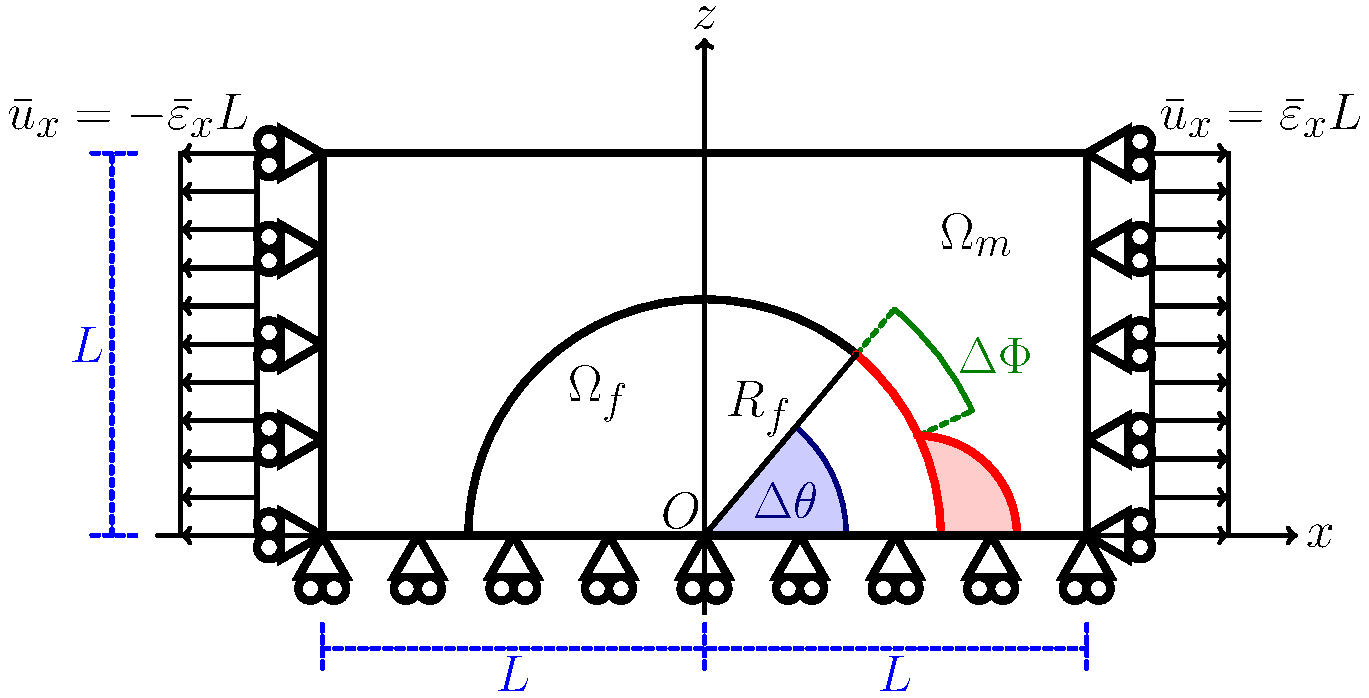
\includegraphics[width=\textwidth]{paperA/RUC.pdf}
\caption{Schematic of the model with its main parameters.}\label{chap3:paperA:fig:modelschem}
\end{figure}

The 1-step VCCT in the force-displacement formulation~\cite{Krueger2004} is considered and applied to the evaluation of the ERR of a debond located on a single fiber placed in a square matrix cell, as shown in Figure~\ref{chap3:paperA:fig:modelschem}. The cell has a size of $2L\times2L$, where

\begin{equation}\label{chap3:paperA:eq:LVf}
L=\frac{R_{f}}{2}\sqrt{\frac{\pi}{V_{f}}},
\end{equation}

$V_{f}$ is the fiber volume fraction and $R_{f}$ is the fiber radius, assumed to be equal to $1\ \mu m$. The occurrence of a contact zone after a critical size of the debond is considered and a contact pair interaction is established between crack faces. The interaction is considered frictionless. As the model is symmetric with respect to the $x$-axis (see Figure~\ref{chap3:paperA:fig:modelschem}), only half of it is explicitly modeled and symmetry conditions are applied to the lower boundary. A constant $x$-strain of $1\%$ is applied to the right and left boundary. Glass fiber and epoxy are considered and their properties are reported in Table~\ref{chap3:paperA:tab:phaseprop}.

\begin{table}[!htbp]
 \centering
 \caption{Summary of the mechanical properties of fiber and matrix. $E$ stands for Young's modulus, $\mu$ for shear modulus and $\nu$ for Poisson's ratio.}
 \begin{tabular}{cccc}
\textbf{Material} & \textbf{$E\left[GPa\right]$}\ & \textbf{$\mu\left[GPa\right]$} & \textbf{$\nu\left[-\right]$} \\
\midrule
Glass fiber    & 70.0  & 29.2   & 0.2  \\
Epoxy    & 3.5    & 1.25   & 0.4
\end{tabular}
\label{chap3:paperA:tab:phaseprop}
\end{table}

The main parameter of the mesh sensitivity study is the angular size $\delta$ of the elements at the crack tip, as shown in Figure~\ref{chap3:paperA:fig:vcctmesh}.

\begin{figure}[!h]
\centering
    \begin{subfigure}[b]{0.8\textwidth}
        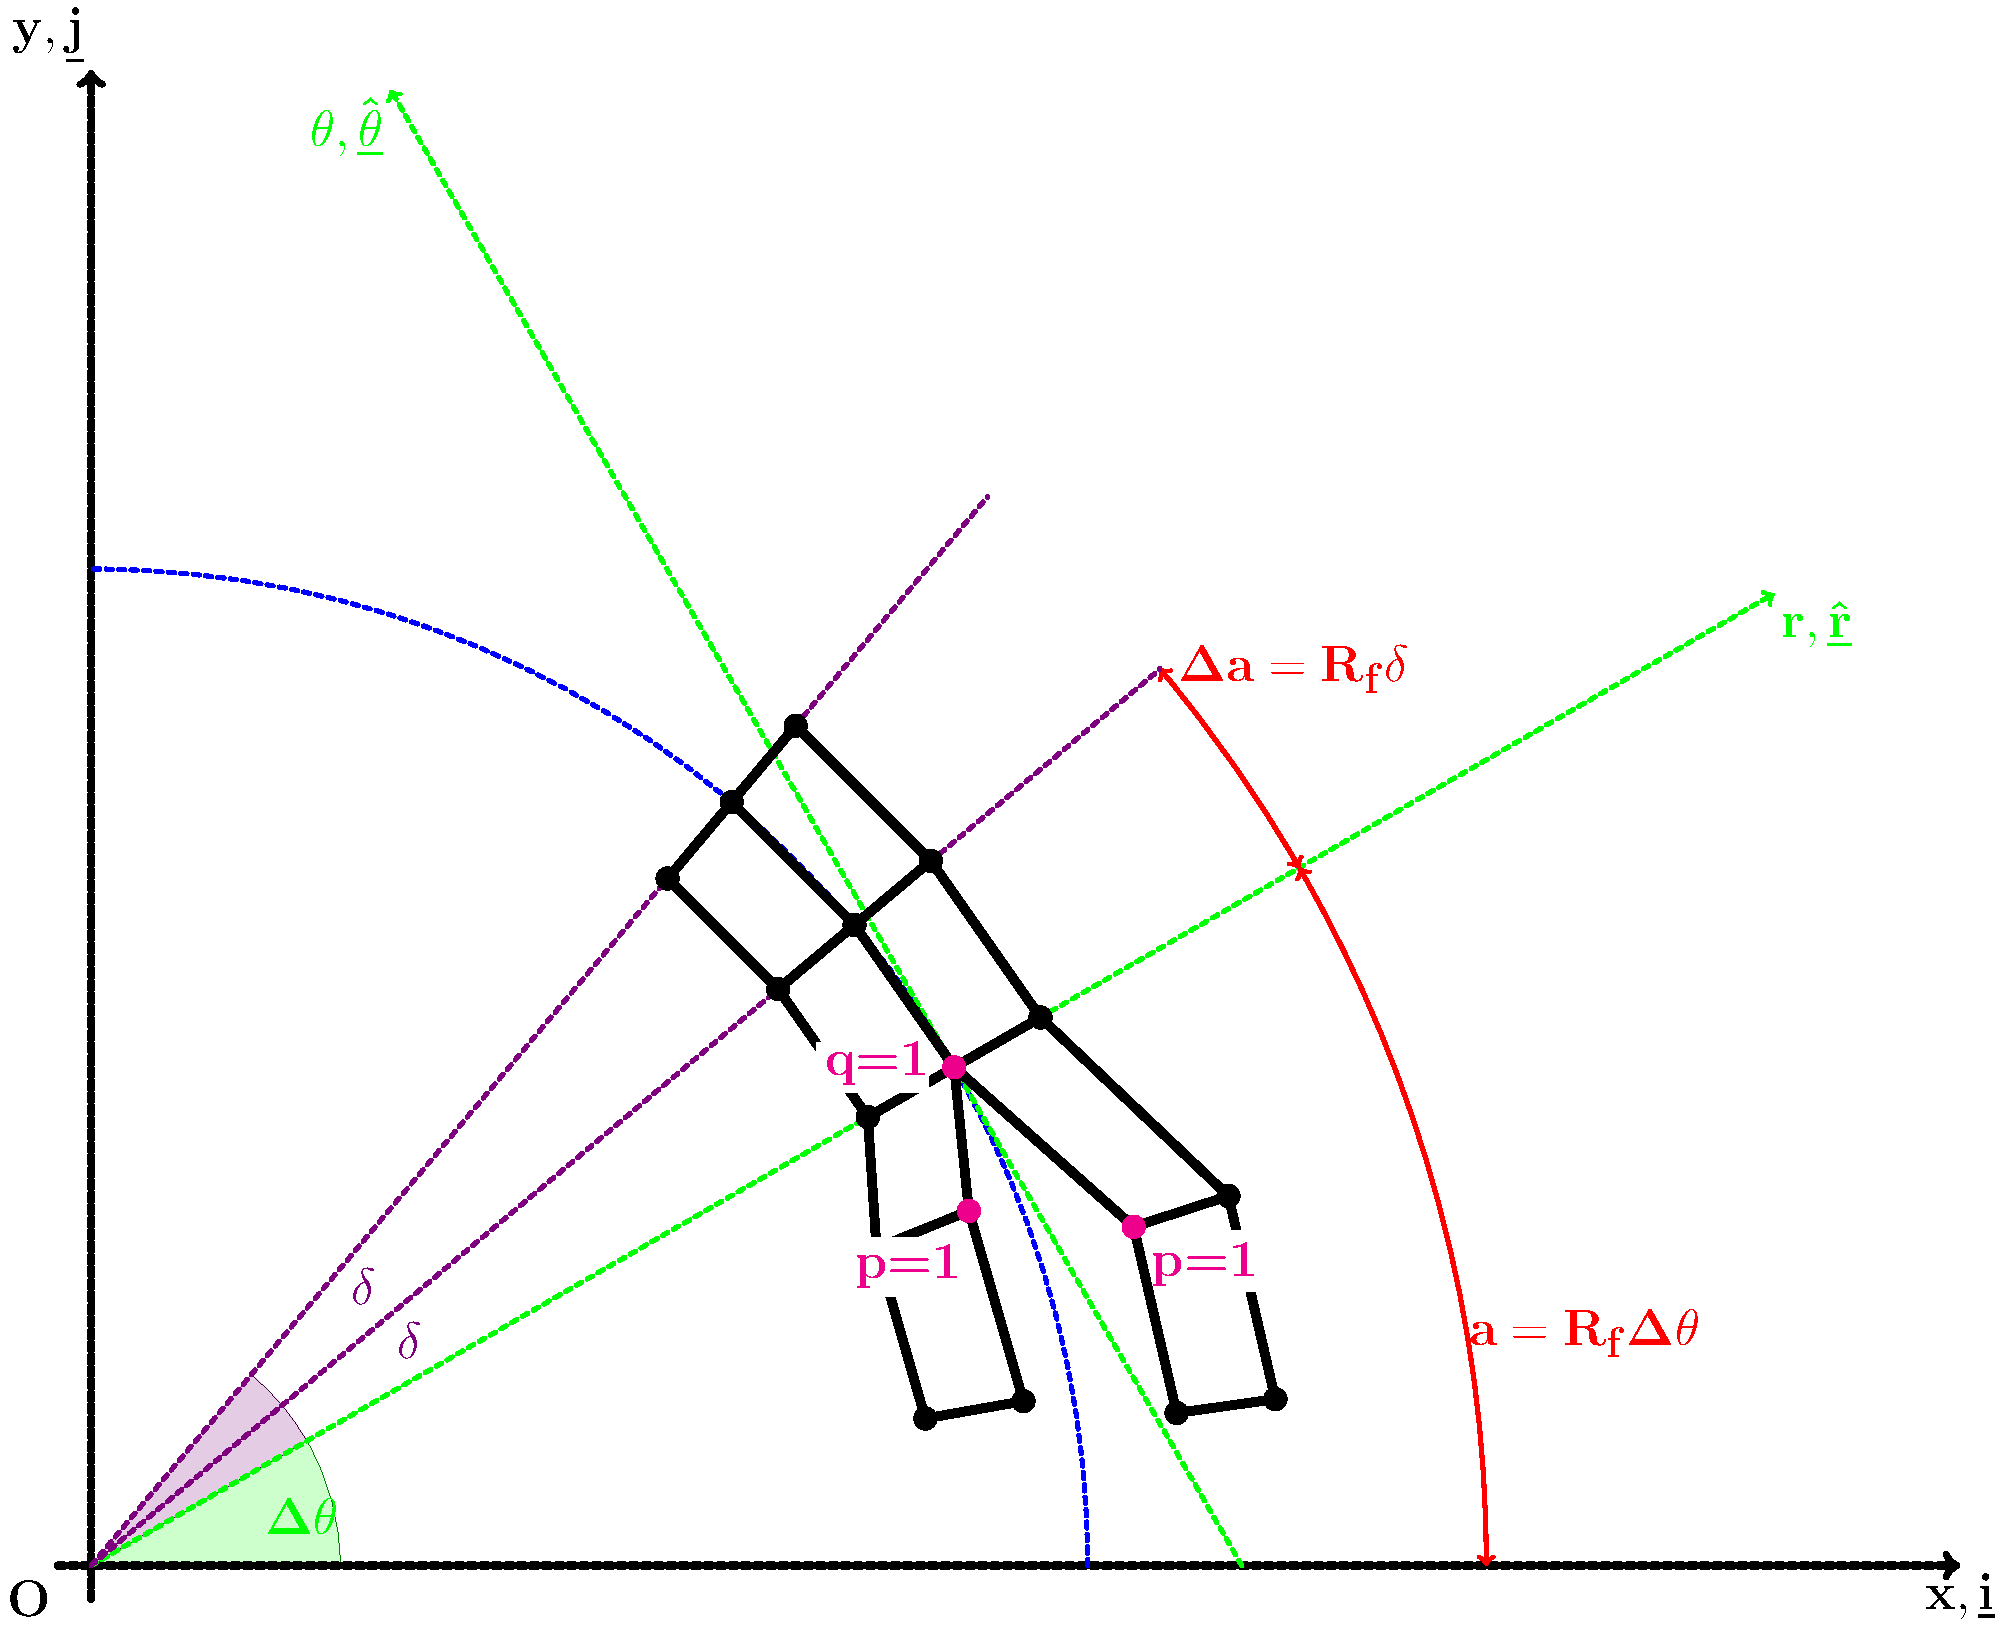
\includegraphics[width=\textwidth]{paperA/VCCT-linear.pdf}
       \caption{\added{Elements with $1^{st}$ order shape functions: $m=1$ and $p,q=1$.}}
    \end{subfigure}

    \begin{subfigure}[b]{0.8\textwidth}
        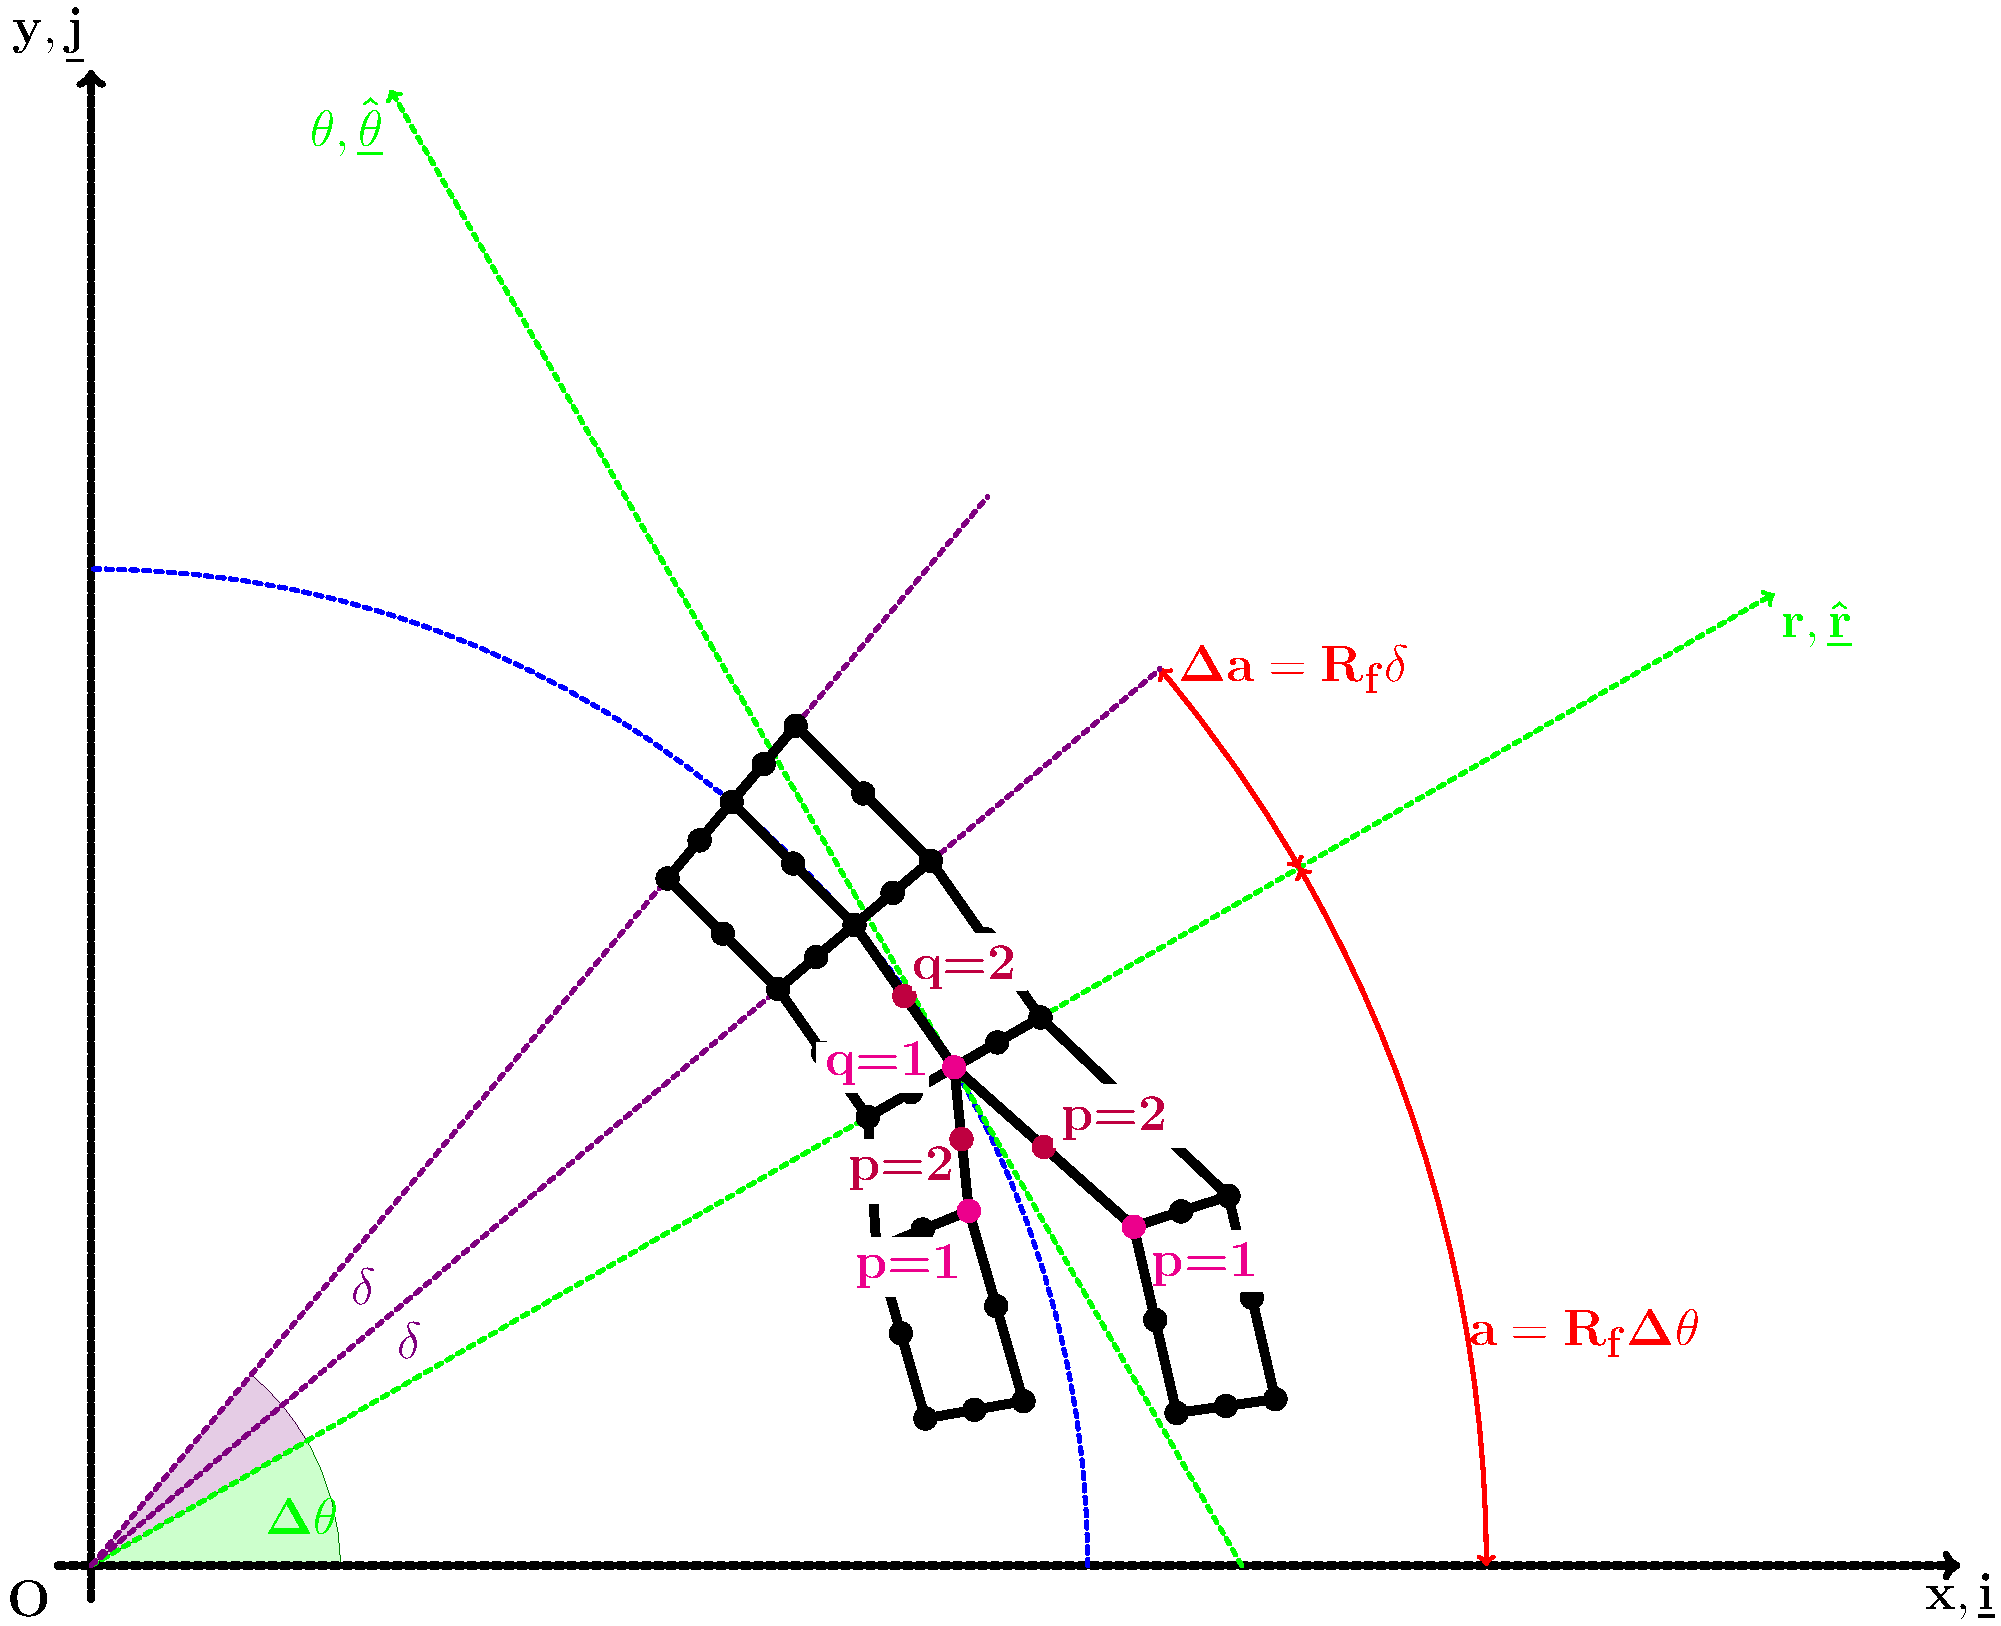
\includegraphics[width=\textwidth]{paperA/VCCT-quadratic.pdf}
       \caption{\added{Elements with $2^{nd}$ order shape functions: $m=2$ and $p,q=1,2$.}}
    \end{subfigure}

\caption{\added{Schematic of the mesh at the fiber/matrix interface crack tip.}}\label{chap3:paperA:fig:vcctmesh}
\end{figure}

%%%%%%%%%%%%%%%%%%%%%%%%%%%%%%%%%%%%%%%%%%%%%%%%%%%%%%%%%%%%%%%%%%%%%%%
%      Paper B
%%%%%%%%%%%%%%%%%%%%%%%%%%%%%%%%%%%%%%%%%%%%%%%%%%%%%%%%%%%%%%%%%%%%%%%
\section{Paper B}
\section*{Energy release rate of the fiber/matrix interface crack in UD composites under transverse loading: effect of the fiber volume fraction and of the distance to the free surface and to non-adjacent debonds}

%%%%%%%%%%%%%%%%%%%%%%%%%%%%%%%%%%%%%%%%%%%%%%%%%%%%%%%%%%%%%%%%%%%%%%%
%      Paper C
%%%%%%%%%%%%%%%%%%%%%%%%%%%%%%%%%%%%%%%%%%%%%%%%%%%%%%%%%%%%%%%%%%%%%%%
\section{Paper C}
\section*{Effect of the proximity to the $\mathbf{0^{\circ}/90^{\circ}}$ interface on Energy Release Rate of fiber/matrix interface crack growth in the  $\mathbf{90^{\circ}}$-ply of a cross-ply laminate under tensile loading}

%%%%%%%%%%%%%%%%%%%%%%%%%%%%%%%%%%%%%%%%%%%%%%%%%%%%%%%%%%%%%%%%%%%%%%%
%      Paper D
%%%%%%%%%%%%%%%%%%%%%%%%%%%%%%%%%%%%%%%%%%%%%%%%%%%%%%%%%%%%%%%%%%%%%%%
\section{Paper D}
\section*{Growth of interface cracks on consecutive fibers: on the same or on the opposite sides?}

%%%%%%%%%%%%%%%%%%%%%%%%%%%%%%%%%%%%%%%%%%%%%%%%%%%%%%%%%%%%%%%%%%%%%%%
%      Paper E
%%%%%%%%%%%%%%%%%%%%%%%%%%%%%%%%%%%%%%%%%%%%%%%%%%%%%%%%%%%%%%%%%%%%%%%
\section{Paper E}
\section*{Estimating the average size of fiber/matrix interface cracks in ud and cross-ply laminates}


\makebib
%\end{bibunit}

%%%%%%%%%%%%%%%%%%%%%%%%%%%%%%%%%%%%%%%%%%%%%%%%%%%%%%%%%%%%%%%%%%%%
%% Begin Part II - Collection of papers
%%%%%%%%%%%%%%%%%%%%%%%%%%%%%%%%%%%%%%%%%%%%%%%%%%%%%%%%%%%%%%%%%%%%

\makepartpage{Part II}%
\startpapers

%-------------------------------------------------------------------
\def\paperheader{Paper A}
\def\papertitle{Finite Element solution of the fiber/matrix interface crack problem: convergence properties and mode mixity of the Virtual Crack Closure Technique}
\def\paperauthorstring{Luca Di Stasio and Zoubir Ayadi}
\def\referencestring{Finite Elements in Analysis and Design, 2019.}
\def\copyrightstring{2019, The Authors.}

% The definitions above could just as well be put directly into the function
% call below, but were explicitly defined to more clearly illustrate the
% use of the function \makepaper.

\newrefsection
\makepapersubmitted
  {\paperheader}
  {\papertitle}
  {\paperauthorstring}
  {\referencestring}
  {\copyrightstring}

% The actual contents is imported by un-commenting the \input line below.
% Make sure the file exist.

\thispagestyle{plain}
\begin{center}
\Large\textbf{Finite Element solution of the fiber/matrix interface crack problem: convergence properties and mode mixity of the Virtual Crack Closure Technique}\\
\vspace{10mm}
\normalsize Luca Di Stasio$^{1,2}$ and Zoubir Ayadi$^{2}$\\
\vspace{5mm}
\normalsize $^{1}$Lule\aa\ University of Technology, University Campus, SE-97187 Lule\aa, Sweden\\
\normalsize $^{2}$Universit\'e de Lorraine, EEIGM, IJL, 6 Rue Bastien Lepage, F-54010 Nancy, France\\
\vspace{15mm}
\textbf{Abstract}\\
\end{center}

The bi-material interface arc crack has been the focus of interest in the composite community, where it is usually referred to as the fiber-matrix interface crack. In this work, we investigate the convergence properties of the Virtual Crack Closure Technique (VCCT) when applied to the evaluation of the Mode I, Mode II and total Energy Release Rate of the fiber-matrix interface crack in the context of the Finite Element Method (FEM). We first propose a synthetic vectorial formulation of the VCCT. Thanks to this formulation, we study the convergence properties of the method, both analytically and numerically. It is found that Mode I and Mode II Energy Release Rate (ERR) possess a logarithmic dependency with respect to the size of the elements in the crack tip neighborhood, while the total ERR is independent of element size.

\vspace{5mm}

\textbf{Keywords:} Fiber/matrix interface crack, Bi-material interface arc crack, Linear Elastic Fracture Mechanics (LEFM), Virtual Crack Closure Technique (VCCT), Mode separation, Convergence

\section{Introduction}\label{paperA:sec:intro}

Bi-material interfaces represent the basic load transfer mechanism at the heart of Fiber Reinforced Polymer Composite (FRPC) materials. They are present at the macroscale, in the form of adhesive joints; at the mesoscale, as interfaces between layers with different orientations; at the microscale, as fiber-matrix interfaces. Bi-material interfaces have for long attracted the attention of researchers in Fracture Mechanics~\cite{Comninou1990,Hills1993}, due to their hidden complexity.\\
The problem was first addressed in the 1950's by Williams~\cite{Williams1959}, who derived through a linear elastic asymptotic analysis the stress distribution around an \emph{open} crack (i.e. with crack faces nowhere in contact for any size of the crack) between two infinite half-planes of dissimilar materials. He found the existence of a strong oscillatory behavior in the stress singularity at the crack tip of the form

\begin{equation}\label{paperA:eq:singularitywilliams}
r^{-\frac{1}{2}}\sin\left(\varepsilon\log r\right)\quad\text{with}\quad\varepsilon=\frac{1}{2\pi}\log\left(\frac{1-\beta}{1+\beta}\right),
\end{equation}

in both Mode I and Mode II. In Eq.~\ref{paperA:eq:singularitywilliams}, $\beta$ is one of the two parameters introduced by Dundurs~\cite{Dundurs1969} to characterize bi-material interfaces:

\begin{equation}\label{paperA:eq:dundursbeta}
\beta=\frac{\mu_{2}\left(\kappa_{1}-1\right)-\mu_{1}\left(\kappa_{2}-1\right)}{\mu_{2}\left(\kappa_{1}+1\right)+\mu_{1}\left(\kappa_{2}+1\right)}
\end{equation}

where $\kappa=3-4\nu$ in plane strain and $\kappa=\frac{3-4\nu}{1+\nu}$ in plane stress, $\mu$ is the shear modulus, $\nu$ Poisson's coefficient, and indexes $1,2$ refer to the two bulk materials joined at the interface. Defining $a$ as the length of the crack, it was found that the size of the oscillatory region is in the order of $10^{-6}a$~\cite{Erdogan1963}. Given the oscillatory behaviour of the crack tip singularity of Eq.~\ref{paperA:eq:singularitywilliams}, the definition of Stress Intensity Factor (SIF) $\lim_{r\rightarrow 0}\sqrt{2\pi r}\sigma$ diverges and ceases to be valid~\cite{Comninou1990}. It implies that the Mode mixity problem at the crack tip is ill-posed.\\
It was furthermore observed, always in the context of Linear Elastic Fracture Mechanics (LEFM), that an interpenetration zone exists close to the crack tip~\cite{England1965,Malyshev1965} with a length in the order of $10^{-4}a$~\cite{England1965}. Following conclusions firstly proposed in~\cite{Malyshev1965}, the presence of a \emph{contact zone} in the crack tip neighborhood, of a length to be determined from the solution of the elastic problem, was introduced in~\cite{Comninou1977} and shown to provide a physically consistent solution to the straight bi-material interface crack problem.\\
The curved bi-material interface crack, more often refered to as the fiber-matrix interface crack (or debond) due to its relevance in FRPCs, was first treated by England~\cite{England1966} and by Perlman and Sih~\cite{Perlman1967}, who provided the analytical solution of stress and displacement fields for a circular inclusion with respectively a single debond and an arbitrary number of debonds. Building on their work, Toya~\cite{Toya1974} particularized the solution and provided the expression of the Energy Release Rate (ERR) at the crack  tip. The same problems exposed previously for the \emph{open} straight bi-material crack were shown to exist also for the \emph{open} fiber-matrix interface crack: the presence of strong oscillations in the crack tip singularity and onset of crack face interpenetration at a critical flaw size.\footnote{For the fiber-matrix interface crack, flaw size is measured in terms of the angle $\Delta\theta$ subtended by half of the arc-crack, i.e. \replaced{$a=2\Delta\theta R_{f}$ where $R_{f}$ is the inclusion (fiber) radius and $\Delta\theta$ is expressed in radians }{$a=2\Delta\theta$}.}\\
In order to treat cases more complex than the single partially debonded fiber in an infinite matrix of~\cite{England1966,Perlman1967,Toya1974}, numerical studies followed. In the 1990's, Par{\'{\i}}s and collaborators~\cite{Paris1996} developed a Boundary Element Method (BEM) with the use of discontinuous singular elements at the crack tip and the Virtual Crack Closure Integral (VCCI)~\cite{Irwin1958} for the evaluation of the Energy Release Rate (ERR). They validated their results~\cite{Paris1996} with respect to Toya's analytical solution~\cite{Toya1974} and analyzed the effect of BEM interface discretization on the stress field in the neighborhood of the crack tip~\cite{DelCano1997}. Following Comninou's work on the straight crack~\cite{Comninou1977}, they furthermore recognized the importance of contact to retrieve a physical solution avoiding interpenetration~\cite{Paris1996} and studied the effect of the contact zone on debond ERR~\cite{Varna1997a}. Their algorithm was then applied to investigate the fiber-matrix interface crack under different geometrical configurations and mechanical loadings ~\cite{Paris2007,Correa2007,Correa2011,Correa2013,Correa2014,Sandino2016,Sandino2018}.\\
Recently the Finite Element Method (FEM) was also applied to the solution of the fiber-matrix interface crack problem~\cite{Zhuang2018,Varna2017,Zhuang2018a}, in conjunction with the Virtual Crack Closure Technique (VCCT)~\cite{Rybicki1977,Krueger2004} for the evaluation of the ERR at the crack tip. In~\cite{Zhuang2018}, the authors validated their model with respect to the BEM results of~\cite{Paris1996}, but no analysis of the effect of the discretization in the crack tip neighborhood comparable to~\cite{DelCano1997} was proposed. \replaced{Thanks to the interest in evaluating the ERR of interlaminar delamination, different studies exist in the literature on the effect of mesh discretization on Mode I and Mode II ERR of the straight bi-material interface crack when evaluated with the VCCT in the context of the FEM (see for example~\cite{Krueger2013} for a review). An early result on the problem is available in~\cite{Sun1987}. Here the authors evaluated with the Virtual Crack Closure Technique Mode I and Mode II Energy Release Rate of both a central crack and an edge crack at the interface between two 2D plates of different isotropic materials subjected to tensile loading. They showed analytically that the total ERR $G$ is well defined while Mode I and Mode II ERR, respectively $G_{I}$ and $G_{II}$, do not converge. They confirmed their analytical derivations numerically by solving the two problems with the Finite Element Method and evaluating the ERR with the VCCT. Referring to the crack length as $a$ and to the length of an element at the crack tip as $\Delta a$, they found that the total ERR was independent of normalized element size $\nicefrac{\Delta a}{a}$ while $G_{I}$ and $G_{II}$ were dependent on assumed crack extension, i.e. element size at the crack tip. In particular, they showed a decreasing $G_{I}$ and an increasing $G_{II}$ with decreasing element size for both crack configurations. The same analysis was conducted, and analogous results obtained, in~\cite{Sun1989} for a central crack under either far-field tensile or shear loading between two orthotropic materials in 2D and in~\cite{Manoharan1990} for a central crack subjected to far-field tension between two orthotropic solids in 3D. The convergence of VCCT-based mode decomposition was analyzed in~\cite{Raju1988} for edge delaminations in laminated composites subjected to tensile loading coplanar and normal to crack propagation direction in a quasi-3D setting. Again, it was observed that the total ERR was independent of mesh size while Mode I and Mode II ERR showed dependency and no convergence could be established. In this configuration however, it was found that $G_{I}$ increases and $G_{II}$ decreases with decreasing element size. The application of the VCCT to the problem of composite skin-stiffener debonding was considered in~\cite{Glaessgen1998} in conjunction with 2D plate elements, where the authors studied the effect of different combinations of adherends' layup, thickness and fiber orientation at the interface on Mode decomposition. Only in the case of skin and stiffener with the same layup, same thickness and identical fiber orientation at the interface, Mode I and Mode II were found to be independent of mesh size. In all other cases, $G_{I}$ and $G_{II}$ were dependent on assumed crack extension and showed a trend similar to the one in~\cite{Raju1988}. The absence of a converging Mode-decomposed solution with the VCCT has motivated proposals for alternative solution. In~\cite{Agrawal2006}, the authors analyze several proposals of mode-mixity parameters and suggest a correction to the VCCT-based mode-mixity ratio by assuming a reference characteristic length. The authors themselves however admit that this characteristic length has no physical interpretation. In~\cite{Wang2013}, the problem of Mode-decomposition is solved through the development of analytical relations based on Euler and Timoshenko beam models. It is however well suited only for those configurations that can be split into beam elements, such as the Double Cantilever Beam (DCB) specimen. }{Thanks to the interest in evaluating the ERR of interlaminar delamination, different studies exist in the literature on the effect of mesh discretization on Mode I and Mode II ERR of the bi-material interface crack when evaluated with the VCCT in the context of the FEM.} \\\deleted{However,} No comparable analysis can be found in the literature on Mode separation and convergence analysis of the VCCT when applied to the fiber-matrix interface crack (circular bi-material interface crack) problem in the context of a linear elastic FEM solution. In the present article, we first present the FEM formulation of the problem, together with the main geometrical characteristics, material properties, boundary conditions and loading. We then propose a vectorial formulation of the VCCT and express Mode I and Mode II ERR in terms of FEM natural variables. \replaced{Differently from the usual approach found in the literature, we do not express $G_{I}$ and $G_{II}$ as functions of stress and displacement fields using the results from complex analysis. We instead focus on the mathematical structure of the 1-step VCCT in the context of the Finite Element Method and write the crack tip forces as a linear combination of the crack faces displacements at the crack tip (plus a term representing the influence of the rest of the model). The ERR is consequently a quadratic function of the crack faces displacements. Given that, if the FEM solution is converging, stress and displacement fields are characterized by the oscillating singularity of Equation~\ref{paperA:eq:singularitywilliams}, it is possible to evaluate the behavior of the VCCT-calculated Energy Release Rate in the limit of crack tip element size going to zero. We are thus able to derive analytically a functional form of the dependency of the ERR on crack tip element size. Finally, the functional form thus derived is compared to the numerical results obtained with the Finite Element Method.}{With this tool, we derive an analytical estimate of the ERR convergence and compare it with numerical results.}

\section{FEM formulation of the fiber-matrix interface crack problem}\label{paperA:sec:femmodel}

In order to investigate the fiber-matrix interface crack problem, a 2-dimensional model of a single fiber inserted in a rectangular matrix element is considered (see Figure~\ref{paperA:fig:modelschem}). Total element length and height are respectively $2L$ and $L$, where $L$ is determined by the fiber radius $R_{f}$ and the fiber volume fraction $V_{f}$ by

\begin{equation}\label{paperA:eq:LVf}
L=\frac{R_{f}}{2}\sqrt{\frac{\pi}{V_{f}}}.
\end{equation}

The fiber radius $R_{f}$ is assumed to be equal to $1\ \mu m$. This choice is not dictated by physical considerations but for simplicity. It is thus useful to remark that, in a linear elastic solution as the one considered in the present work, the ERR is proportional to the geometrical dimensions of the model and, consequently, recalculation of the ERR for fibers of any size requires a simple multiplication.

\begin{figure}[!h]
\centering
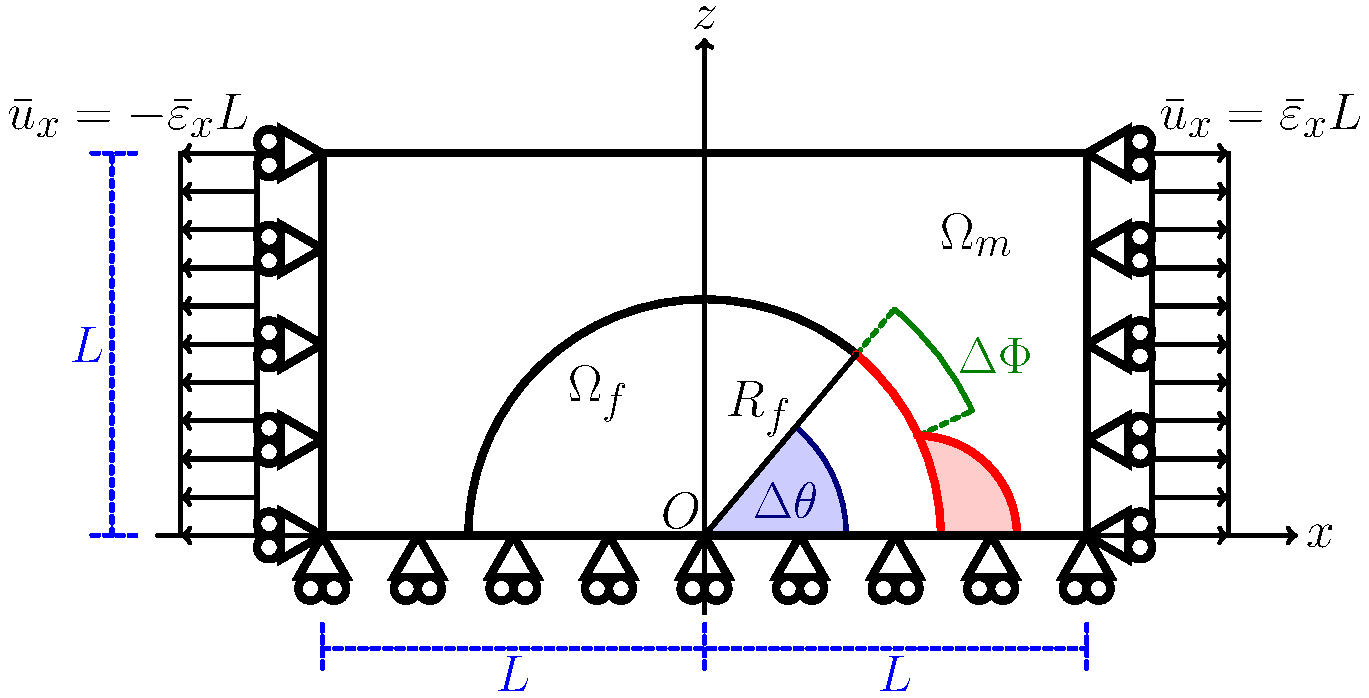
\includegraphics[width=\textwidth]{paperA/RUC.pdf}
\caption{Schematic of the model with its main parameters.}\label{paperA:fig:modelschem}
\end{figure}

As shown in Fig.~\ref{paperA:fig:modelschem}, the debond is placed symmetrically with respect to the $x$ axis and its size is characterized by the angle $\Delta\theta$ (which makes the full debond size equal to $2\Delta\theta$ and the full crack length equal to $R_{f}2{\Delta\theta}$). A region $\Delta\Phi$ of unknown size appears at the crack tip for large debond sizes (at least $\geq 60^{\circ}-80^{\circ}$), in which the crack faces are in contact with each other and free to slide. Frictionless contact is thus considered between the two crack faces to allow free sliding and avoid interpenetration. Symmetry with respect to the $x$ axis is applied on the lower boundary while the upper surface is left free. Kinematic coupling on the $x$-displacement is applied along the left and right sides of the model in the form of a constant $x$-displacement $\pm\bar{\varepsilon}_{x} L$, which corresponds to transverse strain $\bar{\varepsilon}_{x}$ equal to $1\%$ in the results here presented.

\begin{table}[!htbp]
 \centering
 \caption{Summary of the mechanical properties of fiber and matrix. $E$ stands for Young's modulus, $\mu$ for shear modulus and $\nu$ for Poisson's ratio.}
 \begin{tabular}{cccc}
\textbf{Material} & \textbf{$E\left[GPa\right]$}\ & \textbf{$\mu\left[GPa\right]$} & \textbf{$\nu\left[-\right]$} \\
\midrule
Glass fiber    & 70.0  & 29.2   & 0.2  \\
Epoxy    & 3.5    & 1.25   & 0.4
\end{tabular}
\label{paperA:tab:phaseprop}
\end{table}

The model problem is solved with the Finite Element Method (FEM) within the Abaqus environment, a commercial FEM software~\cite{abq12}. The model is meshed with second order, 2D, plane strain triangular (CPE6) and rectangular (CPE8) elements. A regular mesh of rectangular elements with almost unitary aspect ratio is used at the crack tip. The angular size $\delta$ of an element in the crack tip neighborhood represents the main parameter of the numerical analysis. The crack faces are modeled as element-based surfaces and a small-sliding contact pair interaction with no friction is imposed between them. The Mode I, Mode II and total Energy Release Rates (ERRs) (respectively referred to as $G_{I}$, $G_{II}$ and $G_{TOT}$) are evaluated using the VCCT~\cite{Krueger2004}, implemented in a in-house Python routine. A glass fiber-epoxy system is considered in the present work, and it is assumed that their response lies always in the linear elastic domain. The elastic properties of glass fiber and epoxy are reported in Table~\ref{paperA:tab:phaseprop}.

\section{Vectorial formulation of the Virtual Crack Closure Technique (VCCT)}

In order to express the VCCT formulation of the ERR in terms of FEM variables, we need to introduce a few rotation matrices in order to represent the discretized representation (FE mesh) of a crack along a circular interface. The position of the crack tip is characterized by the angular size of the crack (see Sec.~\ref{paperA:sec:femmodel} and Fig.~\ref{paperA:fig:modelschem} for reference) and the rotation corresponding to the crack tip reference frame is represented by the matrix $\underline{\underline{R}}_{\Delta\theta}$ defined as

\begin{equation}\label{paperA:eq:Rmatrix}
\underline{\underline{R}}_{\Delta\theta}=\begin{bmatrix}
\cos\left(\Delta\theta\right) & \sin\left(\Delta\theta\right) \\
-\sin\left(\Delta\theta\right) & \cos\left(\Delta\theta\right)
\end{bmatrix}.
\end{equation}

Nodes belonging to the elements sharing the crack tip are involved in the VCCT estimation of the ERR and it is assumed that, given a sufficiently fine discretization, they are aligned with the crack propagation direction defined at the crack tip.

\begin{figure}[!h]
\centering
    \begin{subfigure}[b]{0.8\textwidth}
        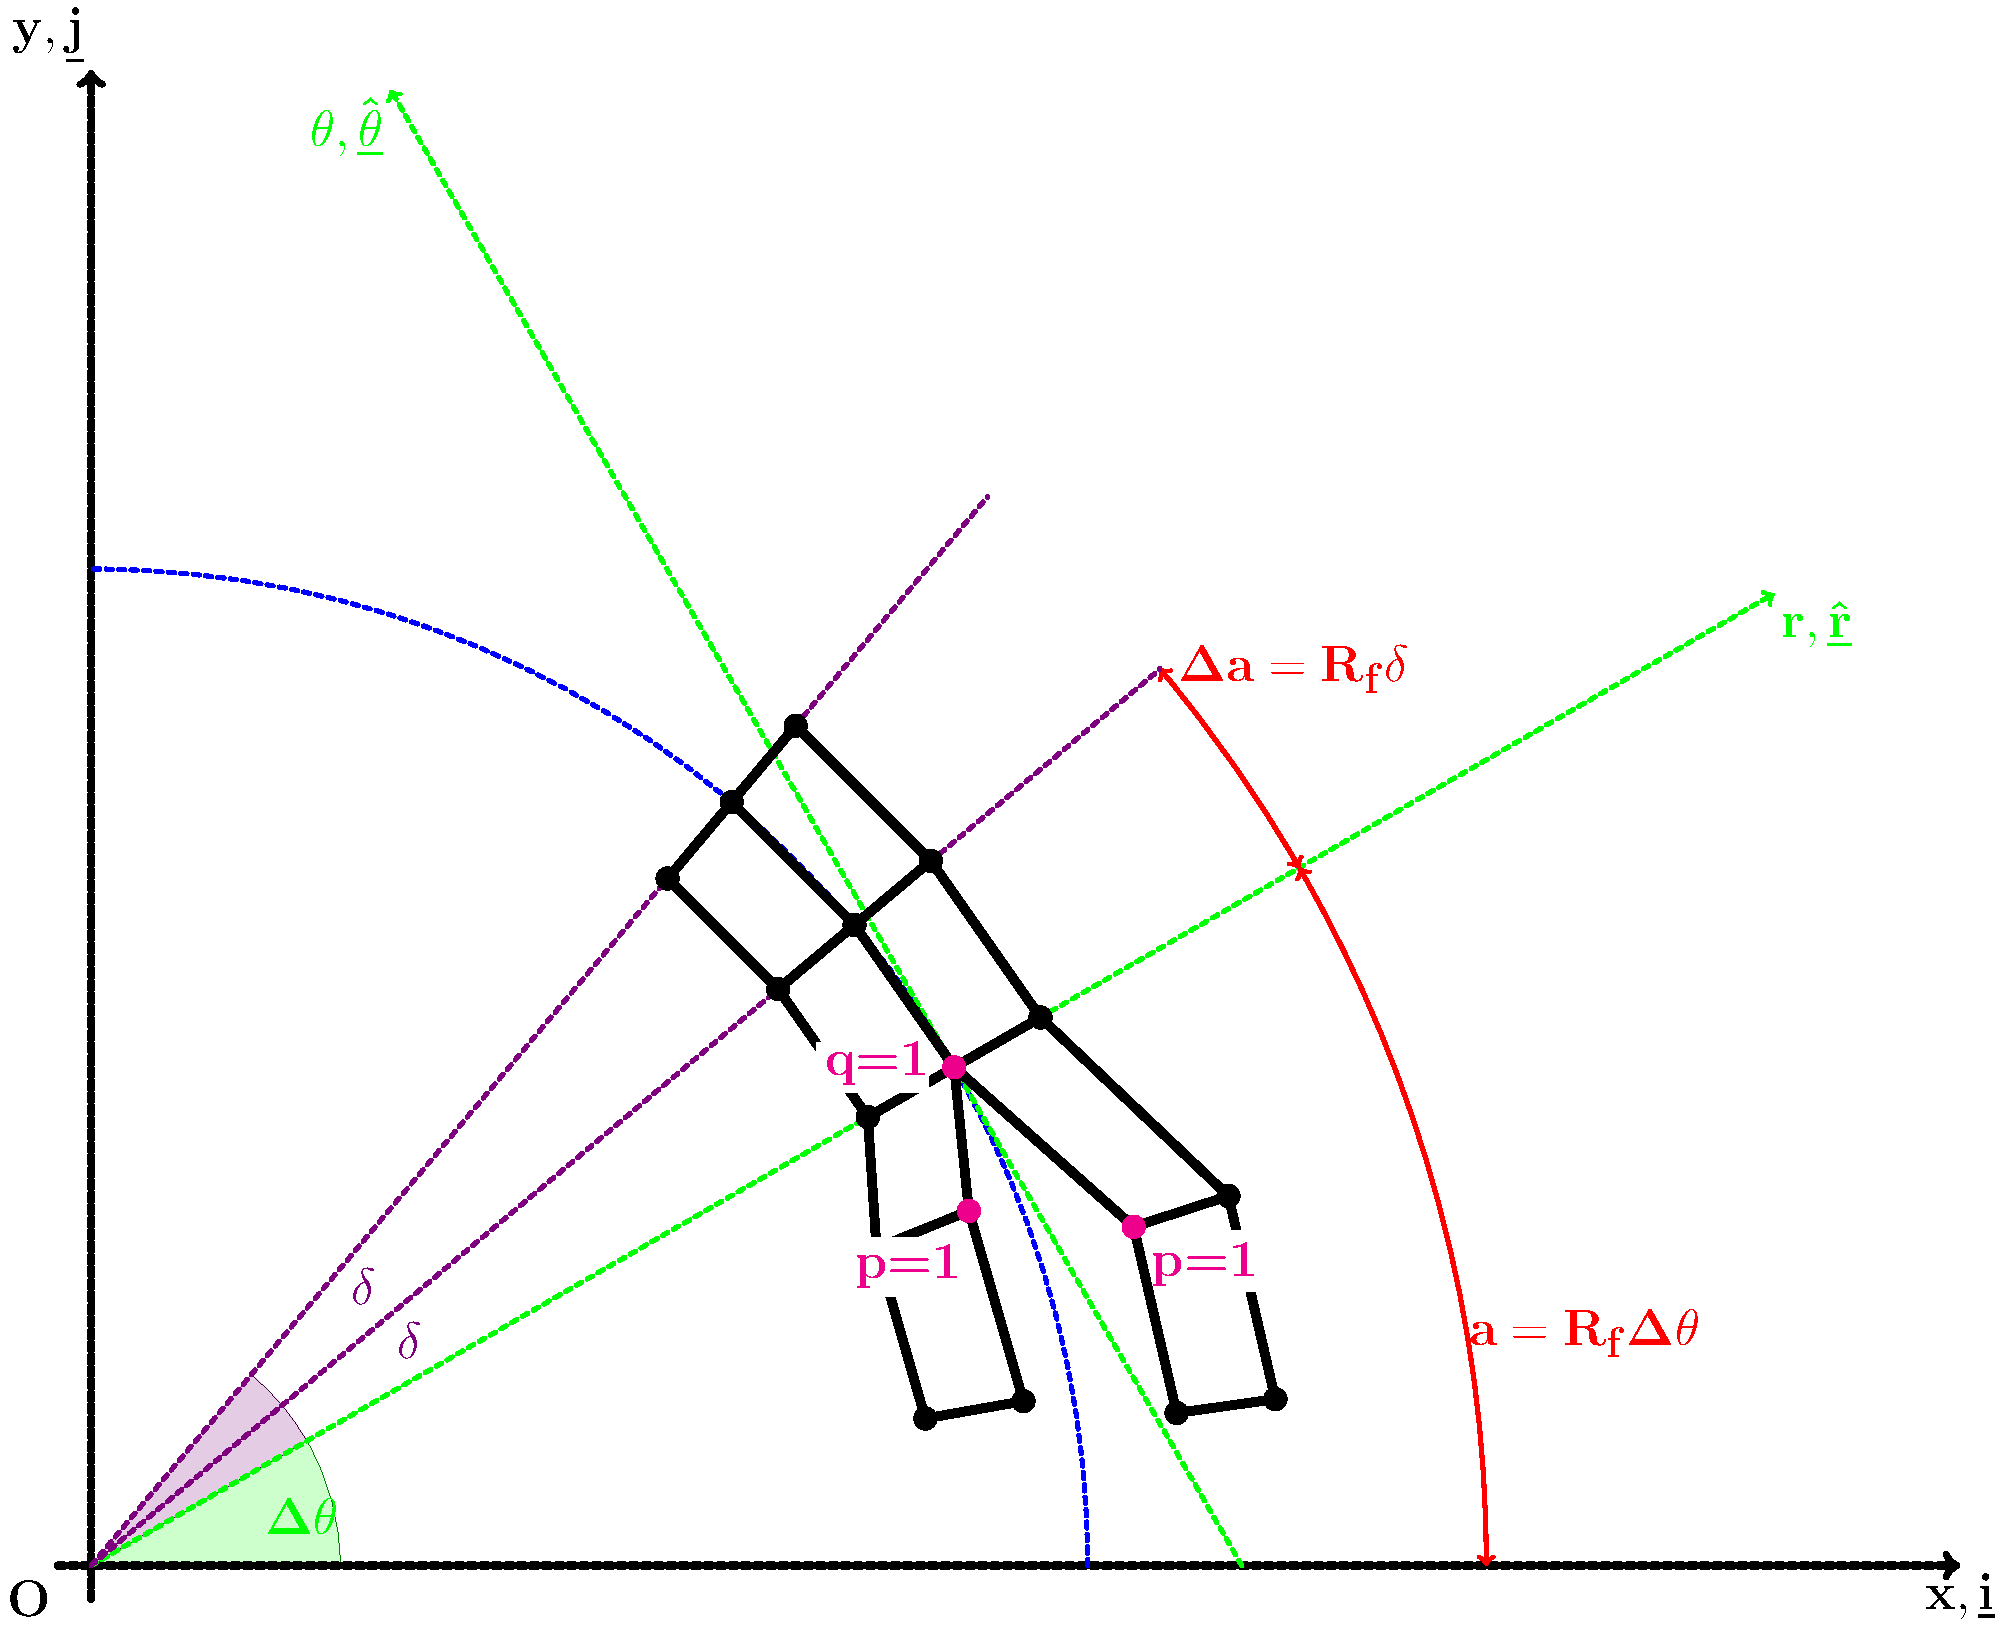
\includegraphics[width=\textwidth]{paperA/VCCT-linear.pdf}
       \caption{\added{Elements with $1^{st}$ order shape functions: $m=1$ and $p,q=1$.}}
    \end{subfigure}

    \begin{subfigure}[b]{0.8\textwidth}
        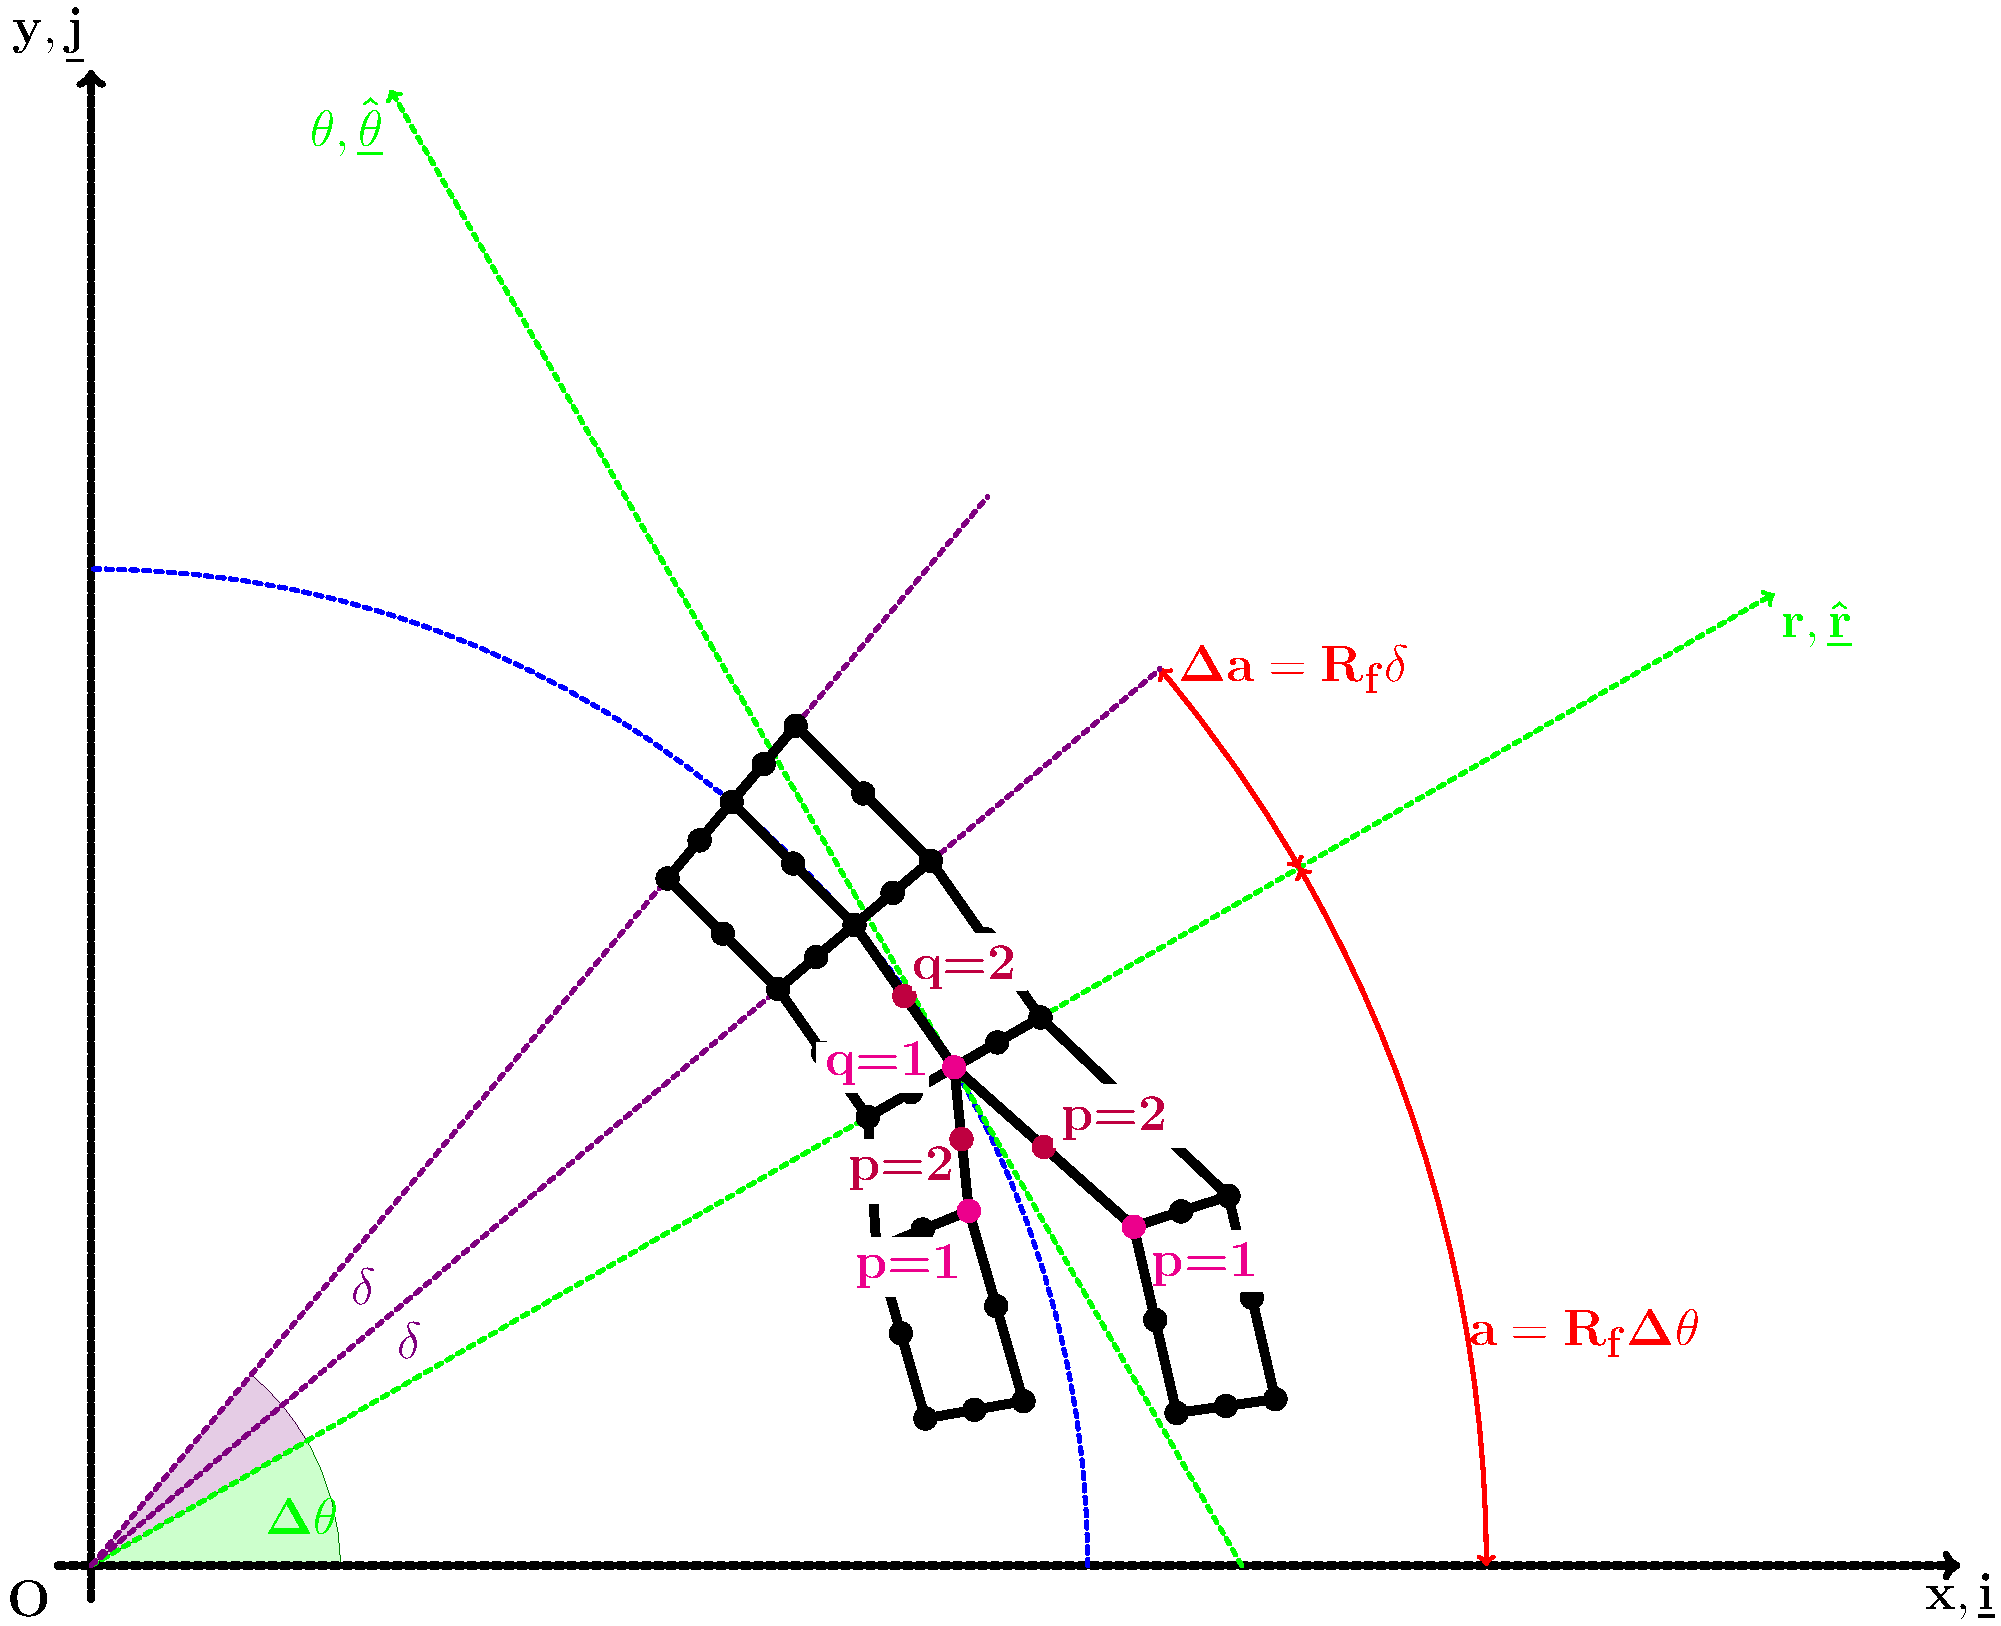
\includegraphics[width=\textwidth]{paperA/VCCT-quadratic.pdf}
       \caption{\added{Elements with $2^{nd}$ order shape functions: $m=2$ and $p,q=1,2$.}}
    \end{subfigure}

\caption{\added{Schematic of the mesh at the fiber/matrix interface crack tip.}}\label{paperA:fig:vcctmesh}
\end{figure}

However, irrespectively of how small the elements in the crack tip neighborhood are, a misalignment always exists with respect to the assumed crack propagation direction (in the crack tip reference frame). This is measured by the matrices $\underline{\underline{P}}_{\delta}\left(p\right)$, defined as

\begin{equation}\label{paperA:eq:Pmatrix}
\underline{\underline{P}}_{\delta}\left(p\right)=\begin{bmatrix}
\cos\left(\left(1+\frac{1-p}{m}\right)\delta\right) & \sin\left(\left(1+\frac{1-p}{m}\right)\delta\right) \\
-\sin\left(\left(1+\frac{1-p}{m}\right)\delta\right) & \cos\left(\left(1+\frac{1-p}{m}\right)\delta\right)
\end{bmatrix}
\end{equation}

 and $\underline{\underline{Q}}_{\delta}\left(q\right)$, equal to

\begin{equation}\label{paperA:eq:Qmatrix}
\underline{\underline{Q}}_{\delta}\left(q\right)=\begin{bmatrix}
\cos\left(\frac{q-1}{m}\delta\right) & \sin\left(\frac{q-1}{m}\delta\right) \\
-\sin\left(\frac{q-1}{m}\delta\right) & \cos\left(\frac{q-1}{m}\delta\right)
\end{bmatrix},
\end{equation}

respectively for the free and bonded nodes involved in the VCCT estimation. In Eqs.~\ref{paperA:eq:Pmatrix} and~\ref{paperA:eq:Qmatrix}, $\delta$ is the angular size of an element in the crack tip neighborhood (see Sec.~\ref{paperA:sec:femmodel} and Fig.~\ref{paperA:fig:modelschem}), $m$ is the order of the element shape functions and \replaced{$p,q=1,\dots,m$}{ $p,q$} are indices referring to the nodes belonging respectively to free and bonded elements sharing the crack tip. \added{Figure~\ref{paperA:fig:vcctmesh} shows the $p,q$-based numbering of nodes at the crack tip in the case of elements with linear and quadratic (serendipity) shape functions.} Introducing the permutation matrix


\begin{equation}
\underline{\underline{P}}_{\pi}=\begin{bmatrix}
0 & 1\\
-1& 0
\end{bmatrix},
\end{equation}

it is possible to express the derivatives of rotation matrices $\underline{\underline{R}}_{\Delta\theta}$, $\underline{\underline{P}}_{\delta}$ and $\underline{\underline{Q}}_{\delta}$ with respect to their argument:

\begin{equation}\label{paperA:eq:rotmatdev}
\added{\frac{\partial \underline{\underline{R}}_{\Delta\theta}}{\partial \Delta\theta}=\underline{\underline{P}}_{\pi}\cdot\underline{\underline{R}}_{\Delta\theta},\quad\frac{\partial \underline{\underline{P}}_{\delta}}{\partial \delta}=\left(1+\frac{1-p}{m}\right)\underline{\underline{P}}_{\pi}\cdot\underline{\underline{P}}_{\delta},\quad\frac{\partial \underline{\underline{Q}}_{\delta}}{\partial \delta}=\frac{q-1}{m}\underline{\underline{P}}_{\pi}\cdot\underline{\underline{Q}}_{\delta}}.
\end{equation}

By means of Eqs.~\ref{paperA:eq:Pmatrix} and~\ref{paperA:eq:Qmatrix}, we can express the crack tip forces $
\underline{F}_{xy}=\begin{bmatrix}
F_{x} \\
F_{y}
\end{bmatrix}$ and crack displacements  $
\underline{u}_{xy}=\begin{bmatrix}
u_{x} \\
u_{y}
\end{bmatrix}$ in the crack tip reference frame (where the tangential direction $\theta$ correspond to the direction of crack propagation) while taking into account the misalignment to the finite  discretization as

\begin{equation}\label{paperA:eq:FUrot}
\underline{F}_{r\theta}=\underline{\underline{Q}}_{\delta}\underline{\underline{R}}_{\Delta\theta}\underline{F}_{xy}\qquad\underline{u}_{r\theta}=\underline{\underline{P}}_{\delta}\underline{\underline{R}}_{\Delta\theta}\underline{u}_{xy}
\end{equation}

where $\underline{F}_{r\theta}=\begin{bmatrix}
F_{r} \\
F_{\theta}
\end{bmatrix}$ and $\underline{u}_{r\theta}=\begin{bmatrix}
u_{r} \\
u_{\theta}
\end{bmatrix}$.

The crack tip forces can be expressed as a function of the crack opening displacement as

\begin{equation}\label{paperA:eq:ctforce1}
\underline{F}_{xy}=\underline{\underline{K}}_{xy}\underline{u}_{xy}+\underline{\widetilde{F}}_{xy},
\end{equation}

where $\underline{\underline{K}}_{xy}$ is in general a full matrix of the form $\underline{\underline{K}}_{xy}=\begin{bmatrix}
K_{xx}  K_{xy}\\
K_{yx}  K_{yy}
\end{bmatrix}$ and $\underline{\widetilde{F}}_{xy}$ represents the effect of the rest of the FE solution through the remaining nodes of the elements attached to the crack tip. As such, the term $\underline{\widetilde{F}}_{xy}$ can be expressed as a linear combination of the solution vector $\underline{u}_{N}$ of nodal displacements of the form $\underline{\underline{\widetilde{K}}}_{N}\underline{u}_{N}$. Equation~\ref{paperA:eq:ctforce1} thus become

\begin{equation}\label{paperA:eq:ctforce2}
\underline{F}_{xy}=\underline{\underline{K}}_{xy}\underline{u}_{xy}+\underline{\underline{\widetilde{K}}}_{N}\underline{u}_{N}.
\end{equation}

An exemplifying derivation of the relationships expressed in Equations~\ref{paperA:eq:ctforce1} and~\ref{paperA:eq:ctforce2} can be found in \ref{paperA:app:ctforcesexample}. \replaced{It is worthwhile to observe that another author~\cite{Valvo2011,Valvo2015} proposes a similar relationship, but in terms of flexibility $\underline{u}=\underline{\underline{C}}\underline{F}$. In~\cite{Valvo2011,Valvo2015}, Valvo expresses the forces at the crack tip as a (linear) function of the crack faces displacements at the same point. The technique analyzed in~\cite{Valvo2011,Valvo2015} is the 2-steps VCCT~\cite{Krueger2004}: given a structure with a crack of length $a$, a first simulation is run to compute the forces at the crack tip and, in the case, at the internal nodes of the first bonded element for $p$-refined meshes; then, a second simulation is conducted with the crack extended by $\Delta a$, where in practice $\Delta a$ is the length of the element at the crack tip, and crack faces displacements are evaluated at the same nodes, now released, where previously forces were extracted. The Energy Release Rate is computed as the product of forces and displacements evaluated at the same nodes. The 2-steps VCCT adheres more strictly to the principle of the crack closute integral~\cite{Irwin1958,Irwin1957}: the work needed to open the crack by $\delta a$ (Energy Release Rate) is equal in magnitude to the work required to close it by the same amount. Forces and displacements should be thus evaluated at the same point respectively in the closed and open crack configuration. In this paper, we consider on the other hand the 1-step VCCT~\cite{Krueger2004}: if the size of the elements at the crack tip is sufficiently small, the error committed by approximating the crack faces displacements at the crack tip with those one element before is negligible. This in turn eliminates the need for a second simulation and thus cut the required computational time by a half. Following the principle of the crack closure integral~\cite{Irwin1958,Irwin1957}, Valvo's proposal is based on the observation that the crack face displacements at the crack tip for a virtual crack extension will be equal in magnitude and opposite in sign due the displacements caused by the application of crack tip forces. Thus, namely: $u_{open\ crack}=-u_{closed\ crack}=f\left(F_{closed\ crack}\right)$, and for linear elastic materials $f\left(F_{closed\ crack}\right)$ would be linear, hence the introduction of a flexibility matrix~\cite{Valvo2015}. Given that we instead work with the 1-step VCCT, we start from the observation that, in a Finite Element solution, the forces at a point can be expressed as a linear combination of all the displacements of the model through the global stiffness matrix. We have followed a stiffness approach and we have proceeded to isolate the contribution of crack faces displacements on crack tip forces. This leaves an additional term $\underline{\underline{\widetilde{K}}}_{N}\underline{u}_{N}$ in Equation~\ref{paperA:eq:ctforce2}, which represents the contribution of the rest of the model and that is not present in Valvo's proposal. Notice that the linearity of Equation~\ref{paperA:eq:ctforce2} does not stem from material linearity, but from the structure of the FEM solution. It can thus, in principle, be applied to non-linear materials, although as part of a secant- or tangent-based linearization. Notice that both the stiffness matrix of Equation~\ref{paperA:eq:ctforce2} and Valvo's flexibility matrix possess out-of-diagonal elements, which represent the contribution of Poisson's effect. }{It is worthwhile to observe that another author~\cite{Valvo2011} proposed a relationship of the form $\underline{F}_{xy}=\underline{\underline{K}}_{xy}\underline{u}_{xy}$. However, in~\cite{Valvo2011}, this relationship is assumed \emph{a priori} and manipulated to propose a revised version of the VCCT, based on the assumption that the matrix $\underline{\underline{K}}_{xy}$ should be diagonal to provide physically-consistent fracture mode partitioning. On the other hand, in the present work we derive the relationships of Eqs.~\ref{paperA:eq:ctforce1} and~\ref{paperA:eq:ctforce2} from the formulation of the Finite Element Method. According to our derivation, it seems correct that the matrix $\underline{\underline{K}}_{xy}$ should not in general be diagonal in order to take into account Poisson's effect. In fact, a positive crack opening displacement would cause a transverse displacement in the neighborhood of the crack tip. Given that material properties are different on the two sides of a bi-material interface, a net shear would be applied to the crack tip which would correspond to a net contribution to the crack tip force related to crack shear displacement. The analytical derivations presented in confirm these physical considerations.}\\
Based upon the work of Raju~\cite{Raju1987}, we introduce the matrix $\underline{\underline{T}}_{pq}$ to represent the weights needed in the VCCT to account for the use of singular elements. As already done previously, indices $p$ and $q$ refer to nodes placed respectively on the free (crack face) and bonded side of the crack tip. Nodes are enumerated so that the crack tip has always index $1$, i.e. the higher the index the further the node is from the crack tip. Matrix $\underline{\underline{T}}_{pq}$ has always a size of $d\times d$, where $d=2$ for a $2D$ problem and $d=3$ for a $3D$ problem. An element $\underline{\underline{T}}_{pq}\left(i,j\right)$ with $i,j=1,\dots,d$ represents the weight to be assigned to the product of component $i$ of the displacement extracted at node $p$ with component $j$ of the force extracted at node $q$. The expression of $\underline{\underline{T}}_{pq}$ for quadrilateral elements with or without singularity is reported in \ref{paperA:app:Tpq}. Notice that, given $m$ is the order of the element shape functions, the element side has $m+1$ nodes and this represents the upper limit of indices $p$ and $q$.\\
By using matrix $\underline{\underline{T}}_{pq}$, it is possible to express the total ERR $G$ evaluated with the VCCT as

\begin{equation}\label{paperA:eq:gtot}
\added{G_{TOT} = \frac{1}{2R_{f}\delta}\sum_{p=1}^{m+1}\sum_{q=1}^{m+1}Tr\left(\underline{F}_{r\theta,q}\underline{u}_{r\theta,p}^{T}\underline{\underline{T}}_{pq}^{T}\right)},
\end{equation}

\added{where the symbol $Tr$ stands for the \emph{Trace} operator, which sums together the elements on the matrix main diagonal (first matrix invariant).} Introducing the vector $\underline{G}=\begin{bmatrix}
G_{I} \\
G_{II}
\end{bmatrix}$ of fracture mode ERRs, Mode I and Mode II ERR evaluated with the VCCT can be expressed as

\begin{equation}\label{paperA:eq:g}
\underline{G} =\frac{1}{2R_{f}\delta}\sum_{p=1}^{m+1}\sum_{q=1}^{m+1}Diag\left(\underline{F}_{r\theta,q}\underline{u}_{r\theta,p}^{T}\underline{\underline{T}}_{pq}^{T}\right),
\end{equation}

where $Diag\left(\right)$ is the function that extracts the main diagonal of the input matrix as a column vector. Substituting Equations~\ref{paperA:eq:FUrot} and~\ref{paperA:eq:ctforce2} in Equations~\ref{paperA:eq:gtot} and~\ref{paperA:eq:g}, we can express the Mode I, Mode II and total Energy Release Rate as a function of the crack displacements and the FE solution (more details in \ref{paperA:app:ctforcesexample}) as

\begin{equation}\label{paperA:eq:gtotlong}
\begin{split}
G_{TOT} =&\frac{1}{2R_{f}\delta}\sum_{p=1}^{m+1}\sum_{q=1}^{m+1}Tr\left(\underline{\underline{Q}}_{\delta}\underline{\underline{R}}_{\Delta\theta}\underline{\underline{K}}_{xy,q}\underline{u}_{xy,q}\underline{u}_{xy,p}^{T}\underline{\underline{R}}_{\Delta\theta}^{T}\underline{\underline{P}}_{\delta}^{T}\underline{\underline{T}}_{pq}^{T}\right)+\\&+\frac{1}{2R_{f}\delta}\sum_{p=1}^{m+1}\sum_{q=1}^{m+1}Tr\left(\underline{\underline{Q}}_{\delta}\underline{\underline{R}}_{\Delta\theta}\underline{\widetilde{F}}_{xy,q}\underline{u}_{xy,p}^{T}\underline{\underline{R}}_{\Delta\theta}^{T}\underline{\underline{P}}_{\delta}^{T}\underline{\underline{T}}_{pq}^{T}\right)
\end{split}
\end{equation}

and

\begin{equation}\label{paperA:eq:gIandIIlong}
\begin{split}
\underline{G}=\begin{bmatrix}
G_{I} \\
G_{II}
\end{bmatrix}=&\frac{1}{2R_{f}\delta}\sum_{p=1}^{m+1}\sum_{q=1}^{m+1}Diag\left(\underline{\underline{Q}}_{\delta}\underline{\underline{R}}_{\Delta\theta}\underline{\underline{K}}_{xy,q}\underline{u}_{xy,q}\underline{u}_{xy,p}^{T}\underline{\underline{R}}_{\Delta\theta}^{T}\underline{\underline{P}}_{\delta}^{T}\underline{\underline{T}}_{pq}^{T}\right)+\\
&+\frac{1}{2R_{f}\delta}\sum_{p=1}^{m+1}\sum_{q=1}^{m+1}Diag\left(\underline{\underline{Q}}_{\delta}\underline{\underline{R}}_{\Delta\theta}\underline{\underline{\widetilde{K}}}_{N,q}\underline{u}_{N}\underline{u}_{xy,p}^{T}\underline{\underline{R}}_{\Delta\theta}^{T}\underline{\underline{P}}_{\delta}^{T}\underline{\underline{T}}_{pq}^{T}\right)
\end{split}
\end{equation}

\added{Notice that the matrix appearing in Equation~\ref{paperA:eq:gtotlong} and Equation~\ref{paperA:eq:gIandIIlong} has the dimension of ERR, i.e. $\nicefrac{J}{m^{2}}$, and is in general full. Equation~\ref{paperA:eq:gtotlong} states that the total Energy Release Rate is the first invariant of the matrix, i.e. its trace. Equation~\ref{paperA:eq:gIandIIlong} states on the other hand that the elements on its diagonal are the Mode I and Mode II ERR. The off-diagonal components represent an interaction Energy Release Rate, mention of which can be already found in~\cite{Chow1995}. However, in~\cite{Chow1995} the existence of the interaction ERR is assumed based on physical assumptions, here it is derived from the mathematical structure of the VCCT in the context of the Finite Element Method. Valvo~\cite{Valvo2011,Valvo2015} derives as well the existence of an interaction ERR from the presence of non-zero off-diagonal elements in his flexibility matrix. He then considers that correct Mode-decomposition is provided when the off-diagonal terms are zero and thus derives a correction to the VCCT. A different perspective is offered here. Dimensional analysis suggests that the Energy Release Rate ($\nicefrac{J}{m^{2}}$), i.e. the energy required to cause an unit increase in the crack surface size, is dimensionally equivalent to the Crack Driving Force ($\nicefrac{N}{m}$), which is the force required to grow the crack along its path by a unit length. It is then possible to infer a physical interpretation of the elements of the ERR matrix of Equation~\ref{paperA:eq:gtotlong} and Equation~\ref{paperA:eq:gIandIIlong}: the diagonal elements are respectively the Mode I (Mode II) force required to propagate the crack by a unit length in Mode I (Mode II); the off-diagonal elements are respectively the Mode I (Mode II) force required to propagate the crack by a unit length in Mode II (Mode I). The off-diagonal elements capture an interaction due to Poisson's effect and the mismatch of elastic properties between phases that is peculiar of bi-material interface cracks. The assumption by Valvo~\cite{Valvo2011,Valvo2015} that correct Mode-decomposition is recovered by imposing that off-diagonal elements be equal to zero seems thus open to further reflection. A deeper analysis of this issue is however beyond the scope of this paper and it will be left to a future work.}

\section{Rotational invariance of $G_{TOT}$}

Recalling Equation~\ref{paperA:eq:gtotlong} and observing that matrix $\underline{\underline{T}}_{pq}$ is always equal to the identity matrix pre-multiplied by a suitable real constant (see Eq.~\ref{paperA:eq:Tpq} in \ref{paperA:app:Tpq}), the total Energy Release Rate can be rewritten as

\begin{equation}\label{paperA:eq:gtotlong1}
\begin{split}
G_{TOT}&=\frac{1}{2R_{f}\delta}\sum_{p=1}^{m+1}\sum_{q=1}^{m+1}Tr\left(\underline{\underline{Q}}_{\delta}\underline{\underline{R}}_{\Delta\theta}\left(\underline{\underline{K}}_{xy,q}\underline{u}_{xy,q}+\underline{\widetilde{F}}_{xy,q}\right)\underline{u}_{xy,p}^{T}\underline{\underline{T}}_{pq}^{T}\underline{\underline{R}}_{\Delta\theta}^{T}\underline{\underline{P}}_{\delta}^{T}\right)=\\
&=\frac{1}{2R_{f}\delta}\sum_{p=1}^{m+1}\sum_{q=1}^{m+1}Tr\left(\underline{\underline{Q}}_{\delta}\underline{\underline{R}}_{\Delta\theta}\underline{F}_{xy,q}\underline{u}_{xy,p}^{T}\underline{\underline{T}}_{pq}^{T}\underline{\underline{R}}_{\Delta\theta}^{T}\underline{\underline{P}}_{\delta}^{T}\right),
\end{split}
\end{equation}

where $\underline{F}_{xy}$ and $\underline{u}_{xy}$ are the vectors of respectively the crack tip forces and crack displacements in the global ($x-y$) reference frame. Given that $\underline{\underline{Q}}_{\delta}$, $\underline{\underline{P}}_{\delta}$ and $\underline{\underline{R}}_{\Delta\theta}$ all represent a linear transformation (a rigid rotation in particular), the invariance of the trace to linear transformations ensures that

\begin{equation}\label{paperA:eq:gtotlong2}
\begin{split}
G_{TOT}&=\frac{1}{2R_{f}\delta}\sum_{p=1}^{m+1}\sum_{q=1}^{m+1}Tr\left(\underline{\underline{Q}}_{\delta}\underline{\underline{R}}_{\Delta\theta}\underline{F}_{xy,q}\underline{u}_{xy,p}^{T}\underline{\underline{T}}_{pq}^{T}\underline{\underline{R}}_{\Delta\theta}^{T}\underline{\underline{P}}_{\delta}^{T}\right)=\\
&=\frac{1}{2R_{f}\delta}\sum_{p=1}^{m+1}\sum_{q=1}^{m+1}Tr\left(\underline{F}_{xy,q}\underline{u}_{xy,p}^{T}\underline{\underline{T}}_{pq}^{T}\right).
\end{split}
\end{equation}

As $G_{TOT}$ was defined according to Equation~\ref{paperA:eq:gtot} and given that $Tr\left(AB\right)=Tr\left(BA\right)$, it holds that

\begin{equation}\label{paperA:eq:gtotrotinv}
\begin{split}
G_{TOT} &= \frac{1}{2R_{f}\delta}\sum_{p=1}^{m+1}\sum_{q=1}^{m+1}\underline{u}_{r\theta,p}^{T}\underline{\underline{T}}_{pq}^{T}\underline{F}_{r\theta,q}=\frac{1}{2R_{f}\delta}\sum_{p=1}^{m+1}\sum_{q=1}^{m+1}Tr\left(\underline{F}_{r\theta,q}\underline{u}_{r\theta,p}^{T}\underline{\underline{T}}_{pq}^{T}\right)=\\
&=\frac{1}{2R_{f}\delta}\sum_{p=1}^{m+1}\sum_{q=1}^{m+1}Tr\left(\underline{F}_{xy,q}\underline{u}_{xy,p}^{T}\underline{\underline{T}}_{pq}^{T}\right)=\frac{1}{2R_{f}\delta}\sum_{p=1}^{m+1}\sum_{q=1}^{m+1}\underline{u}_{xy,p}^{T}\underline{\underline{T}}_{pq}^{T}\underline{F}_{xy,q}
\end{split}
\end{equation}

which shows that the total Energy Release Rate is invariant to rigid rotations and can be calculated equivalently with forces and displacements expressed in the local crack tip reference frame or the global reference frame. The analytical result is confirmed by the numerical solution of the fiber-matrix interface crack with different element orders and model fiber volume fractions, as shown in Figure~\ref{paperA:fig:gtotrotinvnum}.

\begin{figure}[!h]
\centering
    \begin{subfigure}[b]{0.48\textwidth}
        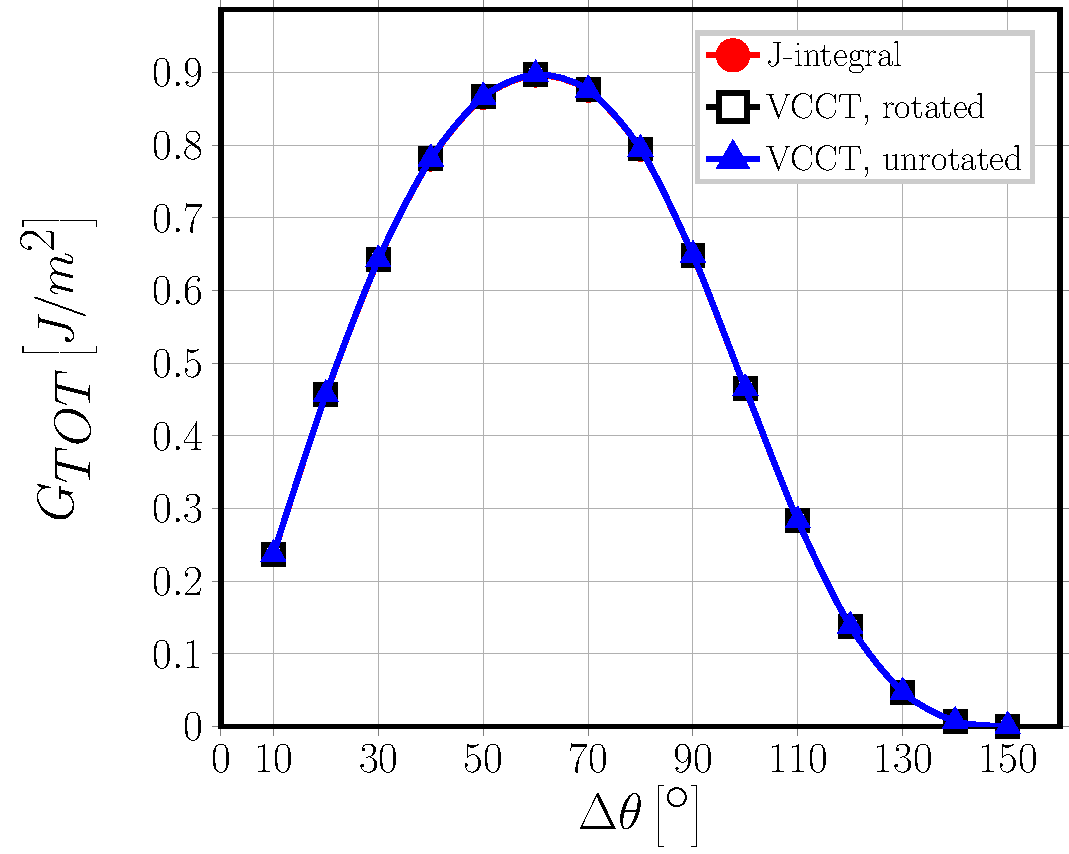
\includegraphics[width=\textwidth]{paperA/Vf0_1-free-1st-05-invrot-GTOT.pdf}
       \caption{$V_{f}=0.1\%$, $1^{st}$ order elements, $\delta=0.05^{\circ}$.}
    \end{subfigure}
    ~
    \begin{subfigure}[b]{0.48\textwidth}
        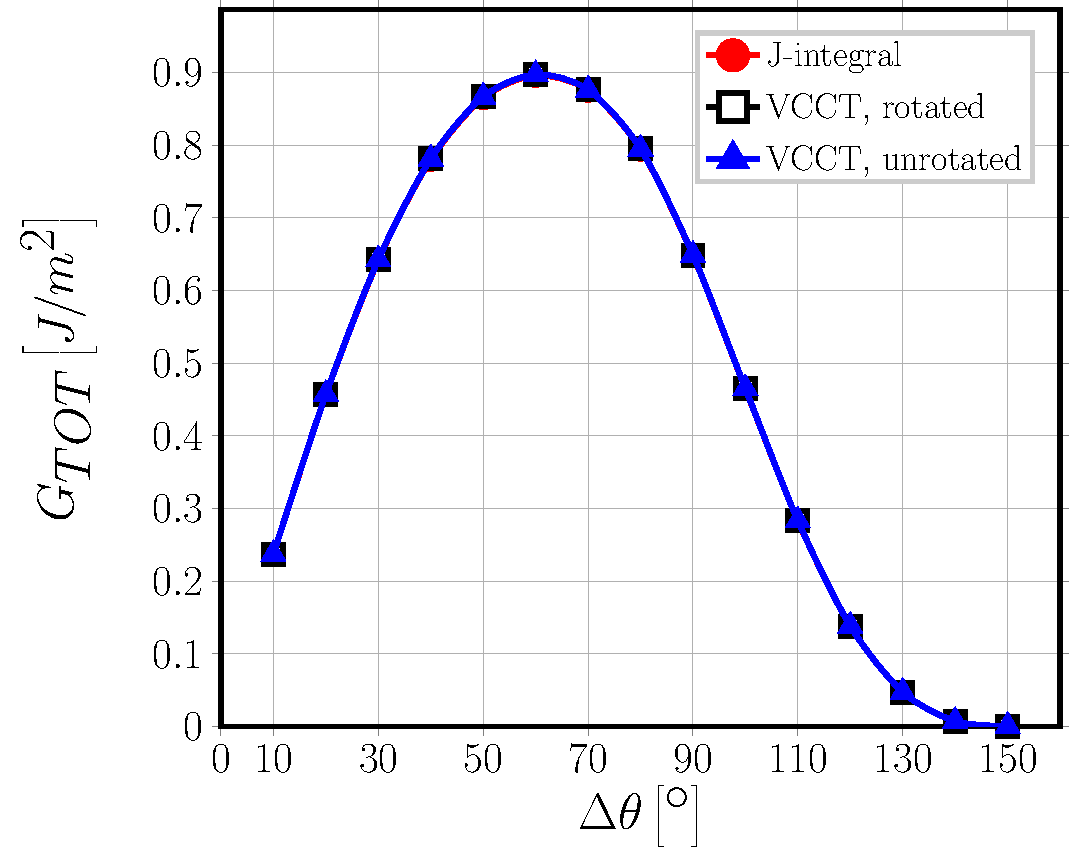
\includegraphics[width=\textwidth]{paperA/Vf0_1-free-2nd-05-invrot-GTOT.pdf}
       \caption{$V_{f}=0.1\%$, $2^{nd}$ order elements, $\delta=0.05^{\circ}$.}
    \end{subfigure}

    \begin{subfigure}[b]{0.48\textwidth}
        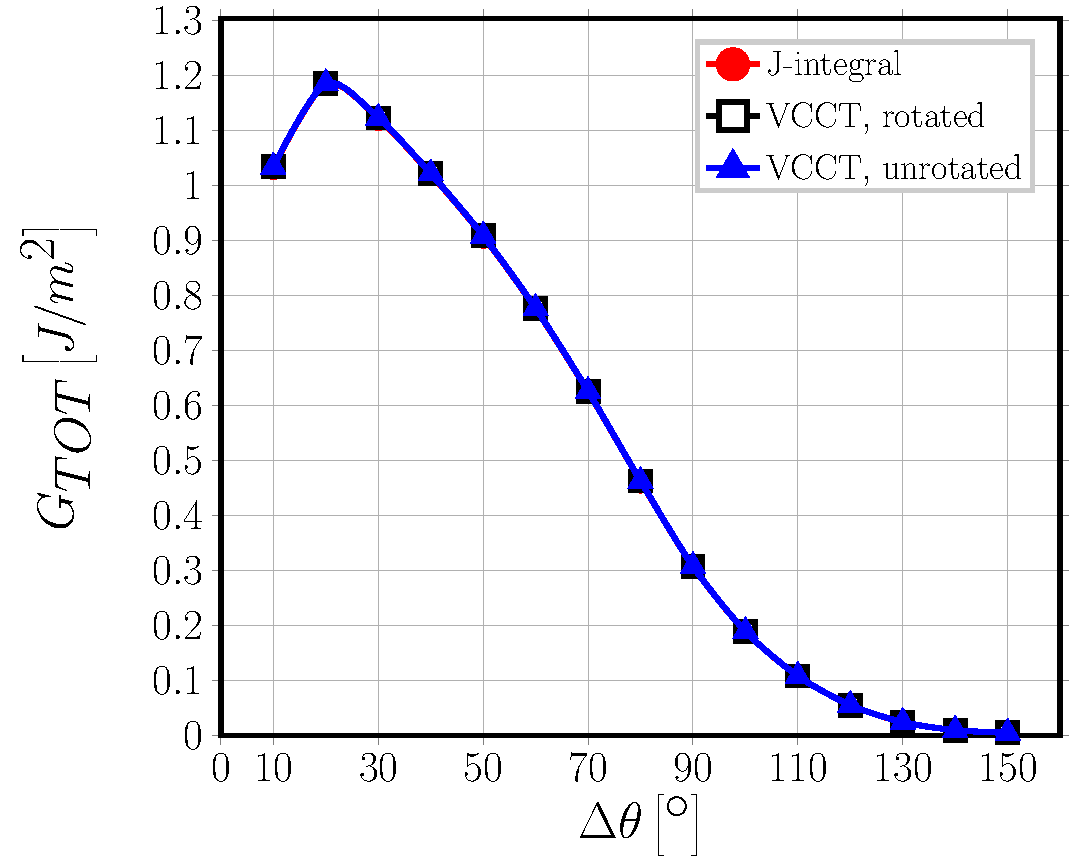
\includegraphics[width=\textwidth]{paperA/Vf40-free-1st-05-invrot-GTOT.pdf}
       \caption{$V_{f}=40\%$, $1^{st}$ order elements, $\delta=0.05^{\circ}$.}
    \end{subfigure}
    ~
    \begin{subfigure}[b]{0.48\textwidth}
        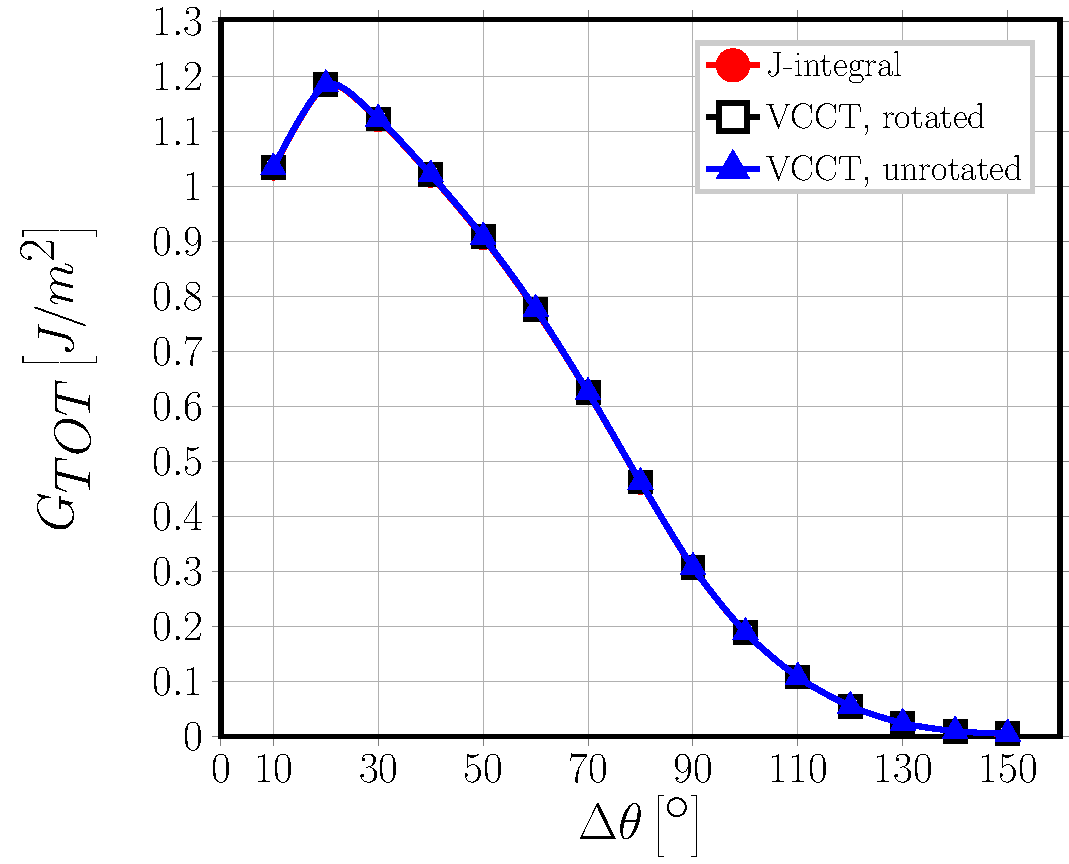
\includegraphics[width=\textwidth]{paperA/Vf40-free-2nd-05-invrot-GTOT.pdf}
       \caption{$V_{f}=40\%$, $2^{nd}$ order elements, $\delta=0.05^{\circ}$ .}
    \end{subfigure}

\caption{Numerical invariance of the total Energy Release Rate: $G_{TOT}$ computed with the VCCT with rotated forces and displacements (label \emph{rotated}), with the VCCT with forces and displacements in the global reference frame (label \emph{unrotated}) and with J-integral method (label \emph{J-integral}).}\label{paperA:fig:gtotrotinvnum}
\end{figure}

The result of Equation~\ref{paperA:eq:gtotrotinv} has also physical implications:

\begin{itemize}[label={--}]
\item given that stress and displacement fields at the crack tip are the same, two cracks with different crack paths are energetically equivalent with respect to the total Energy Release Rate;
\item given that laws of the type $G_{TOT}\geq G_{c}$ govern crack propagation, if $G_{c}$ do not depend on mode ratio, crack orientation will not affect its growth.
\end{itemize}

\section{Convergence analysis}

\subsection{Analytical considerations}

Substituting Equations~\ref{paperA:eq:rotmatdev} in the derivative of Equation~\ref{paperA:eq:g}, we can investigate the dependency of Mode I and Mode II ERR with respect to the size $\delta$ of an element in the crack tip neighborhood through

\begin{equation}
\scriptsize
\begin{split}
\frac{\partial \underline{G}}{\partial \delta}=&-\frac{1}{2R_{f}\delta^{2}}\sum_{p=1}^{m+1}\sum_{q=1}^{m+1}Diag\left(\underline{\underline{Q}}_{\delta}\underline{\underline{R}}_{\Delta\theta}\underline{\underline{K}}_{xy}\underline{u}_{xy}\underline{u}_{xy}^{T}\underline{\underline{R}}_{\Delta\theta}^{T}\underline{\underline{P}}_{\delta}^{T}\underline{\underline{T}}_{pq}^{T}\right)-\frac{1}{2R_{f}\delta^{2}}\sum_{p=1}^{m+1}\sum_{q=1}^{m+1}Diag\left(\underline{\underline{Q}}_{\delta}\underline{\underline{R}}_{\Delta\theta}\underline{\underline{\widetilde{K}}}_{N}\underline{u}_{N}\underline{u}_{xy}^{T}\underline{\underline{R}}_{\Delta\theta}^{T}\underline{\underline{P}}_{\delta}^{T}\underline{\underline{T}}_{pq}^{T}\right)+\\
+&\frac{1}{2R_{f}\delta}\sum_{p=1}^{m+1}\sum_{q=1}^{m+1}Diag\left(\underline{\underline{Q}}_{\delta}\underline{\underline{R}}_{\Delta\theta}\underline{\underline{K}}_{xy}\underline{u}_{xy}\underline{u}_{xy}^{T}\underline{\underline{R}}_{\Delta\theta}^{T}\underline{\underline{P}}_{\delta}^{T}\underline{\underline{D}}^{T}\underline{\underline{T}}_{pq}^{T}\right)+\frac{1}{2R_{f}\delta}\sum_{p=1}^{m+1}\sum_{q=1}^{m+1}Diag\left(\underline{\underline{Q}}_{\delta}\underline{\underline{R}}_{\Delta\theta}\underline{\underline{\widetilde{K}}}_{N}\underline{u}_{N}\underline{u}_{xy}^{T}\underline{\underline{R}}_{\Delta\theta}^{T}\underline{\underline{P}}_{\delta}^{T}\underline{\underline{D}}^{T}\underline{\underline{T}}_{pq}^{T}\right)+\\
+&\frac{1}{2R_{f}\delta}\sum_{p=1}^{m+1}\sum_{q=1}^{m+1}Diag\left(\underline{\underline{D}}\underline{\underline{Q}}_{\delta}\underline{\underline{R}}_{\Delta\theta}\underline{\underline{K}}_{xy}\underline{u}_{xy}\underline{u}_{xy}^{T}\underline{\underline{R}}_{\Delta\theta}^{T}\underline{\underline{P}}_{\delta}^{T}\underline{\underline{T}}_{pq}^{T}\right)+\frac{1}{2R_{f}\delta}\sum_{p=1}^{m+1}\sum_{q=1}^{m+1}Diag\left(\underline{\underline{D}}\underline{\underline{Q}}_{\delta}\underline{\underline{R}}_{\Delta\theta}\underline{\underline{\widetilde{K}}}_{N}\underline{u}_{N}\underline{u}_{xy}^{T}\underline{\underline{R}}_{\Delta\theta}^{T}\underline{\underline{P}}_{\delta}^{T}\underline{\underline{T}}_{pq}^{T}\right)+\\
+&\frac{1}{2R_{f}\delta}\sum_{p=1}^{m+1}\sum_{q=1}^{m+1}Diag\left(\underline{\underline{Q}}_{\delta}\underline{\underline{R}}_{\Delta\theta}\underline{\underline{K}}_{xy}\frac{\partial \underline{u}_{xy}}{\partial \delta}\underline{u}_{xy}^{T}\underline{\underline{R}}_{\Delta\theta}^{T}\underline{\underline{P}}_{\delta}^{T}\underline{\underline{T}}_{pq}^{T}\right)+\frac{1}{2R_{f}\delta}\sum_{p=1}^{m+1}\sum_{q=1}^{m+1}Diag\left(\underline{\underline{Q}}_{\delta}\underline{\underline{R}}_{\Delta\theta}\underline{\underline{\widetilde{K}}}_{N}\frac{\partial \underline{u}_{N}}{\partial \delta}\underline{u}_{xy}^{T}\underline{\underline{R}}_{\Delta\theta}^{T}\underline{\underline{P}}_{\delta}^{T}\underline{\underline{T}}_{pq}^{T}\right)+\\
+&\frac{1}{2R_{f}\delta}\sum_{p=1}^{m+1}\sum_{q=1}^{m+1}Diag\left(\underline{\underline{Q}}_{\delta}\underline{\underline{R}}_{\Delta\theta}\underline{\underline{K}}_{xy}\underline{u}_{xy}\frac{\partial \underline{u}_{xy}^{T}}{\partial \delta}\underline{\underline{R}}_{\Delta\theta}^{T}\underline{\underline{P}}_{\delta}^{T}\underline{\underline{T}}_{pq}^{T}\right)+\frac{1}{2R_{f}\delta}\sum_{p=1}^{m+1}\sum_{q=1}^{m+1}Diag\left(\underline{\underline{Q}}_{\delta}\underline{\underline{R}}_{\Delta\theta}\underline{\underline{\widetilde{K}}}_{N}\underline{u}_{N}\frac{\partial \underline{u}_{xy}^{T}}{\partial \delta}\underline{\underline{R}}_{\Delta\theta}^{T}\underline{\underline{P}}_{\delta}^{T}\underline{\underline{T}}_{pq}^{T}\right);
\end{split}
\end{equation}

which, after refactoring, provides

\begin{equation}\label{paperA:eq:Gdev}
\scriptsize
\begin{split}
\frac{\partial \underline{G}}{\partial \delta}=&\frac{1}{\delta}\underline{G}+\frac{1}{2R_{f}\delta}\sum_{p=1}^{m+1}\sum_{q=1}^{m+1}Diag\left(\underline{\underline{Q}}_{\delta}\underline{\underline{R}}_{\Delta\theta}\left(\underline{\underline{K}}_{xy}\underline{u}_{xy}+\underline{\underline{\widetilde{K}}}_{N}\underline{u}_{N}\right)\underline{u}_{xy}^{T}\underline{\underline{R}}_{\Delta\theta}^{T}\underline{\underline{P}}_{\delta}^{T}\underline{\underline{D}}^{T}\underline{\underline{T}}_{pq}^{T}\right)+\\
+&\frac{1}{2R_{f}\delta}\sum_{p=1}^{m+1}\sum_{q=1}^{m+1}Diag\left(\underline{\underline{D}}\underline{\underline{Q}}_{\delta}\underline{\underline{R}}_{\Delta\theta}\left(\underline{\underline{K}}_{xy}\underline{u}_{xy}+\underline{\underline{\widetilde{K}}}_{N}\underline{u}_{N}\right)\underline{u}_{xy}^{T}\underline{\underline{R}}_{\Delta\theta}^{T}\underline{\underline{P}}_{\delta}^{T}\underline{\underline{T}}_{pq}^{T}\right)+\\
+&\frac{1}{R_{f}\delta}\sum_{p=1}^{m+1}\sum_{q=1}^{m+1}Diag\left(\underline{\underline{Q}}_{\delta}\underline{\underline{R}}_{\Delta\theta}\underline{\underline{K}}_{xy}\frac{\partial \underline{u}_{xy}}{\partial \delta}\underline{u}_{xy}^{T}\underline{\underline{R}}_{\Delta\theta}^{T}\underline{\underline{P}}_{\delta}^{T}\underline{\underline{T}}_{pq}^{T}\right)+\frac{1}{2R_{f}\delta}\sum_{p=1}^{m+1}\sum_{q=1}^{m+1}Diag\left(\underline{\underline{Q}}_{\delta}\underline{\underline{R}}_{\Delta\theta}\underline{\underline{\widetilde{K}}}_{N}\frac{\partial \underline{u}_{N}}{\partial \delta}\underline{u}_{xy}^{T}\underline{\underline{R}}_{\Delta\theta}^{T}\underline{\underline{P}}_{\delta}^{T}\underline{\underline{T}}_{pq}^{T}\right)+\\
+&\frac{1}{2R_{f}\delta}\sum_{p=1}^{m+1}\sum_{q=1}^{m+1}Diag\left(\underline{\underline{Q}}_{\delta}\underline{\underline{R}}_{\Delta\theta}\underline{\underline{\widetilde{K}}}_{N}\underline{u}_{N}\frac{\partial \underline{u}_{xy}^{T}}{\partial \delta}\underline{\underline{R}}_{\Delta\theta}^{T}\underline{\underline{P}}_{\delta}^{T}\underline{\underline{T}}_{pq}^{T}\right).
\end{split}
\end{equation}

Following the asymptotic analysis of~\cite{Williams1959,Comninou1990}, in the case of an \emph{open crack} the displacement in the crack tip neighborhood will have a functional form of the type

\begin{equation}\label{paperA:eq:basicasymptotic}
u\left(\delta\right)\sim \sqrt{\delta}\left(\sin,\cos\right)\left(\epsilon\log{\delta}\right)\quad\text{with}\quad\epsilon=\frac{1}{2\pi}\log{\left(\frac{1-\beta}{1+\beta}\right)}
\end{equation}

and $\beta$ is Dundurs' parameter introduced in Section~\ref{paperA:sec:intro}. Application of Equation~\ref{paperA:eq:basicasymptotic} to the terms on the right hand side of Eq.~\ref{paperA:eq:Gdev} provides:

\begin{equation}\label{paperA:eq:asym1}
\underline{u}_{xy},\underline{u}_{N}\sim u\left(\delta\right)\sim\sqrt{\delta}\left(\sin,\cos\right)\left(\epsilon\log{\delta}\right)\xrightarrow{\delta\rightarrow 0}0;
\end{equation}

\begin{equation}\label{paperA:eq:asym2}
\underline{u}_{xy}\underline{u}_{xy}^{T},\underline{u}_{N}\underline{u}_{xy}^{T}\sim u^{2}\left(\delta\right)\sim\delta\left(\sin^{2},\cos^{2},\sin\cdot\cos\right)\left(\epsilon\log{\delta}\right)\xrightarrow{\delta\rightarrow 0}0;
\end{equation}

\begin{equation}\label{paperA:eq:asym3}
\frac{\partial \underline{u}_{xy}}{\partial \delta}\underline{u}_{xy}^{T},\frac{\partial \underline{u}_{N}}{\partial \delta}\underline{u}_{xy}^{T}\sim -\frac{1}{2}\left(\sin^{2},\cos^{2},\sin\cdot\cos\right)\left(\epsilon\log{\delta}\right)+\left(-\sin^{2},\cos^{2},\pm\sin\cdot\cos\right)\left(\epsilon\log{\delta}\right)\xrightarrow{\delta\rightarrow 0}finite;
\end{equation}

\begin{equation}\label{paperA:eq:asym4}
\underline{G}\sim\frac{1}{\delta}\underline{u}_{xy}\underline{u}_{xy}^{T}\sim \frac{1}{\delta}u^{2}\left(\delta\right)\sim\left(\sin^{2},\cos^{2},\sin\cdot\cos\right)\left(\epsilon\log{\delta}\right)\xrightarrow{\delta\rightarrow 0}finite.
\end{equation}

In Equations~\ref{paperA:eq:asym1}-\ref{paperA:eq:asym4}, the multiplication by a trigonometric function of the type $\left(\sin,\cos,\sin^{2},\cos^{2},\sin\cdot\cos\right)$ prevents the divergence of the asymptote. Recalling Eqs.~\ref{paperA:eq:Pmatrix} and~\ref{paperA:eq:Qmatrix}, in the limit of $\delta\rightarrow 0$ the rotation matrices become equal to the identity matrix:

\begin{equation}\label{paperA:eq:PQasym}
\underline{\underline{P}}_{\delta},\underline{\underline{Q}}_{\delta}\xrightarrow{\delta\rightarrow 0}\begin{bmatrix}1&0\\0&1\end{bmatrix}.
\end{equation}

Applying the results of Equations~\ref{paperA:eq:asym1}-\ref{paperA:eq:PQasym} to Eq.~\ref{paperA:eq:Gdev}, it can be shown that the derivative of $\underline{G}$ can be split in a factor that goes to $0$ in the limit of $\delta\rightarrow 0$ and in a factor independent of $\delta$:

\begin{equation}
\lim_{\delta\rightarrow 0}\frac{\partial \underline{G}}{\partial \delta}\sim\frac{1}{\delta}\left(\cancelto{0}{\underline{F}\left(\delta\right)}+\underline{C}\right).
\end{equation}

Thus, asymptotically, the Mode I and Mode II Energy Release Rate behave like the logarithm of the angular size $\delta$ of the elements in the crack tip neighborhood:

\begin{equation}
\lim_{\delta\rightarrow 0}\frac{\partial \underline{G}}{\partial \delta}\sim\frac{1}{\delta}\quad\xrightarrow{\int d\delta}\quad\lim_{\delta\rightarrow 0}\underline{G}\sim \underline{A}\log(\delta)+\underline{B}.
\end{equation}

\subsection{Numerical results}

Evaluations of the Mode I, Mode II and total Energy Release Rate using the VCCT applied to the FE solution of the fiber-matrix interface crack in the single fiber model of Sec.~\ref{paperA:sec:femmodel} are reported respectively in Fig.~\ref{paperA:fig:ginum}, Fig.~\ref{paperA:fig:giinum} and Fig.~\ref{paperA:fig:gtotnum}.

\begin{figure}[!h]
\centering
    \begin{subfigure}[b]{0.48\textwidth}
        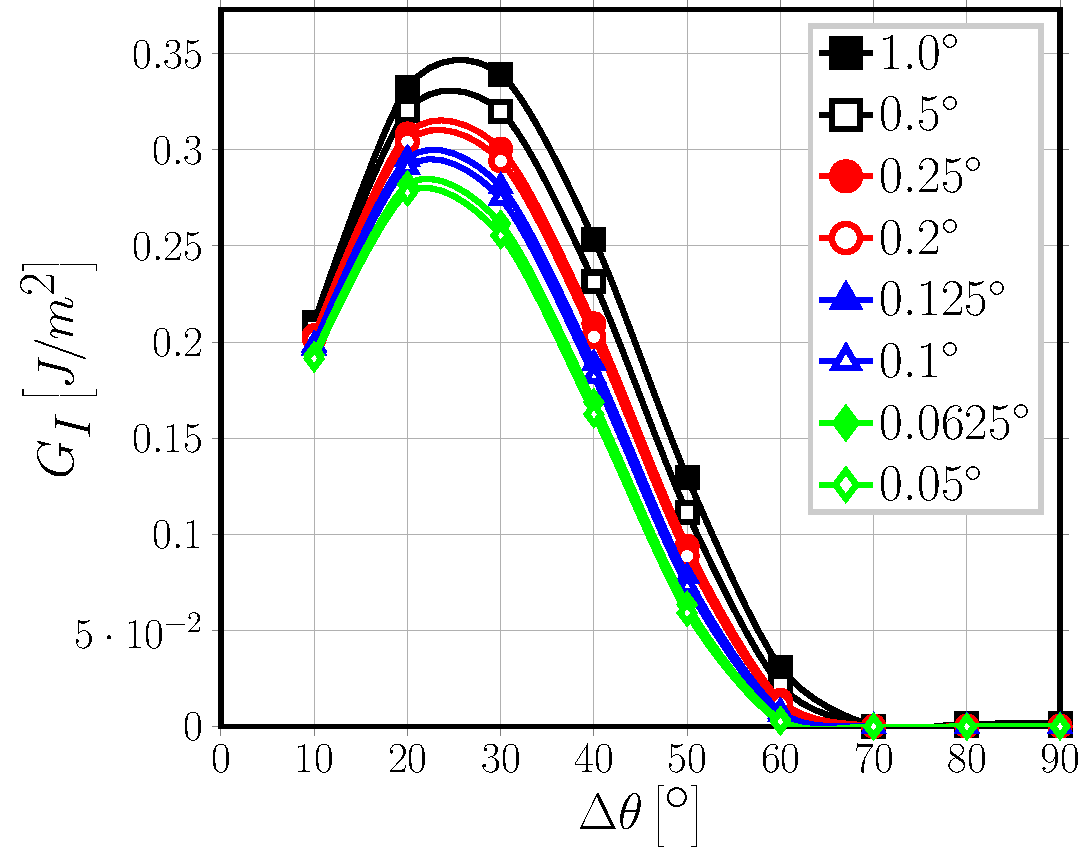
\includegraphics[width=\textwidth]{paperA/Vf0_1-free-1st-GI.pdf}
       \caption{$V_{f}=0.1\%$, $1^{st}$ order elements.}
    \end{subfigure}
    ~
    \begin{subfigure}[b]{0.48\textwidth}
        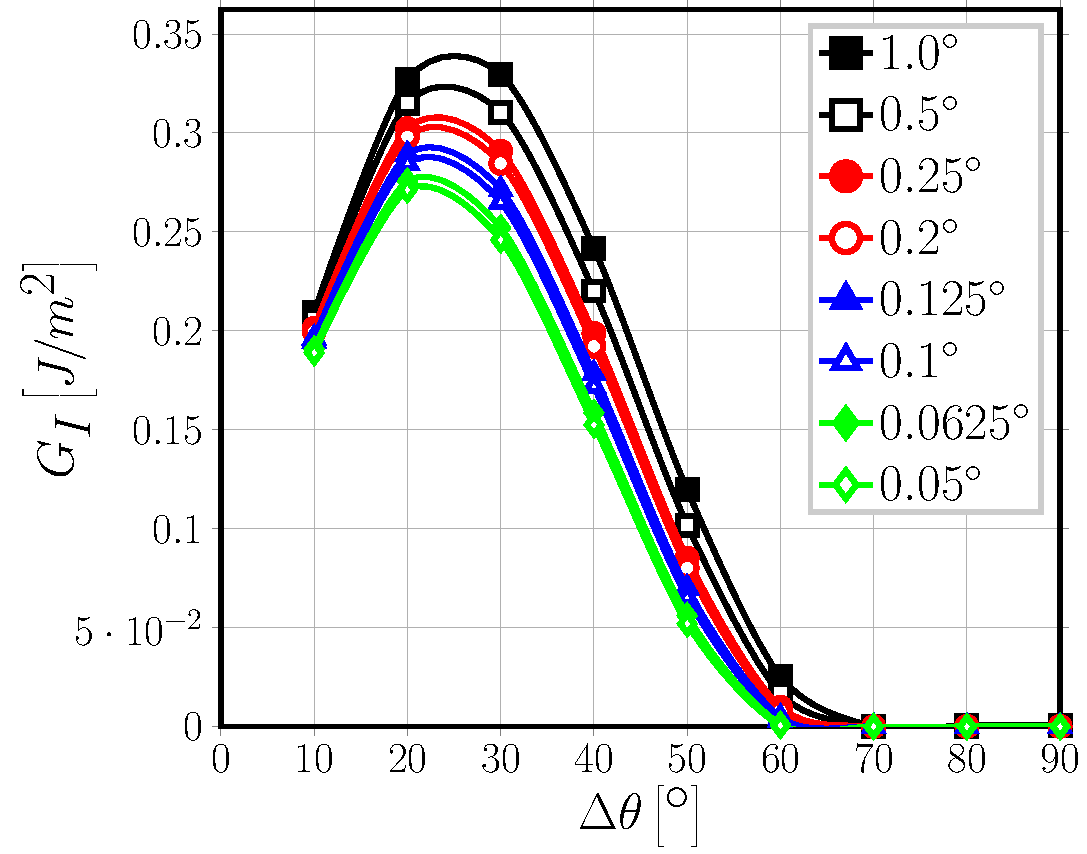
\includegraphics[width=\textwidth]{paperA/Vf0_1-free-2nd-GI.pdf}
       \caption{$V_{f}=0.1\%$, $2^{nd}$ order elements.}
    \end{subfigure}

    \begin{subfigure}[b]{0.48\textwidth}
        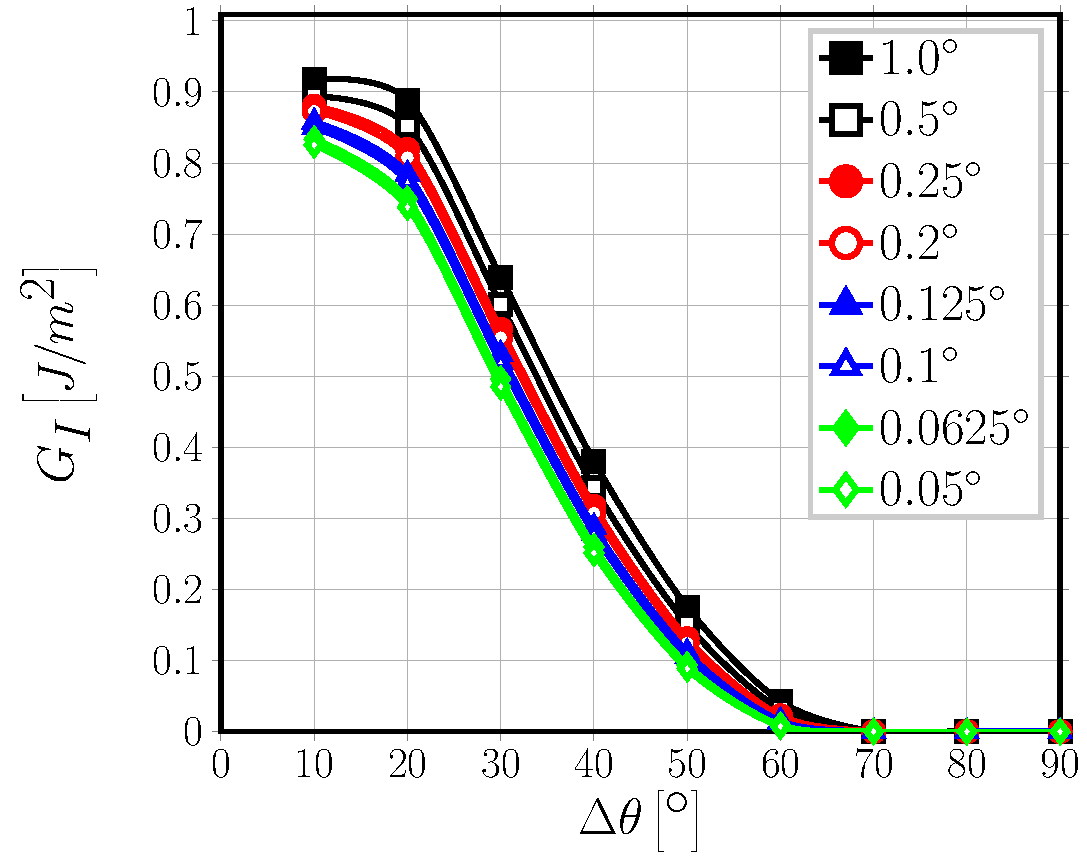
\includegraphics[width=\textwidth]{paperA/Vf40-free-1st-GI.pdf}
       \caption{$V_{f}=40\%$, $1^{st}$ order elements.}
    \end{subfigure}
    ~
    \begin{subfigure}[b]{0.48\textwidth}
        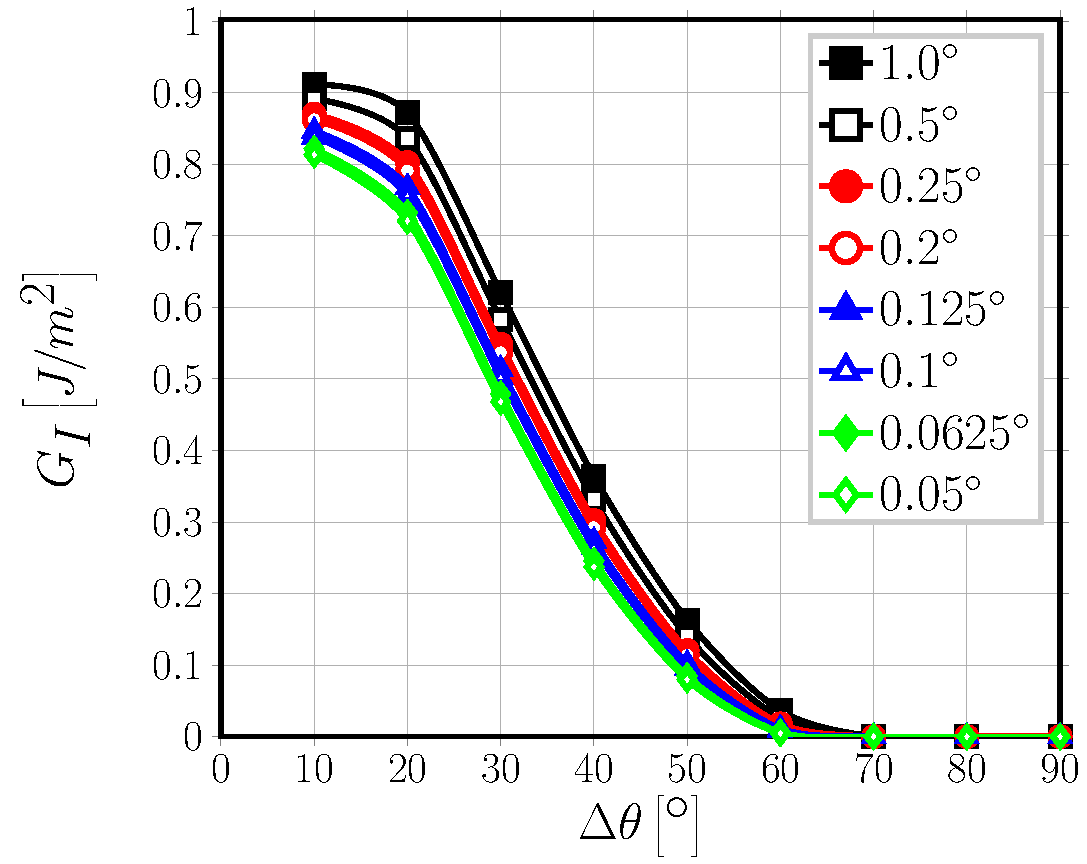
\includegraphics[width=\textwidth]{paperA/Vf40-free-2nd-GI.pdf}
       \caption{$V_{f}=40\%$, $2^{nd}$ order elements.}
    \end{subfigure}

\caption{Effect of the size $\delta$ of an element at the crack tip on Mode I ERR.}\label{paperA:fig:ginum}
\end{figure}

Results for Mode I ERR in Fig.~\ref{paperA:fig:ginum} show clearly the transition from the \emph{open} crack regime, where Mode I ERR is different from zero, to the \emph{closed} crack regime of the debond, where $G_{I}=0$. Looking at Fig.~\ref{paperA:fig:ginum}, the crack is \emph{open} for $\Delta\theta\leq60^{\circ}$ and it is \emph{closed}, i.e. a contact zone is present, for $\Delta\theta\geq70^{\circ}$. As expected from the analysis of the previous section, and given that Mode I ERR is different from zero only in the \emph{open} crack regime, a significant dependence on the element size $\delta$ can be observed in  Fig.~\ref{paperA:fig:ginum} when using both $1^{st}$ and $2^{nd}$ order elements and with both an effectively infinite ($V_{f}=0.1\%$) and finite size ($V_{f}=40\%$) matrix. At first sight, it is immediate to see from Fig.~\ref{paperA:fig:ginum} that a decrease in $\delta$ leads to a decrease in $G_{I}$. However, two further effects can be observed due to the refinement of the mesh at the crack tip, i.e. the decrease of the element size $\delta$. First, the occurrence of the peak $G_{I}$ is shifted to lower angles for very low volume fractions: it occurs at $\Delta\theta=30^{\circ}$ with $\delta=1.0^{\circ}, 0.5^{\circ}$ and at $\Delta\theta=20^{\circ}$ with $\delta\leq0.25^{\circ}$ for both $1^{st}$ and $2^{nd}$ order elements and $V_{f}=0.1\%$. Second, the apperance of the contact zone, i.e. the switch to the \emph{closed} crack regime, is anticipated to smaller debonds: it occurs at  $\Delta\theta=70^{\circ}$ with $\delta\geq0.2^{\circ}$ and at $\Delta\theta=60^{\circ}$ with $\delta<0.2^{\circ}$ for both $1^{st}$ and $2^{nd}$ order elements and both $V_{f}=0.1\%$ and $V_{f}=40\%$.

\begin{figure}[!h]
\centering
    \begin{subfigure}[b]{0.48\textwidth}
        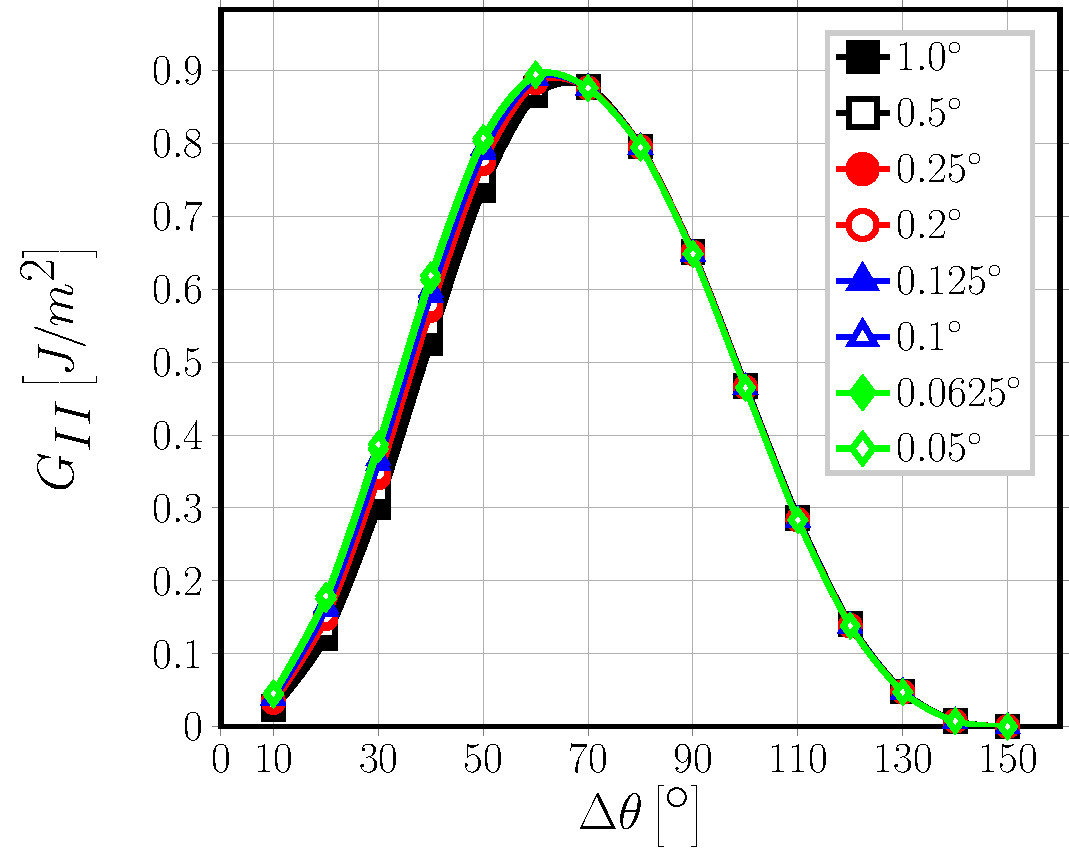
\includegraphics[width=\textwidth]{paperA/Vf0_1-free-1st-GII.pdf}
       \caption{$V_{f}=0.1\%$, $1^{st}$ order elements.}
    \end{subfigure}
    ~
    \begin{subfigure}[b]{0.48\textwidth}
        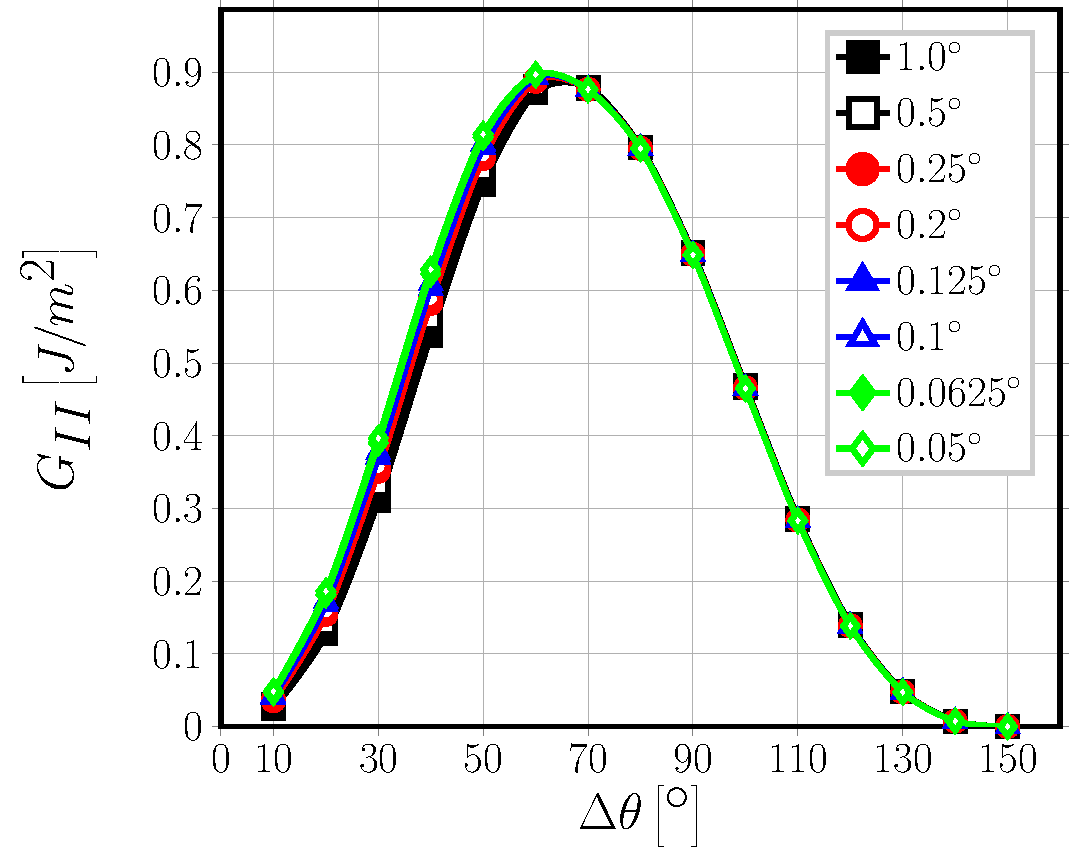
\includegraphics[width=\textwidth]{paperA/Vf0_1-free-2nd-GII.pdf}
       \caption{$V_{f}=0.1\%$, $2^{nd}$ order elements.}
    \end{subfigure}

    \begin{subfigure}[b]{0.48\textwidth}
        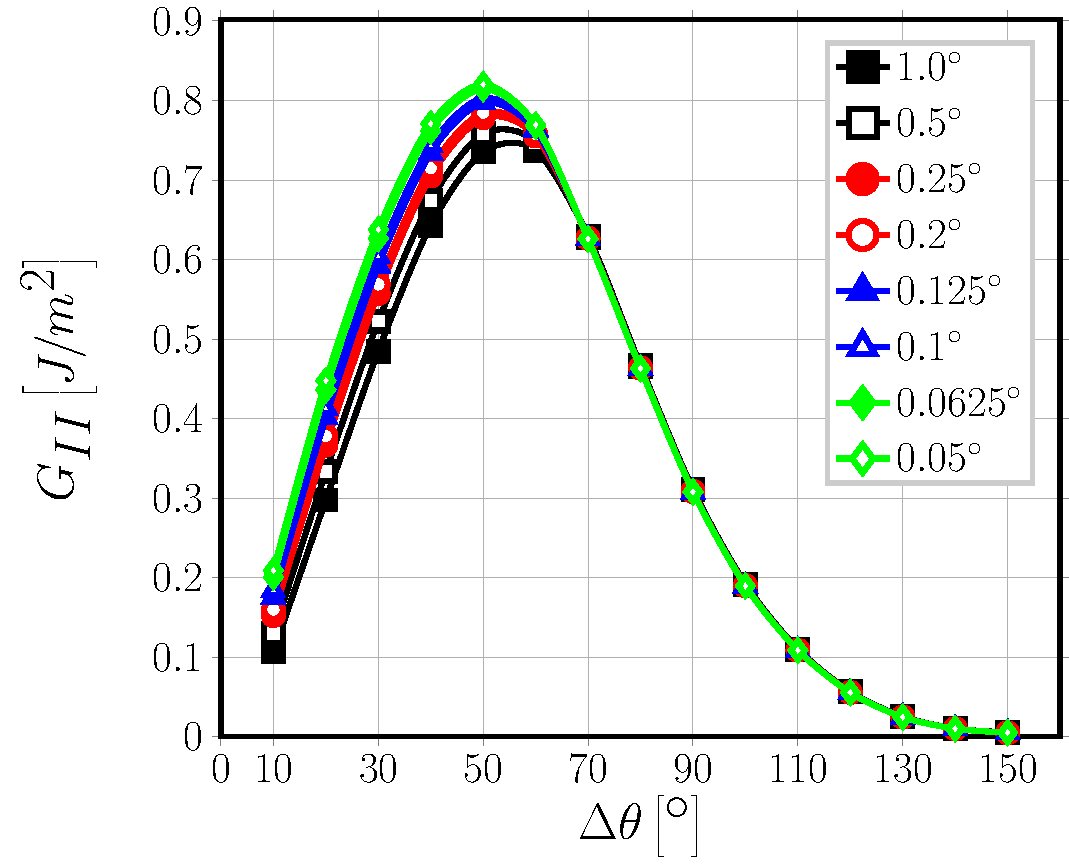
\includegraphics[width=\textwidth]{paperA/Vf40-free-1st-GII.pdf}
       \caption{$V_{f}=40\%$, $1^{st}$ order elements.}
    \end{subfigure}
    ~
    \begin{subfigure}[b]{0.48\textwidth}
        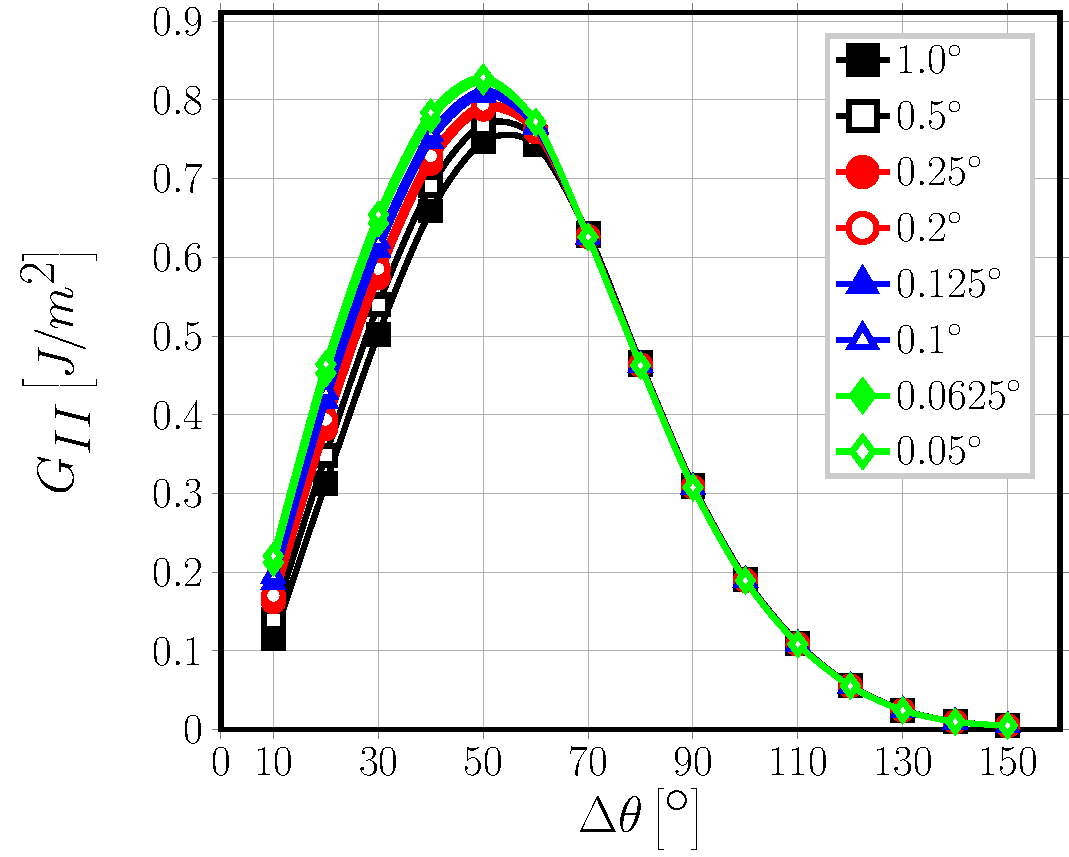
\includegraphics[width=\textwidth]{paperA/Vf40-free-2nd-GII.pdf}
       \caption{$V_{f}=40\%$, $2^{nd}$ order elements.}
    \end{subfigure}

\caption{Effect of the size $\delta$ of an element at the crack tip on Mode II ERR.}\label{paperA:fig:giinum}
\end{figure}

Observing Figure~\ref{paperA:fig:giinum}, it possible to notice the existence of two distinct regimes in the behavior of $G_{II}$ with respect to the element size $\delta$. For $\Delta\theta\leq60^{\circ}$ $G_{II}$ depends on the value of $\delta$, while $\Delta\theta\geq70^{\circ}$ it is effectively independent of the element size at the crack tip for both $1^{st}$ and $2^{nd}$ order elements and both an effectively infinite ($V_{f}=0.1\%$) and finite size ($V_{f}=40\%$) matrix. Comparing the value of $\Delta\theta$ at which the change from the $\delta$-dependency regime to the $\delta$-independency regime occurs for $G_{II}$ with Mode I ERR in Fig.~\ref{paperA:fig:ginum}, it is possible to observe that the $\delta$-dependency regime change of Mode II ERR coincides with the onset of the contact zone, i.e. the transition from \emph{open} crack regime to the \emph{closed} crack regime. The result confirms the analytical considerations of the previous section: for an \emph{open} crack both Mode I and Mode II ERR depend on the element size $\delta$ at the crack tip.

\begin{figure}[!h]
\centering
    \begin{subfigure}[b]{0.48\textwidth}
        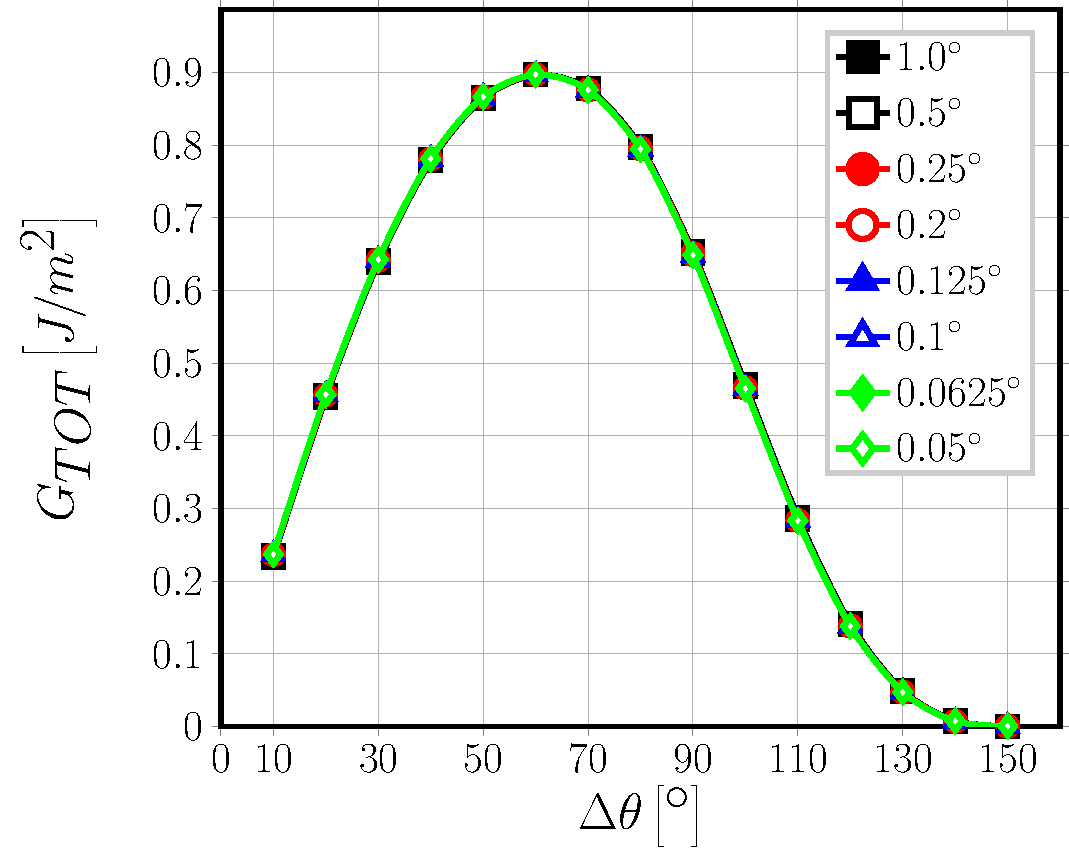
\includegraphics[width=\textwidth]{paperA/Vf0_1-free-1st-GTOT.pdf}
       \caption{$V_{f}=0.1\%$, $1^{st}$ order elements.}
    \end{subfigure}
    ~
    \begin{subfigure}[b]{0.48\textwidth}
        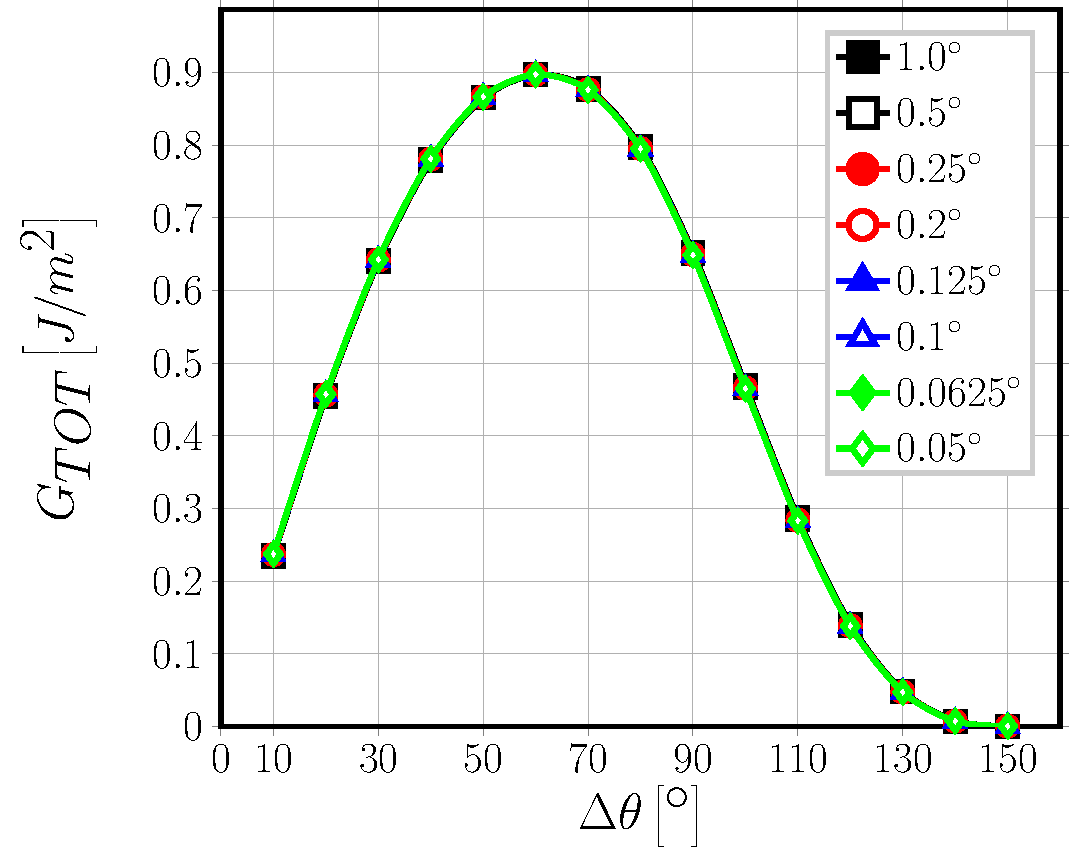
\includegraphics[width=\textwidth]{paperA/Vf0_1-free-2nd-GTOT.pdf}
       \caption{$V_{f}=0.1\%$, $2^{nd}$ order elements.}
    \end{subfigure}

    \begin{subfigure}[b]{0.48\textwidth}
        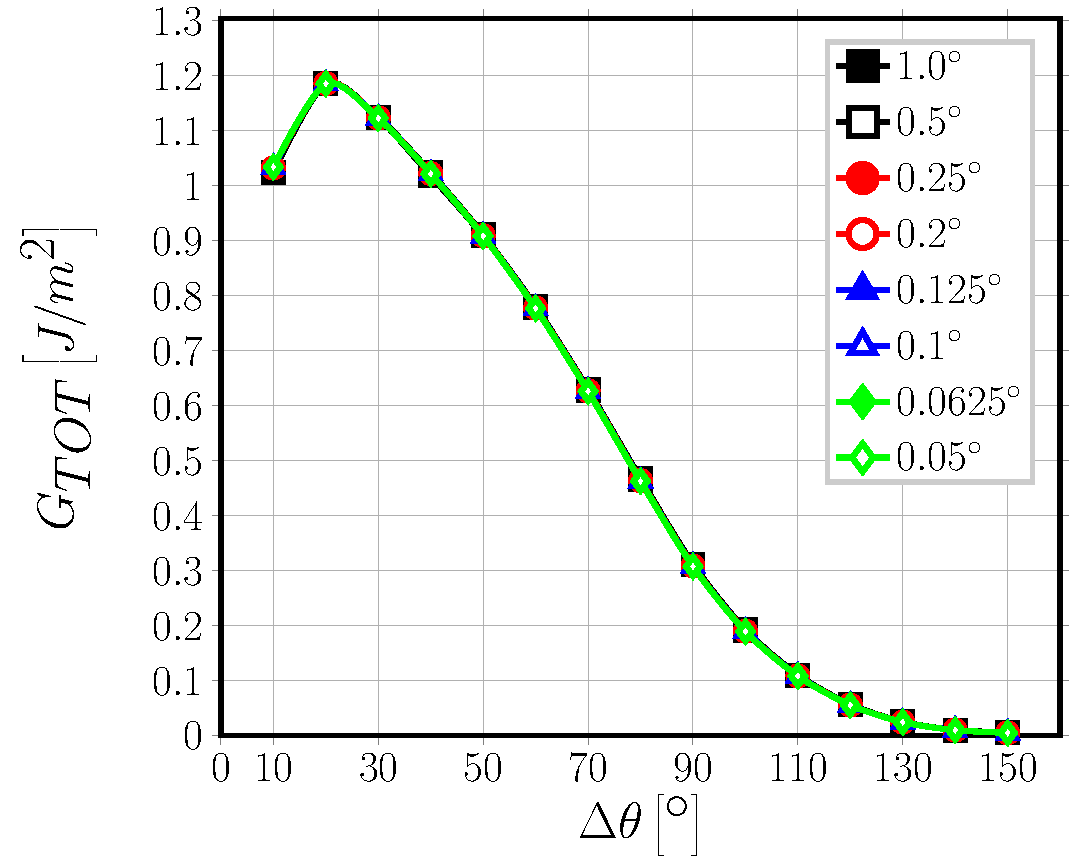
\includegraphics[width=\textwidth]{paperA/Vf40-free-1st-GTOT.pdf}
       \caption{$V_{f}=40\%$, $1^{st}$ order elements.}
    \end{subfigure}
    ~
    \begin{subfigure}[b]{0.48\textwidth}
        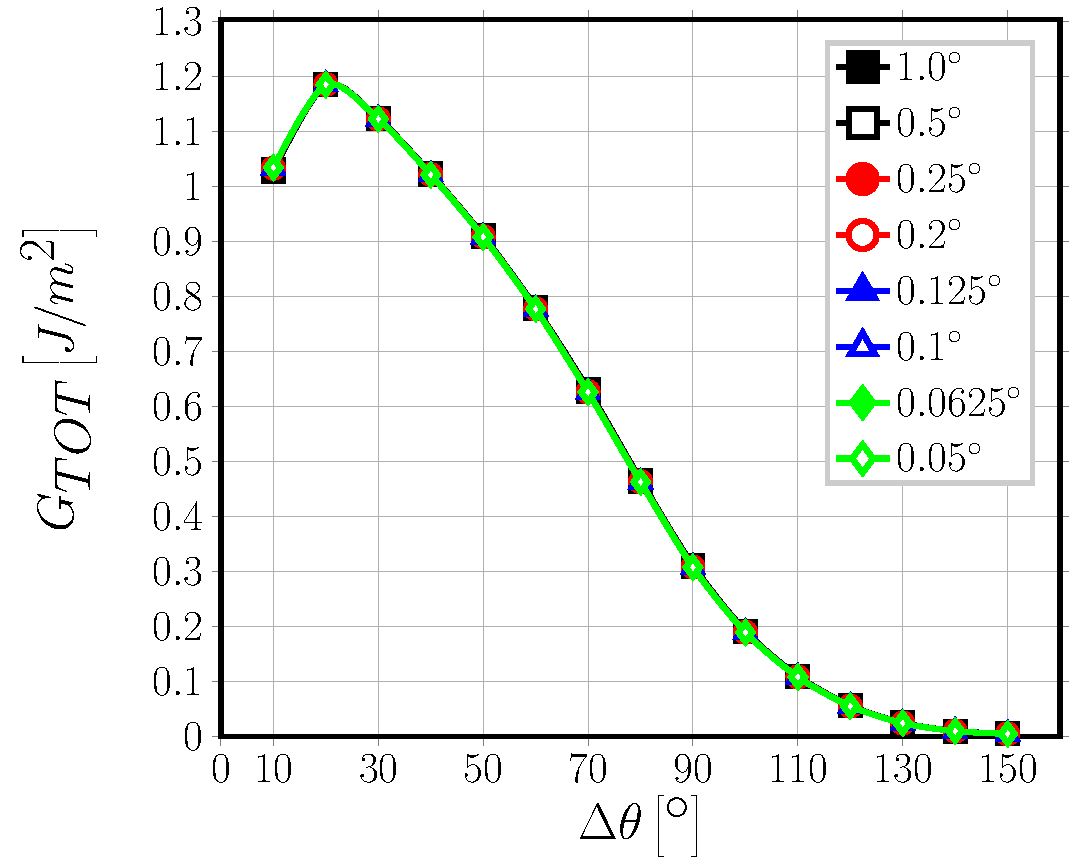
\includegraphics[width=\textwidth]{paperA/Vf40-free-2nd-GTOT.pdf}
       \caption{$V_{f}=40\%$, $2^{nd}$ order elements.}
    \end{subfigure}

\caption{Effect of the size $\delta$ of an element at the crack tip on total ERR.}\label{paperA:fig:gtotnum}
\end{figure}

Further observation of Figure~\ref{paperA:fig:giinum} reveals that, in the \emph{open} crack regime, decreasing the element size $\delta$ causes an increase of Mode II ERR. Similarly to Mode I ERR, a shift of the peak $G_{II}$ can also observed for $V_{f}=0.1\%$: the maximum value of $G_{II}$ occurs at $\Delta\theta=70^{\circ}$ for $\delta>0.25^{\circ}$ for $1^{st}$ order elements and for $\delta>0.5^{\circ}$ for $2^{nd}$ order elements, while it is shifted to $\Delta\theta=60^{\circ}$ for $\delta\leq0.25^{\circ}$ for $1^{st}$ order elements and for $\delta\leq0.5^{\circ}$ for $2^{nd}$ order elements.

\begin{table}[!h]
 \centering
 \caption{Summary of linear regression results and main statistical tests for Mode I ERR}\label{paperA:tab:GIinterp}
 \begin{tabular}{ccccccccc}
\small$\mathbf{V_{f} \left[\%\right]}$&\small\bf{Order}&\small$\mathbf{\Delta\theta \left[^{\circ}\right]}$&\small$\mathbf{A\left[\frac{J}{m^{2}}\right]}$ &\small$\mathbf{B\left[\frac{J}{m^{2}}\right]}$ &\small $\mathbf{r\left[-\right]}$ &\small $\mathbf{r^{2}\left[-\right]}$ &\small $\mathbf{p(A)\left[-\right]}$ &\small $\mathbf{p(B)\left[-\right]}$\\
\toprule
\midrule
\small0.1&\small1&	\small10.0&	\small0.0064&	\small0.2113&	\small0.9933&	\small0.9866&	\small7.48E-07&	\small3.49E-14\\
&&		\small20.0& \small0.0183&\small	0.3331&\small	0.9996&\small	0.9992&\small	1.44E-10&\small	2.40E-16\\
&&		\small30.0&	\small0.0280&\small	0.3392&\small	1.0000&\small	1.0000&\small	2.25E-16&\small	4.26E-21\\
&&		\small40.0&	\small0.0304&\small	0.2524&\small	0.9997&\small	0.9995&\small	4.38E-11&\small	7.94E-15\\
&&		\small50.0&	\small0.0235&\small	0.1278&\small	0.9985&\small	0.9970&\small	8.61E-09&\small	2.01E-11\\
&&		\small60.0&	\small0.0094&\small	0.0284&\small	0.9854&\small	0.9709&\small	7.75E-06&\small	6.14E-07\\
\midrule
\small0.1&\small2&	\small10.0&	\small0.0069&	\small0.2103&	\small0.9962&	\small0.9924&	\small1.36E-07&	\small1.03E-14\\
&&		\small20.0&	\small0.0187&\small	0.3277&\small	0.9997&\small	0.9994&\small	7.85E-11&\small	1.62E-16\\
&&		\small30.0&	\small0.0280&\small	0.3296&\small	1.0000&\small	1.0000&\small	3.28E-16&\small	7.29E-21\\
&&		\small40.0&	\small0.0298&\small	0.2408&\small	0.9997&\small	0.9995&\small	4.82E-11&\small	1.04E-14\\
&&		\small50.0&	\small0.0225&\small	0.1177&\small	0.9984&\small	0.9967&\small	1.10E-08&\small	3.27E-11\\
&&		\small60.0&	\small0.0081&\small	0.0228&\small	0.9811&\small	0.9626&\small	1.66E-05&\small	2.17E-06\\
\midrule
\small40&\small1&	\small10.0&	\small0.0311&	\small0.9196&	\small0.9963&	\small0.9927&	\small1.03E-07&	\small9.33E-15\\
&&		\small20.0&	\small0.0501&\small	0.8882&\small	1.0000&\small	0.9999&\small	1.21E-13&\small	2.33E-19\\
&&		\small30.0&	\small0.0510&\small	0.6374&\small	0.9998&\small	0.9996&\small	1.66E-11&\small	2.58E-16\\
&&		\small40.0&	\small0.0419&\small	0.3760&\small	0.9988&\small	0.9976&\small	4.56E-09&\small	5.25E-13\\
&&		\small50.0&	\small0.0279&\small	0.1713&\small	0.9980&\small	0.9961&\small	2.22E-08&\small	2.52E-11\\
&&		\small60.0&	\small0.0108&\small	0.0391&\small	0.9901&\small	0.9804&\small	3.44E-06&\small	9.46E-08\\
\midrule
\small40&\small2&	\small10.0&	\small0.0336&	\small0.9148&	\small0.9988&	\small0.9977&	\small3.45E-09&	\small5.09E-16\\
&&		\small20.0&	\small0.0504&\small	0.8719&\small	1.0000&\small	1.0000&\small	3.70E-14&\small	8.26E-20\\
&&		\small30.0&	\small0.0506&\small	0.6191&\small	0.9999&\small	0.9997&\small	7.63E-12&\small	1.35E-16\\
&&		\small40.0&	\small0.0414&\small	0.3608&\small	0.9994&\small	0.9989&\small	4.95E-10&\small	6.80E-14\\
&&		\small50.0&	\small0.0269&\small	0.1593&\small	0.9982&\small	0.9964&\small	1.66E-08&\small	2.31E-11\\
&&		\small60.0&	\small0.0097&\small	0.0329&\small	0.9890&\small	0.9781&\small	4.96E-06&\small	1.99E-07\\
\end{tabular}
\end{table}

Analysis of the total ERR in Figure~\ref{paperA:fig:gtotnum} leads to an observation that was not predicted by the considerations of the previous section: $G_{TOT}$ is effectively independent of the element size $\delta$ in both the \emph{open} and the \emph{closed} crack regimes, at least for reasonably small elements ($\delta\leq1.0^{\circ}$). Given that $G_{II}=G_{TOT}$ for the \emph{closed} crack, it explains the independency of $G_{II}$ from $\delta$ after the onset of the contact zone.

\begin{table}[!h]
 \centering
 \caption{Summary of linear regression results and main statistical tests for Mode II ERR}\label{paperA:tab:GIIinterp}
 \begin{tabular}{ccccccccc}
\small$\mathbf{V_{f} \left[\%\right]}$&\small\bf{Order}&\small$\mathbf{\Delta\theta \left[^{\circ}\right]}$&\small$\mathbf{A\left[\frac{J}{m^{2}}\right]}$ &\small$\mathbf{B\left[\frac{J}{m^{2}}\right]}$ &\small $\mathbf{r\left[-\right]}$ &\small $\mathbf{r^{2}\left[-\right]}$ &\small $\mathbf{p(A)\left[-\right]}$ &\small $\mathbf{p(B)\left[-\right]}$\\
\toprule
\midrule
\small0.1&\small	1.0&\small	10.0&\small	-0.0076&\small	0.0228&\small	-0.9996&\small	0.9991&\small	2.09E-10&\small	1.64E-11\\
&\small&\small		20.0&\small	-0.0194&\small	0.1211&\small	-1.0000&\small	1.0000&\small	1.99E-15&\small	2.02E-18\\
&\small&\small		30.0&\small	-0.0290&\small	0.3007&\small	-0.9999&\small	0.9998&\small	4.12E-12&\small	1.97E-16\\
&\small&\small		40.0&\small	-0.0311&\small	0.5270&\small	-0.9995&\small	0.9989&\small	4.13E-10&\small	1.05E-15\\
&\small&\small		50.0&\small	-0.0240&\small	0.7375&\small	-0.9979&\small	0.9958&\small	2.32E-08&\small	1.66E-15\\
&\small&\small		60.0&\small	-0.0095&\small	0.8685&\small	-0.9835&\small	0.9672&\small	1.12E-05&\small	1.22E-15\\
\midrule
\small0.1&\small	2.0&\small	10.0&\small	-0.0078&\small	0.0249&\small	-0.9996&\small	0.9992&\small	1.91E-10&\small	1.06E-11\\
&\small&\small		20.0&\small	-0.0196&\small	0.1272&\small	-1.0000&\small	1.0000&\small	3.48E-15&\small	2.78E-18\\
&\small&\small		30.0&\small	-0.0288&\small	0.3108&\small	-0.9999&\small	0.9998&\small	1.45E-12&\small	5.47E-17\\
&\small&\small		40.0&\small	-0.0305&\small	0.5387&\small	-0.9995&\small	0.9990&\small	3.32E-10&\small	6.55E-16\\
&\small&\small		50.0&\small	-0.0229&\small	0.7478&\small	-0.9979&\small	0.9959&\small	2.17E-08&\small	1.09E-15\\
&\small&\small		60.0&\small	-0.0082&\small	0.8744&\small	-0.9806&\small	0.9615&\small	1.81E-05&\small	8.26E-16\\
\midrule
\small40.0&\small	1.0&\small	10.0&\small	-0.0344&\small	0.1055&\small	-0.9997&\small	0.9995&\small	3.82E-11&\small	2.73E-12\\
&\small&\small		20.0&\small	-0.0500&\small	0.2977&\small	-1.0000&\small	0.9999&\small	4.22E-14&\small	5.66E-17\\
&\small&\small		30.0&\small	-0.0505&\small	0.4866&\small	-0.9999&\small	0.9997&\small	6.44E-12&\small	4.82E-16\\
&\small&\small		40.0&\small	-0.0420&\small	0.6454&\small	-0.9996&\small	0.9991&\small	2.12E-10&\small	9.66E-16\\
&\small&\small		50.0&\small	-0.0275&\small	0.7386&\small	-0.9985&\small	0.9971&\small	9.01E-09&\small	1.44E-15\\
&\small&\small		60.0&\small	-0.0099&\small	0.7402&\small	-0.9926&\small	0.9853&\small	1.41E-06&\small	5.13E-16\\
\midrule
\small40.0&\small	2.0&\small	10.0&\small	-0.0353&\small	0.1145&\small	-0.9998&\small	0.9995&\small	2.92E-11&\small	1.50E-12\\
&\small&\small		20.0&\small	-0.0504&\small	0.3130&\small	-1.0000&\small	0.9999&\small	4.00E-14&\small	4.17E-17\\
&\small&\small		30.0&\small	-0.0502&\small	0.5039&\small	-0.9999&\small	0.9998&\small	2.87E-12&\small	1.69E-16\\
&\small&\small		40.0&\small	-0.0410&\small	0.6615&\small	-0.9996&\small	0.9992&\small	2.02E-10&\small	6.89E-16\\
&\small&\small		50.0&\small	-0.0263&\small	0.7502&\small	-0.9987&\small	0.9973&\small	6.87E-09&\small	7.76E-16\\
&\small&\small		60.0&\small	-0.0090&\small	0.7458&\small	-0.9921&\small	0.9842&\small	1.79E-06&\small	3.37E-16\\
\end{tabular}
\end{table}

Analysis of Fig.~\ref{paperA:fig:ginum}, Fig.~\ref{paperA:fig:giinum} and Fig.~\ref{paperA:fig:gtotnum} has shown the dependency of Mode I and Mode II ERR on the element size $\delta$. Following the derivations of the previous section, we model the dependency of $G_{I}$ and $G_{II}$ with respect to $\delta$ as

\begin{equation}
G_{\left(\cdot\right)}=A\left(\Delta\theta\right)\ln\delta+B\left(\Delta\theta\right),
\end{equation}

where $A\left(\Delta\theta\right)$ and $B\left(\Delta\theta\right)$ are parameters dependent on $\Delta\theta$ estimated through linear regression (with $x=\ln\delta$) of the numerical results.

\begin{figure}[!h]
\centering
    \begin{subfigure}[b]{0.48\textwidth}
        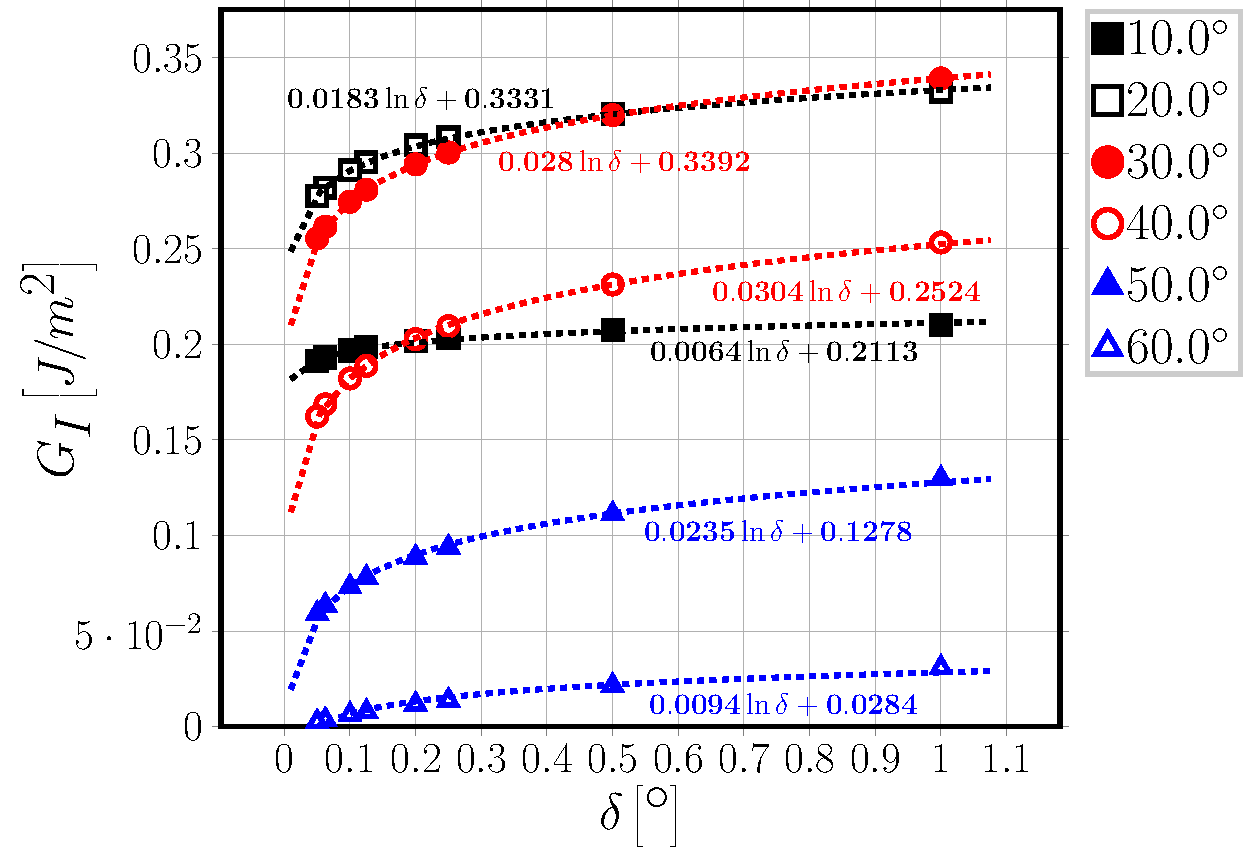
\includegraphics[width=\textwidth]{paperA/Vf0_1-free-1st-vsDelta-GI.pdf}
       \caption{$1^{st}$ order elements.}
    \end{subfigure}
    ~
    \begin{subfigure}[b]{0.48\textwidth}
        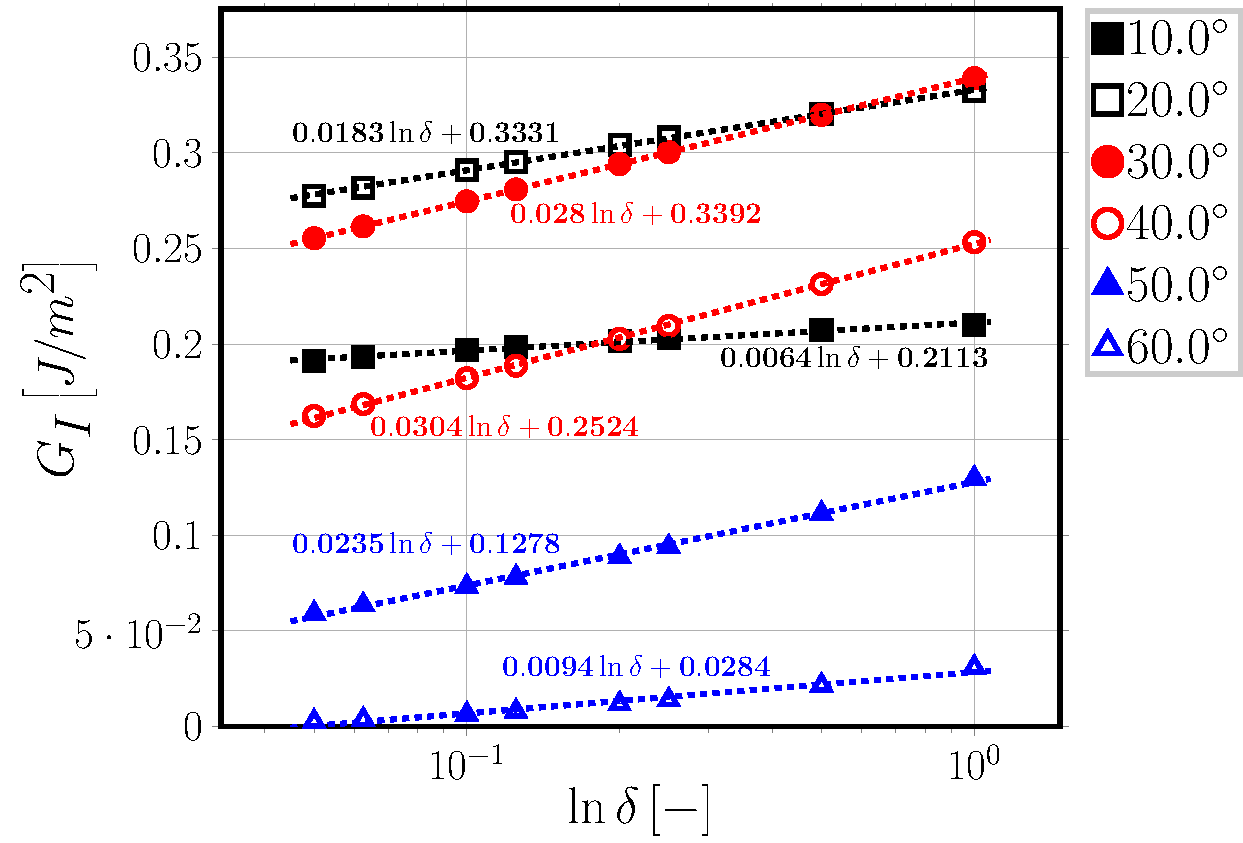
\includegraphics[width=\textwidth]{paperA/Vf0_1-free-1st-semilogvsDelta-GI.pdf}
       \caption{$1^{st}$ order elements.}
    \end{subfigure}

    \begin{subfigure}[b]{0.48\textwidth}
        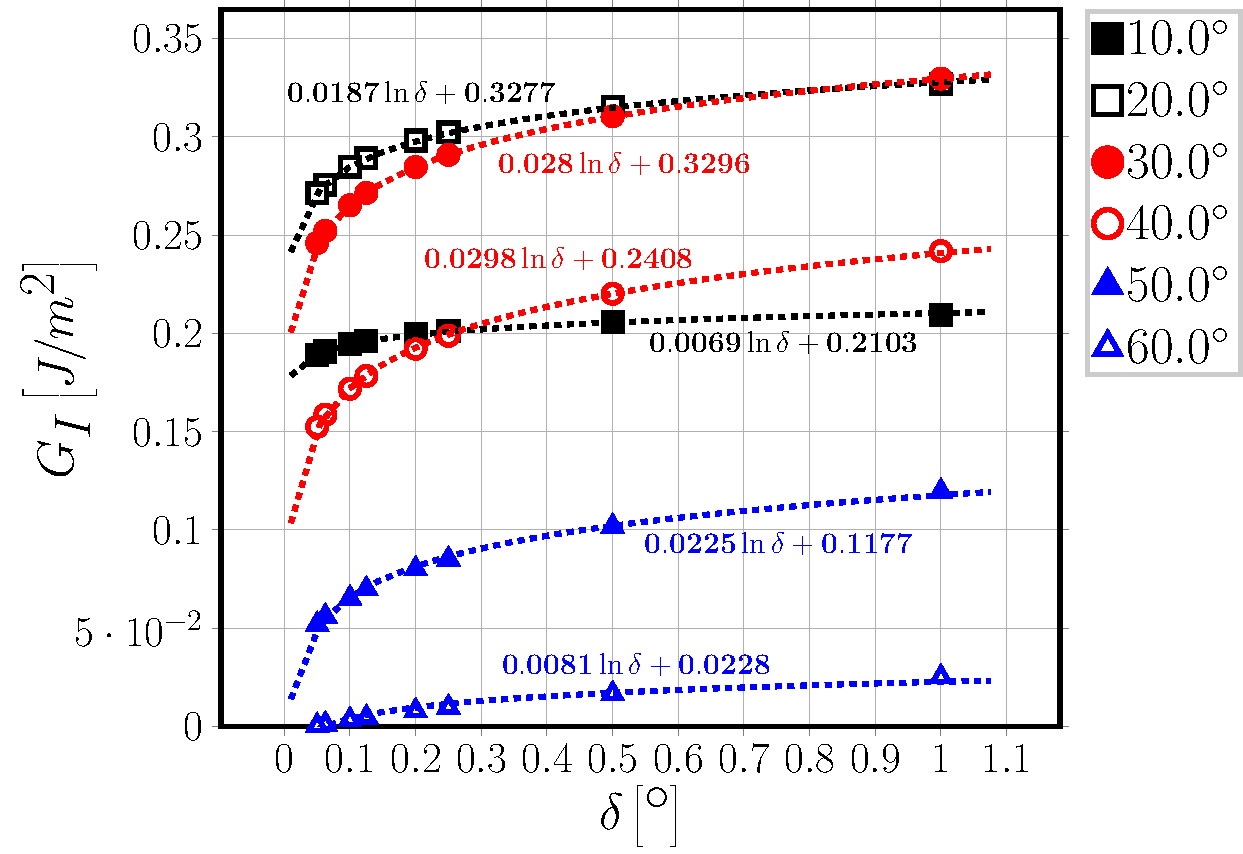
\includegraphics[width=\textwidth]{paperA/Vf0_1-free-2nd-vsDelta-GI.pdf}
       \caption{$2^{nd}$ order elements.}
    \end{subfigure}
    ~
    \begin{subfigure}[b]{0.48\textwidth}
        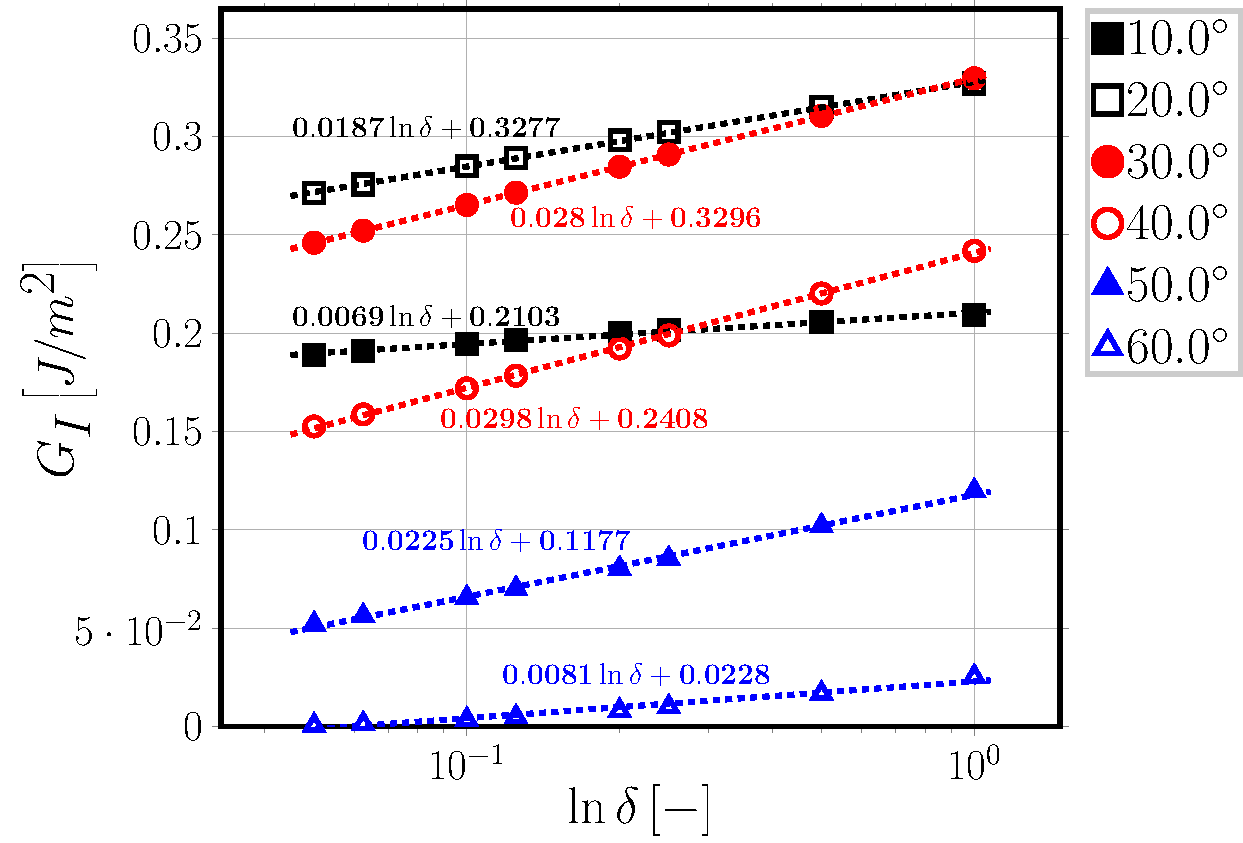
\includegraphics[width=\textwidth]{paperA/Vf0_1-free-2nd-semilogvsDelta-GI.pdf}
       \caption{$2^{nd}$ order elements.}
    \end{subfigure}

\caption{Logarithmic dependence on $\delta$ of Mode I ERR: interpolation of numerical results for $V_{f}=0.1\%$.}\label{paperA:fig:giinterp01}
\end{figure}

\begin{figure}[!h]
\centering
    \begin{subfigure}[b]{0.48\textwidth}
        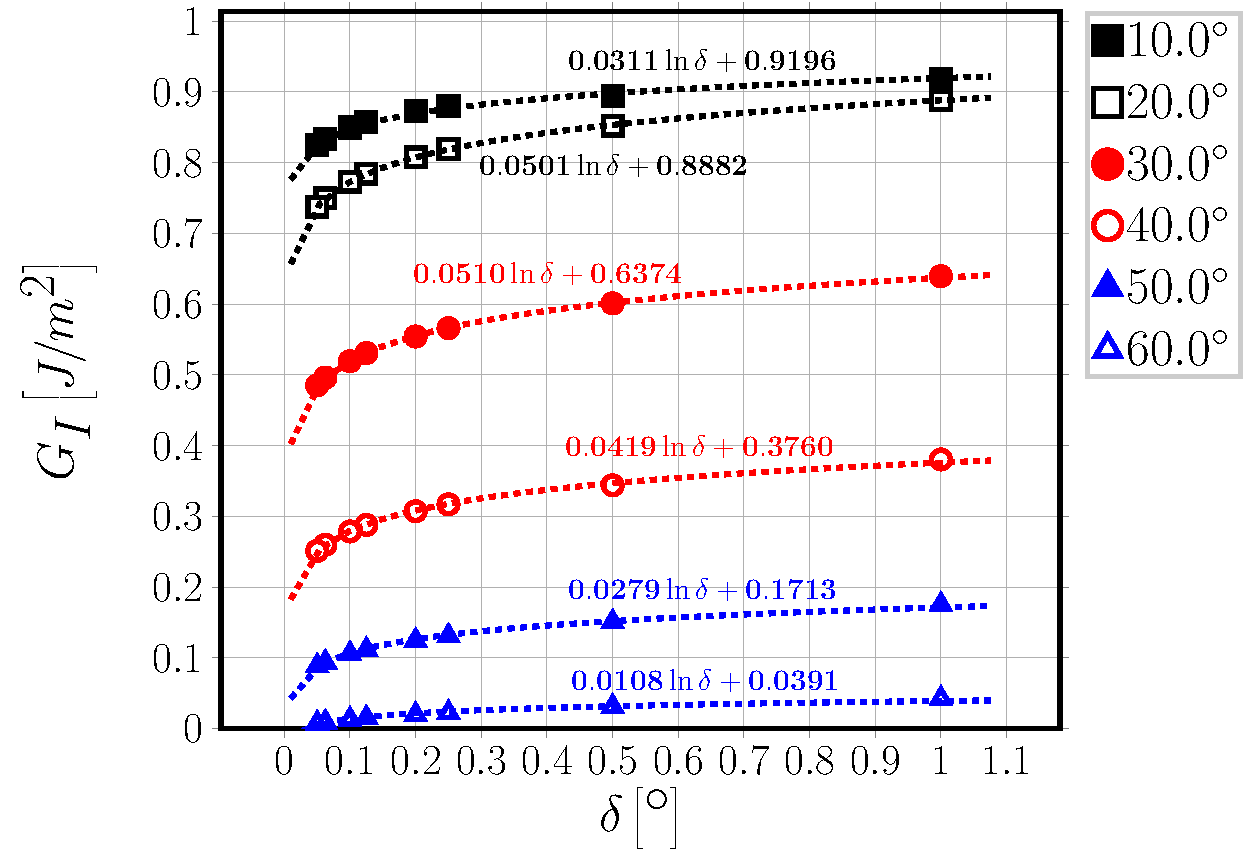
\includegraphics[width=\textwidth]{paperA/Vf40-free-1st-vsDelta-GI.pdf}
       \caption{$1^{st}$ order elements.}
    \end{subfigure}
    ~
    \begin{subfigure}[b]{0.48\textwidth}
        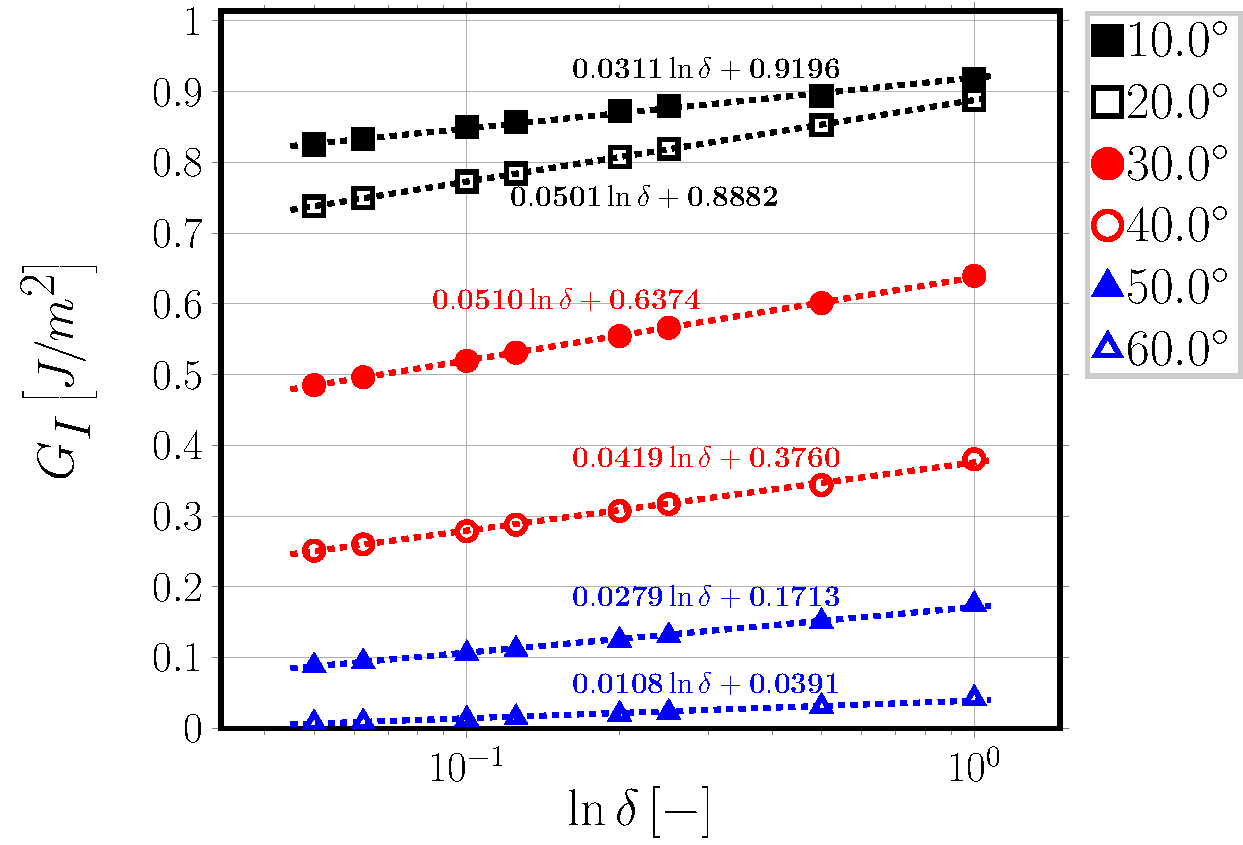
\includegraphics[width=\textwidth]{paperA/Vf40-free-1st-semilogvsDelta-GI.pdf}
       \caption{$1^{st}$ order elements.}
    \end{subfigure}

    \begin{subfigure}[b]{0.48\textwidth}
        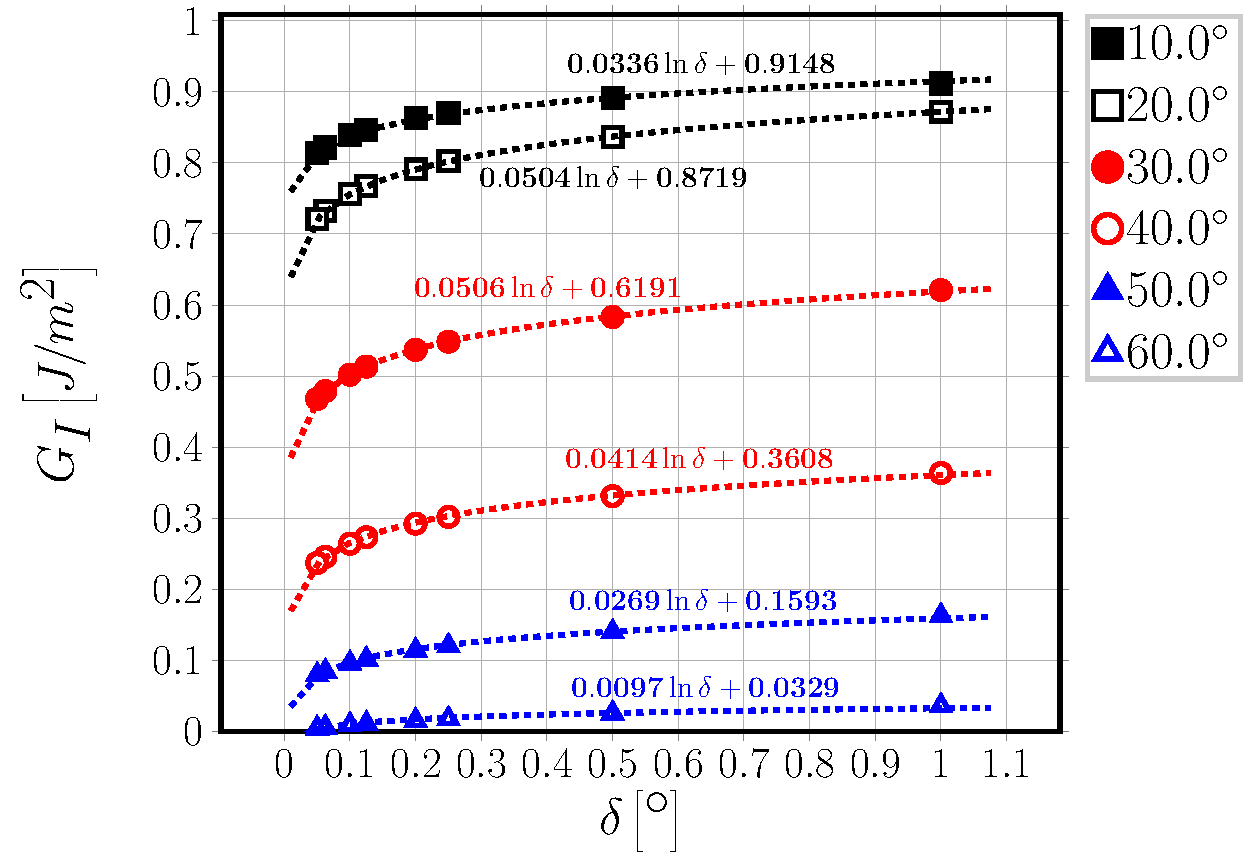
\includegraphics[width=\textwidth]{paperA/Vf40-free-2nd-vsDelta-GI.pdf}
       \caption{$2^{nd}$ order elements.}
    \end{subfigure}
    ~
    \begin{subfigure}[b]{0.48\textwidth}
        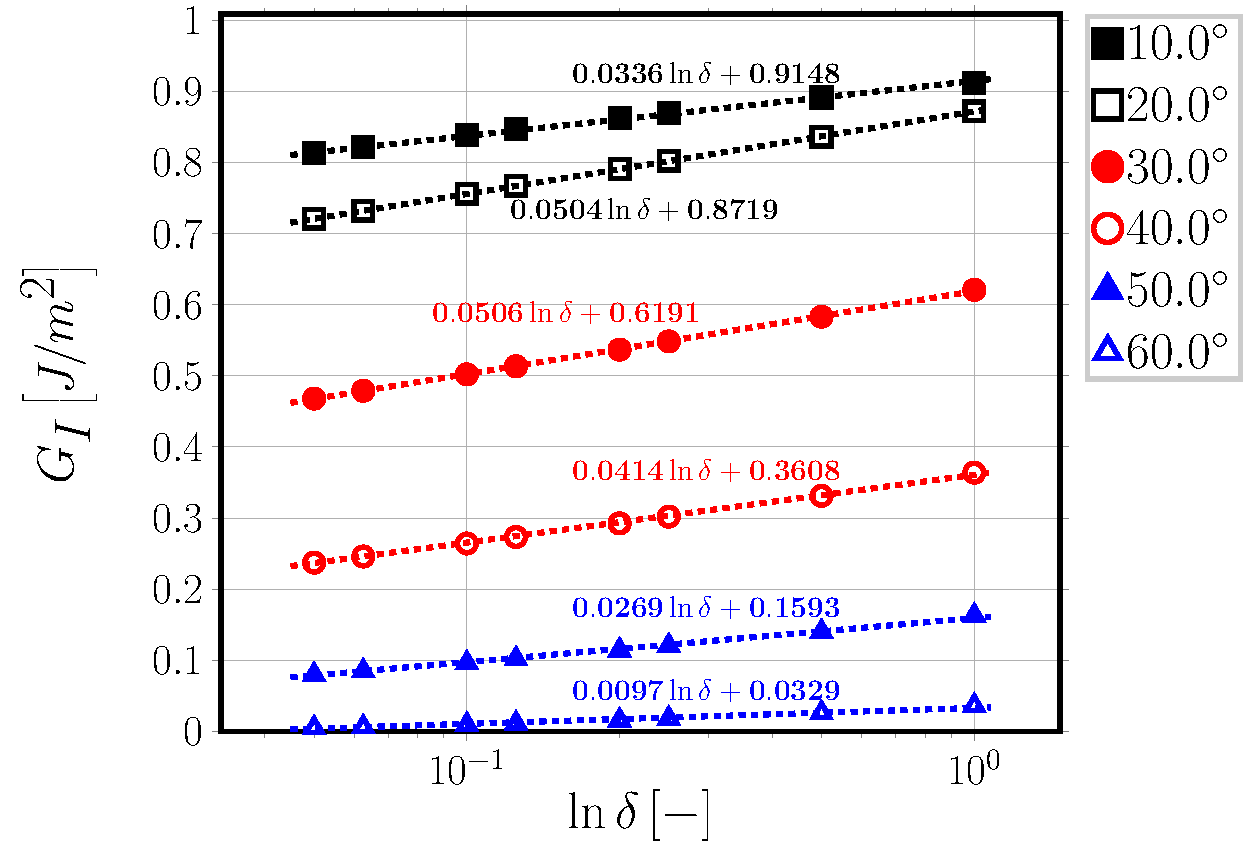
\includegraphics[width=\textwidth]{paperA/Vf40-free-2nd-semilogvsDelta-GI.pdf}
       \caption{$2^{nd}$ order elements.}
    \end{subfigure}

\caption{Logarithmic dependence on $\delta$ of Mode I ERR: interpolation of numerical results for $V_{f}=40\%$.}\label{paperA:fig:giinterp40}
\end{figure}

\begin{figure}[!h]
\centering
    \begin{subfigure}[b]{0.48\textwidth}
        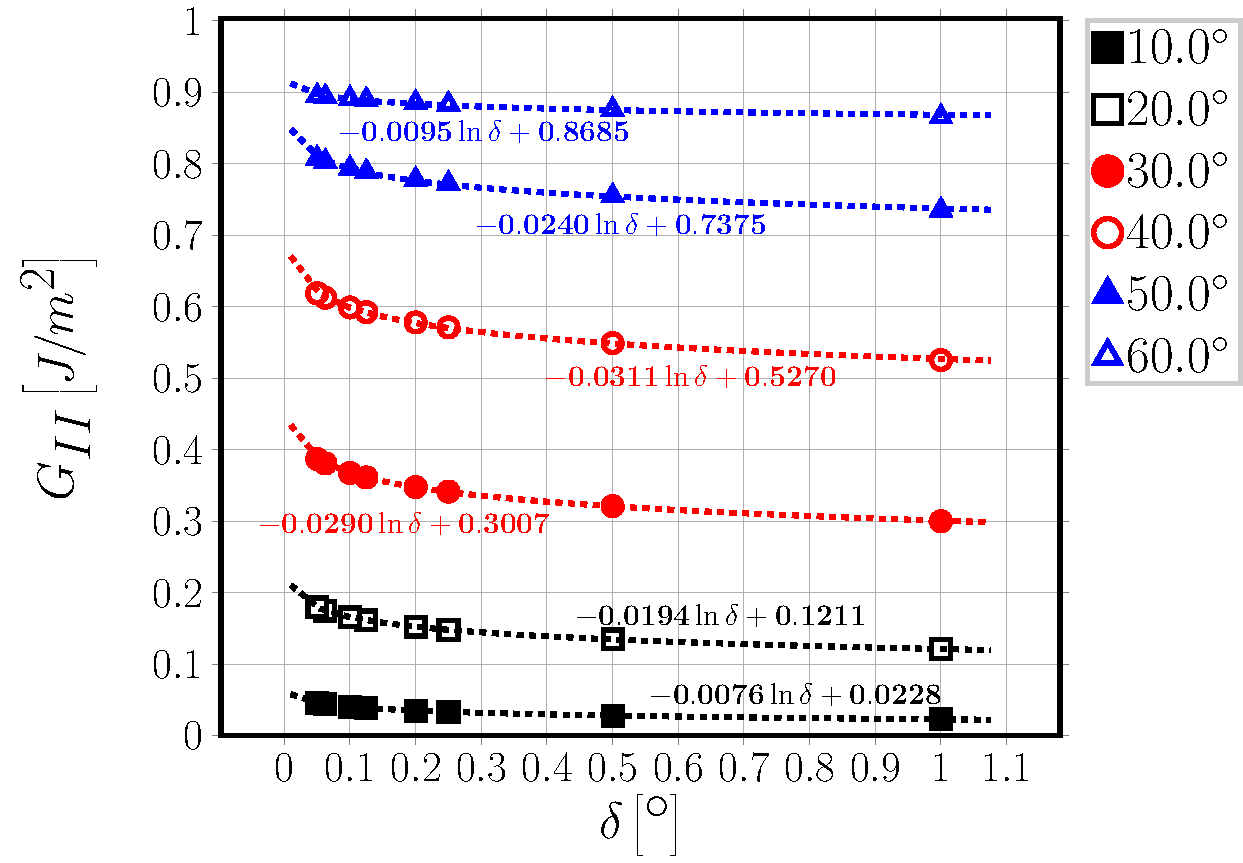
\includegraphics[width=\textwidth]{paperA/Vf0_1-free-1st-vsDelta-GII.pdf}
       \caption{$1^{st}$ order elements.}
    \end{subfigure}
    ~
    \begin{subfigure}[b]{0.48\textwidth}
        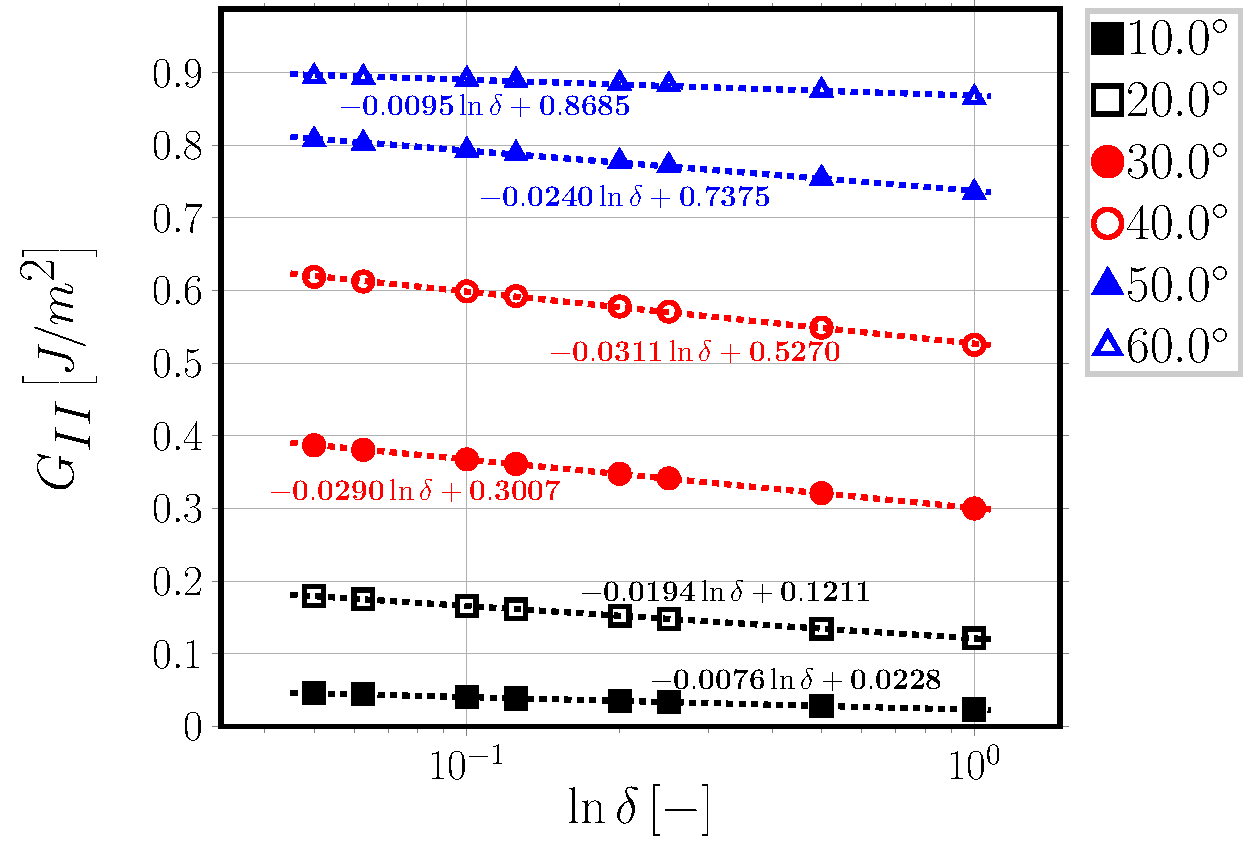
\includegraphics[width=\textwidth]{paperA/Vf0_1-free-1st-semilogvsDelta-GII.pdf}
       \caption{$1^{st}$ order elements.}
    \end{subfigure}

    \begin{subfigure}[b]{0.48\textwidth}
        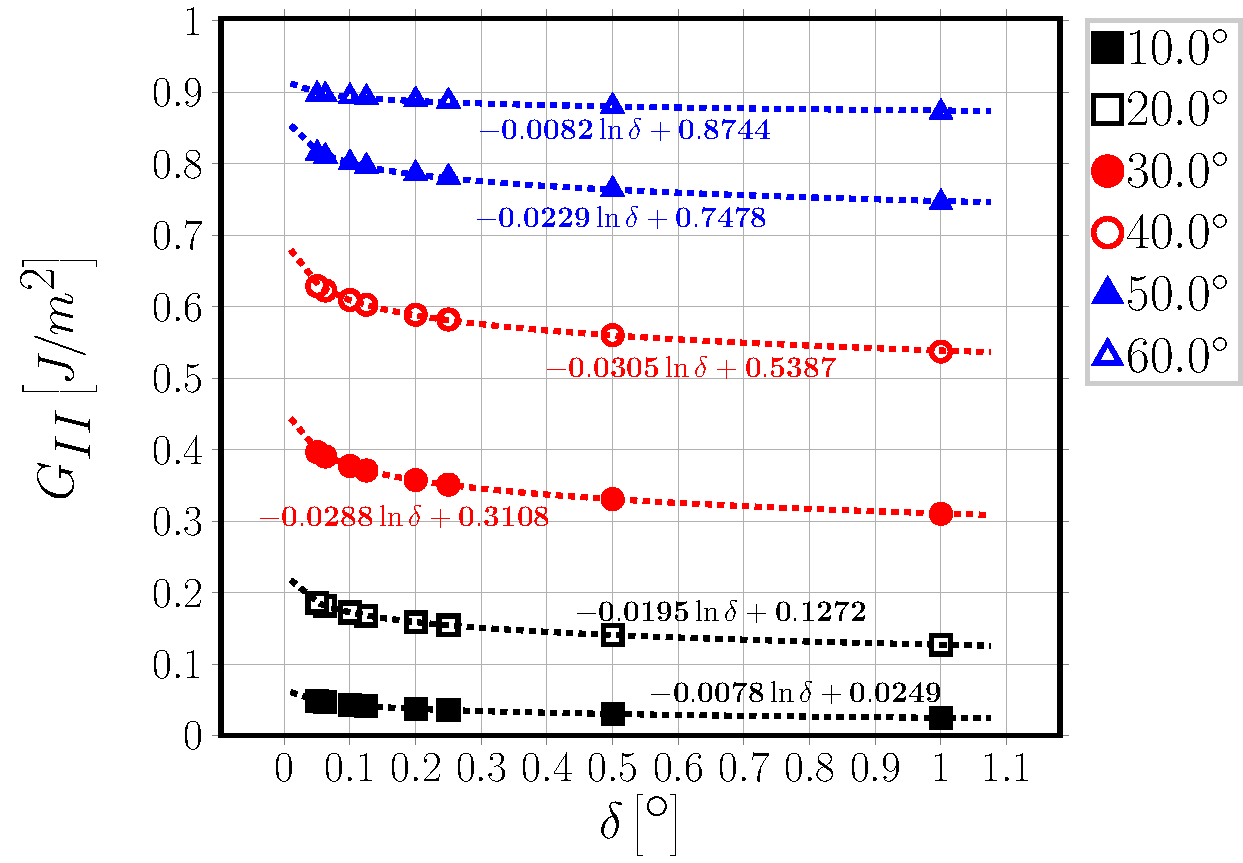
\includegraphics[width=\textwidth]{paperA/Vf0_1-free-2nd-vsDelta-GII.pdf}
       \caption{$2^{nd}$ order elements.}
    \end{subfigure}
    ~
    \begin{subfigure}[b]{0.48\textwidth}
        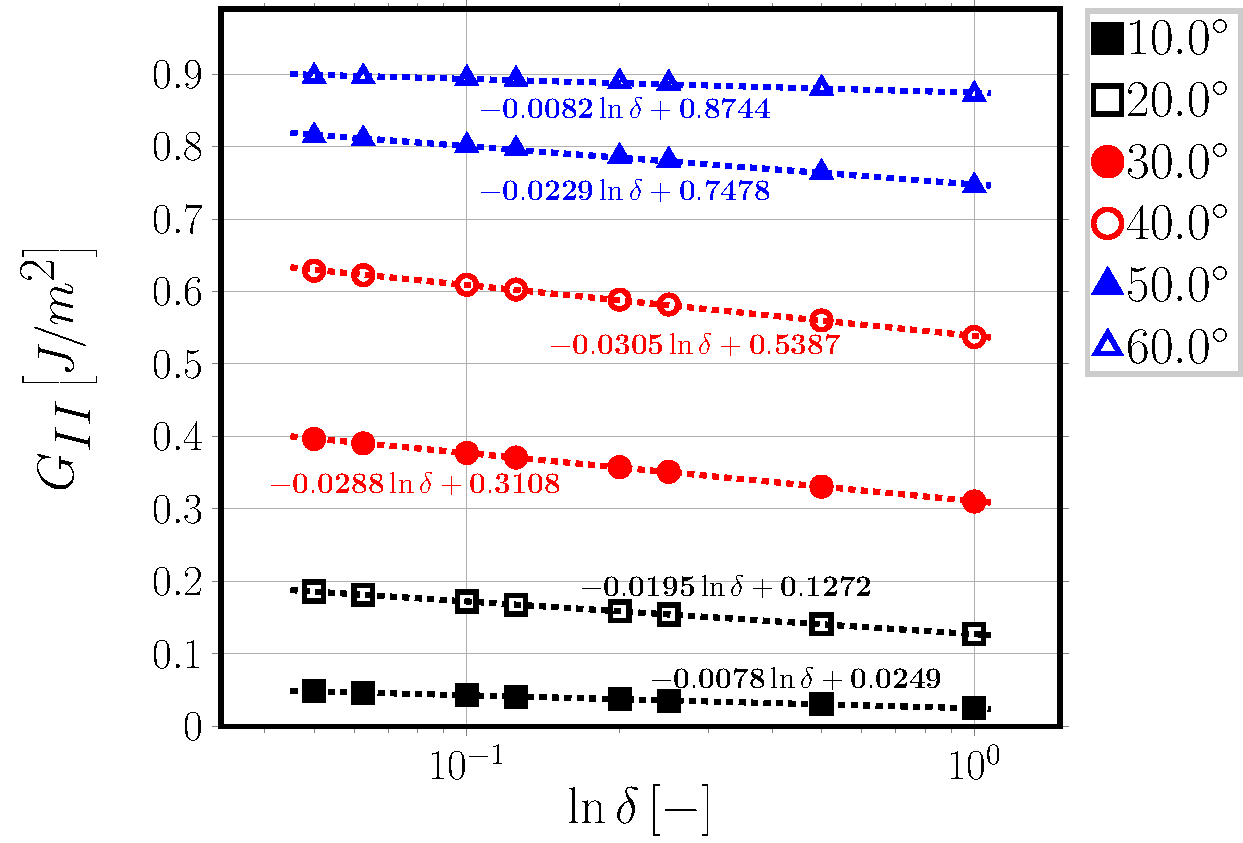
\includegraphics[width=\textwidth]{paperA/Vf0_1-free-2nd-semilogvsDelta-GII.pdf}
       \caption{$2^{nd}$ order elements.}
    \end{subfigure}

\caption{Logarithmic dependence on $\delta$ of Mode II ERR: interpolation of numerical results for $V_{f}=0.1\%$.}\label{paperA:fig:giiinterp01}
\end{figure}

\begin{figure}[!h]
\centering
    \begin{subfigure}[b]{0.48\textwidth}
        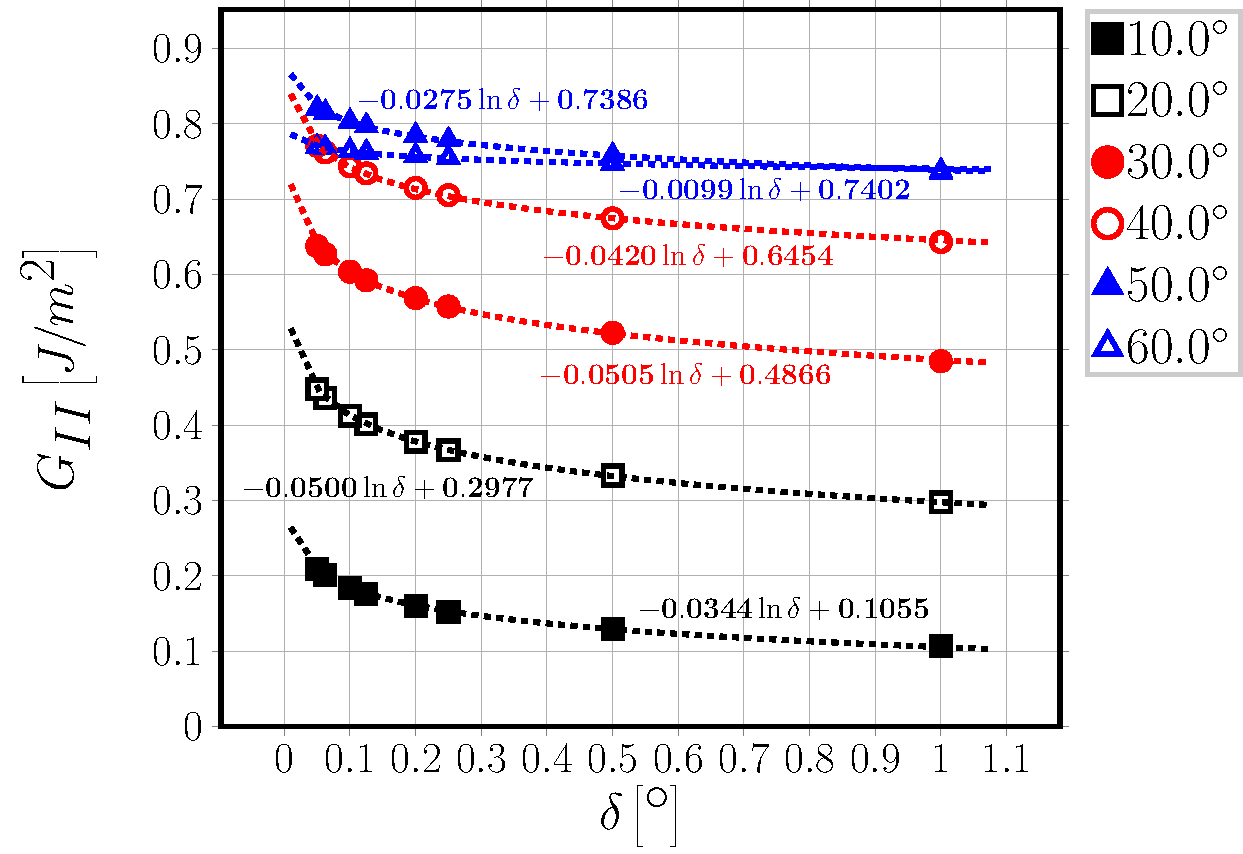
\includegraphics[width=\textwidth]{paperA/Vf40-free-1st-vsDelta-GII.pdf}
       \caption{$1^{st}$ order elements.}
    \end{subfigure}
    ~
    \begin{subfigure}[b]{0.48\textwidth}
        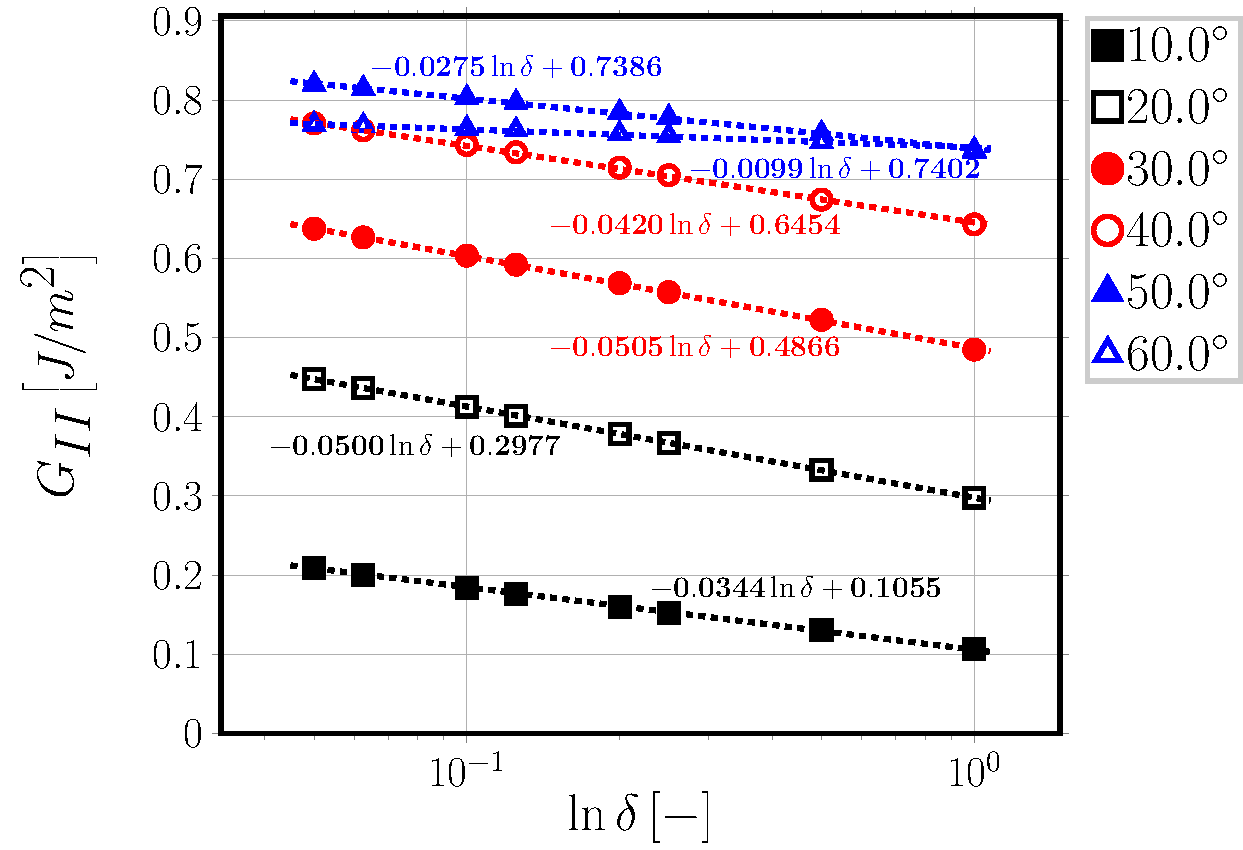
\includegraphics[width=\textwidth]{paperA/Vf40-free-1st-semilogvsDelta-GII.pdf}
       \caption{$1^{st}$ order elements.}
    \end{subfigure}

    \begin{subfigure}[b]{0.48\textwidth}
        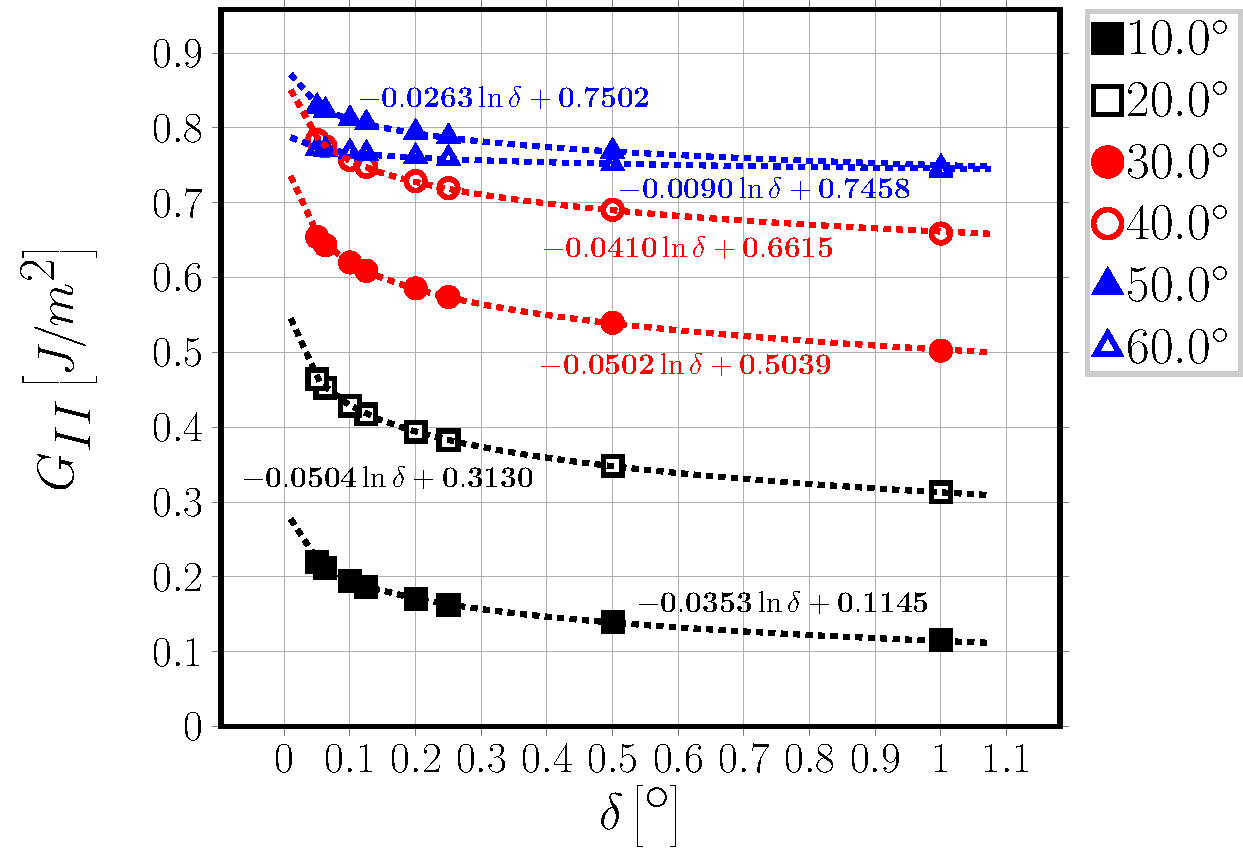
\includegraphics[width=\textwidth]{paperA/Vf40-free-2nd-vsDelta-GII.pdf}
       \caption{$2^{nd}$ order elements.}
    \end{subfigure}
    ~
    \begin{subfigure}[b]{0.48\textwidth}
        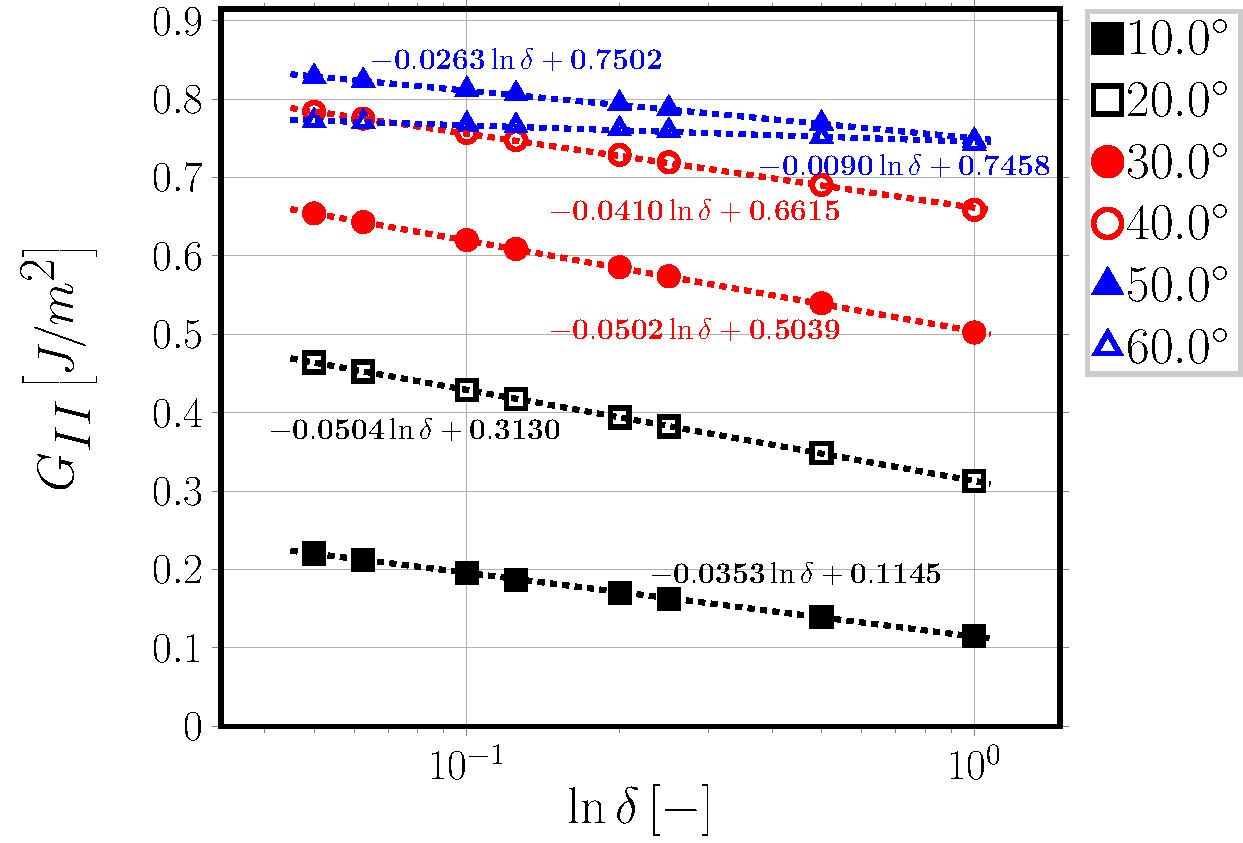
\includegraphics[width=\textwidth]{paperA/Vf40-free-2nd-semilogvsDelta-GII.pdf}
       \caption{$2^{nd}$ order elements.}
    \end{subfigure}

\caption{Logarithmic dependence on $\delta$ of Mode II ERR: interpolation of numerical results for $V_{f}=40\%$.}\label{paperA:fig:giiinterp40}
\end{figure}

As shown in Fig.~\ref{paperA:fig:giinterp01}, Fig.~\ref{paperA:fig:giinterp40}, Fig.~\ref{paperA:fig:giiinterp01} and Fig.~\ref{paperA:fig:giiinterp40} both in linear and logarithmic scales of $\delta$, the result is remarkable: both the correlation coefficient $r$ and the $r^{2}$ ratio (of explained to total variance) are always greater than $0.95$ and the $p$-values of the coefficients $A$ and $B$ are at least $<1E-6$ and often $<1E-11$ (see Table~\ref{paperA:tab:GIinterp} for $G_{I}$ and Table~\ref{paperA:tab:GIIinterp} for $G_{II}$). The results of the linear regression confirm the analytical derivations of the previous section, which showed the logarithmic behavior of Mode I and Mode II ERR. Similar conclusions were reached in~\cite{Sun1987,Manoharan1990} for a straight bi-material crack with respect to the parameter $\nicefrac{\Delta a}{a}$; however, no functional expression of $G_{\left(\cdot\right)}$ was proposed.

\section{Conclusions \& Outlook}

The application of the Virtual Crack Closure Technique to the calculation of Mode I, Mode II and total Energy Release Rate was analyzed in the context of the Finite Element solution of the bi-material circular arc crack, or fiber-matrix interface crack. A synthetic vectorial formulation of the VCCT has been proposed and its usefulness exemplified in the analysis of the mesh dependency. By both analytical considerations and numerical simulations, it has been shown that:

\begin{itemize}
\item the total ERR is invariant to rotations of the reference frame (and more in general to linear transformations), which implies that rotation of crack tip forces and displacement is actually not required in the use of the VCCT for the calculation of $G_{TOT}$;
\item the total ERR does not depend on the size $\delta$ of the elements at the crack tip, at least for reasonably small elements ($\delta\leq1.0^{\circ}$) ;
\item as a consequence, Mode II ERR for the \emph{closed} interface crack does not depend on $\delta$, as $G_{II}=G_{TOT}$ after the onset of the contact zone;
\item for the \emph{open} interface crack, Mode I and Mode II ERR depend on the element size $\delta$ through a logarithmic law of the type $A\left(\Delta\theta\right)\ln\delta+B\left(\Delta\theta\right)$;
\item the sign of the logarithm is always positive for $G_{I}$, i.e. it decreases when $\delta$ decreases, and negative for $G_{II}$, i.e. it increases when $\delta$ decreases.
\end{itemize}

The conclusion is significant: as the behavior of Mode I and Mode II is logarithmic with respect to mesh size, there exists no asymptotic limit and thus no convergence of the values. A convergence analysis based on the reduction of the error between successive iterations would not provide a reliable assessment of the accuracy of the FE solution of Mode I and Mode II Energy Release Rate of the fiber-matrix interface crack. A validation is thus required with respect to data obtained through a different method, be it analytical, numerical or experimental. Moreover, it has been shown that: first, the same behavior appears when using $1^{st}$ as well as $2^{nd}$ order elements; second, no improvement is expected with the use of singular elements, as the logarithmic dependency of $G_{I}$ and $G_{II}$ is governed by the definition of ERR itself together with the asymptotic behavior of the displacement field at the crack tip. These two conclusions \replaced{put into discussion recommendations often provided by manuals of commercial FEM packages such as Abaqus~\cite{abq12}. The latter for example, in the context of VCCT-based crack propagation (Section 11.4.2 of the \emph{Abaqus Analysis User's Guide}), suggests that \textit{in most cases mesh refinement will help with obtaining a realistic result}, that \textit{results with nonlinear materials are more sensitive to meshing than results with small-strain linear elasticity} and that \textit{first-order elements generally work best for crack propagation analysis}. }{run contrary to the suggestions provided in the manuals of many commercial FEM packages, such as Abaqus~\cite{abq12} which suggests that (Section 11.4.2 of the \emph{Abaqus Analysis User's Guide}): Sharp cracks (where the crack faces lie on top of one another in the undeformed configuration) are usually modeled using small-strain assumptions. Focused meshes, [...], should normally be used for small-strain fracture mechanics evaluations. However, for a sharp crack the strain field becomes singular at the crack tip. [...] In most cases the singularity at the crack tip should be considered in small-strain analysis (when geometric nonlinearities are ignored). Including the singularity often improves the accuracy of the J-integral, the stress intensity factors, and the stress and strain calculations because the stresses and strains in the region close to the crack tip are more accurate.}. \replaced{The previous considerations might apply for cracks in isotropic mediums; however, the VCCT-based crack propagation technique is proposed in Abaqus as a suitable technique for surface-based simulation of bi-material interface debonding. We have shown that, for a circular interface crack: mesh-refinement ($h$-refinement) does not guarantee convergence of Mode I and Mode II ERR, as their dependency on element size is logarithmic; sensitivity to meshing is actually very significant in small-strain linear elasticity and depends on the nature of the linear elastic solution at the crack tip; no difference in convergence trends is observable between first and second order elements ($p$-refinement). This closing considerations are not meant to be a critique \textit{per se} to commercial software, but rather as a source of reflection on the best use of software tools. Apart from the scientific merit of the results proposed, the conclusions presented here stand as an invitation to the practitioner to avoid black-box thinking and blind application of built-in software solutions. }{We have shown that, in the context of the fiber/matrix interface crack, the convergence of the Energy Release Rate is determined by the asymptotic behavior of the elastic solution and only marginally by the choice of element order and type, thus contradicting the statements in~\cite{abq12}}.

\FloatBarrier

\section*{Acknowledgements}

Luca Di Stasio thanks Prof. Janis Varna for the useful discussions and suggestions. Luca Di Stasio gratefully acknowledges the support of the European School of Materials (EUSMAT) through the DocMASE Doctoral Programme and the European Commission through the Erasmus Mundus Programme.

%\bibliography{refs}
\section*{References}
\addcontentsline{toc}{section}{References}
\printbibliography[heading=none]

\paperappendix
\section{Derivation of the relationship between crack tip forces and displacements for first order quadrilateral elements}\label{paperA:app:ctforcesexample}

\subsection{Foundational relations}

\added{We review and present in this Section the foundational relations of the isoparametric formulation of the Finite Element Method. The objective here is to provide a theoretical foundation to the expressions in Equation~\ref{paperA:eq:ctforce1} and Equation~\ref{paperA:eq:ctforce2} and a reference for the explicit calculation of the nodal stiffness matrices proposed in Eq.~\ref{paperA:eq:ctforce1} and Eq.~\ref{paperA:eq:ctforce2}. We propose a general treatment, valid for 2- and 3-dimensional problems, so that the interested reader could evaluate the nodal stiffness matrices for both a 2- and a 3-dimensional crack. However, in order to clarify the structure of some specific objects, we explicitly write their 2-dimensional form, which is of interest for the problem of this paper.}\\
\added{Denoting by $d$ the number of geometrical dimensions of the problem ($d=2$ in the present work),} the element Jacobian $J$ and its inverse $J^{-1}$ can be expressed in general as

\begin{equation}
\added{J_{ij}=\left(e_{\xi_{j}}\right)_{i}=\frac{\partial x_{i}}{\partial\xi_{j}}
\quad
J_{ij}^{-1}=\left(e^{x_{j}}\right)_{i}=\frac{\partial \xi_{i}}{\partial x_{j}}\quad i,j=1,\dots,d}
\end{equation}

\added{where $\left(e_{\xi_{j}}\right)$ and $\left(e^{x_{j}}\right)$ are respectively the covariant and contravariant basis vectors of the mapping between global $\left\{x_{i}\right\}$ and local element $\left\{\xi_{i}\right\}$ coordinates.\\
In 2D, assuming the global coordinates are $\left\{x, y\right\}$ and the local element coordinates are $\left\{\xi, \eta\right\}$, the covariant and contravariant basis vectors assume the form}

\begin{equation}
\underline{e}_{\xi}=\begin{bmatrix}
\frac{\partial x}{\partial\xi}\\\frac{\partial y}{\partial\xi}
\end{bmatrix}\quad\underline{e}_{\eta}=\begin{bmatrix}
\frac{\partial x}{\partial\eta}\\\frac{\partial y}{\partial\eta}
\end{bmatrix},
\end{equation}

\begin{equation}
\underline{e}_{x}=\begin{bmatrix}
\frac{\partial \xi}{\partial x}\\\frac{\partial \eta}{\partial x}
\end{bmatrix}\quad\underline{e}_{y}=\begin{bmatrix}
\frac{\partial \xi}{\partial y}\\\frac{\partial \eta}{\partial y}
\end{bmatrix}.
\end{equation}

\added{and the element Jacobian $J$ and its inverse $J^{-1}$ can be computed for a 2D problem as}

\begin{equation}
\underline{\underline{J}}=\begin{bmatrix}
\underline{e}_{\xi}|\underline{e}_{\eta}
\end{bmatrix}=\begin{bmatrix}
\frac{\partial x}{\partial\xi}&\frac{\partial x}{\partial\eta}\\\frac{\partial y}{\partial\xi}&\frac{\partial y}{\partial\eta}
\end{bmatrix}\qquad\underline{\underline{J}}^{-1}=\begin{bmatrix}
\underline{e}^{x}|\underline{e}^{y}
\end{bmatrix}=\begin{bmatrix}
\frac{\partial \xi}{\partial x}&\frac{\partial \xi}{\partial y}\\\frac{\partial \eta}{\partial x}&\frac{\partial \eta}{\partial y}
\end{bmatrix}.
\end{equation}

\deleted{where $\left\{e_{\xi}, e_{\eta}\right\}$ and $\left\{e^{x}, e^{y}\right\}$ are respectively the covariant and contravariant basis vectors of the mapping between global $\left\{x, y\right\}$ and local element $\left\{\xi, \eta\right\}$ coordinates:}

Denoting \deleted{by $d$ the number of geometrical dimensions of the problem ($d=2$ in the present work) and} by $\underline{p}$ the $d\times 1$ position vector in global coordinates, we can formally introduce the $3\left(d-1\right)\times d$ matrix operator of partial differentiation $\underline{\underline{\widetilde{B}}}$ such that

\begin{equation}\label{paperA:eq:introB}
\underline{\varepsilon}\left(\underline{p}\right)=\underline{\underline{\widetilde{B}}}\cdot\underline{u}\left(\underline{p}\right),
\end{equation}

where $\underline{u}$ and $\underline{\varepsilon}$ are respectively the $d\times 1$ displacement vector and the $3\left(d-1\right)\times 1$ strain vector in Voigt notation. Denoting by $n$ the number of nodes of a generic element\replaced{, it holds that $n=s\times m$ where $s$ represents the number of sides of the element ($3$ for a triangle, $4$ for a rectangle, \dots) and $m$ the order of the shape functions ($1$ for linear shape functions, $2$ for quadratic shape functions, \dots).}{($n=s\times m$ where $s$ represents the number of sides of the element and $m$ the order of the shape functions),} \replaced{We can now }{We can furthermore} introduce the $d\times d\cdot n$ matrix \underline{\underline{N}} of shape functions such that

\begin{equation}\label{paperA:eq:introN}
\underline{u}=\underline{\underline{N}}\cdot\underline{u}_{N},
\end{equation}

where $\underline{u}_{N}$ is the $d\cdot n\times 1$ vector of element nodal variables. Having introduced $\underline{\underline{\widetilde{B}}}$ and $\underline{\underline{N}}$ in Equations~\ref{paperA:eq:introB} and~\ref{paperA:eq:introN} respectively, it is possible to define the $3\left(d-1\right)\times d\cdot n$ matrix $\underline{\underline{B}}$ of derivatives (with respect to global coordinates) of shape functions as

\begin{equation}
\underline{\underline{B}}=\underline{\underline{\widetilde{B}}}\cdot\underline{\underline{N}}.
\end{equation}

We introduce the linear elastic material behavior in the form of the $3\left(d-1\right)\times 3\left(d-1\right)$ rigidity matrix $\underline{\underline{D}}$ such that

\begin{equation}
\underline{\sigma}=\underline{\underline{D}}\cdot\underline{\varepsilon},
\end{equation}

where $\underline{\sigma}$ the $3\left(d-1\right)\times 1$ stress vector in Voigt notation. It is finally possible to define the $n\times n$ element stiffness matrix $\underline{\underline{k_{e}}}$ as

\begin{equation}\label{paperA:eq:elestiff}
\added{\underline{\underline{k_{e}}}=\int_{V_{e}\left(x_{i}\right)}\left(\underline{\underline{B}}^{T}\underline{\underline{D}}\cdot\underline{\underline{B}}\right)dV_{e}\left(x_{i}\right)=\int_{V_{e}\left(\xi_{i}\right)}\left(\underline{\underline{B}}^{T}\underline{\underline{D}}\cdot\underline{\underline{B}}\right)\sqrt{g}dV_{e}\left(\xi_{i}\right)},
\end{equation}

where $g=det\left(\underline{\underline{J}}^{T}\underline{\underline{J}}\right)$ and $V_{e}$ is the element volume. Given that isoparametric elements are always defined between $-1$ and $1$ in each dimension, Equation~\ref{paperA:eq:elestiff} can simplified to

\begin{equation}
\added{\underline{\underline{k_{e}}}=\int_{-1}^{1}\dots\int_{-1}^{1}\left(\underline{\underline{B}}^{T}\underline{\underline{D}}\cdot\underline{\underline{B}}\right)\sqrt{g}d\xi_{i}},
\end{equation}

which is amenable to numerical integration by means of a Gaussian quadrature of the form

\begin{equation}\label{paperA:eq:elstiffnum}
\underline{\underline{k_{e}}}\approx \underbrace{\sum_{k=1}^{N}\dots\sum_{h=1}^{N}}_{d\ times}w_{k}\dots w_{h}\left(\underline{\underline{B}}^{T}\left(\xi_{i}\left(k, \dots,h\right)\right)\cdot\underline{\underline{D}}\cdot\underline{\underline{B}}\left(\xi_{i}\left(k, \dots,h\right)\right)\sqrt{g}\right),
\end{equation}

where \replaced{$\xi_{i}\left(k, \dots,h\right)$ }{$\left(\xi_{i}, \dots,\eta_{j}\right)$} are the coordinates of the $N$ Gaussian quadrature points. \replaced{The element stiffness matrix as evaluated in Eq.~\ref{paperA:eq:elstiffnum} is in general a full symmetric matrix in the case of linear elasticity. For 2D rectangular elements with quadratic shape functions (8-nodes serendipity elements), the element stiffness matrix has the form }{The element stiffness matrix as evaluated in Eq.~\ref{paperA:eq:elstiffnum} is in general a full symmetric (in the case of linear elasticity) matrix of the form}

\begin{equation}\label{paperA:eq:elstiffmatrix}
k_{e}=\begin{bmatrix}
k_{e|11}&k_{e|12}&k_{e|13}&k_{e|14}&k_{e|15}&k_{e|16}&k_{e|17}&k_{e|18}\\
k_{e|12}&k_{e|22}&k_{e|23}&k_{e|24}&k_{e|25}&k_{e|26}&k_{e|27}&k_{e|28}\\
k_{e|13}&k_{e|23}&k_{e|33}&k_{e|34}&k_{e|35}&k_{e|36}&k_{e|37}&k_{e|38}\\
k_{e|14}&k_{e|24}&k_{e|34}&k_{e|44}&k_{e|45}&k_{e|46}&k_{e|47}&k_{e|48}\\
k_{e|15}&k_{e|25}&k_{e|35}&k_{e|45}&k_{e|55}&k_{e|56}&k_{e|57}&k_{e|58}\\
k_{e|16}&k_{e|26}&k_{e|36}&k_{e|46}&k_{e|56}&k_{e|66}&k_{e|67}&k_{e|68}\\
k_{e|17}&k_{e|27}&k_{e|37}&k_{e|47}&k_{e|57}&k_{e|67}&k_{e|77}&k_{e|78}\\
k_{e|18}&k_{e|28}&k_{e|38}&k_{e|48}&k_{e|58}&k_{e|68}&k_{e|78}&k_{e|88}\\
\end{bmatrix}.
\end{equation}

\subsection{Calculation of displacements and reaction forces}

With reference to Fig.~\ref{paperA:fig:vcctlinearapp}, we define:

\begin{description}
\item[$u_{x,M}$, $u_{x,F}$] the $x$-displacement of the nodes belonging to the free side of the first element belonging to the crack, respectively on the matrix (bulk) and fiber (inclusion) side;
\item[$u_{y,M}$, $u_{y,F}$] the $y$-displacement of the nodes belonging to the free side of the first element belonging to the crack, respectively on the matrix (bulk) and fiber (inclusion) side;
\item[$u_{r,M}$, $u_{r,F}$] the $r$-displacement of the nodes belonging to the free side of the first element belonging to the crack, respectively on the matrix (bulk) and fiber (inclusion) side;
\item[$u_{\theta,M}$, $u_{\theta,F}$] the $\theta$-displacement of the nodes belonging to the free side of the first element belonging to the crack, respectively on the matrix (bulk) and fiber (inclusion) side;
\item[$F_{x,CT}$, $F_{y,CT}$] respectively the $x$- and $y$-component of the reaction force at the crack tip;
\item[$F_{r,CT}$, $F_{\theta,CT}$] respectively the $r$- and $\theta$-component of the reaction force at the crack tip.
\end{description}

The $x-y$ reference frame is the global reference frame, while the $r-\theta$ reference frame is such that the $\theta$ direction coincides with the crack propagation direction at the crack tip and $r$ the in-plane normal to the propagation direction. For an arc-crack as the present one, the $r$-direction coincides with the radial direction of the inclusion.

\begin{figure}[!h]
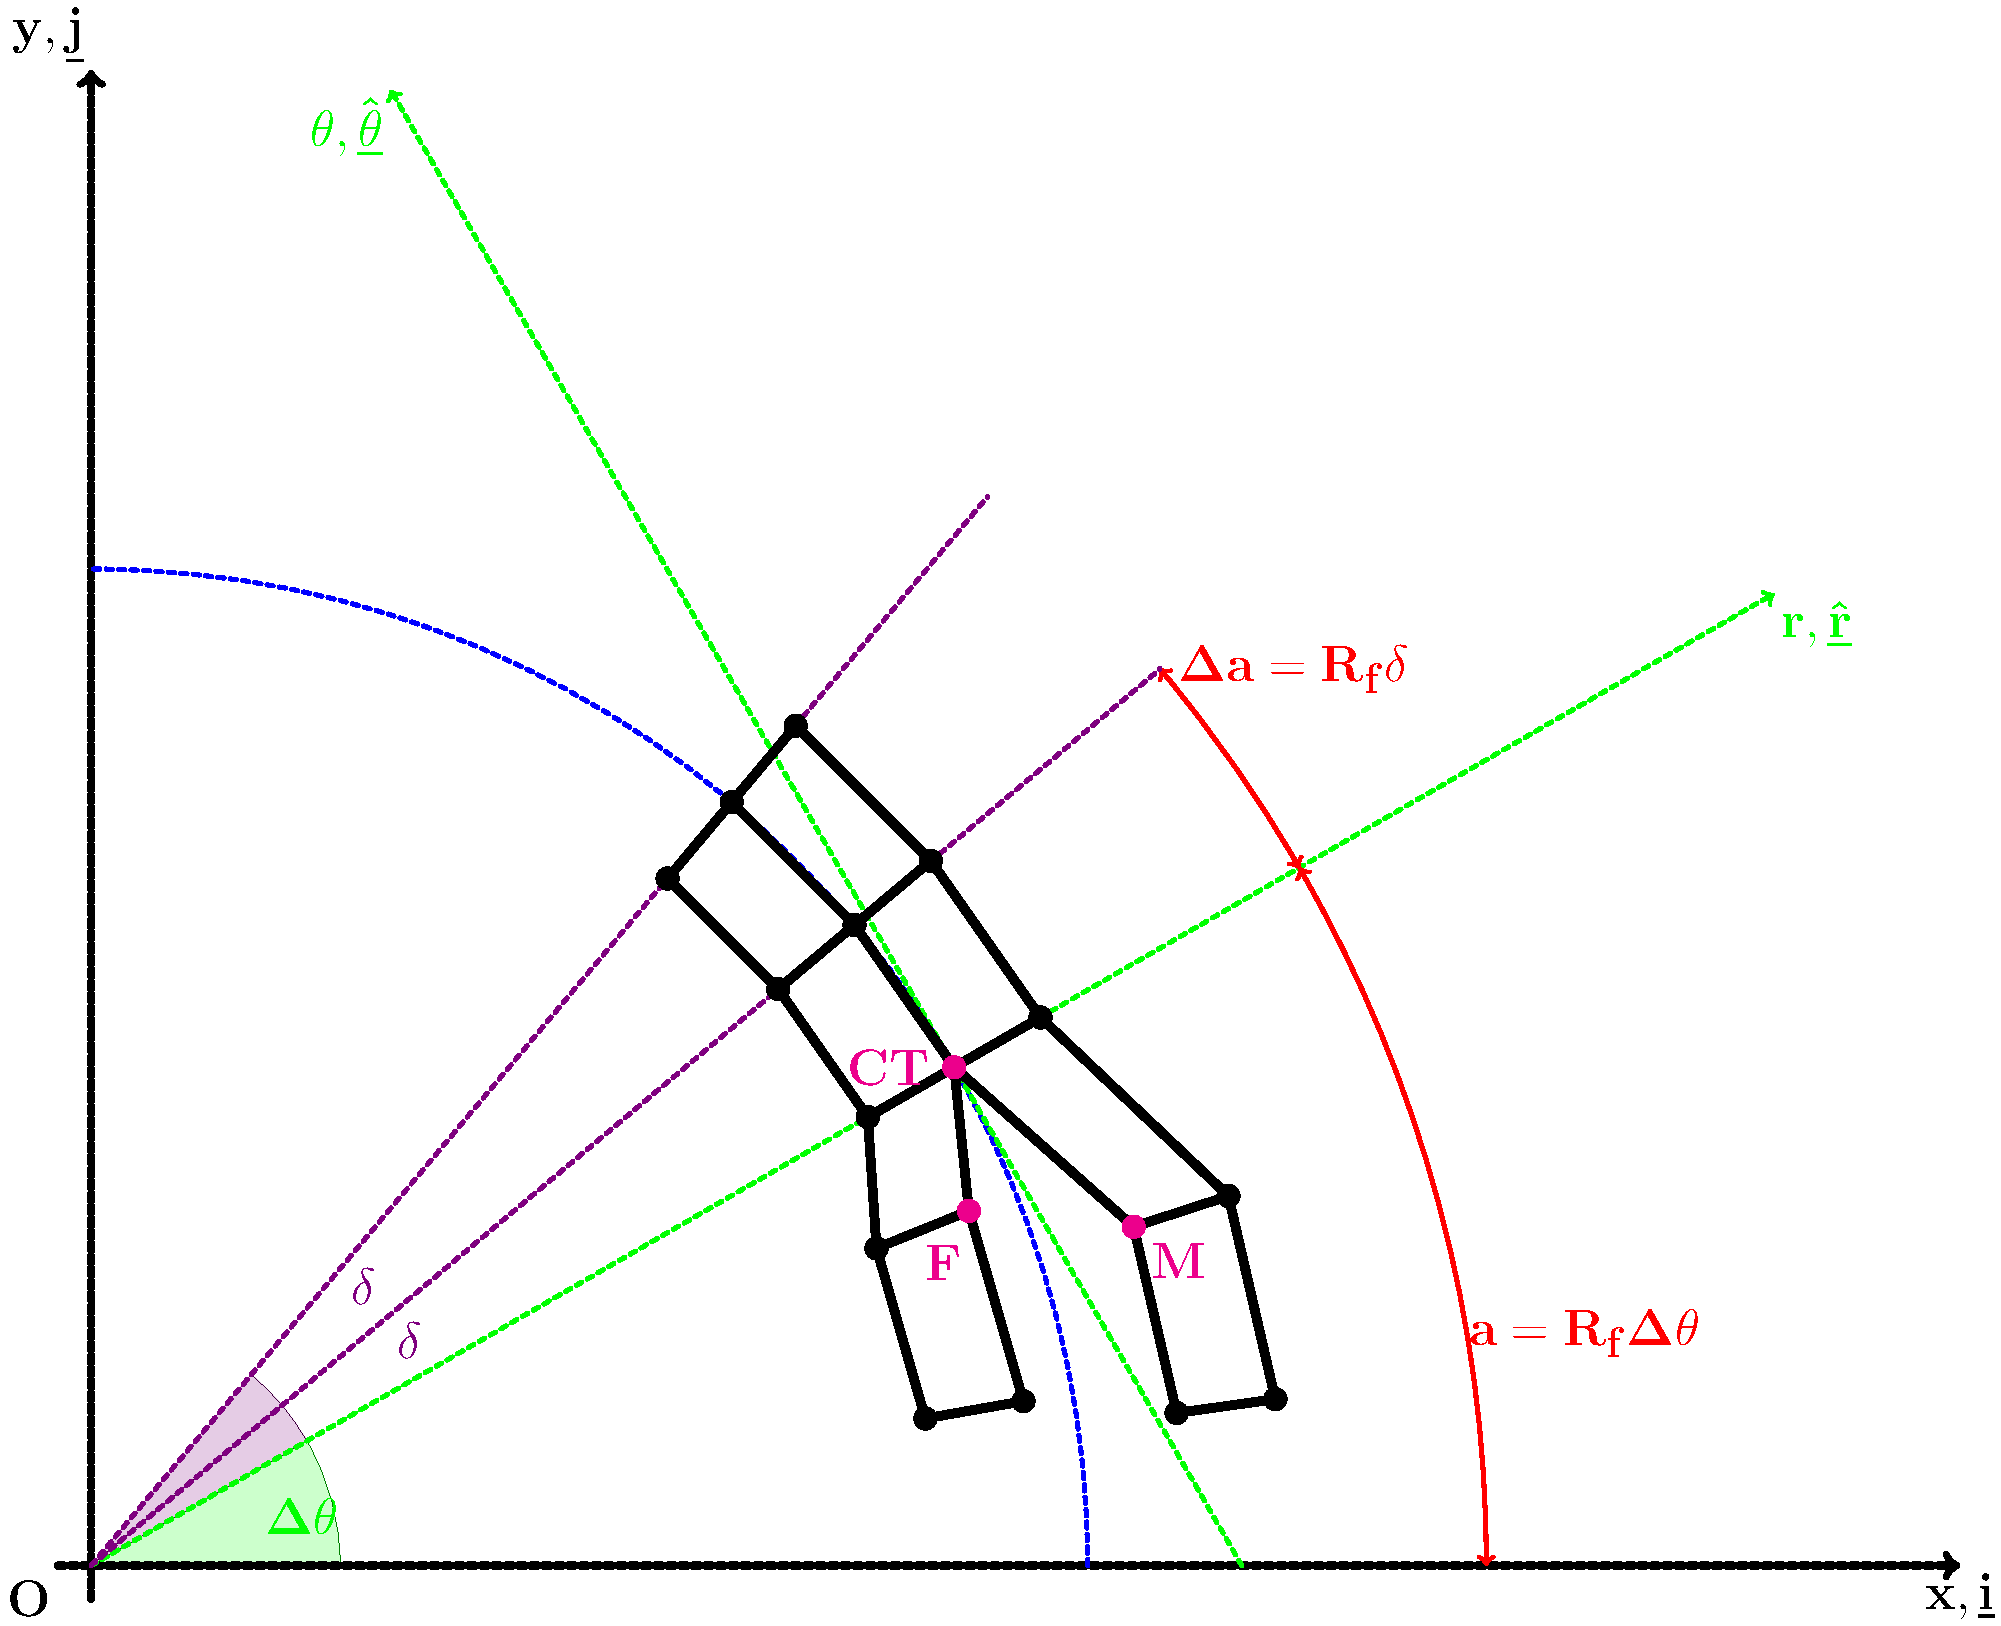
\includegraphics[width=\textwidth]{paperA/VCCT-linear-appendix.pdf}
\caption{Schematic representation of the discretized crack tip geometry for  $1^{st}$ order quadrilateral elements.}\label{paperA:fig:vcctlinearapp}
\end{figure}

The crack opening displacement $u_{r}$ and the crack shear displacement $u_{\theta}$ at the crack tip can thus be written as

\begin{equation}
u_{r}=\cos\left(\Delta\theta\right) u_{x}+\sin\left(\Delta\theta\right) u_{y}\qquad u_{\theta}=-\sin\left(\Delta\theta\right) u_{x}+\cos\left(\Delta\theta\right) u_{y},
\end{equation}

where $u_{x}$ and $u_{y}$ are defined as

\begin{equation}\label{paperA:eq:uxuy}
u_{x}=u_{x,M}-u_{x,F}\qquad u_{y}=u_{y,M}-u_{y,F}
\end{equation}

and $2\Delta\theta$ is total angular size of the debond. The corresponding forces at the crack tip are

\begin{equation}
F_{r}=\cos\left(\Delta\theta\right) F_{x,CT}+\sin\left(\Delta\theta\right) F_{y,CT}\qquad F_{\theta}=-\sin\left(\Delta\theta\right) F_{x,CT}+\cos\left(\Delta\theta\right) F_{y,CT}.
\end{equation}

At the crack tip, the FE mesh possesses two coincident points, labeled $FCT$ and $MCT$. Continuity of the displacements at the crack tip must be ensured. Furthermore, in order to measure the force at the crack tip, a fully-constraint dummy node needs to be created and formally linked to the two nodes at the crack tip by the conditions

\begin{equation}
\begin{cases}
&u_{x,FCT}-u_{x,MCT}-u_{x,DUMMY}=0\\
&u_{y,FCT}-u_{y,MCT}-u_{y,DUMMY}=0\\[10pt]
&u_{x,DUMMY}=0\\
&u_{y,DUMMY}=0\\
\end{cases},
\end{equation}

which can be simplified to

\begin{equation}
\begin{cases}
&u_{x,FCT}=u_{x,MCT}\\
&u_{y,FCT}=u_{y,MCT}\\[10pt]
&R_{x,DUMMY}=R_{x,FCT}=-R_{x,MCT}=F_{x,CT}\\
&R_{y,DUMMY}=R_{y,FCT}=-R_{y,MCT}=F_{y,CT}\\
\end{cases}.
\end{equation}

Making use of Eq.~\ref{paperA:eq:elstiffmatrix}, four equations can be written in the four displacement $u_{x,FCT}$, $u_{x,MCT}$, $u_{y,FCT}$ and $u_{y,MCT}$:

\begin{equation}\label{paperA:eq:syseqs01}
\begin{cases}
&\left(k_{e,M|11}+k_{e,M|33}\right)u_{x,MCT}+\left(k_{e,M|12}+k_{e,M|34}\right)u_{y,MCT}+\\&+k_{e,M|13}u_{x,M}+k_{e,M|14}u_{y,M}+\left(k_{M|17}+k_{M|35}\right)u_{N,MC|7}+\left(k_{M|18}+k_{M|36}\right)u_{N,MC|8}+\\&+\sum_{i=5}^{6}k_{M|1i}u_{N,MC|i}+\sum_{i=7}^{8}k_{M|3i}u_{N,MB|i}+k_{M|31}u_{x,NCOI}+k_{M|32}u_{y,NCOI}=0\\[10pt]
&\left(k_{e,M|21}+k_{e,M|43}\right)u_{x,MCT}+\left(k_{e,M|22}+k_{e,M|44}\right)u_{y,MCT}+\\&+k_{e,M|23}u_{x,M}+k_{e,M|24}u_{y,M}+\left(k_{M|27}+k_{M|45}\right)u_{N,MC|7}+\left(k_{M|28}+k_{M|46}\right)u_{N,MC|8}+\\&+\sum_{i=5}^{6}k_{M|2i}u_{N,MC|i}+\sum_{i=7}^{8}k_{M|4i}u_{N,MB|i}+k_{M|41}u_{x,NCOI}+k_{M|42}u_{y,NCOI}=0\\[10pt]
&\left(k_{e,F|77}+k_{e,F|55}\right)u_{x,FCT}+\left(k_{e,F|78}+k_{e,F|56}\right)u_{y,FCT}+\\&+k_{e,F|75}u_{x,F}+k_{e,F|76}u_{y,F}+\left(k_{F|71}+k_{F|53}\right)u_{N,FC|1}+\left(k_{F|72}+k_{F|54}\right)u_{N,FC|2}+\\&+\sum_{i=2}^{3}k_{F|7i}u_{N,FC|i}+\sum_{i=1}^{2}k_{F|5i}u_{N,FB|i}+k_{F|57}u_{x,NCOI}+k_{F|58}u_{y,NCOI}=0\\[10pt]
&\left(k_{e,F|87}+k_{e,F|65}\right)u_{x,FCT}+\left(k_{e,F|88}+k_{e,F|66}\right)u_{y,FCT}+\\&+k_{e,F|85}u_{x,F}+k_{e,F|86}u_{y,F}+\left(k_{F|81}+k_{F|63}\right)u_{N,FC|1}+\left(k_{F|82}+k_{F|64}\right)u_{N,FC|2}+\\&+\sum_{i=2}^{3}k_{F|8i}u_{N,FC|i}+\sum_{i=1}^{2}k_{F|6i}u_{N,FB|i}+k_{F|67}u_{x,NCOI}+k_{F|68}u_{y,NCOI}=0\\[10pt]
\end{cases}.
\end{equation}

Solving for $u_{y,FCT}$ and $u_{y,MCT}$ the third and fourth relations in Eq.~\ref{paperA:eq:syseqs01} and substituting in the first two expressions of Eq.~\ref{paperA:eq:syseqs01}, we get

\begin{equation}\label{paperA:eq:syseqs02}
\footnotesize
\begin{cases}
&\left(k_{e,M|11}+k_{e,M|33}+k_{e,F|77}+k_{e,F|55}\right)u_{x,MCT}+\left(k_{e,M|12}+k_{e,M|34}+k_{e,F|78}+k_{e,F|56}\right)u_{y,MCT}+\\&+k_{e,M|13}u_{x,M}+k_{e,M|14}u_{y,M}+k_{e,F|75}u_{x,F}+k_{e,F|76}u_{y,F}+\\&+\left(k_{M|31}+k_{F|57}\right)u_{x,NCOI}+\left(k_{M|32}+k_{F|58}\right)u_{y,NCOI}+\\&+\left(k_{M|17}+k_{M|35}\right)u_{N,MC|7}+\left(k_{M|18}+k_{M|36}\right)u_{N,MC|8}+\left(k_{F|71}+k_{F|53}\right)u_{N,FC|1}+\left(k_{F|72}+k_{F|54}\right)u_{N,FC|2}+\\&+\sum_{i=5}^{6}k_{M|1i}u_{N,MC|i}+\sum_{i=7}^{8}k_{M|3i}u_{N,MB|i}+\sum_{i=2}^{3}k_{F|7i}u_{N,FC|i}+\sum_{i=1}^{2}k_{F|5i}u_{N,FB|i}=0\\[10pt]
&\left(k_{e,M|21}+k_{e,M|43}+k_{e,F|87}+k_{e,F|65}\right)u_{x,MCT}+\left(k_{e,M|22}+k_{e,M|44}+k_{e,F|88}+k_{e,F|66}\right)u_{y,MCT}+\\&+k_{e,M|23}u_{x,M}+k_{e,M|24}u_{y,M}+k_{e,F|85}u_{x,F}+k_{e,F|86}u_{y,F}+\\&+\left(k_{M|41}+k_{F|67}\right)u_{x,NCOI}+\left(k_{M|42}+k_{F|68}\right)u_{y,NCOI}+\\&+\left(k_{M|27}+k_{M|45}\right)u_{N,MC|7}+\left(k_{M|28}+k_{M|46}\right)u_{N,MC|8}+\left(k_{F|81}+k_{F|63}\right)u_{N,FC|1}+\left(k_{F|82}+k_{F|64}\right)u_{N,FC|2}+\\&+\sum_{i=2}^{3}k_{F|8i}u_{N,FC|i}+\sum_{i=1}^{2}k_{F|6i}u_{N,FB|i}+\sum_{i=5}^{6}k_{M|2i}u_{N,MC|i}+\sum_{i=7}^{8}k_{M|4i}u_{N,MB|i}=0\\[10pt]
\end{cases}
\end{equation}

%\begin{equation}
%\scriptsize
%\begin{cases}
%&u_{y,MCT}=-\frac{k_{e,M|11}+k_{e,M|33}+k_{e,F|77}+k_{e,F|55}}{k_{e,M|12}+k_{e,M|34}+k_{e,F|78}+k_{e,F|56}}u_{x,MCT}+\\
%&-\frac{k_{e,M|13}u_{x,M}+k_{e,M|14}u_{y,M}+k_{e,F|75}u_{x,F}+k_{e,F|76}u_{y,F}}{k_{e,M|12}+k_{e,M|34}+k_{e,F|78}+k_{e,F|56}}+\\
%&-\frac{\left(k_{M|31}+k_{F|57}\right)u_{x,NCOI}+\left(k_{M|32}+k_{F|58}\right)u_{y,NCOI}}{k_{e,M|12}+k_{e,M|34}+k_{e,F|78}+k_{e,F|56}}+\\
%&-\frac{\left(k_{M|17}+k_{M|35}\right)u_{N,MC|7}+\left(k_{M|18}+k_{M|36}\right)u_{N,MC|8}+\left(k_{F|71}+k_{F|53}\right)u_{N,FC|1}+\left(k_{F|72}+k_{F|54}\right)u_{N,FC|2}}{k_{e,M|12}+k_{e,M|34}+k_{e,F|78}+k_{e,F|56}}+\\
%&-\frac{\sum_{i=5}^{6}k_{M|1i}u_{N,MC|i}+\sum_{i=7}^{8}k_{M|3i}u_{N,MB|i}+\sum_{i=2}^{3}k_{F|7i}u_{N,FC|i}+\sum_{i=1}^{2}k_{F|5i}u_{N,FB|i}}{k_{e,M|12}+k_{e,M|34}+k_{e,F|78}+k_{e,F|56}}\\[10pt]
%
%&\left[\left(k_{e,M|21}+k_{e,M|43}+k_{e,F|87}+k_{e,F|65}\right)+\frac{k_{e,M|11}+k_{e,M|33}+k_{e,F|77}+k_{e,F|55}}{k_{e,M|12}+k_{e,M|34}+k_{e,F|78}+k_{e,F|56}}\left(k_{e,M|22}+k_{e,M|44}+k_{e,F|88}+k_{e,F|66}\right)\right]u_{x,MCT}+\\
%&+\left(k_{e,M|23}-\frac{k_{e,M|22}+k_{e,M|44}+k_{e,F|88}+k_{e,F|66}}{k_{e,M|12}+k_{e,M|34}+k_{e,F|78}+k_{e,F|56}}k_{e,M|13}\right)u_{x,M}+\\
%&+\left(k_{e,M|24}-\frac{k_{e,M|22}+k_{e,M|44}+k_{e,F|88}+k_{e,F|66}}{k_{e,M|12}+k_{e,M|34}+k_{e,F|78}+k_{e,F|56}}k_{e,M|14}\right)u_{y,M}+\\
%&+\left(k_{e,F|85}-\frac{k_{e,M|22}+k_{e,M|44}+k_{e,F|88}+k_{e,F|66}}{k_{e,M|12}+k_{e,M|34}+k_{e,F|78}+k_{e,F|56}}k_{e,M|75}\right)u_{x,F}+\\
%&+\left(k_{e,F|86}-\frac{k_{e,M|22}+k_{e,M|44}+k_{e,F|88}+k_{e,F|66}}{k_{e,M|12}+k_{e,M|34}+k_{e,F|78}+k_{e,F|56}}k_{e,M|76}\right)u_{y,F}+\\
%&+\left[\left(k_{M|41}+k_{F|67}\right)-\frac{k_{e,M|22}+k_{e,M|44}+k_{e,F|88}+k_{e,F|66}}{k_{e,M|12}+k_{e,M|34}+k_{e,F|78}+k_{e,F|56}}\left(k_{M|31}+k_{F|57}\right)\right]u_{x,NCOI}+\\
%&+\left[\left(k_{M|42}+k_{F|68}\right)-\frac{k_{e,M|22}+k_{e,M|44}+k_{e,F|88}+k_{e,F|66}}{k_{e,M|12}+k_{e,M|34}+k_{e,F|78}+k_{e,F|56}}\left(k_{M|32}+k_{F|58}\right)\right]u_{y,NCOI}+\\
%&+\left(k_{M|27}+k_{M|45}\right)u_{N,MC|7}+\left(k_{M|28}+k_{M|46}\right)u_{N,MC|8}+\left(k_{F|81}+k_{F|63}\right)u_{N,FC|1}+\left(k_{F|82}+k_{F|64}\right)u_{N,FC|2}+\\
%&-\frac{k_{e,M|22}+k_{e,M|44}+k_{e,F|88}+k_{e,F|66}}{k_{e,M|12}+k_{e,M|34}+k_{e,F|78}+k_{e,F|56}}\left[\left(k_{M|17}+k_{M|35}\right)u_{N,MC|7}+\left(k_{M|18}+k_{M|36}\right)u_{N,MC|8}\right]+\\&
%-\frac{k_{e,M|22}+k_{e,M|44}+k_{e,F|88}+k_{e,F|66}}{k_{e,M|12}+k_{e,M|34}+k_{e,F|78}+k_{e,F|56}}\left[\left(k_{F|71}+k_{F|53}\right)u_{N,FC|1}+\left(k_{F|72}+k_{F|54}\right)u_{N,FC|2}\right]\\
%&+\sum_{i=2}^{3}k_{F|8i}u_{N,FC|i}+\sum_{i=1}^{2}k_{F|6i}u_{N,FB|i}+\sum_{i=5}^{6}k_{M|2i}u_{N,MC|i}+\sum_{i=7}^{8}k_{M|4i}u_{N,MB|i}+\\
%&-\frac{\sum_{i=5}^{6}k_{M|1i}u_{N,MC|i}+\sum_{i=7}^{8}k_{M|3i}u_{N,MB|i}+\sum_{i=2}^{3}k_{F|7i}u_{N,FC|i}+\sum_{i=1}^{2}k_{F|5i}u_{N,FB|i}}{k_{e,M|12}+k_{e,M|34}+k_{e,F|78}+k_{e,F|56}}=0\\[10pt]
%
%&u_{x,FCT}=u_{x,MCT}\\
%&u_{y,FCT}=u_{y,MCT}\\[10pt]
%&R_{x,DUMMY}=R_{x,FCT}=-R_{x,MCT}=F_{x,CT}\\
%&R_{y,DUMMY}=R_{y,FCT}=-R_{y,MCT}=F_{y,CT}\\
%\end{cases}
%\end{equation}

Solving the system of two equations and observing that $u_{x,F},u_{y,F}\sim0$ for a stiffer inclusion as a fiber in a polymeric composite, we can express $u_{x,MCT}$ as a function of $u_{x}$ and $u_{y}$ (see Eq.~\ref{paperA:eq:uxuy}) as

\begin{equation}\label{paperA:eq:syseqs03}
\scriptsize
\begin{split}
%&u_{y,MCT}=-\frac{k_{e,M|11}+k_{e,M|33}+k_{e,F|77}+k_{e,F|55}}{k_{e,M|12}+k_{e,M|34}+k_{e,F|78}+k_{e,F|56}}u_{x,MCT}+\\
%&-\frac{k_{e,M|13}u_{x,M}+k_{e,M|14}u_{y,M}+k_{e,F|75}u_{x,F}+k_{e,F|76}u_{y,F}}{k_{e,M|12}+k_{e,M|34}+k_{e,F|78}+k_{e,F|56}}+\\
%&-\frac{\left(k_{M|31}+k_{F|57}\right)u_{x,NCOI}+\left(k_{M|32}+k_{F|58}\right)u_{y,NCOI}}{k_{e,M|12}+k_{e,M|34}+k_{e,F|78}+k_{e,F|56}}+\\
%&-\frac{\left(k_{M|17}+k_{M|35}\right)u_{N,MC|7}+\left(k_{M|18}+k_{M|36}\right)u_{N,MC|8}+\left(k_{F|71}+k_{F|53}\right)u_{N,FC|1}+\left(k_{F|72}+k_{F|54}\right)u_{N,FC|2}}{k_{e,M|12}+k_{e,M|34}+k_{e,F|78}+k_{e,F|56}}+\\
%&-\frac{\sum_{i=5}^{6}k_{M|1i}u_{N,MC|i}+\sum_{i=7}^{8}k_{M|3i}u_{N,MB|i}+\sum_{i=2}^{3}k_{F|7i}u_{N,FC|i}+\sum_{i=1}^{2}k_{F|5i}u_{N,FB|i}}{k_{e,M|12}+k_{e,M|34}+k_{e,F|78}+k_{e,F|56}}\\[10pt]
&\left[\left(k_{e,M|21}+k_{e,M|43}+k_{e,F|87}+k_{e,F|65}\right)+\frac{k_{e,M|11}+k_{e,M|33}+k_{e,F|77}+k_{e,F|55}}{k_{e,M|12}+k_{e,M|34}+k_{e,F|78}+k_{e,F|56}}\left(k_{e,M|22}+k_{e,M|44}+k_{e,F|88}+k_{e,F|66}\right)\right]u_{x,MCT}+\\
&+\left(k_{e,M|23}-\frac{k_{e,M|22}+k_{e,M|44}+k_{e,F|88}+k_{e,F|66}}{k_{e,M|12}+k_{e,M|34}+k_{e,F|78}+k_{e,F|56}}k_{e,M|13}\right)u_{x}+\\
&+\left(k_{e,M|24}-\frac{k_{e,M|22}+k_{e,M|44}+k_{e,F|88}+k_{e,F|66}}{k_{e,M|12}+k_{e,M|34}+k_{e,F|78}+k_{e,F|56}}k_{e,M|14}\right)u_{y}+\\
&+\left(k_{e,M|23}+k_{e,F|85}-\frac{k_{e,M|22}+k_{e,M|44}+k_{e,F|88}+k_{e,F|66}}{k_{e,M|12}+k_{e,M|34}+k_{e,F|78}+k_{e,F|56}}\left(k_{e,M|13}+k_{e,M|75}\right)\right)\cancelto{\approx 0}{u_{x,F}}+\\
&+\left(k_{e,M|24}+k_{e,F|86}-\frac{k_{e,M|22}+k_{e,M|44}+k_{e,F|88}+k_{e,F|66}}{k_{e,M|12}+k_{e,M|34}+k_{e,F|78}+k_{e,F|56}}\left(k_{e,M|14}+k_{e,M|76}\right)\right)\cancelto{\approx 0}{u_{y,F}}+\\
&+\left[\left(k_{M|41}+k_{F|67}\right)-\frac{k_{e,M|22}+k_{e,M|44}+k_{e,F|88}+k_{e,F|66}}{k_{e,M|12}+k_{e,M|34}+k_{e,F|78}+k_{e,F|56}}\left(k_{M|31}+k_{F|57}\right)\right]u_{x,NCOI}+\\
&+\left[\left(k_{M|42}+k_{F|68}\right)-\frac{k_{e,M|22}+k_{e,M|44}+k_{e,F|88}+k_{e,F|66}}{k_{e,M|12}+k_{e,M|34}+k_{e,F|78}+k_{e,F|56}}\left(k_{M|32}+k_{F|58}\right)\right]u_{y,NCOI}+\\
&+\left(k_{M|27}+k_{M|45}\right)u_{N,MC|7}+\left(k_{M|28}+k_{M|46}\right)u_{N,MC|8}+\left(k_{F|81}+k_{F|63}\right)u_{N,FC|1}+\left(k_{F|82}+k_{F|64}\right)u_{N,FC|2}+\\
&-\frac{k_{e,M|22}+k_{e,M|44}+k_{e,F|88}+k_{e,F|66}}{k_{e,M|12}+k_{e,M|34}+k_{e,F|78}+k_{e,F|56}}\left[\left(k_{M|17}+k_{M|35}\right)u_{N,MC|7}+\left(k_{M|18}+k_{M|36}\right)u_{N,MC|8}\right]+\\&
-\frac{k_{e,M|22}+k_{e,M|44}+k_{e,F|88}+k_{e,F|66}}{k_{e,M|12}+k_{e,M|34}+k_{e,F|78}+k_{e,F|56}}\left[\left(k_{F|71}+k_{F|53}\right)u_{N,FC|1}+\left(k_{F|72}+k_{F|54}\right)u_{N,FC|2}\right]\\
&+\sum_{i=2}^{3}k_{F|8i}u_{N,FC|i}+\sum_{i=1}^{2}k_{F|6i}u_{N,FB|i}+\sum_{i=5}^{6}k_{M|2i}u_{N,MC|i}+\sum_{i=7}^{8}k_{M|4i}u_{N,MB|i}+\\
&-\frac{\sum_{i=5}^{6}k_{M|1i}u_{N,MC|i}+\sum_{i=7}^{8}k_{M|3i}u_{N,MB|i}+\sum_{i=2}^{3}k_{F|7i}u_{N,FC|i}+\sum_{i=1}^{2}k_{F|5i}u_{N,FB|i}}{k_{e,M|12}+k_{e,M|34}+k_{e,F|78}+k_{e,F|56}}=0,
\end{split}
\end{equation}

while the reaction forces at the crack tip can be expressed as

\begin{equation}\label{paperA:eq:forcesreform}
\begin{cases}
F_{x,CT}&=R_{x,FCT}=\\&=\left(k_{e,F|77}+k_{e,F|55}\right)u_{x,FCT}+\left(k_{e,F|78}+k_{e,F|56}\right)u_{y,FCT}+\\
&+k_{e,F|75}\cancelto{\approx 0}{u_{x,F}}+k_{e,F|76}\cancelto{\approx 0}{u_{y,F}}+\\
&+\sum_{i=1}^{4}k_{e,F|7i}u_{N,FC|i}+\sum_{i=1,i\neq\left(5,6\right)}^{8}k_{e,F|5i}u_{N,FB|i}\\
F_{y,CT}&=R_{y,FCT}=\\&=\left(k_{e,F|87}+k_{e,F|65}\right)u_{x,FCT}+\left(k_{e,F|88}+k_{e,F|66}\right)u_{y,FCT}+\\
&+k_{e,F|85}\cancelto{\approx 0}{u_{x,F}}+k_{e,F|86}\cancelto{\approx 0}{u_{y,F}}+\\
&+\sum_{i=1}^{4}k_{e,F|8i}u_{N,FC|i}+\sum_{i=1,i\neq\left(5,6\right)}^{8}k_{e,F|6i}u_{N,FB|i}\\
\end{cases}.
\end{equation}

Substituting Eq.~\ref{paperA:eq:syseqs01} in Eq.~\ref{paperA:eq:syseqs02}, Eq.~\ref{paperA:eq:syseqs03} and Eq.~\ref{paperA:eq:forcesreform} and solving, we obtain an expression of the form

\begin{equation}
\begin{cases}
F_{x,CT}&= K_{xx}u_{x}+K_{xy}u_{y}+\\
&+\sum_{i=1}^{4}K_{FC,x|i}u_{N,FC|i}+\sum_{i=1,i\neq\left(3,4,5,6\right)}^{8}K_{FB,x|i}u_{N,FB|i}+\\
&+\sum_{i=5}^{8}K_{FC,x|i}u_{N,MC|i}+\sum_{i=7}^{8}K_{MB,x|i}u_{N,FB|i}\\
F_{y,CT}&= K_{yx}u_{x}+K_{yy}u_{y}+\\
&+\sum_{i=1}^{4}K_{FC,y|i}u_{N,FC|i}+\sum_{i=1,i\neq\left(3,4,5,6\right)}^{8}K_{FB,y|i}u_{N,FB|i}+\\
&+\sum_{i=5}^{8}K_{FC,y|i}u_{N,MC|i}+\sum_{i=7}^{8}K_{MB,y|i}u_{N,FB|i}\\
\end{cases},
\end{equation}

which can be reformulated synthetically as

\begin{equation}
\begin{cases}
F_{x,CT}&= K_{xx}u_{x}+K_{xy}u_{y}+\widetilde{F}_{x}\\
F_{y,CT}&= K_{yx}u_{x}+K_{yy}u_{y}+\widetilde{F}_{y}\\
\end{cases},
\end{equation}

where $\widetilde{F}_{x}$ and $\widetilde{F}_{y}$ represent the influence of the FE solution through the nodes of the elements sharing the crack tip that do not belong to any of the phase interfaces, i.e. the nodes of the elements sharing the crack tip that belong to the bulk of each phase.

\section{Expression of the VCCT weights matrix for quadrilateral elements with or without singularity}\label{paperA:app:Tpq}

The expression of $\underline{\underline{T}}_{pq}$ for quadrilateral elements with or without singularity is

\begin{equation}\label{paperA:eq:Tpq}
\scriptsize
\begin{split}
\underline{\underline{T}}_{pq}&=\begin{cases}
\underline{\underline{I}}\ for\ p=q<2\\
\underline{\underline{0}}\ otherwise
\end{cases}\quad \text{for $1^{st}$ order quadrilateral elements}\\
&=\begin{cases}
\underline{\underline{I}}\ for\ p=q<3\\
\underline{\underline{0}}\ otherwise
\end{cases}\quad \text{for $2^{nd}$ order quadrilateral elements}\\
&=\begin{cases}
\underline{\underline{I}}\ for\ p=q<4\\
\underline{\underline{0}}\ otherwise
\end{cases}\quad \text{for $3^{rd}$ order quadrilateral elements}\\
&=\begin{cases}
\left(14-\frac{33\pi}{8}\right)\underline{\underline{I}}\ for\ p=1,q=1\\
\left(-52+\frac{33\pi}{2}\right)\underline{\underline{I}}\ for\ p=1,q=2\\
\left(17-\frac{21\pi}{4}\right)\underline{\underline{I}}\ for\ p=2,q=1\\
\left(-\frac{7}{2}+\frac{21\pi}{16}\right)\underline{\underline{I}}\ for\ p=2,q=2\\
\left(8-\frac{21\pi}{8}\right)\underline{\underline{I}}\ for\ p=1,q=3\\
\left(-32+\frac{21\pi}{2}\right)\underline{\underline{I}}\ for\ p=2,q=3\\
\underline{\underline{0}}\ otherwise
\end{cases}\quad \text{for $2^{nd}$ order quarter-point quadrilateral elements}\\
&=\begin{cases}
\left(-11187+\frac{7155\pi}{2}\right)\underline{\underline{I}}\ for\ p=1,q=1\\
\left(38556-\frac{24543\pi}{2}\right)\underline{\underline{I}}\ for\ p=1,q=2\\
\left(-53055+\frac{33777\pi}{2}\right)\underline{\underline{I}}\ for\ p=1,q=3\\
\left(\frac{11396}{3}-\frac{9575\pi}{8}\right)\underline{\underline{I}}\ for\ p=2,q=1\\
\left(-12936+\frac{33003\pi}{8}\right)\underline{\underline{I}}\ for\ p=2,q=2\\
\left(17988-\frac{45837\pi}{8}\right)\underline{\underline{I}}\ for\ p=2,q=3\\
\left(-\frac{8453}{3}+\frac{3595\pi}{4}\right)\underline{\underline{I}}\ for\ p=3,q=1\\
\left(9804-\frac{12411\pi}{4}\right)\underline{\underline{I}}\ for\ p=3,q=2\\
\left(-13587+\frac{17289\pi}{4}\right)\underline{\underline{I}}\ for\ p=3,q=3\\
\left(6948-\frac{17685\pi}{8}\right)\underline{\underline{I}}\ for\ p=1,q=4\\
\left(-23976+\frac{60993\pi}{8}\right)\underline{\underline{I}}\ for\ p=2,q=4\\
\left(33372-\frac{84807\pi}{8}\right)\underline{\underline{I}}\ for\ p=3,q=4\\
\underline{\underline{0}}\ otherwise
\end{cases}\quad \text{for $3^{rd}$ order quarter-point quadrilateral elements}\\
\end{split}
\end{equation}

where $\underline{\underline{I}}$ is the identity matrix.

%\section{Derivation of the vectorial formulation of the ERR}\label{paperA:paperA:app:errvecfor}
%
%\begin{equation}
%\begin{split}
%G_{TOT} &= \frac{1}{2R_{f}\delta}\sum_{p=1}^{m+1}\sum_{q=1}^{m+1}\underline{u}_{r\theta,p}^{T}\underline{\underline{T}}_{pq}^{T}\underline{F}_{r\theta,q}=\\
%&=\frac{1}{2R_{f}\delta}\sum_{p=1}^{m+1}\sum_{q=1}^{m+1}Tr\left(\underline{F}_{r\theta,q}\underline{u}_{r\theta,p}^{T}\underline{\underline{T}}_{pq}^{T}\right)=\\&=\frac{1}{2R_{f}\delta}\sum_{p=1}^{m+1}\sum_{q=1}^{m+1}Tr\left(\begin{bmatrix}
%t_{pq|11}F_{r,q}u_{r,p}&t_{pq|12}F_{r,q}u_{\theta,p}\\
%t_{pq|21}F_{\theta,q}u_{r,p}&t_{pq|22}F_{\theta,q}u_{\theta,p}\\
%\end{bmatrix}\right)=\\
%&=\frac{1}{2R_{f}\delta}\sum_{p=1}^{m+1}\sum_{q=1}^{m+1}Tr\left(\underline{\underline{Q}}_{\delta}\underline{\underline{R}}_{\Delta\theta}\underline{F}_{xy,q}\underline{u}_{xy,p}^{T}\underline{\underline{R}}_{\Delta\theta}^{T}\underline{\underline{P}}_{\delta}^{T}\underline{\underline{T}}_{pq}^{T}\right)
%\end{split}
%\end{equation}
%
%\begin{equation}
%\underline{G}=\begin{bmatrix}
%G_{I} \\
%G_{II}
%\end{bmatrix}=\frac{1}{2R_{f}\delta}\sum_{p=1}^{m+1}\sum_{q=1}^{m+1}Diag\left(\underline{\underline{Q}}_{\delta}\underline{\underline{R}}_{\Delta\theta}\underline{F}_{xy,q}\underline{u}_{xy,p}^{T}\underline{\underline{R}}_{\Delta\theta}^{T}\underline{\underline{P}}_{\delta}^{T}\underline{\underline{T}}_{pq}^{T}\right)
%\end{equation}
%
%\begin{equation}
%\begin{split}
%\underline{G}=\begin{bmatrix}
%G_{I} \\
%G_{II}
%\end{bmatrix}=&\frac{1}{2R_{f}\delta}\sum_{p=1}^{m+1}\sum_{q=1}^{m+1}Diag\left(\underline{\underline{Q}}_{\delta}\underline{\underline{R}}_{\Delta\theta}\underline{\underline{K}}_{xy}\underline{u}_{xy}\underline{u}_{xy}^{T}\underline{\underline{R}}_{\Delta\theta}^{T}\underline{\underline{P}}_{\delta}^{T}\underline{\underline{T}}_{pq}^{T}\right)+\\
%&+\frac{1}{2R_{f}\delta}\sum_{p=1}^{m+1}\sum_{q=1}^{m+1}Diag\left(\underline{\underline{Q}}_{\delta}\underline{\underline{R}}_{\Delta\theta}\underline{\widetilde{F}}_{xy}\underline{u}_{xy}^{T}\underline{\underline{R}}_{\Delta\theta}^{T}\underline{\underline{P}}_{\delta}^{T}\underline{\underline{T}}_{pq}^{T}\right)=\\
%=&\frac{1}{2R_{f}\delta}\sum_{p=1}^{m+1}\sum_{q=1}^{m+1}Diag\left(\underline{\underline{Q}}_{\delta}\underline{\underline{R}}_{\Delta\theta}\underline{\underline{K}}_{xy}\underline{u}_{xy}\underline{u}_{xy}^{T}\underline{\underline{R}}_{\Delta\theta}^{T}\underline{\underline{P}}_{\delta}^{T}\underline{\underline{T}}_{pq}^{T}\right)+\\
%&+\frac{1}{2R_{f}\delta}\sum_{p=1}^{m+1}\sum_{q=1}^{m+1}Diag\left(\underline{\underline{Q}}_{\delta}\underline{\underline{R}}_{\Delta\theta}\underline{\underline{\widetilde{K}}}_{N}\underline{u}_{N}\underline{u}_{xy}^{T}\underline{\underline{R}}_{\Delta\theta}^{T}\underline{\underline{P}}_{\delta}^{T}\underline{\underline{T}}_{pq}^{T}\right)
%\end{split}
%\end{equation}



%-------------------------------------------------------------------
\def\paperheader{Paper B}
\def\papertitle{The Theory of Research}
\def\paperauthorstring{John Doe and Jane Doe}
\def\referencestring{Example Thesis, Internal Report, Lule{\aa} University of Technology, 2009.}
\def\copyrightstring{2009, The Publisher, Reprinted with permission.}

% The definitions above could just as well be put directly into the function
% call below, but were explicitly defined to more clearly illustrate the
% use of the function \makepaper.

\makepaperaccepted
  {\paperheader}
  {\papertitle}
  {\paperauthorstring}
  {\referencestring}
  {\copyrightstring}

% The actual contents is imported by un-commenting the \input line below.
% Make sure the file exist.
%\thispagestyle{plain}
\begin{center}
\Large\textbf{Energy release rate of the fiber/matrix interface crack in UD composites under transverse loading: effect of the fiber volume fraction and of the distance to the free surface and to non-adjacent debonds}\\
\vspace{10mm}
\normalsize Luca Di Stasio$^{1,2}$, Janis Varna$^{2}$ and Zoubir Ayadi$^{1}$\\
\vspace{5mm}
\normalsize $^{1}$Universit\'e de Lorraine, EEIGM, IJL, 6 Rue Bastien Lepage, F-54010 Nancy, France\\
\normalsize $^{2}$Lule\aa\ University of Technology, University Campus, SE-97187 Lule\aa, Sweden\\
\vspace{5mm}
\normalsize $^{*}$Corresponding author: luca.di.stasio@ltu.se\\
\vspace{15mm}
\textbf{Abstract}\\
\end{center}

The effects of crack shielding, finite thickness of the composite and fiber content on fiber/matrix debond growth in thin unidirectional composites are investigated analyzing  Representative Volume Elements (RVEs) of different ordered microstructures. Debond growth is characterized by estimation of the Energy Release Rates (ERRs) in Mode I and Mode II using the Virtual Crack Closure Technique (VCCT) and the J-integral. It is found that increasing fiber content, a larger distance between debonds in the loading direction and the presence of a free surface close to the debond have all a strong enhancing effect on the ERR. The presence of fully bonded fibers in the composite thickness direction has instead a constraining effect, and it is shown to be very localized. An explanation of these observations is proposed based on mechanical considerations.

\vspace{5mm}

\textbf{Keywords:} Polymer-matrix Composites (PMCs), Thin-ply, Energy Release Rate, Debonding, Finite Element Analysis (FEA)

\section{Introduction}

Stimulated by the ever more stringent requirements in terms of weight and mechanical performances of the aerospace industry, in recent years the composite community has returned its attention to the mechanisms of intralaminar crack initiation with a focus on thin-ply laminates. Alternative design approaches are now considered based on this non-conventional laminate in applications ranging from cryogenic pressure vessels~\cite{McCarville2018}, to airplanes' wings~\cite{Kim2017}, and even reusable space launchers~\cite{Kopp2017}.\\
\emph{Thin-ply} laminates are the result of a technological innovation, the \emph{spread tow technology}, which consists in opening or spreading the tows, in which fibers (carbon, glass, aramid, basalt among others) are usually shipped in, into very thin tapes used for laminate production. Ply thicknesses of less than $50\ \mu m$ can nowadays be mass-produced, and record thicknesses of around $20-25\ \mu m$, or $\sim 4-5$ times the average fiber's diameter, have been achieved. In its current form the technique, sometimes referred to as ``FUKUI method'', was firstly proposed towards the end of the 1990s~\cite{Kawabe1997} and perfected in the subsequent decade~\cite{Kawabe2008,Kawabe2008en}.\\
Several experimental investigations on \emph{thin ply} laminates have highlighted their main properties~\cite{Sasayama2003,Sihn2007,Yokozeki2008,Yokozeki2010,Arteiro2014,Amacher2014,Cugnoni2018}: increased fiber content; more uniform packing of fibers; delay and even suppression of intralaminar cracking (called also transverse-, matrix- or micro-cracking) and delamination. A very insightful work documenting how these phenomena are affected by the morphology of \emph{thin-ply} laminates is the microscopic study of Saito \& al.~\cite{Saito2012}, which focuses on the effect of ply thickness on the onset and propagation of intralaminar cracking. In their investigation, tensile tests were performed on carbon fiber/epoxy $\left[0_{2},90_{n},0_{2}\right]$ \emph{thin-ply} laminates for $n=1,2,4$ and the crack density was measured with a digital microscope at several levels of applied tensile strain in the range between $0\%$ and $1.5\%$. Furthermore, they performed microscopic observations on the specimen's edge at each level of strain. They observed the onset of fiber/matrix interface cracks (referred to as debonds in the following) at lower levels of strain in thinner plies, while at the same time coalescence of debonds and through-the-thickness propagation of transverse cracks in thin plies were delayed and even suppressed as ply thickness decreased. In particular, they reported the first onset of debonds at $0.4\%$ for $n=1,2$ and $0.7\%$ for $n=4$. For $n=1$, however, at $\varepsilon=1.5\%$ coalescence of debonds had started to take place but the crack had not completely propagated through the thickness, while for $n=2$ and $n=4$ the latter alreay happened at a value of strain respectively of $1.3\%$ and $1\%$. Our inability to explain these observations with the currently accumulated knowledge demonstrates the necessity of further investigation of interactions between debonds and studies of the constraining (or accelerating) effect of presence of bonded fibers, free and constrained boundaries in the vicinity of a partially debonded fiber.\\
Early studies on the effect of ply thickness on the onset and propagation of transverse cracks were conducted on glass fiber/epoxy cross-ply laminates by Bailey, Parvizi and collaborators~\cite{Garrett1977,Parvizi1978a,Parvizi1978b}, who firstly observed the beneficial effect of thickness reduction on the delay of transverse cracking. They furthermore pointed the attention to the appearance of debonds at the fiber/matrix interface and their subsequent coalescence as the mechanism at the origin of transverse cracks~\cite{Bailey1981}. Moreover, they identified the main mechanical driver of the damage process in the mismatch of elastic properties, and particularly of Poisson's ratios, between fibers and matrix~\cite{Bailey1979}. A full understanding of damage onset and propagation in \emph{thin-ply} laminates thus requires comprehension of the mechanisms governing its very first stage, i.e. the fiber/matrix interface crack. First results were obtained through analytical models in the case of a single fiber with an arc crack (debond) in an infinite matrix under transverse tension by England~\cite{England1966} and Perlman \& Sih~\cite{Perlman1967}, who obtained the stresses at the interface and calculated the stress intensity factors at the crack tip, and by Toya~\cite{Toya1974}, who evaluated the Energy Release Rate (ERR). Drawing upon the results for the straight bi-material interface crack by Comninou~\cite{Comninou1977}, the effect of crack face contact in fiber-matrix debonding was investigated in~\cite{Paris1996,Varna1997a}. In~\cite{Garcia2015}, it was showed in terms of ERR why the case of a single asymmetric debond is more likely to be observed under remote transverse tension than two symmetric debonds on the same fiber. The effect of different types and combinations of loads on debonding have been studied for the single fiber model: compression~\cite{Correa2007}, residual thermal stresses~\cite{Correa2011}, and biaxial configurations with different combinations of tension and compression~\cite{Correa2013, Correa2014}. The effect of the presence of nearby bonded fibers on the debonding of a fiber embedded in an infinite matrix has been studied under uniaxial transverse tension~\cite{Sandino2016}, biaxial tension~\cite{Sandino2016b} and uniaxial transverse compression~\cite{Sandino2018}. The effect of inter-fiber distance on debond growth has been studied for a partially debonded fiber at the center of a hexagonal cluster inside a homogenized UD composite in the case of fully bonded neighbouring fibers~\cite{Zhuang2018} and of two partially debonded fibers out of the surrounding six~\cite{Varna2017}. An understanding of crack shielding and finite ply thickness effects on debond growth in non-homogenized microstructural models of UDs seems thus to be lacking: this is the problem that we want to address in the present work. Mode I and Mode II energy release rates will be analyzed using stress fields calculated with the FEM for a variety of Repeating Unit Cell (RUC) of the composite with square packing of fibers under transverse tensile loading. The choice of a square packing configuration for the fibers is motivated by its simplicity, as it allows to easily separate the effect of fibers (fully bonded and/or partially debonded) placed along the loading direction from that of fibers placed in the through-the-ply-thickness direction. These RUCs represent composites with different distances between partially debonded fibers and a varying number of bonded fibers between them, which allows to study the effect of crack shielding on the ERR. In the ply thickness direction, the varying number of perfectly bonded fiber rows exposes the effect of the proximity of the free boundary of the composite on debond growth. Finally, using coupling of thickness direction displacements on horizontal boundaries of the RUC, the accelerating effect of the interaction between debonds of fibers located on the same vertical line is studied.

%%%%%%%%%%%%%%%%%%%%%%%%%%%%%%%%%%%%%%%%%%%%%%%%%%%%%%%%%%%%%%%%%%%
%%%%%%%%%%%%%%%%%%%%%%%%%%%%%%%%%%%%%%%%%%%%%%%%%%%%%%%%%%%%%%%%%%%
\section{RVE models \& FE discretization}

\subsection{Introduction \& Nomenclature}\label{paperB:subsec:names}

In this paper, we analyze debond development in unidirectional (UD) composites subjected to in-plane transverse tensile loading.  The interaction between debonds in UD composites is studied developing models of different Repeating Unit Cells (RUC) of laminates (see Fig.~\ref{paperB:fig:laminateModelsA} to Fig.~\ref{paperB:fig:thickplyalldebonds}) where only the central fiber in the cell has a damage in the form of a fiber/matrix interface crack (debond). The composite RUC may be repeating in the in-plane transverse direction only (representing an ultra-thin composite) or repeating also in the composite thickness direction, representing an infinite composite in a limiting case. Thus, the conditions at the UD composite's upper and lower boundaries are one of the parameters for the investigation.  The used RUCs allow for considering the composite with debonds as a sequence of stacked damaged and undamaged fiber rows, each row with only one fiber in the thickness direction. Since all of these RUCs feature regular microstructures with fibers placed according to a square-packing configuration, they are Representative Volume Elements (RVE) of composites with a certain distribution of debonds. Introducing in-plane coordinates $x$ and $y$, where $x$ is in the transverse direction of the UD composite under consideration, the strain in the $y$-direction due to a load in the $x$-direction is small, caused in turn by the very small minor Poisson's ratio of the UD composite. Additionally, debonds are considered to be significantly longer in the fiber direction than in the arc direction. Therefore, we use 2D models under the assumption of plane strain, defined in the $x-z$ section of the composite.  Thus, the analysis presented applies to long debonds, with a focus on understanding the mechanisms of growth along their arc direction. The composites are subjected to transverse tensile strain, applied as a constant displacement in the $x$-direction along the vertical boundary of the RUC as shown in  Figures~\ref{paperB:fig:laminateModelsA} to~\ref{paperB:subfig:modelschem}. As the models are differentiated by the number of rows of fibers and by the spacing between debonds along the vertical and horizontal directions, the corresponding RUCs can be distinguished from each other based on the number $n$ of fibers in the horizontal direction and $k$ in the vertical direction. Furthermore, the horizontal surfaces can be either free or vertical displacement coupling can be applied. We thus introduce a common notation $n\times k-free$  and $n\times k-coupling$ to denote a RUC with $n\times k$ fibers and, respectively, a free upper surface or with kinematic coupling applied to it. The specific combinations of particular choices of $n$, $k$, and boundary conditions are detailed in Section~\ref{paperB:subsec:rve}, together with the description of the corresponding models of damaged composite they are representing.

\subsection{Models of Representative Volume Element (RVE)}\label{paperB:subsec:rve}

The first two models feature, as shown in Fig.~\ref{paperB:fig:laminateModelsA}, an ultra-thin UD laminate with only one row of fibers across its thickness, $k=1$. This is quite an extreme model from the microstructural point of view; however, it allows to focus the analysis on the interaction between debonded fibers placed along the x-direction. Furthermore, as the horizontal surfaces are considered free, the interaction is stronger in this case than in any other, making the trends very clear and the predictions of this model rather conservative. In retrospective, if only 20 years ago such a model would have been considered too abstracted from the physical reality, the recent advancements in the spread tow technology make this approach appealing also as a limiting case for practical considerations.

\begin{figure}[!h]
\centering
    \begin{subfigure}[b]{0.9\textwidth}
        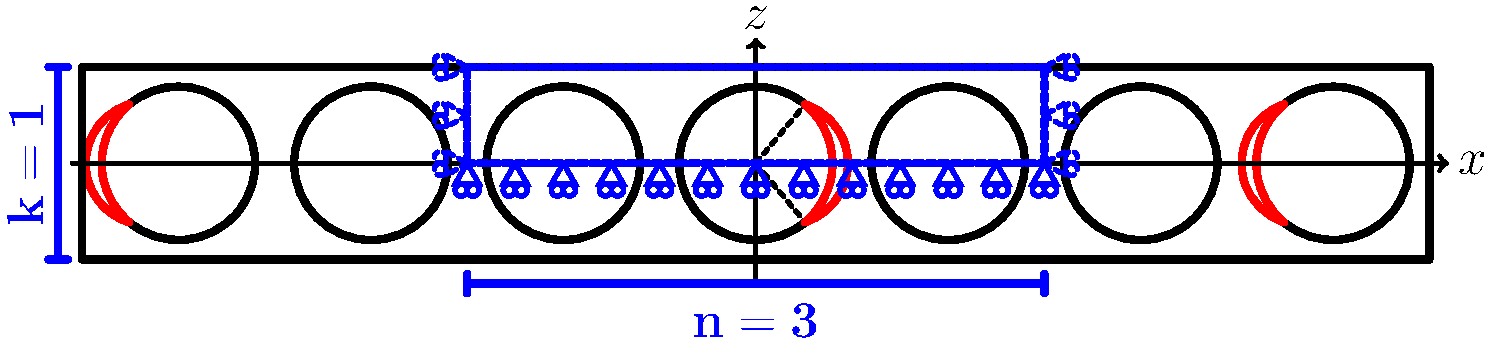
\includegraphics[width=\textwidth]{paperB/freeThinPly.pdf}
        \caption{Single row of fibers with a debond appearing every $n$ fibers: model $n\times1-free$ ($n=3$ in the figure).}\label{paperB:subfig:freethinply}
    \end{subfigure}

    \begin{subfigure}[b]{0.9\textwidth}
        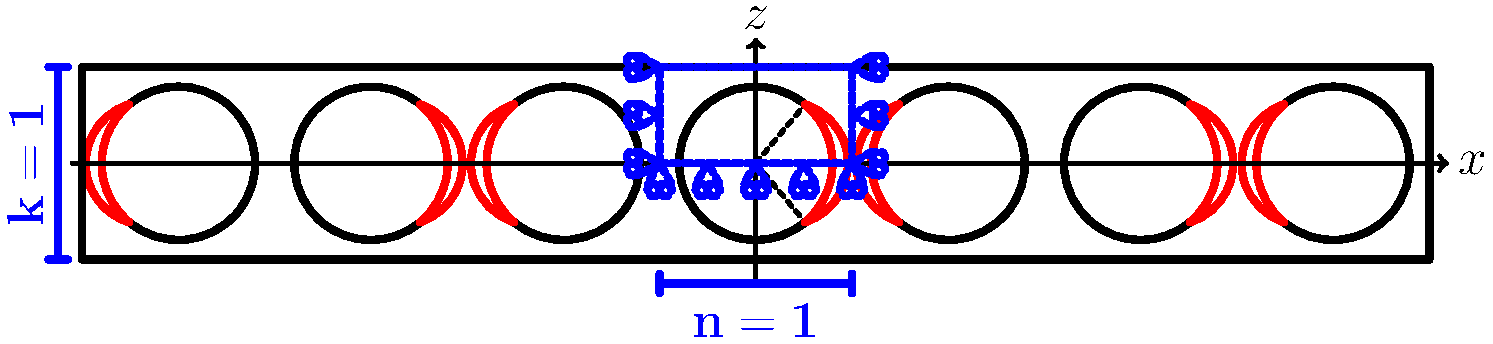
\includegraphics[width=\textwidth]{paperB/freeThinPlyAllDebonds.pdf}
        \caption{Single row of fibers with debonds appearing on each fiber: model $1\times1-free$ .}\label{paperB:subfig:freethinplyalldebonds}
    \end{subfigure}

\caption{Models of ultra-thin UD composites with a single ``row'' of fibers and debonds repeating at different distances.}\label{paperB:fig:laminateModelsA}
\end{figure}

In the sub-model of Fig.~\ref{paperB:subfig:freethinply}, every $n^{th}$ fiber in the composite is partially debonded on alternating sides of the fiber. The symmetries of the model allow the use of the upper part of the RUC, as highlighted in Fig.~\ref{paperB:fig:laminateModelsA} to~\ref{paperB:fig:thickplyalldebonds}. Following the notation introduced in Section~\ref{paperB:subsec:names}, we will refer to this model as $n\times 1-free$. In the sub-model $n=1$, Fig.~\ref{paperB:subfig:freethinplyalldebonds}, a debond appears on each fiber on alternating sides and the corresponding RUC contains only one fiber. We will refer to this model as $1\times 1-free$.

\begin{figure}[!h]
\centering
    \begin{subfigure}[b]{0.9\textwidth}
    \centering
        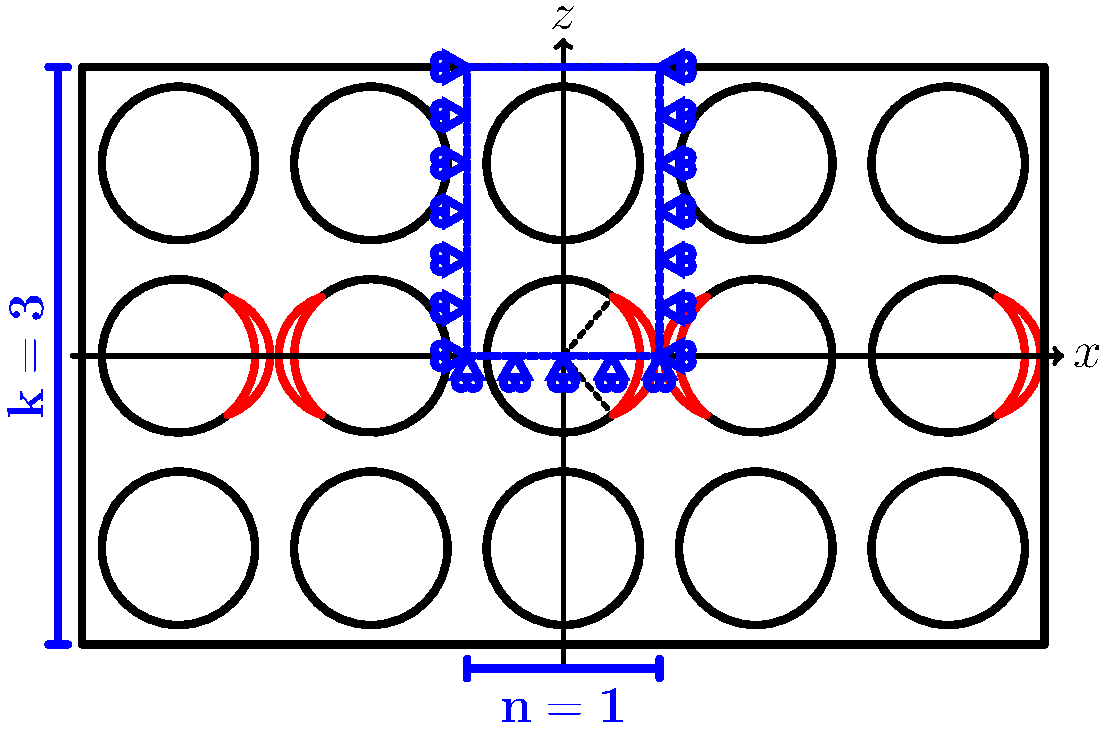
\includegraphics[height=0.3\textheight]{paperB/thickPlycentraldebondsline.pdf}
        \caption{Multiple rows of fibers with debonds appearing on each fiber beloging to the central row: model $1\times k-free$ ($k=3$ in the figure).}\label{paperB:subfig:thickplycentraldebonds}
    \end{subfigure}

    \begin{subfigure}[b]{0.9\textwidth}
        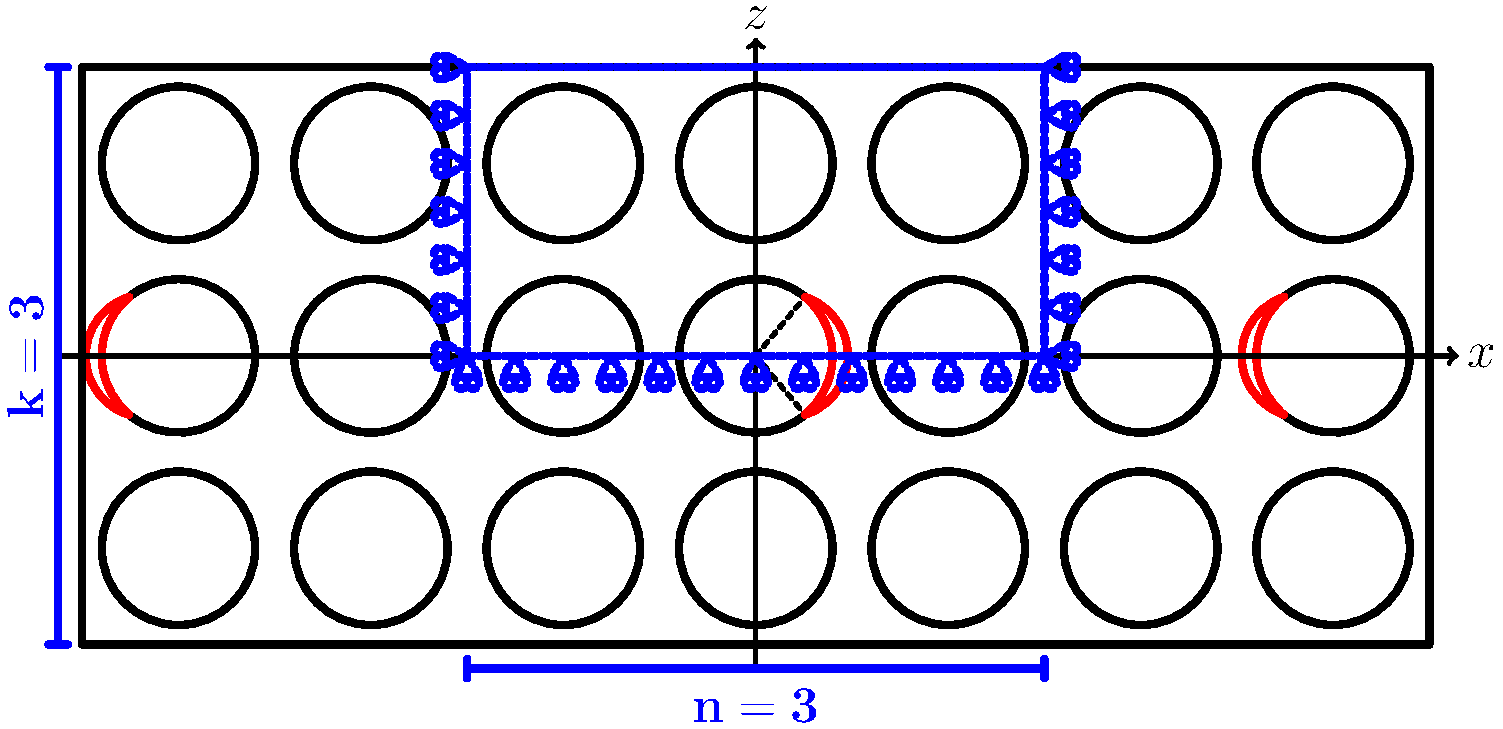
\includegraphics[width=\textwidth]{paperB/thickPly.pdf}
        \caption{Mutiple rows of fibers with a debond appearing every $n$ fibers within the central row: model $n\times k-free$ ($n=3$ and $k=3$ in the figure).}\label{paperB:subfig:thickply}
    \end{subfigure}

\caption{Models of UD composites with different ``rows'' of fibers and debonds repeating at different distances.}\label{paperB:fig:laminateModelsB}
\end{figure}

The second set of models in Fig.~\ref{paperB:fig:laminateModelsB} and Fig.~\ref{paperB:fig:thickplyalldebonds} considers laminates with multiple rows of fibers across the thickness: a finite number of rows in the first two sub-models in Fig.~\ref{paperB:fig:laminateModelsB}; an infinite number in the model of Fig.~\ref{paperB:fig:thickplyalldebonds}. In Fig. ~\ref{paperB:subfig:thickplycentraldebonds}, the RUC contains $n=1$ fiber in the x-direction, $k$ fibers across the thickness and the central fiber is debonded. This model will be referred to in the following as $1\times k-free$. Thinking in terms of rows, in this model we have a central row where each fiber is debonded. This row is surrounded from each side by $\nicefrac{\left(k-1\right)}{2}$ rows with perfectly bonded fibers. In the sub-model in Fig.~\ref{paperB:subfig:thickply}, each $n^{th}$ fiber in the central row is debonded and this row is surrounded by $\nicefrac{\left(k-1\right)}{2}$ rows of undamaged fibers from each side. We will refer to this model as $n\times k-free$ (because the horizontal boundary of the RUC is free of any constraint).

\begin{figure}[!h]
\centering
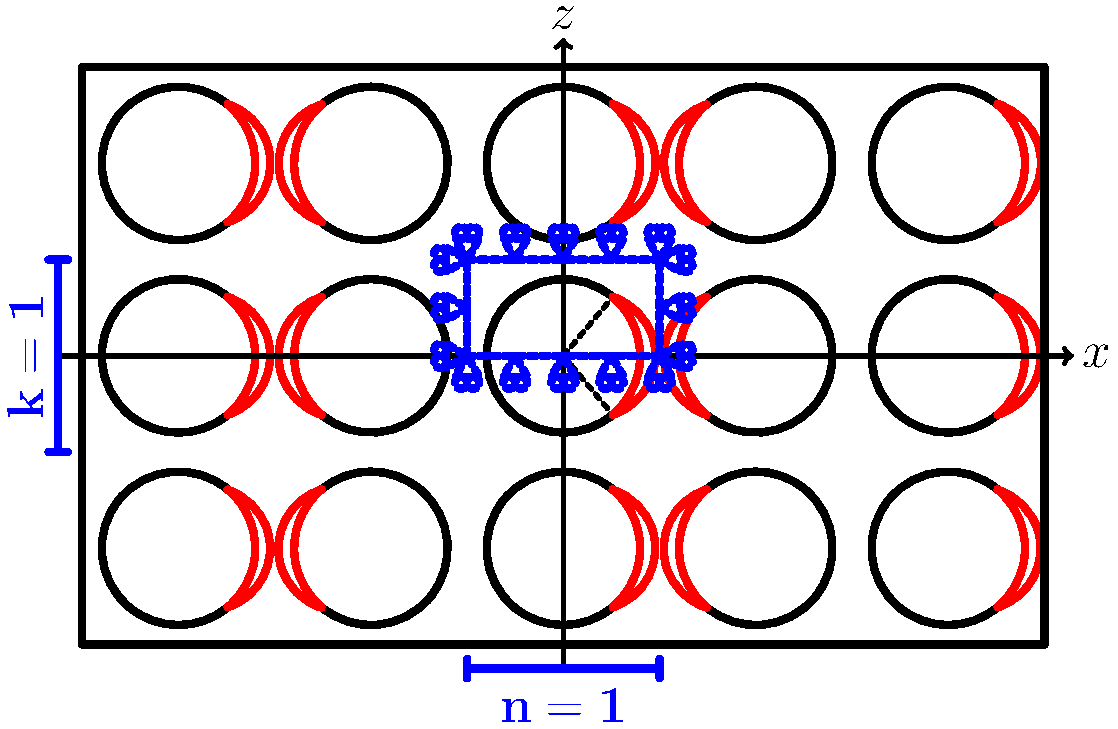
\includegraphics[width=0.9\textwidth]{paperB/thickPlyAllDebonds.pdf}
\caption{Model of UD composites with an infinite number of  ``rows'' of fibers and debonds appearing on each fiber: model $1\times1-coupling$ .}\label{paperB:fig:thickplyalldebonds}
\end{figure}

Finally, the model in Fig.~\ref{paperB:fig:thickplyalldebonds} represents an UD composite with an infinite number of rows; all of them with partially debonded fibers. As all fibers have debonds, the corresponding RUC is made of a single partially debonded fiber with kinematic coupling conditions applied to the upper boundary to assure periodicity. This model is referred to as $1\times 1-coupling$.

%\begin{table}[!h]
% \centering
% \caption{Summary of the models and their characteristics.}
% \begin{tabularx}{\textwidth}{p{0.05\textwidth}ccccc}
%\multicolumn{2}{c}{\textbf{Name}} & \multicolumn{4}{c}{\textbf{Boundary conditions}}\\
%                                                         &  & Up & Down & Right & Left \\
%\toprule
%\midrule
%\multicolumn{2}{c}{$\mathbf{D\left(m+1\right)H0V1L}$} &x-symmetry&free&coupling,&coupling,\\
%                                                         &  &  &  & $\bar{\varepsilon}_{x}=1\%$ & $\bar{\varepsilon}_{x}=1\%$ \\
%&\multicolumn{5}{X}{\small A debond every $\left(m+1\right)^{th}$ fiber in the horizontal direction, in a UD composites with 1 layer of fibers, Fig.~\ref{paperB:subfig:freethinply}.}\\
%\midrule
%\multicolumn{2}{c}{$\mathbf{D1H0V1L}$} &x-symmetry&free&coupling,&coupling,\\
%                                                         &  &  &  & $\bar{\varepsilon}_{x}=1\%$ & $\bar{\varepsilon}_{x}=1\%$ \\
%&\multicolumn{5}{X}{\small A debond every $1^{st}$ fiber in the horizontal direction, in a UD composites with 1 layer of fibers, Fig.~\ref{paperB:subfig:freethinplyalldebonds}.}\\
%\midrule
%\multicolumn{2}{c}{$\mathbf{D1H0V\left(2p+1\right)L}$} &x-symmetry&free&coupling,&coupling,\\
%                                                         &  &  &  & $\bar{\varepsilon}_{x}=1\%$ & $\bar{\varepsilon}_{x}=1\%$ \\
%&\multicolumn{5}{X}{\small A debond every $1^{st}$ fiber in the horizontal direction, in a UD composites with $\left(2p+1\right)$ layer of fibers, Fig.~\ref{paperB:subfig:thickplycentraldebonds}.}\\
%\midrule
%\multicolumn{2}{c}{$\mathbf{D\left(m+1\right)H0V\left(2p+1\right)L}$} &x-symmetry&free&coupling,&coupling,\\
%                                                         &  &  &  & $\bar{\varepsilon}_{x}=1\%$ & $\bar{\varepsilon}_{x}=1\%$ \\
%&\multicolumn{5}{X}{\small A debond every $\left(m+1\right)^{th}$ fiber in the horizontal direction, in a UD composites with $\left(2p+1\right)$ layers of fibers, Fig.~\ref{paperB:subfig:thickply}.}\\
%\midrule
%\multicolumn{2}{c}{$\mathbf{D1H1V\infty L}$} &x-symmetry&coupling&coupling,&coupling,\\
%                                                         &  &  &  & $\bar{\varepsilon}_{x}=1\%$ & $\bar{\varepsilon}_{x}=1\%$ \\
%&\multicolumn{5}{X}{\small A debond every $1^{st}$ fiber in the horizontal direction and every $1^{st}$ fiber in the vertical direction, in a UD composites with an infinite number of  layers of fibers, Fig.~\ref{paperB:fig:thickplyalldebonds}.}\\
%\bottomrule
%\end{tabularx}
%\label{paperB:tab:modelcharacteristics}
%\end{table}
%
%A summary of models' names and characteristics is reported in Table~\ref{paperB:tab:modelcharacteristics}

\subsection{Finite Element (FE) discretization}

Each RUC is discretized using the Finite Element Method (FEM) within the Abaqus environment, a commercial FEM package~\cite{abq12}. The length $l$ and height $h$ of the model are determined by the number of fibers $n$ in the horizontal direction and $k$ across the thickness (see~\ref{paperB:subsec:rve}) according to Eq.~\ref{paperB:eq:lengthheight}:

\begin{equation}\label{paperB:eq:lengthheight}
l=2nL\qquad h=kL;
\end{equation}

where $2L$ is the length of a one-fiber unit, see Fig.~\ref{paperB:subfig:modelschem}, defined as a function of the fiber volume fraction $V_{f}$ and the fiber radius according to

\begin{equation}\label{paperB:eq:LVf}
L=\frac{R_{f}}{2}\sqrt{\frac{\pi}{V_{f}}}.
\end{equation}

The fiber radius $R_{f}$ is assumed to be the same for each fiber in the model and equal to $1\ \mu m$. The latter value is not physical and it has been chosen for simplicity. It is worth to note at this point that, in a linear elastic solution as the one presented here, the ERR is proportional to the geometrical dimensions and recalculation of the ERR for fibers of any size, thus, requires a simple multiplication. Furthermore, notice that the relationships in Eqs.~\ref{paperB:eq:lengthheight} and~\ref{paperB:eq:LVf} ensure that the local and global $V_{f}$ are everywhere equal.

\begin{figure}[!h]
\centering
    %\begin{subfigure}[b]{0.55\textwidth}
        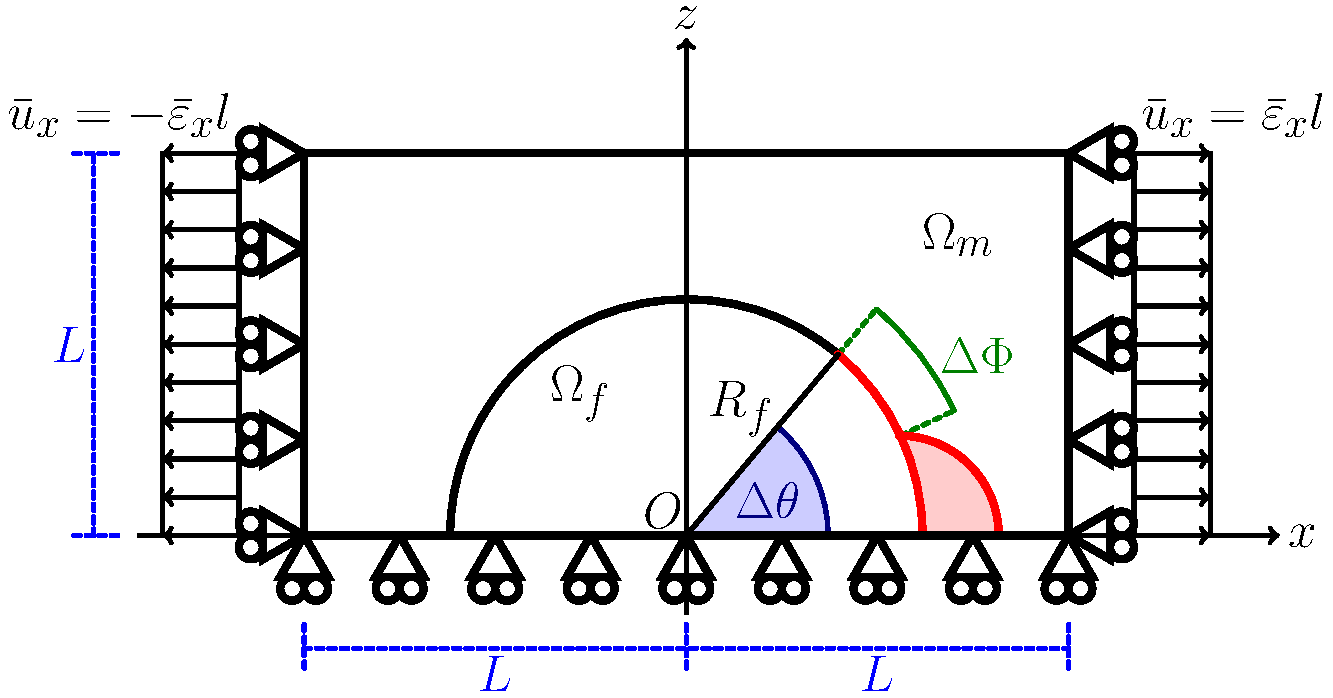
\includegraphics[width=0.9\textwidth]{paperB/RUC.pdf}
        %\caption{Schematic of the model with its main parameters.}\label{paperB:subfig:modelschem}
    %\end{subfigure} ~
    %\begin{subfigure}[b]{0.4\textwidth}
        %\includegraphics[width=\textwidth]{paperB/mesh-detail.eps}
       % \caption{Mesh near the crack tip. Crack's faces shown in red.}\label{paperB:subfig:meshdetail}
    %\end{subfigure}

\caption{Schematic of the model with its main parameters.}\label{paperB:subfig:modelschem}
\end{figure}

The debond is placed symmetrically with respect to the $x$ axis (see Fig.~\ref{paperB:subfig:modelschem}) and we characterize it with an angular size of $\Delta\theta$ (the full debond size is thus $2\Delta\theta$). For large debond sizes ($\geq 60^{\circ}-80^{\circ}$), a region of variable size $\Delta\Phi$ appears at the crack tip in which the crack faces are in contact and slide on each other. Due to its appearance, frictionless contact is considered between the two crack faces to allow free sliding and avoid interpenetration. The presence of friction at the interface is considered in~\cite{Varna1997}, where the authors model the contact interaction between crack faces using Coulomb's friction with a coefficient $\mu=0.25$ and show that, for a debond with $\Delta\theta=80^{\circ}$, the crack sliding displacement is always different from zero in every point of the crack and only slightly lower than that of the frictionless case. This in turn means that the estimation of $G_{II}$ in the case of frictionless contact provide an upper bound and thus the results presented here represent a conservative estimation (a higher ERR corresponds to higher likelihood of crack propagation). Symmetry with respect to the $x$ axis is applied on the lower boundary. The upper boundary is in general free, except for the model $1\times 1-coupling$ (Fig.~\ref{paperB:fig:thickplyalldebonds}) which requires kinematic coupling of vertical displacements also on the upper side. Kinematic coupling on the $x$-displacement is applied along the left and right sides of the model in the form of a constant $x$-displacement $\pm\bar{\varepsilon}_{x} l$, corresponding to transverse strain $\bar{\varepsilon}_{x}$ equal to $1\%$.

\begin{table}[!htbp]
 \centering
 \caption{Summary of the mechanical properties of fiber and matrix. $E$ stands for Young's modulus, $\mu$ for shear modulus and $\nu$ for Poisson's ratio.}
 \begin{tabular}{cccc}
\\
\textbf{Material} & \textbf{$E\left[GPa\right]$}\ & \textbf{$\mu\left[GPa\right]$} & \textbf{$\nu\left[-\right]$} \\
\midrule
Glass fiber    & 70.0  & 29.2   & 0.2  \\
Epoxy    & 3.5    & 1.25   & 0.4
\end{tabular}
\label{paperB:tab:phaseprop}
\end{table}

The model is meshed using second order, 2D, plane strain triangular (CPE6) and rectangular (CPE8) elements, which have respectively $6$ and $8$ nodes per element. Each node has $2$ degrees of freedom, i.e. the horizontal displacement $u_{x}$ and the vertical displacement $u_{z}$. A regular mesh of quadrilateral elements with an almost unitary aspect ratio is required at the crack tip. The angular size $\delta$ of an element in the crack tip region is always equal to $0.05^{\circ}$. The overall number of elements needed to discretize the model depends on the debond size $\Delta\theta$ (larger debonds have larger contact zones which require more elements for their correct resolution), the fiber volume fraction (which determines the size of the RVE) and the number of fully bonded fibers present in the model. As an example, the discretization of the $1\times 1-free$ model at $V_{f}=60\%$ requires a total of $132507$ elements for $\Delta\theta=10^{\circ}$ and of $296606$ elements for $\Delta\theta=140^{\circ}$, which corresponds to a minimum required RAM respectively of $445\ MB$ and $1014\ MB$ and to a minimum RAM needed to minimize I/O operations respectively of $1.63\ GB$ and $3.87\ GB$. To put it into perspective, the wallclock time required for their solution is respectively  $1.3\ \left[min\right]$ and $14.95\ \left[min\right]$ on a laptop with a $2.5\ GHz$ Intel Core i5 processor and $6\ GB$ of installed RAM. The crack faces are modeled as element-based surfaces and a small-sliding contact pair interaction with no friction is established between them. The Mode I, Mode II and total Energy Release Rates (ERRs) (respectively referred to as $G_{I}$, $G_{II}$ and $G_{TOT}$) represent the main output of the FEM analysis; they are evaluated using the VCCT~\cite{Krueger2004} implemented in a custom Python routine and, for the total ERR, the J-integral~\cite{Rice1968} is obtained by application of the Abaqus built-in functionality. A glass fiber-epoxy system is considered throughout this paper, and it is assumed that their response lies always in the linear elastic domain. The latter assumption lies on the work of Asp and co-workers, who show that epoxy subjected to a tri-axial stress state as the one observable in the inter-fibers region fails at very low strains ($\sim0.5\%-0.8\%$)~\cite{Asp1995} and in a brittle manner~\cite{Asp1996}, and that the magnitude of deviatoric stresses (evaluated in terms of equivalent Von Mises stress) in the fiber/matrix interface neighborhood does not justify the occurrence of plastic deformations in the case of debond propagation~\cite{Asp1996}. The properties used are listed in Table~\ref{paperB:tab:phaseprop}.

\subsection{Validation of the model}

The model is validated in Fig.~\ref{paperB:fig:validation} against the results reported in~\cite{Paris2007,Sandino2016}, obtained with the Boundary Element Method (BEM) for a single fiber with a symmetric debond placed in an infinite matrix. This situation is modeled using the $1\times1-free$ RVE with $V_{f}=0.0079\%$, which corresponds to a RUC's length and height of respectively $\sim 200R_{f}$ and $\sim 100R_{f}$.

\begin{figure}[!h]
\centering
\includegraphics[width=0.9\textwidth]{paperB/validation-VCCT.pdf}
\caption{Validation of the single fiber model for the infinite matrix case with respect to the BEM solution in \cite{Sandino2016}.}\label{paperB:fig:validation}
\end{figure}

To allow for a comparison, the results are normalized following~\cite{Sandino2016} with respect to a reference Energy Release Rate $G_{0}$ defined as

\begin{equation}
G_{0}=\frac{1+k_{m}}{8\mu_{m}}\sigma_{0}^{2}\pi R_{f}
\end{equation}

where $\mu$ is the shear modulus, $k$ is the Kolosov's constant defined as $3-4\nu$ for plane strain conditions, $R_{f}$ is the fiber radius and the index $m$ refers to the properties of the matrix. $\sigma_{0}$ is the stress at the boundary, computed as the average of the stress extracted at each boundary node along the right side (arithmetic average as nodes are equispaced by design along both the left and right sides). The agreement is good: the difference between the BEM solution, which is considered more accurate, and the FEM solution does not exceed $5\%$. The ERRs' maxima are in the same positions and the size of the contact zone is the same.  Nevertheless, an analysis of phenomena leading to less than $5\%$ differences in ERR would not be reliable and, therefore, it is not recommended.

%%%%%%%%%%%%%%%%%%%%%%%%%%%%%%%%%%%%%%%%%%%%%%%%%%%%%%%%%%%%%%%%%%%
%%%%%%%%%%%%%%%%%%%%%%%%%%%%%%%%%%%%%%%%%%%%%%%%%%%%%%%%%%%%%%%%%%%

\section{Results \& Discussion}

\subsection{Effect of Fiber Volume Fraction}\label{paperB:subsec:volfrac}

As shown in Figs.~\ref{paperB:fig:volumefractionMI} and~\ref{paperB:fig:volumefractionMII}, respectively for Mode I and Mode II, the fiber content has a drastic effect on the Energy Release Rate at the tip of the fiber/matrix interface crack. The effect of four levels of fiber volume fraction are compared, $30\%$, $50\%$, $60\%$ and $65\%$, on two microstructural models: a $11\times 11-free$ (every $11^{th}$ fiber in the central fiber row is partially debonded and, on the top of this row, we have 5 undamaged fiber rows), Figs.~\ref{paperB:subfig:volfracsmallerMI} and~\ref{paperB:subfig:volfracsmallerMII}, and a $21\times 21-free$ (every $21^{th}$ fiber in the central fiber row is partially debonded and, on the top of this row, we have 10 undamaged fiber rows), Figs.~\ref{paperB:subfig:volfracbiggerMI} and~\ref{paperB:subfig:volfracbiggerMII}.

\begin{figure}[!h]
\centering
    \begin{subfigure}[b]{0.45\textwidth}
        \includegraphics[width=\textwidth]{paperB/vf-smallermodel-GI.pdf}
        \caption{Model $11\times 11-free$.}\label{paperB:subfig:volfracsmallerMI}
    \end{subfigure} ~
    \begin{subfigure}[b]{0.45\textwidth}
        \includegraphics[width=\textwidth]{paperB/vf-biggermodel-GI.pdf}
        \caption{Model $21\times 21-free$.}\label{paperB:subfig:volfracbiggerMI}
    \end{subfigure}

\caption{A view of the effect of fiber volume fraction on Mode I ERR in two exemplificative models, subject to an applied transverse strain $\varepsilon_{x}$ of $1\%$.}\label{paperB:fig:volumefractionMI}
\end{figure}

Comparing Fig.~\ref{paperB:subfig:volfracsmallerMI} with~\ref{paperB:subfig:volfracbiggerMI}, and Fig.~\ref{paperB:subfig:volfracsmallerMII} with~\ref{paperB:subfig:volfracbiggerMII}, we can observe that the ERRs' values are very similar for RUCs with $11\times11$ and $21\times21$ fibers, though they are slightly higher for the larger RUC where the next debonded fiber and the free surface are further away from the debonded fiber. From these results we conclude that both RUCs are large enough to represent a single debonded fiber in an infinite array of bonded fibers. Obviously, there exists a specific effect of the fiber content. For Mode I, Fig.~\ref{paperB:fig:volumefractionMI}, the maximum value of the ERR increases by $\sim 5.2$ times when $V_{f}$ changes from $30\%$ to $65\%$. The debond's angular size for which the peak value occurs remains unchanged at $20^{\circ}$, but for $V_{f}=60\%$ and $65\%$ the values of Mode I ERR are rather similar when measured at $10^{\circ}$ and at $20^{\circ}$, approximately creating a plateau. Furthermore, increasing the fiber volume fraction delays the onset of the contact zone, which corresponds in Fig.~\ref{paperB:fig:volumefractionMI} to the first value of $\Delta\theta$ for which $G_{I}$ is equal to zero. For $V_{f}=30\%$, the contact zone first appears for a debond of $60^{\circ}$, similarly to what happens in the single fiber in infinite matrix model (Fig.~\ref{paperB:fig:validation}). For higher fiber contents, the contact zone's onset is delayed to a debond's size approximately equal to $70^{\circ}$.

\begin{figure}[!h]
\centering
    \begin{subfigure}[b]{0.45\textwidth}
        \includegraphics[width=\textwidth]{paperB/vf-smallermodel-GII.pdf}
        \caption{Model $11\times 11-free$.}\label{paperB:subfig:volfracsmallerMII}
    \end{subfigure} ~
    \begin{subfigure}[b]{0.45\textwidth}
        \includegraphics[width=\textwidth]{paperB/vf-biggermodel-GII.pdf}
        \caption{Model $21\times 21-free$.}\label{paperB:subfig:volfracbiggerMII}
    \end{subfigure}

\caption{A view of the effect of fiber volume fraction on Mode II ERR in two exemplificative models, subject to an applied transverse strain $\varepsilon_{x}$ of $1\%$.}\label{paperB:fig:volumefractionMII}
\end{figure}

For Mode II, Fig.~\ref{paperB:fig:volumefractionMII}, there is a distinct maximum in the curve and its shape does not depend on the fiber content. The maximum value of the ERR increases by $\sim 2.1$ times when $V_{f}$ changes from $30\%$ to $65\%$. The effect is thus similar to Mode I, but with a significantly lower magnitude. Similar to Mode I, the debond size for which the peak value of Mode II occurs remains unchanged, at $60^{\circ}$. It is worthwhile to notice that the ratio of Mode II to Mode I peak values is $\frac{max\left(G_{II}\right)}{max\left(G_{I}\right)}\sim\frac{2.2}{0.9}\sim 2.4$ for $V_{f}=30\%$, while it is $\sim\frac{4.7}{4.7}\sim 1$ for $V_{f}=65\%$.\\% Given that the peaks occur at different debond's sizes, for which the value of the other ERR is very small or even close to zero, this means that the increase in fiber content creates a long range of very close values of the total ERR, that may have a global destabilizing effect on debond growth.\\
The general increasing trends observed in Figs.~\ref{paperB:fig:volumefractionMI} and~\ref{paperB:fig:volumefractionMII} are related to the fact that, given that the global and local $V_{f}$ are everywhere identical in the models presented, an increase in fiber content corresponds to a decrease in the average distance between fibers. Thus, the distances for the decay of the local stress and strain fields in the matrix domain become shorter, leading to higher stresses in general and causing higher values at the crack tip. The difference in relative magnitude between Mode I and Mode II and the delay in the contact zone's onset are instead due to the interplay between two different mechanisms, both caused by the ordered microstructural arrangement of the model. In the models considered, a fully bonded fiber is always placed along the horizontal direction, aligned with the partially debonded fiber and exactly in front of the debond. By increasing $V_{f}$, the former moves closer to the latter and for small debonds this causes a magnification of the x-strain at the crack tip. For small debonds ($\leq 20^{\circ}-30^{\circ}$) in fact, the crack tip is approximately normal to the $x$-direction and thus an increase in $\varepsilon_{x}$ causes an increase in $G_{I}$. On the other hand, for large debonds ($\geq 70^{\circ}-80^{\circ}$) the crack growth direction is almost aligned with the $x$-axis, thus a magnification in the $x$-strain translates into an increase of Mode II ERR. However, this increasing effect on $G_{II}$ is partially counteracted by the presence of a fully bonded fiber on top of the debonded fiber and aligned with it. As fibers are more rigid than the surrounding matrix, the presence of the former will restrain horizontal displacements, thus hampering strong increases in $G_{II}$ for large debonds. Furthermore, due to the mismatch in the Poisson's ratios, the fully bonded fiber placed above generates an upward-directed component of the vertical displacement field in the matrix, which tends to open the debond and causes the delay in the contact zone's onset. The interplay between these mechanisms is governed by the average inter-fiber distance and, in turn, by the fiber volume fraction.\\
These observations are in agreement with the results reported in~\cite{Sandino2016}, where the effect on the ERR of a partially debonded fiber of two fully bonded nearby fibers, placed symmetrically with respect to the loading direction, is studied for different angular positions (denoted as $\theta_{2}$) and radial distances in a model with an effectively infinite matrix ($V_{f}\sim0.09\%$). The effect of the former is studied for a constant value of the radial distance between the debonded and bonded fibers, which corresponds to a local $V_{f}^{local}$ of $\sim62\%$ assuming hexagonal packing. They report an increase in both Mode I and Mode II ERR with respect to the single fiber case when the two fibers are placed at an angle of respectively $\pm25^{\circ},\pm30^{\circ},\pm140^{\circ},\pm150^{\circ},\pm155^{\circ}$, i.e. closest to the loading direction. Notice that for $\pm25^{\circ}$ and $\pm155^{\circ}$ the two fully bonded fibers are almost in contact, with an inter-fiber distance of $\sim0.04$ times their radius. This result confirms the considerations made in the previous paragraph about the $x$-strain magnification caused by the presence of fully bonded fibers along the loading direction. The effect is further analyzed and discussed in Sec.~\ref{paperB:subsec:singlefiberud} and Sec.~\ref{paperB:subsec:multrow}. In the range $\pm40^{\circ}-\pm130^{\circ}$ instead, the presence of the other fibers causes a reduction of the ERR and, particularly in the range $80^{\circ}-120^{\circ}$, results are very close and almost insensitive to variations in $\theta_{2}$, which supports the previous conclusion about the effect of a fully bonded fiber on top the partially debonded one. This effect is treated in more detail in Sec.~\ref{paperB:subsec:fiberabove}.\\
Comparing the results from~\cite{Sandino2016} with those presented in this paper, an hypothesis can be furthermore formulated about the robustness of the results of the present article with respect to deviations in fiber position: it seems reasonable to assume a tolerance to deviations of max. $\pm30^{\circ}$ with respect to the loading direction and of max. $\pm20^{\circ}$ with respect to the through-the-thickness direction.\\
The effect of the local fiber content is also investigated in~\cite{Sandino2016}, by changing the radial distance between the partially debonded fiber and the fully bonded ones. They observe that the further the fully bonded fibers are placed from the central one, i.e. the lower the local $V_{f}$, the lower is their effect on the ERR. The magnitude of the effect is however small: the maximum increase of the total ERR is of $\sim1.15$ times for $\theta_{2}=30^{\circ}$ and $150^{\circ}$ when increasing $V_{f}^{local}$ from $28\%$ to $62\%$; the total ERR decreases by a factor of $\sim0.62$ for $\theta_{2}=60^{\circ}$, $\sim0.74$ for $\theta_{2}=90^{\circ}$ and $\sim0.5$ for $\theta_{2}=120^{\circ}$ when increasing $V_{f}^{local}$ from $28\%$ to $62\%$. Analogous results can be found in~\cite{Zhuang2018}, where the authors consider a centrally-placed partially debonded fiber sorrounded by an hexagonal cluster inside an homogenized UD composite. They observe a reduction in the ERR when the local fiber volume fraction is increased, i.e. when the spacing between fibers is reduced. The strongest change is reported for Mode II, which decreases by a factor of $\sim0.73$ when the local fiber volume fraction is decreased from $66\%$ to $78\%$. Thus, the trends presented in~\cite{Sandino2016,Zhuang2018} are in agreement with our results on the effect of $V_{f}$ and support the considerations made so far. The stark difference in magnitude however highlights the contrast between the effect of the local fiber volume fraction of a cluster of fibers inside an infinite medium and of the global $V_{f}$ of long-range microstructural arrangements, such the ones considered in this article. The similarity in trends with the concurrent difference in magnitudes can be explained in relation to the characteristics of the elastic solution computed. In the first case the local fiber volume fraction controls the distance, with respect to the central partially debonded fiber, at which a localized perturbation zone appears in the far-field elastic solution; in the second case the global $V_{f}$ determines the characteristic lengths of a global periodic solution.

\subsection{Interaction between debonds in UD composites with a single row of fibers}\label{paperB:subsec:singlefiberud}

The interaction of debonds appearing at regular intervals in an ultra-thin UD composite with a single row of fibers is studied for Mode I (Fig.~\ref{paperB:fig:sidefibersMI}) and Mode II (Fig.~\ref{paperB:fig:sidefibersMII}) and fiber content equal to $30\%$ (Figs.~\ref{paperB:subfig:sidefiber30MI} and~\ref{paperB:subfig:sidefiber30MII}) and $60\%$ (Figs.~\ref{paperB:subfig:sidefiber60MI} and~\ref{paperB:subfig:sidefiber60MII}). The models treated are $3\times 1-free$, $5\times 1-free$, $7\times 1-free$, $11\times 1-free$, $21\times 1-free$, $101\times 1-free$ and $201\times 1-free$, corresponding respectively to a debond every $3^{rd}$, $5^{th}$, $7^{th}$, $11^{th}$, $21^{st}$, $101^{st}$ and $201^{st}$ fiber (Fig.~\ref{paperB:subfig:freethinply}). Given that the upper surface of the UD row is left free, the interaction with the debonded fiber in the next RUC is stronger than in any other case and the results of this section are thus the most conservative in terms of debond's growth: the ERRs should be the largest. The effect is enhanced in composites with high $V_{f}$ and especially for $G_{II}$: at $V_{f}=60\%$ the highest $G_{II}$ value for the $201\times 1-free$ composite in Fig.~\ref{paperB:subfig:sidefiber60MII} is more than $3$ times higher than the $G_{II}$ value value for the $21\times21-free$ composite in Fig.~\ref{paperB:subfig:volfracbiggerMII}. Even the maximum is shifted to larger angles. The $G_{I}$ value is for some cases only 30\% higher.\\
From both Fig.~\ref{paperB:fig:sidefibersMI} and Fig.~\ref{paperB:fig:sidefibersMII}, it can be seen that the presence of a debond close to the analyzed debond decreases the strain magnification effect discussed in Sec.~\ref{paperB:subsec:volfrac} and thus reduces the value of the ERR. This phenomenon is called ``crack shielding''~\cite{Garcia2015}.

\begin{figure}[!h]
\centering
    \begin{subfigure}[b]{0.45\textwidth}
        \includegraphics[width=\textwidth]{paperB/sidefibers-vf30-GI.pdf}
        \caption{$V_{f}=30\%$.}\label{paperB:subfig:sidefiber30MI}
    \end{subfigure} ~
    \begin{subfigure}[b]{0.45\textwidth}
        \includegraphics[width=\textwidth]{paperB/sidefibers-vf60-GI.pdf}
        \caption{$V_{f}=60\%$.}\label{paperB:subfig:sidefiber60MI}
    \end{subfigure}

\caption{Effect of the interaction between debonds appearing at regular intervals on Mode I ERR in an UD with a single row of fibers at different levels of fiber volume fraction $V_{f}$, subject to an applied transverse strain $\varepsilon_{x}$ of $1\%$.}\label{paperB:fig:sidefibersMI}
\end{figure}

For Mode I, the presence of a free surface, and inversely the absence of a fully bonded fiber along the vertical direction, implies the absence of the counteracting upward-oriented vertical component of the displacement field due to the mismatch in Poisson's ratios. This in turn translates into the constancy of the value of $\Delta\theta$ corresponding to contact zone's onset, always equal to $60^{\circ}$. For $V_{f}=30\%$, Mode I is reduced when the spacing between debonds (in terms of number of fully bonded fibers between them in our models) decreases, but the magnitude of change is significant only in the range when the spacing is reduced from a debond every $5^{th}$ fiber to one every $3^{rd}$. For comparison, the difference of peak $G_{I}$ values for $V_{f}=30\%$ between $5\times 1-free$ and $3\times 1-free$ is $\sim 0.2\ \frac{J}{m^{2}}$ (around $30\%$ of the lower value), while between $201\times 1-free$ and $5\times 1-free$ is $\sim 0.05\ \frac{J}{m^{2}}$ (around $7\%$ of the lower value). A similar observation can be made for $V_{f}=60\%$, but for larger spacings: no difference can be seen between the case of a debond placed every $101^{st}$ and every $201^{st}$ fiber. These observations suggest the existence of characteristic distance dependent on the fiber volume fraction which governs the interaction between debonds: in low $V_{f}$ composites ($V_{f}=30\%$) the convergence to a non-interactive solution is faster (less interaction between debonded fibers in neighboring RUCs).

\begin{figure}[!h]
\centering
    \begin{subfigure}[b]{0.45\textwidth}
        \includegraphics[width=\textwidth]{paperB/sidefibers-vf30-GII.pdf}
        \caption{$V_{f}=30\%$.}\label{paperB:subfig:sidefiber30MII}
    \end{subfigure} ~
    \begin{subfigure}[b]{0.45\textwidth}
        \includegraphics[width=\textwidth]{paperB/sidefibers-vf60-GII.pdf}
        \caption{$V_{f}=60\%$.}\label{paperB:subfig:sidefiber60MII}
    \end{subfigure}

\caption{Effect of the interaction between debonds appearing at regular intervals on Mode II ERR in an UD with a single row of fibers at different levels of fiber volume fraction $V_{f}$, subject to an applied transverse strain $\varepsilon_{x}$ of $1\%$.}\label{paperB:fig:sidefibersMII}
\end{figure}

Without costraint on the upper surface, the strain magnification effect creates a larger displacement gap in the $x$-direction, which increases Mode II for larger debonds. When debonds are far apart, the series of rigid elements in the ultra-thin composite row (constituted by fully bonded fibers and their surrounding matrix) creates higher $x$-strains than in average in the element with the debonded fiber, which in turn generates higher tangential displacements at the crack tip for larger debonds. Conversely, when debonds are closer (smaller number of rigid elements between them), the strain concentration in the debonded element is more similar to the applied strain (the magnification is reduced) and the tangential displacement component at the crack tip decreases for large $\Delta\theta$. This is the mechanism behind the change in the value of $\Delta\theta$ for which the peak of $G_{II}$ occurs: from $70^{\circ}$ to $50^{\circ}$ at $30\%$, and from $80^{\circ}$ to $40^{\circ}$ at $60\%$ going from the higher to the smaller spacing of debonds. Differently from Mode I, the presence of a characteristic distance is harder to establish. For $V_{f}=30\%$ (Fig.~\ref{paperB:subfig:sidefiber30MII}), it seems reasonable to establish it at around $100$ fully bonded fibers between each debond. For $V_{f}=60\%$ (Fig.~\ref{paperB:subfig:sidefiber60MII}), the difference between models $101\times 1-free$ and $201\times 1-free$ is still sizable, thus preventing the establishment of such characteristic distance. It is possible to observe, however, that the change between $101\times 1-free$ and $201\times 1-free$ is significantly smaller than between $21\times 1-free$ and $101\times 1-free$ ($2\left[\frac{J}{m^{2}}\right]$ vs $11\left[\frac{J}{m^{2}}\right]$), thus suggesting the existence of the characteristic distance outside the range studied. Nevertheless, one should question whether the single row composite with free surface is an appropriate RUC for defining the upper bound for $G_{II}$: $G_{II}$ may be more affected by the free surface than by the effect of the interaction between debonds in the row.

\subsection{Influence of rows of fully bonded fibers on debond's ERR in the middle row}\label{paperB:subsec:fiberabove}

The effect of the presence of rows of fully bonded fibers on debond's growth in the central row with all fibers partially debonded is studied for Mode I (Fig.~\ref{paperB:fig:abovefibersMI}) and Mode II (Fig.~\ref{paperB:fig:abovefibersMII}) and fiber content equal to $30\%$ (Figs.~\ref{paperB:subfig:abovefiber30MI} and~\ref{paperB:subfig:abovefiber30MII}) and $60\%$ (Figs.~\ref{paperB:subfig:abovefiber60MI} and~\ref{paperB:subfig:abovefiber60MII}). The models treated are $1\times 3-free$, $1\times 5-free$, $1\times 7-free$, $1\times 11-free$, $1\times 21-free$, $1\times 101-free$ and $1\times 201-free$, corresponding to a UD composite with respectively $3$, $5$, $7$, $11$, $21$, $101$ and $201$ rows of fibers (Fig.~\ref{paperB:subfig:thickplycentraldebonds}).

\begin{figure}[!h]
\centering
    \begin{subfigure}[b]{0.45\textwidth}
        \includegraphics[width=\textwidth]{paperB/abovefibers-vf30-GI.pdf}
        \caption{$V_{f}=30\%$.}\label{paperB:subfig:abovefiber30MI}
    \end{subfigure} ~
    \begin{subfigure}[b]{0.45\textwidth}
        \includegraphics[width=\textwidth]{paperB/abovefibers-vf60-GI.pdf}
        \caption{$V_{f}=60\%$.}\label{paperB:subfig:abovefiber60MI}
    \end{subfigure}

\caption{Influence of rows of fully bonded fibers on debond's growth in Mode I ERR in a centrally located row of debonded fibers at different levels of fiber volume fraction $V_{f}$, subject to an applied transverse strain $\varepsilon_{x}$ of $1\%$.}\label{paperB:fig:abovefibersMI}
\end{figure}

The results shown strengthen the arguments made in Sec.~\ref{paperB:subsec:volfrac} and Sec.~\ref{paperB:subsec:singlefiberud}. It can, in fact, be seen in Fig.~\ref{paperB:fig:abovefibersMI} that an increasing number of bonded fiber rows across the thickness delays the onset of the contact zone to a debond of $70^{\circ}$ in size, due to the introduction of an additional positive component of the vertical displacement which translates into an opening displacement at the debond's tip.\\
Comparing Fig.~\ref{paperB:subfig:sidefiber60MII} with Fig.~\ref{paperB:subfig:abovefiber60MII}, we observe that the presence of bonded fiber rows significantly reduce the $G_{II}$ and its maximum is shifted back to $60^{\circ}$, thus confirming the hypothesis in Section~\ref{paperB:subsec:singlefiberud} that the absence of $G_{II}$ convergence with the increasing distance in a single-row composite is caused more by the free surface than by the interaction between debonds.

\begin{figure}[!h]
\centering
    \begin{subfigure}[b]{0.45\textwidth}
        \includegraphics[width=\textwidth]{paperB/abovefibers-vf30-GII.pdf}
        \caption{$V_{f}=30\%$.}\label{paperB:subfig:abovefiber30MII}
    \end{subfigure} ~
    \begin{subfigure}[b]{0.45\textwidth}
        \includegraphics[width=\textwidth]{paperB/abovefibers-vf60-GII.pdf}
        \caption{$V_{f}=60\%$.}\label{paperB:subfig:abovefiber60MII}
    \end{subfigure}

\caption{Influence of rows of fully bonded fibers on debond's growth in Mode II ERR in a centrally located row of debonded fibers at different levels of fiber volume fraction $V_{f}$, subject to an applied transverse strain $\varepsilon_{x}$ of $1\%$.}\label{paperB:fig:abovefibersMII}
\end{figure}

The results of both Mode I and Mode II show that the introduction of an increasing number of fully bonded fiber rows doesn't change the ERR calculated at the crack tip after adding more than one row (the convergence is very fast). A small effect, mostly on Mode I, of the number of bonded fiber rows can be observed at low fiber content (Figs.~\ref{paperB:subfig:abovefiber30MI} and~\ref{paperB:subfig:abovefiber30MII}), while for high fiber content the smaller model with only one fiber row above the partially debonded one is already representative.

\subsection{Effect of multiple rows of bonded fibers on debonding in the central row of a UD composite with different distances between debonded fibers}\label{paperB:subsec:multrow}

The ERR of debonds appearing at regular intervals in the central row of fibers in UD composites is affected by the number of rows with bonded fibers. The effect is investigated using different combinations of horizontal debond spacing, controlled by the number of bonded fibers in the central row of the RUC, and the number of rows of bonded fibers on top of it. The following models have been studied: $3\times 3-free$, $5\times 3-free$, $5\times 5-free$, $7\times 3-free$, $7\times 5-free$, $7\times 7-free$, $11\times 3-free$, $11\times 5-free$, $11\times 7-free$, $11\times 11-free$, $21\times 3-free$, $21\times 5-free$, $21\times 7-free$, $21\times 11-free$, $21\times 21-free$, $101\times 3-free$, $101\times 5-free$, $101\times 7-free$, $101\times 11-free$, $201\times 3-free$, $201\times 5-free$, $201\times 7-free$, $201\times 11-free$  (Fig.~\ref{paperB:subfig:thickply}).

\begin{figure}[!h]
\centering
    \begin{subfigure}[b]{0.45\textwidth}
        \includegraphics[width=\textwidth]{paperB/sideabovefibers-vf60-GI.pdf}
        \caption{$G_{I}$.}\label{paperB:subfig:sideabovefiber60MIsp}
    \end{subfigure} ~
    \begin{subfigure}[b]{0.45\textwidth}
        \includegraphics[width=\textwidth]{paperB/sideabovefibers-vf60-GII.pdf}
        \caption{$G_{II}$.}\label{paperB:subfig:sideabovefiber60MIIsp}
    \end{subfigure}

\caption{Effect on Mode I and Mode II ERR of the presence of an increasing number of rows of fully bonded fibers in UD composites with debonds appearing every $10^{th}$ fiber (model $21\times k-free$). $V_{f}=60\%$ and $\varepsilon_{x}=1\%$.}\label{paperB:fig:sideabovefibersspacingfixed}
\end{figure}

The results shown in Fig.~\ref{paperB:fig:sideabovefibersspacingfixed} confirm the observations discussed in Sec.~\ref{paperB:subsec:singlefiberud} and Sec.~\ref{paperB:subsec:fiberabove}: the presence of fully bonded fiber rows on top of the central row with debonded fibers reduces the interaction with the free surface and thus has a restraining effect on the ERR, that counteracts the magnification due to an increasing number of fully bonded fibers in the horizontal direction. The interplay is further modulated by the fiber content. Observing Fig.~\ref{paperB:fig:sideabovefibersspacingfixed}, it is possibe to note how the free surface interaction decays fast: the presence of 5 fiber rows across the thickness is already sufficient to prevent any significant effect of additional fiber rows on the ERR of a debond in the central row.

%Comparing with the results in Sec.~\ref{paperB:subsec:singlefiberud}, it can be observed how the presence of fully bonded fibers across the thickness has a restraining effect on the ERR, that counteracts the magnification due to an increasing number of fully bonded fibers in the horizontal direction. The interplay is further modulated by the fiber content. For Mode I, at low fiber content the contact zone onset starts at $60^{\circ}$, while it is delayed to debonds of $70^{\circ}$ for $V_{f}=60\%$.

%\begin{figure}[!h]
%\centering
%    \begin{subfigure}[b]{0.475\textwidth}
%        \includegraphics[width=\textwidth]{sideabovefibers-t3-vf60-GI.pdf}
%        \caption{$k=3$, $G_{I}$.}\label{paperB:subfig:sideabovefiber60MIt3}
%    \end{subfigure} ~
%    \begin{subfigure}[b]{0.475\textwidth}
%        \includegraphics[width=\textwidth]{sideabovefibers-t3-vf60-GII.pdf}
%        \caption{$k=3$, $G_{II}$.}\label{paperB:subfig:sideabovefiber60MIIt3}
%    \end{subfigure}
%
%    \begin{subfigure}[b]{0.475\textwidth}
%        \includegraphics[width=\textwidth]{sideabovefibers-t5-vf60-GI.pdf}
%        \caption{$k=5$, $G_{I}$.}\label{paperB:subfig:sideabovefiber60MIt5}
%    \end{subfigure} ~
%    \begin{subfigure}[b]{0.475\textwidth}
%        \includegraphics[width=\textwidth]{sideabovefibers-t5-vf60-GII.pdf}
%        \caption{$k=5$, $G_{II}$.}\label{paperB:subfig:sideabovefiber60MIIt5}
%    \end{subfigure}
%
%    \begin{subfigure}[b]{0.475\textwidth}
%        \includegraphics[width=\textwidth]{sideabovefibers-t11-vf60-GI.pdf}
%        \caption{$k=11$, $G_{I}$.}\label{paperB:subfig:sideabovefiber60MIt11}
%    \end{subfigure} ~
%    \begin{subfigure}[b]{0.475\textwidth}
%        \includegraphics[width=\textwidth]{sideabovefibers-t11-vf60-GII.pdf}
%        \caption{$k=11$, $G_{II}$.}\label{paperB:subfig:sideabovefiber60MIIt11}
%    \end{subfigure}
%
%\caption{Effect on Mode I and Mode II ERR of increasing the spacing between debonds appearing in the central row of fibers in a UD composite with a fixed number of rows across the thickness. $V_{f}=60\%$ and $\varepsilon_{x}=1\%$.}\label{paperB:fig:sideabovefibersthickfixed}
%\end{figure}

\begin{figure}[!h]
\centering
    \begin{subfigure}[b]{0.45\textwidth}
        \includegraphics[width=\textwidth]{paperB/sideabovefibers-t5-vf60-GI.pdf}
        \caption{$G_{I}$.}\label{paperB:subfig:sideabovefiber60MIt5}
    \end{subfigure} ~
    \begin{subfigure}[b]{0.45\textwidth}
        \includegraphics[width=\textwidth]{paperB/sideabovefibers-t5-vf60-GII.pdf}
        \caption{$G_{II}$.}\label{paperB:subfig:sideabovefiber60MIIt5}
    \end{subfigure}

\caption{Effect on Mode I and Mode II ERR of increasing the spacing between debonds appearing in the central row of fibers in a UD composite with a fixed number of rows across the thickness.  $V_{f}=60\%$, $k=5$ and $\varepsilon_{x}=1\%$.}\label{paperB:fig:sideabovefibersthickfixed}
\end{figure}

The results in Fig.~\ref{paperB:fig:sideabovefibersthickfixed} show instead the effect of increasing the distance between two consecutive debonds in the central row of a UD composite of given thickness. In agreement with the observations of Section~\ref{paperB:subsec:singlefiberud}, increasing the distance between debonds (measured in terms of fully bonded fibers between them) causes an increase in the ERR in both Mode I and Mode II. For both Mode I and Mode II, it is possible to observe the existence of a characteristic distance which defines the limit between the interactive and the non-interactive solution. Furthermore, comparing Figure~\ref{paperB:subfig:sideabovefiber60MIt5} and~\ref{paperB:subfig:sideabovefiber60MIIt5}, it is possible to notice that Mode I is less sensitive than Mode II to the horizontal spacing of debonds.

%The results in Fig.~\ref{paperB:fig:sideabovefibersthickfixed} show that the converse is as well as true: the characteristic distance (in terms of fully bonded fibers) between debonds for which a non-interactive solution is attained changes in relation to the thickness of the UD composite (defined by the number of rows in the vertical direction). Mode I appears to be far less sensitive than $G_{II}$ to the spacing of debonds in the horizontal direction when rows of fully bonded fibers are present above and below: in Fig.~\ref{paperB:subfig:sideabovefiber60MIt3} the increase in the peak value of $G_{I}$ is $\sim 8\%$ going from model $5\times 3-free$ to $201\times 3-free$, while $<5\%$ for larger spacings. In UDs of increased thickness, Figures~\ref{paperB:subfig:sideabovefiber60MIt5} and~\ref{paperB:subfig:sideabovefiber60MIt11}, the variation is further reduced. For Mode II, convergence to a non-interactive solution is reached with a spacing of $100$ fully bonded fibers for a UD with 3 rows of fibers across the thickness ($\frac{G_{II}^{201\times 3}\left(60^{\circ}\right)-G_{II}^{101\times 3}\left(60^{\circ}\right)}{G_{II}^{101\times 3}\left(60^{\circ}\right)}\sim0.7\%$), of $20$ fibers in a UD with 5 rows ($\frac{G_{II}^{101\times 5}\left(60^{\circ}\right)-G_{II}^{21\times 5}\left(60^{\circ}\right)}{G_{II}^{21\times 5}\left(60^{\circ}\right)}\sim4.3\%$) and of $10$ fibers in a UD with 11 rows ($\frac{G_{II}^{21\times 11}\left(60^{\circ}\right)-G_{II}^{11\times 11}\left(60^{\circ}\right)}{G_{II}^{11\times 11}\left(60^{\circ}\right)}\sim3.4\%$).

%It seems to be apparent that the interaction of debonds is strongly affected by the presence of fully bonded fiber between them: the further apart debonds in the central row are, the higher the Energy Release Rate. The presence of layers of fully bonded fibers has instead a suppressing effect and there exists a limit value of layers after which no sizeable change is measurable. Such limit value seems however to depend on the spacing of debonds in the horizontal direction. Increasing the fiber content leads in general to more drastic changes in the ERR.
%
%Convergence can also be observed: at $30\%$ fiber volume fraction, the $5\times 2-free$ model can already be considered representative of further spaced debonds in arbitrarily thick UDs; at $60\%$, the $21\times 2-free$ model can be considered representative of laminates with 3 layers of fibers and the $11\times 6-free$ of thicker UDs. A less definite situation characterizes instead Mode II. An increase in the value of ERR can be observed for any additional fully bonded fiber present in the horizontal direction, while a change due to the number of fibers across the thickness can be observed only between $1$ and $>1$.

\subsection{Comparison with the single fiber model with equivalent boundary conditions}

The single fiber RUC ($1\times 1-free$ or $1\times 1-coupling$) corresponds to the most damaged state of the composite, i.e. the state in which all fibers have debonds. The $1\times 1-free$ model represents an ultra-thin UD composite with a single row of partially debonded fibers. The $1\times 1-coupling$ model, where the displacement coupling is used to enforce periodic boundary conditions, represents an infinite composite.\\
The comparison of the $1\times 1-free$  model with one row multi-fiber models $n\times 1-free$ in Figure~\ref{paperB:fig:sidefibersMI} and Figure~\ref{paperB:fig:sidefibersMII} show that the former provides in general the lowest value of the ERR (the highest crack shielding case).

%\begin{figure}[!h]
%\centering
%    \begin{subfigure}[b]{0.475\textwidth}
%        \includegraphics[width=\textwidth]{comparefreesidefibers-vf60-GI.pdf}
%        \caption{$G_{I}$.}\label{paperB:subfig:comparisonfree60MI}
%    \end{subfigure} ~
%    \begin{subfigure}[b]{0.475\textwidth}
%        \includegraphics[width=\textwidth]{comparefreesidefibers-vf60-GII.pdf}
%        \caption{$G_{II}$.}\label{paperB:subfig:comparisonfree60MII}
%    \end{subfigure}
%
%\caption{Comparison of the ERR between the single fiber model with free upper boundary and the multiple fibers model with fibers only on the side. $V_{f}=60\%$ and $\varepsilon_{x}=1\%$.}\label{paperB:fig:comparisonfree}
%\end{figure}

The $1\times 1-coupling$ model is compared with $1\times 3-free$ and $1\times 201-free$ models in Fig.~\ref{paperB:fig:comparisoncoupling}. In all three models the distance between debonds in the $x$-direction is the same and the difference is in the vertical direction. The $1\times 1-coupling$ model describes the interaction between debonds in different rows of debonded fibers whereas the $1\times k-free$ models describe the effect of the proximity of the composite's free surface. The Mode I ERR in the $1\times 3-free$ and $1\times 201-free$ model is very similar to the $1\times 1-coupling$ model, which leads to a rather surprising conclusion. In both models we have, on the top of the central one, a large amount of fibers (bonded in two cases and debonded in the third case). It appears that the effect of bonded and debonded fibers on the central debond is the same. This implies that, for Mode I ERR, the interaction between debonds in elements placed on top of each other is small.
%The volume fraction effect is much smaller in high fiber content composites of this type.

\begin{figure}[!h]
\centering
    \begin{subfigure}[b]{0.45\textwidth}
        \includegraphics[width=\textwidth]{paperB/comparecouplingabovesidefibers-vf60-GI.pdf}
        \caption{$G_{I}$.}\label{paperB:subfig:comparisoncoupling60MI}
    \end{subfigure} ~
   \begin{subfigure}[b]{0.45\textwidth}
        \includegraphics[width=\textwidth]{paperB/comparecouplingabovesidefibers-vf60-GII.pdf}
        \caption{$G_{II}$.}\label{paperB:subfig:comparisoncoupling60MII}
    \end{subfigure}

\caption{Comparison of the ERR between the single fiber model with coupling conditions along the upper boundary and the $1\times k-free$ model. $V_{f}=60\%$ and $\varepsilon_{x}=1\%$.}\label{paperB:fig:comparisoncoupling}
\end{figure}

The same comparison for Mode II shows a sizeable difference in the range $50^{\circ}-90^{\circ}$, while the results almost coincide for smaller values of $\Delta\theta$. The lower values of $G_{II}$ of the $1\times 1-coupling$ model in the range $50^{\circ}-90^{\circ}$ are due to the shielding effect of a debond of the same size in the fiber just above the central one (modeled by the coupling boundary condition), which leaves the strip of matrix between the two fibers free to deform away from both of them due to the Poisson's effect and thus favors Mode I and reduces Mode II. This translates into the delay in the appearance of the contact zone, particularly evident in Fig.~\ref{paperB:subfig:comparisoncoupling60MI}.

\section{Conclusions \& Outlook}

Several models of Repeating Unit Cell, representative of different microstructural arrangements of a unidirectional (UD) composite, have been studied in order to investigate the effect on fiber/matrix interface crack growth of the presence of partially debonded and/or fully bonded fibers. Regular microstructures based on square-packing arrangements of fibers have been loaded in transverse tension, with debonds appearing in the central row of fibers at regular intervals measured in terms of number of fully bonded fibers between them. This central row is embedded in-between a varying number of rows with perfectly bonded fibers. The surface of the composite is either traction-free or with imposed vertical displacement constraint imitating a periodic structure in the composite thickness direction.\\
In each RUC, the fiber volume fraction is spatially homogeneous (no fiber clustering is considered) and the fiber distribution is uniform by design, which establishes a direct relationship between fiber content and inter-fiber distance. The main conclusions of this work are summarized here.
\begin{enumerate}
\item With a decreasing number of fully bonded fibers between two partially debonded fibers in the central row, the ERR decreases. It seems to exist a characteristic distance between debonds which defines the transition to a non-interactive solution. However, this distance depends on the number of perfectly bonded fiber rows surrounding the central row and on the fiber volume fraction. This distance can be estimated to be around $100$ fully bonded fibers for a 1-fiber-row thick UD with $V_{f}=30\%$ and $200$ for a 1-fiber-row thick UD with $V_{f}=60\%$, while it is expected to be around $100$ fibers for a 5-fibers-row thick UD with $V_{f}=60\%$.
\item The presence of a free surface close to the debond leads to higher Mode I and Mode II ERRs and a shift of the peak $G$ values to larger debonds.
\item The presence of fibers (fully or partially bonded) in the composite thickness direction, along the same vertical line as the analyzed central fiber, appears to have a restraining effect on both $G_{I}$ and $G_{II}$. The free composite surface effect on the ERR decays very fast: adding more than $2$ fully bonded fibers below and above the central row leads to stable constant values of ERR.
\item The presence of a debond in the fiber above the central partially debonded one only delays the appearance of the contact zone, while no significant effect on the ERR has been observed.
\item Increasing the fiber content (decreasing the inter-fiber distance), magnifies in general the effects described in the previous points.
\item The results and conclusions presented agree well with previous observations reported in the literature~\cite{Sandino2016,Zhuang2018}. A mechanical explanation of the observed trends has been presented based on the mismatch in elastic properties, particularly Poisson's ratios, and the positions of fibers and debonds with respect to the loading direction.
\end{enumerate}

\section*{Acknowledgements}

Luca Di Stasio gratefully acknowledges the support of the European School of Materials (EUSMAT) through the DocMASE Doctoral Programme and the European Commission through the Erasmus Mundus Programme.

%\bibliography{refs}
\section*{References}
\addcontentsline{toc}{section}{References}
\printbibliography[heading=none]


%-------------------------------------------------------------------
\def\paperheader{Paper C}
\def\papertitle{Yet Another Sub-Optimal Estimator of Sinusoids in Noise}
\def\paperauthorstring{Dr.\ C}
\def\referencestring{Example Thesis, Internal Report, Lule{\aa} University of Technology, 2009.}
\def\copyrightstring{2009, The Publisher, Reprinted with permission.}

% The definitions above could just as well be put directly into the function
% call below, but were explicitly defined to more clearly illustrate the
% use of the function \makepaper.

\makepapersubmitted
  {\paperheader}
  {\papertitle}
  {\paperauthorstring}
  {\referencestring}
  {\copyrightstring}

% The actual contents is imported by un-commenting the \input line below.
% Make sure the file exist.
%\thispagestyle{plain}
\begin{center}
\Large\textbf{Effect of the proximity to the $\mathbf{0^{\circ}/90^{\circ}}$ interface on Energy Release Rate of fiber/matrix interface crack growth in the  $\mathbf{90^{\circ}}$-ply of a cross-ply laminate under tensile loading}\\
\vspace{10mm}
\normalsize Luca Di Stasio$^{1,2}$, Janis Varna$^{1}$ and Zoubir Ayadi$^{2}$\\
\vspace{5mm}
\normalsize $^{1}$Lule\aa\ University of Technology, University Campus, SE-97187 Lule\aa, Sweden\\
\normalsize $^{2}$Universit\'e de Lorraine, EEIGM, IJL, 6 Rue Bastien Lepage, F-54010 Nancy, France\\
\vspace{5mm}
\normalsize $^{*}$Corresponding author: luca.di.stasio@ltu.se\\
\vspace{15mm}
\textbf{Abstract}\\
\end{center}

Models of Representative Volume Elements (RVEs) of cross-ply laminates with different geometric configurations and damage states are studied. Debond growth is characterized by the estimation of the Mode I and Mode II Energy Release Rate (ERR) using the Virtual Crack Closure Technique (VCCT). It is found that the presence of the $0^{\circ}/90^{\circ}$ interface and the thickness of the $0^{\circ}$ layer have no effect, apart from laminates with \emph{ultra-thin} $90^{\circ}$ plies where it is however modest. The present analysis support the claim that debond growth is not affected by the ply-thickness effect.

\vspace{5mm}

\textbf{Keywords:} Polymer-matrix Composites (PMCs), Fibre/matrix bond, Debonding, Finite Element Analysis (FEA)


%%%%%%%%%%%%%%%%%%%%%%%%%%%%%%%%%%%%%%%%%%%%%%%%%%%%%%%%%%%%%%%%%%%
% 1. INTRODUCTION
%%%%%%%%%%%%%%%%%%%%%%%%%%%%%%%%%%%%%%%%%%%%%%%%%%%%%%%%%%%%%%%%%%%

\section{Introduction}

Since the development of the \emph{spread tow} technology or ``FUKUI method''~\cite{Kawabe2008}, significant efforts have been directed toward the characterization of \emph{thin-ply} laminates~\cite{Yamaguchi2005,Sihn2007,Yokozeki2008,Yokozeki2010,Saito2012,Arteiro2013,Arteiro2014,Amacher2014,Guillamet2014,Cugnoni2018} and their application to mission-critical structures in the aerospace sector~\cite{Kopp2017}.\\%~\cite{Moon2011,Kim2017,Kopp2017,McCarville2018}.\\
At the lamina level, the use of \emph{thin-plies} leads to more regular and homogeneous microstructures~\cite{Saito2012,Amacher2014}. Measurements of ply level properties (tensile and compressive modulus, Poisson's ratio, ultimate tensile strength,tensile onset of damage, interlaminar shear strength) on Uni-Directional (UD) specimens ($\left[0_{m}^{\circ}\right]$ and $\left[90_{m}^{\circ}\right]$) revealed no remarkable difference with average properties available in the literature for the same type of fiber, nor showed any particular dependence on the ply thickness~\cite{Amacher2014}. Only an increase of the ultimate compressive strength in the fiber direction was observed with very thin plies ($\sim4$ fiber diameters), although with very scattered values. The authors claim the increase to be due to the fiber arrangement's increased regularity which prevents the onset of fiber microbuckling~\cite{Amacher2014}. A number of researchers~\cite{Yamaguchi2005,Sihn2007,Yokozeki2008} has reported improvements in fatigue life with the use of \emph{thin-plies}, which are explained as a consequence of delayed propagation of free edge delaminations and intralaminar cracks. Several researchers have analyzed the effect of \emph{thin-plies} on damage development under static~\cite{Sihn2007,Yokozeki2008,Yokozeki2010,Saito2012,Arteiro2013,Arteiro2014,Amacher2014}, fatigue~\cite{Yamaguchi2005,Sihn2007,Yokozeki2008,Yokozeki2010,Amacher2014} and impact loadings~\cite{Sihn2007,Yokozeki2008,Yokozeki2010,Amacher2014}. It seems apparent that \emph{thin-ply} laminates possess an increased ability to delay, and in some cases even suppress, the onset and propagation of intralaminar cracks (called often transverse or matrix or micro-cracks).\\
The first stage in the appearance of transverse cracks is known to be the occurrence of fiber/matrix interface cracks (also referred to as debonds), which grow along the fiber arc direction, then kink out of the interface and coalesce forming a transverse crack~\cite{Bailey1981}. Different approaches have been applied to model the initiation and growth of debonds~\cite{Krueger2013}. The Cohesive Zone Model (CZM) has been used to mimic the propagation of debonds along fiber interfaces; coupled with a failure criterion for the matrix, it has provided simulations of the growth of transverse cracks starting from a virgin material~\cite{Kushch2011,Canal2012,Bouhala2013,Herraez2015}. The strength of the CZM, and its main requirement for a correct implemetation, lies in the elimination of the stress and displacement singularity that exists at the crack tip in the Linear Elastic Fracture Mechanics (LEFM) solution, as the crack tip is not explicitly modeled and the failure process is ``smeared'' over the finite length of the cohesive element. The main advantages of this approach are the possibility to observe the development of a simulated crack path and to record a load-displacement curve to be compared with experimental measurements. The fracture toughness (or critical Energy Release Rate) dependence on mode-mixity in the case of the interface crack~\cite{Mantic2009} was successfully incorporated in a cohesive zone model by Freed and Banks-Sills~\cite{Freed2008}. However, different problems were reported~\cite{Jin2005} on the use of cohesive elements to simulate a bimaterial interface crack. It was observed that, for mixed-mode fracture in general, a single cohesive zone length might not simultaneously cancel both the tensile and shear stress singularity at the crack tip and thus fail to satisfy the fundamental requirement of the CZM approach. Also, it was concluded that energy dissipation at the cohesive zone tip could be neglected only with high enough values of the initial tensile and shear stiffnesses. A further issue which arises in the use of cohesive elements is the selection of appropriate values for the material parameters required by the model (critical stress and Energy Release Rate). Two options are available: adopting values measured from macroscopic tests (e.g. Double Cantilever Beam) or calibrating the parameters through inverse estimation by approximation of the macroscopic stress-strain response of the specific specimen the RVE modeled is representing. Finally, the failure mechanisms proposed by the Cohesive Zone Model might not represent the actual physics of the fiber/matrix interface failure process. It was shown~\cite{Asp1995} that the triaxiality of the matrix stress state in the inter-fiber region may be the driver of brittle matrix failure at or very close to the interface through a cavitation-like mechanism~\cite{Pawlak2014}. It thus seems likely that brittle failure at the interface may create an initial flaw from which debonding occurs in a fast and unstable manner, that could be modeled by the classic Griffith's criterion of LEFM. Linear Elastic Fracture Mechanics obviates many of the drawbacks highlighted for Cohesive Zone Modeling. The analysis focuses on the evaluation of Mode I and Mode II Energy Release Rate (ERR) at the crack tip by means of the Virtual Crack Closure Technique (VCCT)~\cite{Krueger2004} or the J-Integral method~\cite{Rice1968}. The stress and strain fields, required for the ERR computation, can be solved by application of different methodologies such as analytical solutions~\cite{Toya1974}, the Boundary Element Method (BEM)~\cite{Paris1996} or the Finite Element Method (FEM)~\cite{Zhuang2018}. This approach presents nonetheless some limitations: it describes propagation of the debond and not its initiation; the role of friction in the contact zone is still an open issue; consensus is still lacking on a proper criterion for crack propagation in mixed mode. Finite fracture mechanics~\cite{MunozReja2016} is one way to address the initiation problem. Different studies have followed the LEFM approach and analyzed models of one or two fibers in an effectively infinite matrix~\cite{Correa2011,Correa2013,Correa2014,Sandino2016,Sandino2018} and of an hexagonal cluster of fibers in an effectively infinite homogenized UD composite~\cite{Varna2017,Zhuang2018}. The problem of debond growth along the fiber-matrix interface in a cross-ply laminate has been only treated very recently in~\cite{Velasco2018,Paris2018}, where authors embed a single partially debonded fiber in an effectively infinite homogenized $90^{\circ}$ ply bounded by homogenized $0^{\circ}$ layers. Thus, the effect of debond-debond interaction and of the relative proximity of a $0^{\circ}/90^{\circ}$ interface on debond ERR in cross-ply laminates is yet to be addressed. The present work is devoted to this problem. Our interest however is not to investigate the sequence of failure events, which would require knowledge of appropriate failure criteria and properties, but rather to understand which parameters may make debond growth energetically favorable and which may prevent it. Models of Repeating Unit Cells (RUCs) are developed to represent laminates with different degrees of damage in the $90^{\circ}$ ply (here only in the form of debonds). The number of fully bonded fibers across the thickness of the $90^{\circ}$ ply is varied in order to investigate the effect of the proximity of the $0^{\circ}/90^{\circ}$ interface. The thickness of the bounding $0^{\circ}$ layers is also used as a parameter of the study. The stress and strain fields are solved with the Finite Element Method in Abaqus~\cite{abq12} and the debond (crack) is characterized by its Mode I and Mode II ERR calculated with the VCCT.

%%%%%%%%%%%%%%%%%%%%%%%%%%%%%%%%%%%%%%%%%%%%%%%%%%%%%%%%%%%%%%%%%%%
% 2. RVE MODELS AND FE DISCRETIZATION
%%%%%%%%%%%%%%%%%%%%%%%%%%%%%%%%%%%%%%%%%%%%%%%%%%%%%%%%%%%%%%%%%%%

\section{RVE models \& FE discretization}

% 2.1 Introduction and nomenclature

\subsection{Introduction \& nomenclature}\label{paperC:subsec:names}

In the present work, we investigate debond development under in-plane longitudinal tension in $\left[0_{m\cdot k\cdot2L}^{\circ},90_{k\cdot2L}^{\circ},0_{m\cdot k\cdot2L}^{\circ}\right]$ laminates. The interaction between debonds in the presence of an interface with a stiff layer is studied with the use of different Repeating Unit Cells (RUCs)  (see Figures~\ref{paperC:fig:laminateModelsA} and~\ref{paperC:fig:laminateModelsB}), in which only the central fiber is partially debonded. Repetition of the composite RUC occurs along the in-plane laminate $0^{\circ}$-direction (corresponding to specimen axial direction and RUC horizontal direction in Figures~\ref{paperC:fig:laminateModelsA} and~\ref{paperC:fig:laminateModelsB}), thus representing a cross-ply laminate with a thin or even ultra-thin $90^{\circ}$ ply in the middle.\\

\begin{figure}[!htb]
\centering
  \includegraphics[width=\textwidth]{paperC/thinPly.pdf}
\caption{Models of $\left[0_{m\cdot 1\cdot2L}^{\circ},90_{1\cdot2L}^{\circ},0_{m\cdot 1\cdot2L}^{\circ}\right]$ laminates with an ultra-thin $90^{\circ}$ layer, where the $90^{\circ}$ ply is made up by a single ``row'' of fibers. Debonds are repeating at different distances, measured in terms of the number $n-1$ of fully bonded fibers appearing between two consecutive debonds. $2L$ is the thickness of one-fiber row.}\label{paperC:fig:laminateModelsA}
\end{figure}

All the RUCs present regular microstructures with fibers placed according to a square-packing configuration characterized by the repetition of the same one-fiber unit cell of size $2L\times2L$, where $L$ is a function of the fiber volume fraction $V_{f}$ and the fiber radius according to

\begin{equation}\label{paperC:eq:LVf}
L=\frac{R_{f}}{2}\sqrt{\frac{\pi}{V_{f}}}.
\end{equation}

The choice of a square-packing configuration with a controlled number of fibers is motivated by the fact that our objective is to determine the effect of different geometrical and mechanical factors on debond Energy Release Rate, such as fiber volume fraction, the presence of undamaged and partially debonded fibers, the presence of the $0^{\circ}/90^{\circ}$ interface. The use of a regular microstructure allows us to isolate and identify the different contributions, which would be otherwise ``smeared out'' with the use of randomized distribution with a large number of fibers. Each fiber in the model has the same radius $R_{f}$, equal to $1\ \mu m$. This specific value has no physical meaning per se and it has been selected for simplicity. It is useful to observe that, in a linear elastic solution subject to non-holonomic constraints as the one described in the present article, the ERR is proportional to the geometrical dimensions of the model and thus re-evaluation of the ERR for fibers of any size requires just a multiplication. Furthermore, it is worth to point out that $V_{f}$ is the same in the one-fiber unit and in the overall RUC, i.e. no clustering of fibers is considered.\\

\begin{figure}[!htb]
\centering
        \includegraphics[width=\textwidth]{paperC/ThickPly.pdf}
   %    \caption{Mutiple rows of fibers with a debond appearing every $n$ fibers within the central row: model $n\times k-free$ ($n=3$ and $k=3$ in the figure).}\label{paperC:subfig:thickply}
\caption{Models of $\left[0_{m\cdot k\cdot2L}^{\circ},90_{k\cdot2L}^{\circ},0_{m\cdot k\cdot2L}^{\circ}\right]$ laminates with a $90^{\circ}$ layer of variable thickness, determined by the number $k$ of ``rows'' of fibers along the vertical direction.  Debonds are repeating at different distances along the horizontal direction, measured in terms of the number $n-1$ of fully bonded fibers appearing between two consecutive debonds. $2L$ is the thickness of one-fiber row.}\label{paperC:fig:laminateModelsB}
\end{figure}

The thickness of the $90^{\circ}$ ply depends on the number $k$ of fiber rows present across the thickness (the vertical or $z$ direction in Figures~\ref{paperC:fig:laminateModelsA} and~\ref{paperC:fig:laminateModelsB}) according to

\begin{equation}\label{paperC:eq:t90}
t_{90^{\circ}}=k\cdot2L.
\end{equation}

On the other hand, the thickness of $0^{\circ}$ layers can be assigned freely as a multiple of the $90^{\circ}$ ply thickness as

\begin{equation}\label{paperC:eq:t90}
t_{0^{\circ}}=m\cdot t_{90^{\circ}}
\end{equation}

where $m$ is an arbitrary integer. Thus, the thickness ratio $m$ represents one additional parameter for the investigation.\\
%In the RUCs proposed, we consider the $90^{\circ}$ ply with debonds as a series of stacked damaged and undamaged fiber rows, each row with only one fiber in the thickness direction.
In the following, let us consider in-plane coordinates $x$ and $y$, and assume that the laminate $0^{\circ}$-direction is aligned with the $x$-axis. In the presence of a load in the $x$-direction, the strain in the $y$-direction is small, due to the very small Poisson's ratio of the laminate. Debonds are present only in the $90^{\circ}$ layer and are considered to be significantly longer in the fiber direction than in the arc direction~\cite{Zhang1997}. Therefore we use 2D models under the assumption of plane strain, defined in the $x-z$ section of the composite. The study presented in this paper thus applies to long debonds and its focus is on understanding the mechanisms of growth along their arc direction. The laminates are assumed to be subject to tensile strain, which is applied in the form of a constant displacement in the $x$-direction along both vertical boundaries of the RUC as shown in  Figure~\ref{paperC:fig:modelschem}.\\
We assume damage to be present only in the central ``row'' of fibers of the $90^{\circ}$ layer in the form of multiple debonds appearing at different regular intervals along the loading (horizontal) direction. The number of fibers $n$ present in the horizontal direction of the RUC (Figures~\ref{paperC:fig:laminateModelsA} and~\ref{paperC:fig:laminateModelsB}) controls the distance, in terms of fully bonded fibers, between consecutive debonds: if the RUC has $n$ fibers in the horizontal direction, two consecutive debonds are separated by $n-1$ undamaged fibers. The RUCs considered are thus Representative Volume Elements (RVEs) of cross-ply laminates with a certain distribution of debonds in the middle $90^{\circ}$ layer.\\
In summary, the models are differentiated by: first, the spacing between debonds along the horizontal direction in the $90^{\circ}$ layer, which corresponds to the number $n$ of fibers in the RUC's horizontal direction; second, the thickness of the middle $90^{\circ}$ ply measured in terms of the number $k$ of fiber rows in the vertical direction; third, the factor $m$ which provides the thickness of $0^{\circ}$ layers as a multiple of the $90^{\circ}$ ply thickness. It thus seems natural to introduce a common notation for the RUCs as $n\times k-m\cdot t_{90^{\circ}}$.\\
An additional family of RUCs is considered, in which: only one partially debonded fiber is present; the $0^{\circ}$ layer is absent; different combinations of displacement boundary conditions are applied to the upper surface. The application of coupling of horizontal displacements $u_{x}$ along the right and left sides allows for repetition along the horizontal direction. When the upper boundary of the RUC is left free, we define the $1\times 1-free$ model. If coupling of the vertical displacements $u_{z}$ is applied to the upper boundary (coupling condition), we define instead the $1\times 1-coupling$ model. In the case a linear distribution of the horizontal displacement $u_{x}$ is applied to the upper boundary (H-condition), the model is refered to as $1\times 1-H$. Finally, when the linear distribution of the horizontal displacement $u_{x}$ is superimposed to the condition of coupling of the vertical displacements $u_{z}$ on the upper boundary, we have the $1\times 1-coupling+H$. Further details about this family of RUCs and the corresponding laminate RVE can be found in~\cite{DiStasio2019}.

%% 2.2 Models of Representative Volume Element (RVE)

\subsection{Description of modelled Representative Volume Elements (RVEs)}\label{paperC:subsec:rve}

The first family of Representative Volume Elements (RVEs) is represented in Figure~\ref{paperC:fig:laminateModelsA}. It represents a set of $\left[0_{m\cdot 1\cdot2L}^{\circ},90_{1\cdot2L}^{\circ},0_{m\cdot 1\cdot2L}^{\circ}\right]$ laminates with an ultra-thin $90^{\circ}$ layer, constituted by a single row of fibers across the thickness. Debonds appear at regular intervals measured in terms of number $n-1$ of fully bonded fibers present between them, which in turn correspond to the number of fibers along the horizontal direction of the RVE as highlighted in Fig.~\ref{paperC:fig:laminateModelsA}. They are thus the $n\times1-m\cdot t_{90^{\circ}}$ models, where $m=1,10$ and $n$ is an integer $\geq1$ ($n=1$ corresponds to the case of a debond appearing on all the fibers in the central $90^{\circ}$ layer). These models are geometrically extreme, but allow to focus on the interaction between debonds and the inter-ply $0^{\circ}/90^{\circ}$ interface. Furthermore, the \emph{spread tow} technology is today capable of producing cross-ply laminates with the central $90^{\circ}$ layer thickness only $4-5$ times the fiber diameter, as shown for example in~\cite{Saito2012}, which may in future give practical relevance even to such extreme case.\\
The second set of models considers instead cross-ply laminates with a central $90^{\circ}$ ply of variable thickness, measured in terms of number $k$ of fiber rows ``stacked'' in the vertical direction in Figure~\ref{paperC:fig:laminateModelsB}. Once again, debonds appear in the central row only at regular intervals measured in terms of number $n-1$ of fully bonded fibers present between them, as highlighted in Fig.~\ref{paperC:fig:laminateModelsB}. These models are thus the $n\times k-m\cdot t_{90^{\circ}}$ models, where $m=1,10$, $k>1$ and $n$ is an integer $\geq1$ ($n=1$ corresponds to the case of a debond appearing on all fibers of the central fiber row in the $90^{\circ}$ layer). By increasing the number $n$ of fibers in the horizontal direction in the RUC, decreasing levels of damage (debonds spaced further apart and the interaction between debonds becomes less important) are considered to be present in the laminate. By increasing the number $k$ of fiber rows, the thickness of the $90^{\circ}$ layer is increased and the effect of the relative proximity of the inter-ply $0^{\circ}/90^{\circ}$ interface can thus be studied. Finally, by increasing the factor $m$, the thickness of the $0^{\circ}$ layers is increased for a given thickness of the $90^{\circ}$, which allows the investigation of the $0^{\circ}$ ply-block effect~\cite{Teixeira2016}.

%% 2.3 Finite Element (FE) discretization

\subsection{Finite Element (FE) discretization}

The RUCs are discretized and solved with the Finite Element Method (FEM) using the commercial FEM package Abaqus~\cite{abq12}. The total length and height of a RUC are determined by the number of fibers $n$ in the horizontal direction, the number of fiber rows $k$ across the thickness and the thickness ratio $m$ (see Sec.~\ref{paperC:subsec:names} and Sec.~\ref{paperC:subsec:rve}). The debond appears symmetrically with respect to the $x$ axis (see Fig.~\ref{paperC:fig:modelschem}) and we characterize it with the angular size $\Delta\theta$ (the full debond size is thus $2\Delta\theta$). In the case of large debond sizes ($\geq 60^{\circ}-80^{\circ}$), a region of size $\Delta\Phi$ to be determined by the solution itself appears at the crack tip. In this region, called the \emph{contact zone}, the crack faces are in contact and slide on each other. Due to existence of the contact zone, frictionless contact is considered between the two crack faces to avoid interpenetration and allow free sliding. Symmetry with respect to the $x$ axis is applied on the lower boundary. Kinematic coupling on the $x$-displacement is applied along the left and right boundaries of the model in the form of a constant $x$-displacement $\pm\bar{\varepsilon}_{x} nL$, corresponding to laminate $x$-strain $\bar{\varepsilon}_{x}$ equal to $1\%$. The bimaterial interface crack problem belongs to the class of \emph{receding contact}~\cite{Paris1996,Garrido1991}, i.e. such that the contact zone in the final configuration is smaller than in the initial one. It was shown that this class of problems has some peculiar properties~\cite{Keer1972,Tsai1974}, which are valid both with and without friction at the interface~\cite{Paris1996,Garrido1991}: size and shape of the contact zone remain the same upon a change in the magnitude of the applied load; only a change in the disposition of the applied load causes a change in the size and shape of the contact zone; displacements, stresses and strains (and consequently, Energy Release Rate) are directly proportional to the value of the applied load. Thus, although our interest is to compare the relative magnitude of Mode I and Mode II ERR among different configurations, the results presented could be used to compute the ERR at different levels of the applied strain through a simple multiplication.\\

\begin{figure}[!htb]
\centering
        \includegraphics[width=\textwidth]{paperC/RUC.pdf}
\caption{Schematic of the model with its main parameters.}\label{paperC:fig:modelschem}
\end{figure}

The FEM model is discretized using second order, 2D, plane strain triangular (CPE6) and rectangular (CPE8) elements. In the crack tip neighborhood, a refined regular mesh of quadrilateral elements with almost unitary aspect ratio is needed to ensure a correct evaluation of the ERR. The angular size $\delta$ of an element in this refined region close to the crack tip is by design equal to $0.05^{\circ}$. The crack faces are modeled as element-based surfaces with a frictionless small-sliding contact pair interaction. The Mode I, Mode II and total Energy Release Rates (ERRs) (respectively $G_{I}$, $G_{II}$ and $G_{TOT}$) represent the main result of the numerical analysis. They are computed using the VCCT~\cite{Krueger2004} implemented in a custom Python routine. Glass fiber and epoxy are considered throughout this article, and it is assumed that their response always lies in the linear elastic domain. The effective UD properties are computed using Hashin's Concentric Cylinder Assembly model~\cite{Hashin1983} with the self-consistency scheme for the out-of-plane shear modulus of Christensen~\cite{Christensen1979}. The properties used are listed in Table~\ref{paperC:tab:phaseprop}. The model was validated with respect to BEM results of~\cite{Paris2007,Sandino2016}; considerations about the order of accuracy can be found in~\cite{DiStasio2019}.

\begin{table}[!h]
 \centering
 \caption{Summary of mechanical properties of fiber, matrix and UD layer (GF: glass fiber; EP: epoxy; UD: glass-fiber/epoxy uni-directional properties).}%$E$ stands for Young's modulus, $\mu$ for shear modulus and $\nu$ for Poisson's ratio. Indexes $L$ and $T$ stand respectively for \emph{longitudinal} and \emph{transverse}.}
 \begin{tabular}{ccccccc}
\small& \small\textbf{$V_{f}\left[\%\right]$}\  &\small \textbf{$E_{L}\left[GPa\right]$}\ & \small\textbf{$E_{T}\left[GPa\right]$}\  & \small\textbf{$G_{LT}\left[GPa\right]$} &\small\textbf{$\nu_{LT}\left[-\right]$} &\small \textbf{$\nu_{TT}\left[-\right]$} \\
\midrule
\small GF &\small-   &\small 70.0 &\small 70.0  &\small 29.2 &\small 0.2  &\small 0.2\\
\small EP    &-&\small 3.5 &\small 3.5   &\small 1.25 &\small  0.4&\small 0.4\\
\small UD&\small60.0&\small43.442&\small13.714&\small 4.315&\small 0.273&\small0.465\\
\end{tabular}
\label{paperC:tab:phaseprop}
\end{table}

%%%%%%%%%%%%%%%%%%%%%%%%%%%%%%%%%%%%%%%%%%%%%%%%%%%%%%%%%%%%%%%%%%%
% 3. RESULTS AND DISCUSSION
%%%%%%%%%%%%%%%%%%%%%%%%%%%%%%%%%%%%%%%%%%%%%%%%%%%%%%%%%%%%%%%%%%%

\section{Results \& Discussion}

\subsection{Effect of the proximity of the $0^{\circ}/90^{\circ}$ interface and of the thickness of the $0^{\circ}$ layer on debond ERR for highly interactive debonds}\label{paperC:subsec:thickness}

We first focus our attention on the model $1\times 1-m\cdot t_{90^{\circ}}$, which represents a particular case of the family $n\times 1-m\cdot t_{90^{\circ}}$. It corresponds to a cross-ply laminate in which the central $90^{\circ}$ ply is constituted by only one fiber row, in which each fiber possesses a debond appearing on alternating sides. The model thus represents an extreme idealization, in the sense that: first, the central $90^{\circ}$ layer is the thinniest that can be conceived, which allows us to investigate the direct effect of the proximity of the $0^{\circ}/90^{\circ}$ interface on debond ERR; second, a very particular damage state is present for which every fiber is partially debonded from the sorrounding matrix, corresponding to the most severe damage state that can occur in the $90^{\circ}$ ply when considering debonds as the only mechanism of damage. We are thus focusing on the presence of the $0^{\circ}/90^{\circ}$ interface and on the thickness of the $0^{\circ}$ layer, by considering the ratio $m=\frac{t_{0^{\circ}}}{t_{90^{\circ}}}$ of ply thicknessess as a free parameter.\\

\begin{figure}[!htb]
\centering
\includegraphics[width=\textwidth]{paperC/1x1-i-vf60-GI.pdf}
\caption{Effect of the proximity of the $0^{\circ}/90^{\circ}$ interface and of the thickness of the $0^{\circ}$ layer on Mode I ERR: models $1\times 1-free$, $1\times 1-H$, $1\times 1-coupling$, $1\times 1-coupling+H$ and $1\times 1-m\cdot t_{90^{\circ}}$. $V_{f}=60\%$, $\bar{\varepsilon}_{x}=1\%$.}\label{paperC:fig:thicknessGI}
\end{figure}

In Figures~\ref{paperC:fig:thicknessGI} and~\ref{paperC:fig:thicknessGII} it is possible to observe respectively the Mode I and Mode II ERR for models $1\times 1-m\cdot t_{90^{\circ}}$ with $m=1,10,100$. Mode I ERR is practically unaffected by the $0^{\circ}$ layer thickness, only a marginal increase $\leq1\%$ can be seen when $m$ is increased from $1$ to $10$. No further observable change is present when $m$ is increased to $100$. Moreover, the contact zone onset, which corresponds to the first value of $\Delta\theta$ such that $G_{I}=0$, is always equal to $70^{\circ}$ irrespective of the value of $m$. A more remarkable, albeit small, effect of the $0^{\circ}$ layer thickness can be observed for Mode II when $m$ is increased from $1$ to values $\geq10$. For open cracks, i.e. when no contact zone is present and thus $\Delta\theta$ is smaller than $70^{\circ}$, increasing the $0^{\circ}$ layer thickness causes a reduction of Mode II ERR; while for closed cracks, when a contact zone is present and $\Delta\theta>70^{\circ}$, the increase in thickness leads to an increase in ERR.\\

\begin{figure}[!htb]
\centering
\includegraphics[width=\textwidth]{paperC/1x1-i-vf60-GII.pdf}
\caption{Effect of the proximity of the $0^{\circ}/90^{\circ}$ interface and of the thickness of the $0^{\circ}$ layer on Mode II ERR: models $1\times 1-free$, $1\times 1-H$, $1\times 1-coupling$, $1\times 1-coupling+H$ and $1\times 1-m\cdot t_{90^{\circ}}$. $V_{f}=60\%$, $\bar{\varepsilon}_{x}=1\%$.}\label{paperC:fig:thicknessGII}
\end{figure}

In order to understand the interaction mechanism between the $0^{\circ}/90^{\circ}$ interface and the debond, Mode I and Mode II ERR are reported respectively in Figures~\ref{paperC:fig:thicknessGI} and~\ref{paperC:fig:thicknessGII} for models $1\times 1-free$, $1\times 1-H$, $1\times 1-coupling$ and $1\times 1-coupling+H$. These RUCs all present equivalent boundary conditions and it is here useful to recall their characteristics: in model $1\times 1-free$ the upper bounday is left free; coupling conditions on the vertical displacements $u_{z}$ are applied to the upper boundary in model $1\times 1-coupling$ (coupling condition); in model $1\times 1-H$ a linearly distributed horizontal displacement $u_{x}$ is applied to the upper boundary (H-condition); in model $1\times 1-coupling+H$ coupling conditions on the vertical displacements $u_{z}$ and a linearly distributed horizontal displacement $u_{x}$ are imposed together on the upper boundary. Given that the presence of a $0^{\circ}$ layer provides two constraints: first, it tends to keep the $90^{\circ}$ layer boundary straight; second, it forces a more homogeneous horizontal displacement at the $90^{\circ}$ layer boundary; the equivalent boundary conditions of $1\times 1-coupling$, $1\times 1-H$ and $1\times 1-coupling+H$ represent an extreme case respectively of the first constraint ($1\times 1-coupling$), the second constraint ($1\times 1-H$) and the two together ($1\times 1-coupling+H$). The case $1\times 1-free$ constitutes instead the base case (absence of $0^{\circ}$ layer), on which comparisons are built.\\
Observing Figure~\ref{paperC:fig:thicknessGI}, it is possible to notice that the values of $G_{I}$ for the $1\times 1-free$ and the $1\times 1-coupling$ models represent respectively a lower and an upper bound for the $1\times 1-m\cdot t_{90^{\circ}}$ RVEs: this is true with respect to the value of $G_{I}$ as well as of contact zone onset ($60^{\circ}$ for  $1\times 1-free$, $70^{\circ}$ for $1\times 1-m\cdot t_{90^{\circ}}$, $80^{\circ}$ for $1\times 1-coupling$). When the H-condition is added to the $1\times 1-free$ and the $1\times 1-coupling$ models, thus obtaining the $1\times 1-H$ and $1\times 1-coupling+H$ models, $G_{I}$ decreases while the value of $\Delta\theta$ at contact zone onset remains unchanged ($60^{\circ}$ for  $1\times 1-free$ and $1\times 1-H$, $80^{\circ}$ for $1\times 1-coupling$ and $1\times 1-coupling+H$). Moreover, it is possible to observe that the values of $G_{I}$ of $1\times 1-coupling+H$ are much closer to but always greater than those of $1\times 1-m\cdot t_{90^{\circ}}$ RVEs, thus constituting a more representative upper bound for the latter.\\
Analogous considerations are drawn with regard to Mode II (see Fig.~\ref{paperC:fig:thicknessGII}). For small debonds, $\Delta\theta\leq30^{\circ}$, no significant difference in $G_{II}$ can be seen between $1\times 1-free$ and $1\times 1-H$ and between $1\times 1-coupling$ and $1\times 1-coupling+H$ in this region. With respect to $1\times 1-m\cdot t_{90^{\circ}}$ RVEs, the first pair ($1\times 1-free$ and $1\times 1-H$) represents the lower bound while the second pair ($1\times 1-coupling$ and $1\times 1-coupling+H$) the upper bound. For $30^{\circ}<\Delta\theta\leq60^{\circ}$, $1\times 1-H$ and $1\times 1-coupling+H$ provide significantly lower values of $G_{II}$ than respectively $1\times 1-free$ and $1\times 1-coupling$. $G_{II}$ values of $1\times 1-H$ are very close to $1\times 1-1\cdot t_{90^{\circ}}$, even coincident for $\Delta\theta=60^{\circ}$. On the other hand, $G_{II}$ values of $1\times 1-coupling$ are very close to $1\times 1-m\cdot t_{90^{\circ}}$ with $m\geq10$ and even coincident for $\Delta\theta=50^{\circ}$. For $60^{\circ}<\Delta\theta\leq110^{\circ}$, the situation changes. $1\times 1-free$ and $1\times 1-coupling$ provides values of $G_{II}$ close to each other, even coincident for $\Delta\theta=70^{\circ}$. Values of $G_{II}$ of $1\times 1-H$ and $1\times 1-coupling+H$ are significantly larger than both $1\times 1-free$ and $1\times 1-coupling$. Furthermore, $G_{II}$ values of $1\times 1-H$ coincide with those of $1\times 1-m\cdot t_{90^{\circ}}$ with $m\geq10$. Mode II ERR of $1\times 1-1\cdot t_{90^{\circ}}$ is instead close, but not coincident, to that of $1\times 1-coupling$. For $\Delta\theta>110^{\circ}$, $G_{II}$ is the same for all models and reaches $0$ at a debond size of around $130^{\circ}$.\\
These results help to understand the effect of the $0^{\circ}/90^{\circ}$ interface on debond ERR. Two constraining mechanisms are present in the case of $0^{\circ}/90^{\circ}$ interface that are absent in the free surface case: first, the boundary of the $90^{\circ}$ layer remains straighter (effect modelled by the coupling condition in $1\times 1-coupling$); second, the $x$-strain on the $90^{\circ}$ layer boundary is more uniform (effect modelled by the H-condition in $1\times 1-H$).\\
%The presence of the stiff homogenized $0^{\circ}$ layer causes the matrix placed relatively far from the fiber (close to the interface) to contract less than it would do in the presence of a free surface due to its relatively high Poisson's ratio. In the free surface case, the contraction ($z$-strain) would be different at different positions along the $x$-axis as the $x$-strain is not uniform; in the presence of the $0^{\circ}/90^{\circ}$ interface, the $x$-strain is instead more homogenuous and, consequently, the $z$-strain as well.\\
For small debonds ($\Delta\theta<60^{\circ}-70^{\circ}$), the presence of the $0^{\circ}/90^{\circ}$ interface causes an increase of $G_{I}$ and a decrease of $G_{II}$ with respect to the free surface case. For Mode I, the fact that the $90^{\circ}$ layer boundary remains straight (coupling condition) forces the debond to open more than in the free case, thus increasing $G_{I}$. However, the uniformity of the $x$-strain on the $90^{\circ}$ layer boundary reduces the local (in the debond neighborhood) $x$-strain magnification and contains the increase in $G_{I}$. This corresponds in Figure~\ref{paperC:fig:thicknessGI} to the fact that Mode I ERR for $1\times1-m\cdot t_{90^{\circ}}$ is always higher than $1\times1-free$ but lower than $1\times1-coupling$, and it is best approximated by $1\times1-coupling+H$. For Mode II in the case of small debonds, the presence of the $0^{\circ}$ layer  keeps the $0^{\circ}/90^{\circ}$ interface straighter and reduces the vertical contraction of the matrix, which contributes for the most part to Mode II in this range, thus leading to a decrease of $G_{II}$. The small effect of $0^{\circ}$ layer thickness on Mode II (Fig.~\ref{paperC:fig:thicknessGII}) can be explained in terms of local bending stiffness: a thinner $0^{\circ}$ layer ($\frac{t_{0^{\circ}}}{t_{90^{\circ}}}=1$) does not keep the $90^{\circ}$ layer boundary as straight as thicker $0^{\circ}$ layers ($\frac{t_{0^{\circ}}}{t_{90^{\circ}}}\geq10$). In the case $\frac{t_{0^{\circ}}}{t_{90^{\circ}}}=1$, the $90^{\circ}$ layer boundary deforms in a way that is similar to the free surface case, but smaller in magnitude. This corresponds to the fact that for $\Delta\theta<60^{\circ}-70^{\circ}$, in Figure~\ref{paperC:fig:thicknessGII}: $1\times1-1\cdot t_{90^{\circ}}$ is best approximated by $1\times1-H$ (curved $90^{\circ}$ layer boundary but uniform $x$-strain at the $90^{\circ}$ layer boundary that disfavors $G_{II}$), $1\times1-m\cdot t_{90^{\circ}},m\geq10$ is best approximated by $1\times1-coupling$ (straight $90^{\circ}$ layer boundary).\\
For debonds larger than $70^{\circ}$, the presence of the $0^{\circ}/90^{\circ}$ interface causes an increase of $G_{II}$ with respect to the free surface case. The uniform $x$-strain distribution on the $90^{\circ}$ layer boundary determined by the presence of the $0^{\circ}$ layer causes, with respect to the free case, the matrix $x$-strain to be higher in the $x\sim0$ neighborhood and lower around $x\sim\pm L$, in order to keep the average $\varepsilon_{x}$ at $1\%$. Given that for large debonds Mode II ERR is determined mostly by the magnitude of the $x$-strain gap (between the matrix $x$-strain and the fiber $x$-strain), an increase of $G_{II}$ is thus observed in the presence of the $0^{\circ}/90^{\circ}$ interface. Again, the observed effect of the $0^{\circ}$ layer thickness on Mode II for $\Delta\theta>60^{\circ}-70^{\circ}$ (Fig.~\ref{paperC:fig:thicknessGII}) can be discussed in terms of local $0^{\circ}$ layer bending stiffness. In the free case, it is the curvature of the material around the fiber that causes the $x$-strain reduction and thus a lower $G_{II}$. Thicker $0^{\circ}$ layers ($\frac{t_{0^{\circ}}}{t_{90^{\circ}}}\geq10$) prevent this $90^{\circ}$ boundary deformation to a greater extent than the thinner $t_{0^{\circ}}=t_{90^{\circ}}$ case: the $x$-strain (and thus $G_{II}$) increase is greater for $\frac{t_{0^{\circ}}}{t_{90^{\circ}}}\geq10$ than $\frac{t_{0^{\circ}}}{t_{90^{\circ}}}=1$.

\subsection{Effect of the proximity of the $0^{\circ}/90^{\circ}$ interface and of the thickness of the $0^{\circ}$ layer on non-interactive debonds in a one-fiber row $90^{\circ}$ ply}\label{paperC:subsec:debonddebondinter}

We turn now our attention to models $n\times 1-m\cdot t_{90^{\circ}}$, which correspond to a cross-ply laminate in which the central $90^{\circ}$ ply is constituted by only one fiber row where multiple partially debonded fibers are present with $n-1$ fully bonded fibers between them and debonds appear on alternating sides of consecutive damaged fibers (see Figure~\ref{paperC:fig:laminateModelsA}). %This class of models allows to study the effect of the presence of the $0^{\circ}$ layer and of its thickness on non-interactive debonds.
As observed in a previous work~\cite{DiStasio2019}, the presence of fully bonded fibers between partially debonded ones in the loading direction has a strong effect on debond ERR and controls the interaction between debonds. When $n$ is increased, both Mode I and Mode II increase: the addition of stiffer elements, in the form of fully bonded fibers, increase the strain applied to the damaged unit and thus causes higher values of ERR. Looked from this perspective, i.e. moving from the most to the least severe state of damage, this effect is referred to as ``strain magnification''~\cite{DiStasio2019}. There seems to exist a characteristic distance, measured in terms of fully bonded fibers, above which a change in the number of undamaged fibers affects only marginally, or even not at all, debond ERR. This distance, generally $n\sim20$, marks the transition between a non-interactive solution ($n>20$) and an interactive one ($n<20$). The ``strain magnification'' effect thus represents the transition from the interactive to the non-interactive solution. If in Sec.~\ref{paperC:subsec:thickness} we studied the effect of the proximity of the $0^{\circ}/90^{\circ}$ interface and of the thickness of the $0^{\circ}$ layer on interactive debonds ($1\times 1-\dots$), we analyze in the present section the effect of the $0^{\circ}/90^{\circ}$ interface and of the $0^{\circ}$ layer thickness on non-interactive ones ($n\times 1-\dots\text{ with }n>20$).\\

\begin{figure}[!htb]
\centering
\includegraphics[width=\textwidth]{paperC/nx1-1-vf60-GI.pdf}
\caption{Effect of the presence of the $0^{\circ}$ layer on Mode I ERR of non-interactive debonds: models $21\times 1-free$, $21\times 1-H$, $21\times 1-coupling$, $21\times 1-coupling+H$, $21\times 1-1\cdot t_{90^{\circ}}$ and $21\times 1-10\cdot t_{90^{\circ}}$. $V_{f}=60\%$, $\bar{\varepsilon}_{x}=1\%$.}\label{paperC:fig:debonddebondGI}
\end{figure}

Comparing Fig.~\ref{paperC:fig:debonddebondGI} with Fig.~\ref{paperC:fig:thicknessGI} and Fig.~\ref{paperC:fig:debonddebondGII} with Fig.~\ref{paperC:fig:thicknessGII}, it is possible to observe how, as previously described, increasing the number of fully bonded fibers between consecutive debonds in the loading direction leads to an increase in Mode I and Mode II ERR. The peak $G_{I}$ increases from $1.93 \left[\frac{J}{m^{2}}\right]$ in $1\times 1-1\cdot t_{90^{\circ}}$ to $3.42 \left[\frac{J}{m^{2}}\right]$ in $21\times 1-1\cdot t_{90^{\circ}}$, while the peak $G_{II}$ from $0.86 \left[\frac{J}{m^{2}}\right]$ to $3.04 \left[\frac{J}{m^{2}}\right]$. The value of $\Delta\theta$ at contact zone onset remains however the same ($70^{\circ}$).\\
The effect of the $0^{\circ}$ layer thickness is instead non-existent: values of both $G_{I}$ and $G_{II}$ are coincident for $21\times 1-1\cdot t_{90^{\circ}}$ and $21\times 1-10\cdot t_{90^{\circ}}$.\\

\begin{figure}[!htb]
\centering
\includegraphics[width=\textwidth]{paperC/nx1-1-vf60-GII.pdf}
\caption{Effect of the presence of the $0^{\circ}$ layer on Mode II ERR of non-interactive debonds: models $21\times 1-free$, $21\times 1-H$, $21\times 1-coupling$, $21\times 1-coupling+H$, $21\times 1-1\cdot t_{90^{\circ}}$ and $21\times 1-10\cdot t_{90^{\circ}}$. $V_{f}=60\%$, $\bar{\varepsilon}_{x}=1\%$.}\label{paperC:fig:debonddebondGII}
\end{figure}

In agreement with the introductory considerations of this section and the results in~\cite{DiStasio2019}, it is possible to observe in Figures~\ref{paperC:fig:debonddebondGI} and~\ref{paperC:fig:debonddebondGII} that $21\times 1-free$ and $21\times 1-coupling$ (in which the horizontal displacement $u_{x}$ is left uncostrained on the upper boundary) show both the highest values of Mode I and Mode II ERR as well as the maximum increase with respect to the interactive case ($1\times 1-free$ and $1\times 1-coupling$). When the H-condition is applied to the upper boundary, thus constraining the magnitude of the strain magnification effect, both the magnitude of Mode I and Mode II ERR as well as their relative increase with respect to the interactive case are significantly reduced. $21\times 1-coupling+H$ represents, when considering both Mode I and Mode II ERR, the best approximation to the results of $21\times 1-m\cdot t_{90^{\circ}}$. The mechanisms at play are the same as in Sec.~\ref{paperC:subsec:thickness}: by keeping the $0^{\circ}/90^{\circ}$ interface straight (coupling condition), the $0^{\circ}$ layer favors an increase in $G_{I}$ and decrease in $G_{II}$ for small debonds and an increase in $G_{II}$ for large debonds; by applying a uniform $x$-strain on the $90^{\circ}$ layer boundary (H-condition), the $0^{\circ}$ layer promotes a more uniform $x$-strain in the $90^{\circ}$ layer and acts against the strain magnification effect, reducing debond ERR. Results in Fig.~\ref{paperC:fig:debonddebondGI} and Fig.~\ref{paperC:fig:debonddebondGII} show that the latter effect (H-condition) is dominant. It seems reasonable to conclude that debond growth is favored (i.e. debond ERR is higher) in the presence of strain or stress concentrations (as for example in the presence of a free surface or only coupling conditions on the vertical displacement), while more uniform strain and stress fields as those created by the proximity of the $0^{\circ}/90^{\circ}$ interface reduce both Mode I and Mode II ERR and thus tend to prevent debond growth.

\subsection{Effect of the presence of fiber rows with no damage on the debond-$0^{\circ}/90^{\circ}$ interface interaction}

After having investigated the effect of the proximity of the $0^{\circ}/90^{\circ}$ interface and of the thickness of the $0^{\circ}$ layer on debond ERR for different cases of debond-debond interaction in the same fiber row, we address in this section the effect of the presence of fiber rows with only fully bonded fibers between debonds and the $0^{\circ}/90^{\circ}$ interface. In other words, we are separating the debond from the $0^{\circ}/90^{\circ}$ interface by inserting rows of fully bonded fibers in between. We consider only the case $m=1$, i.e. $t_{0^{\circ}}=t_{90^{\circ}}$, given that increasing the $0^{\circ}$ layer thickness does not result in any remarkable effect on ERR as shown in Sec.~\ref{paperC:subsec:thickness} and Sec.~\ref{paperC:subsec:debonddebondinter}. Following the same philosophy of Sec.~\ref{paperC:subsec:thickness} and Sec.~\ref{paperC:subsec:debonddebondinter}, we analyze the effect of the presence of fiber rows with no damage on debond ERR: first, when the central fiber row possesses only partially debonded fibers, which represents the most severe damage state for these RUCs and the solution for interactive debonds (models $1\times k-1\cdot t_{90^{\circ}}$ in Figures~\ref{paperC:fig:1kGI} and~\ref{paperC:fig:1kGII}); second, the case of debonds separated by $n-1$ fully bonded fibers in the central fiber row, which corresponds to the least severe state of damage and to the solution for non-interactive debonds (models $21\times k-1\cdot t_{90^{\circ}}$ in Figures~\ref{paperC:fig:nkGI} and~\ref{paperC:fig:nkGII}).\\%Figures~\ref{paperC:fig:1kGI} and~\ref{paperC:fig:1kGII} thus show the effect on ERR of the presence of the $0^{\circ}$ ply in the case of non-interacting debonds (no strain magnification or crack shielding). If the distance between the $0^{\circ}/90^{\circ}$ interface and the debond is at least one fully bonded fiber, the presence of the $0^{\circ}$ ply does not influence debond ERR and no measurable difference can be observed between models $1\times k-free$ and $1\times k-1\cdot t_{90^{\circ}}$ for $k\geq1$.

\begin{figure}[!htb]
\centering
\includegraphics[width=\textwidth]{paperC/1xk-1-vf60-GI.pdf}
\caption{Effect of the presence of undamaged fiber rows in the $90^{\circ}$ layer on debond-$0^{\circ}/90^{\circ}$ interface interaction for Mode I ERR: models $1\times k-1\cdot t_{90^{\circ}}$. $V_{f}=60\%$, $\bar{\varepsilon}_{x}=1\%$.}\label{paperC:fig:1kGI}
\end{figure}

Observation of Fig.~\ref{paperC:fig:1kGI}, Fig.~\ref{paperC:fig:1kGII}, Fig.~\ref{paperC:fig:nkGI} and Fig.~\ref{paperC:fig:nkGII} reveals that no difference can be seen in Mode I and Mode II ERR by increasing the number $k$ of rows with undamaged fibers when $k\geq3$, which means that debond ERR does not change once at least $1$ row of undamaged fibers is present between the debond and the $0^{\circ}/90^{\circ}$ interface. A significant change is visible only when $k=1$, which means that no row of undamaged fibers is present between the debond and the $0^{\circ}/90^{\circ}$ interface. This change, from $k\geq3$ to $k=1$, corresponds in particular to a reduction of both $G_{I}$ and $G_{II}$.

\begin{figure}[!htb]
\centering
\includegraphics[width=\textwidth]{paperC/1xk-1-vf60-GII.pdf}
\caption{Effect of the presence of undamaged fiber rows in the $90^{\circ}$ layer on debond-$0^{\circ}/90^{\circ}$ interface interaction for Mode II ERR: models $1\times k-1\cdot t_{90^{\circ}}$. $V_{f}=60\%$, $\bar{\varepsilon}_{x}=1\%$.}\label{paperC:fig:1kGII}
\end{figure}

The results of Figures~\ref{paperC:fig:1kGI}, \ref{paperC:fig:1kGII}, \ref{paperC:fig:nkGI} and~\ref{paperC:fig:nkGII} imply that the mechanisms of debond-$0^{\circ}/90^{\circ}$ interface interaction described in Sec.~\ref{paperC:subsec:thickness} and Sec.~\ref{paperC:subsec:debonddebondinter} are actually very localized and that debond ERR is affected by the presence of the $0^{\circ}/90^{\circ}$ interface only when no fully bonded fiber is placed in between. Given that the number $k$ of fibers in the RUC vertical direction corresponds to the thickness of the $90^{\circ}$ ply measured in terms of number of fiber rows present through its thickness, the results presented here point to another conclusion: the ply-thickness effect does not seem to apply to debond growth, unless an \textit{ultra-thin} ply constituted by only one fiber row ($k=1$) is considered.\\

\begin{figure}[!htb]
\centering
\includegraphics[width=\textwidth]{paperC/nxk-1-vf60-GI.pdf}
\caption{Effect of the presence of undamaged fiber rows in the $90^{\circ}$ layer on debond-$0^{\circ}/90^{\circ}$ interface interaction for Mode I ERR: models $n\times k-1\cdot t_{90^{\circ}}$. $V_{f}=60\%$, $\bar{\varepsilon}_{x}=1\%$.}\label{paperC:fig:nkGI}
\end{figure}

Analogous results can be found in~\cite{Velasco2018, Paris2018}, where the authors investigate the ply-thickness effect on debond growth in cross-ply laminates using: first, a single centrally-placed partially debonded fiber with surrounding matrix corresponding to $V_{f}=55\%$, embedded from all sides in a homogenized $90^{\circ}$ ply bounded by homogenized $0^{\circ}$ layers; second, one partially debonded fiber placed in the center and a second partially debonded fiber placed at an angle $\theta_{2}$ with respect to the horizontal direction with surrounding matrix corresponding to $V_{f}=55\%$, embedded from all sides in a homogenized $90^{\circ}$ ply bounded by homogenized $0^{\circ}$ layers. The thickness of the $0^{\circ}$ layer is chosen as reference and a $\left[0^{\circ}_{p},90^{\circ}_{r\cdot p}\right]_{S}$ laminate is considered. Carbon-epoxy and glass-epoxy systems are both studied. The thickness of the $90^{\circ}$ ply, $t_{90^{\circ}}=r\cdot t_{0^{\circ}}$, varies from $r=3$ (thick $90^{\circ}$ ply, $>100$ fiber diameters) to $r=0.1$ (thin $90^{\circ}$ ply, $\sim4-5$ fiber diameters). No measurable ply-thickness effect was observed. Experimental support to the claim that the ply-thickness effect has no influence on debond growth can be also found in the literature, in~\cite{Saito2012}. The authors conducted \emph{in-situ} observations of edge micro-cracks with an optical microscope on $\left[0^{\circ}_{2},90^{\circ}_{n},0^{\circ}_{2}\right]$ carbon fiber-epoxy laminates with $n=1,2,4$, corresponding to a $90^{\circ}$ ply thickness of respectively $40\ [\mu m]$ ($\sim 6-8$ fiber diameters), $80\ [\mu m]$  ($\sim 12-16$ fiber diameters) and $160\ [\mu m]$  ($\sim 24-32$ fiber diameters). For $n=1$, i.e. the case of a very thin $90^{\circ}$ ply, isolated debonds appear at a lower value of the applied strain than in thicker plies (at $0.4\%$ vs $0.7\%$) while growth and coalescence of debonds is suppressed and no transverse crack can be observed even at a strain of $1.5\%$. The ply-thickness effect was thus observed in~\cite{Saito2012} for transverse cracks, i.e. coalescence of debonds was delayed to higher strains and even suppressed, but not for debond growth. The analysis presented in this article brings new arguments to the claim that the ply-thickness effect does not influence the growth of debonds.

\begin{figure}[!htb]
\centering
\includegraphics[width=\textwidth]{paperC/nxk-1-vf60-GII.pdf}
\caption{Effect of the presence of undamaged fiber rows in the $90^{\circ}$ layer on debond-$0^{\circ}/90^{\circ}$ interface interaction for Mode II ERR: models $n\times k-1\cdot t_{90^{\circ}}$. $V_{f}=60\%$, $\bar{\varepsilon}_{x}=1\%$.}\label{paperC:fig:nkGII}
\end{figure}

%%%%%%%%%%%%%%%%%%%%%%%%%%%%%%%%%%%%%%%%%%%%%%%%%%%%%%%%%%%%%%%%%%%
% 4. CONCLUSIONS AND OUTLOOK
%%%%%%%%%%%%%%%%%%%%%%%%%%%%%%%%%%%%%%%%%%%%%%%%%%%%%%%%%%%%%%%%%%%

\section{Conclusions}

Different models of Repeating Unit Cell, representing different cross-ply laminates, have been studied in order to investigate the effect of the presence of the $0^{\circ}$ layer and of its thickness on debond Energy Release Rate for interactive and non-interactive debonds. A particular damage state is studied, in which only the central row of fibers of the $90^{\circ}$ ply possesses debonds. The thickness of the $90^{\circ}$ ply is measured in terms of the number of fiber rows in the layer; the $0^{\circ}$ layer is on the other hand modelled as a homogenized material, the thickness of which is a multiple of the $90^{\circ}$ ply thickness. In order to investigate the mechanisms of the debond-$0^{\circ}/90^{\circ}$ interface interaction, Mode I and Mode II ERR of cross-ply RUCs are compared with those of RUCs with equivalent boundary conditions on the upper boundary: free surface; coupling conditions on the vertical displacements; an applied linear distribution of the horizontal displacement; coupling conditions on the vertical displacements superimposed to an applied linear distribution of the horizontal displacement (this last combination represents the most extreme effect of the $0^{\circ}$ layer on debond growth). It has been found that:
\begin{itemize}
\item by forcing the $0^{\circ}/90^{\circ}$ interface to remain approximately straight and controlling the uniformity of the horizontal displacements in the composite (and thus in the $90^{\circ}$ ply), the presence of the $0^{\circ}$ layer causes more homogeneous local (i.e. in the debond neighborhood) strains, reducing the ERR at the debond crack tip;
\item when increasing the thickness of the $0^{\circ}$ layer, the effect of the presence of the $0^{\circ}$ layer on debond ERR remains the same as in the case $t_{0^{\circ}}=t_{90^{\circ}}$;
%\item no difference in ERR is seen when one or more rows of fibers with no damage are present between the debond and the $0^{\circ}/90^{\circ}$ interface, a change is observed only no row of undamaged fibers is present between the debond and the $0^{\circ}/90^{\circ}$ interface;
\item no effect of the $90^{\circ}$ layer thickness, measured in terms of number of fiber rows, is observed; a reduction in ERR takes place only when the thickness is reduced to only one fiber row.
\end{itemize}
The results reported in this article strengthen the claim that the ply-thickness effect does not influence the growth of individual debonds, as previously suggested in the literature~\cite{Saito2012,Herraez2015,Velasco2018, Paris2018}.

%%%%%%%%%%%%%%%%%%%%%%%%%%%%%%%%%%%%%%%%%%%%%%%%%%%%%%%%%%%%%%%%%%%
% ACKNOWLEDGEMENTS
%%%%%%%%%%%%%%%%%%%%%%%%%%%%%%%%%%%%%%%%%%%%%%%%%%%%%%%%%%%%%%%%%%%

\section*{Acknowledgements}

Luca Di Stasio gratefully acknowledges the support of the European School of Materials (EUSMAT) through the DocMASE Doctoral Programme and the European Commission through the Erasmus Mundus Programme.


\section*{References}
\addcontentsline{toc}{section}{References}
\printbibliography[heading=none]


%-------------------------------------------------------------------
\def\paperheader{Paper D}
\def\papertitle{An example of a yet-to-be-submitted paper}
\def\paperauthorstring{Dr.\ C}

% The definitions above could just as well be put directly into the function
% call below, but were explicitly defined to more clearly illustrate the
% use of the function \makepaper.

\makepapertobesubmitted
  {\paperheader}
  {\papertitle}
  {\paperauthorstring}

% The actual contents is imported by un-commenting the \input line below.
% Make sure the file exist.
%\thispagestyle{plain}
\begin{center}
\Large\textbf{Effect of the proximity to the $\mathbf{0^{\circ}/90^{\circ}}$ interface on Energy Release Rate of fiber/matrix interface crack growth in the  $\mathbf{90^{\circ}}$-ply of a cross-ply laminate under tensile loading}\\
\vspace{10mm}
\normalsize Luca Di Stasio$^{1,2}$, Janis Varna$^{1}$ and Zoubir Ayadi$^{2}$\\
\vspace{5mm}
\normalsize $^{1}$Lule\aa\ University of Technology, University Campus, SE-97187 Lule\aa, Sweden\\
\normalsize $^{2}$Universit\'e de Lorraine, EEIGM, IJL, 6 Rue Bastien Lepage, F-54010 Nancy, France\\
\vspace{5mm}
\normalsize $^{*}$Corresponding author: luca.di.stasio@ltu.se\\
\vspace{15mm}
\textbf{Abstract}\\
\end{center}

Models of Representative Volume Elements (RVEs) of cross-ply laminates with different geometric configurations and damage states are studied. Debond growth is characterized by the estimation of the Mode I and Mode II Energy Release Rate (ERR) using the Virtual Crack Closure Technique (VCCT). It is found that the presence of the $0^{\circ}/90^{\circ}$ interface and the thickness of the $0^{\circ}$ layer have no effect, apart from laminates with \emph{ultra-thin} $90^{\circ}$ plies where it is however modest. The present analysis support the claim that debond growth is not affected by the ply-thickness effect.

\vspace{5mm}

\textbf{Keywords:} Polymer-matrix Composites (PMCs), Fibre/matrix bond, Debonding, Finite Element Analysis (FEA)


%%%%%%%%%%%%%%%%%%%%%%%%%%%%%%%%%%%%%%%%%%%%%%%%%%%%%%%%%%%%%%%%%%%
% 1. INTRODUCTION
%%%%%%%%%%%%%%%%%%%%%%%%%%%%%%%%%%%%%%%%%%%%%%%%%%%%%%%%%%%%%%%%%%%

\section{Introduction}

Since the development of the \emph{spread tow} technology or ``FUKUI method''~\cite{Kawabe2008}, significant efforts have been directed toward the characterization of \emph{thin-ply} laminates~\cite{Yamaguchi2005,Sihn2007,Yokozeki2008,Yokozeki2010,Saito2012,Arteiro2013,Arteiro2014,Amacher2014,Guillamet2014,Cugnoni2018} and their application to mission-critical structures in the aerospace sector~\cite{Kopp2017}.\\%~\cite{Moon2011,Kim2017,Kopp2017,McCarville2018}.\\
At the lamina level, the use of \emph{thin-plies} leads to more regular and homogeneous microstructures~\cite{Saito2012,Amacher2014}. Measurements of ply level properties (tensile and compressive modulus, Poisson's ratio, ultimate tensile strength,tensile onset of damage, interlaminar shear strength) on Uni-Directional (UD) specimens ($\left[0_{m}^{\circ}\right]$ and $\left[90_{m}^{\circ}\right]$) revealed no remarkable difference with average properties available in the literature for the same type of fiber, nor showed any particular dependence on the ply thickness~\cite{Amacher2014}. Only an increase of the ultimate compressive strength in the fiber direction was observed with very thin plies ($\sim4$ fiber diameters), although with very scattered values. The authors claim the increase to be due to the fiber arrangement's increased regularity which prevents the onset of fiber microbuckling~\cite{Amacher2014}. A number of researchers~\cite{Yamaguchi2005,Sihn2007,Yokozeki2008} has reported improvements in fatigue life with the use of \emph{thin-plies}, which are explained as a consequence of delayed propagation of free edge delaminations and intralaminar cracks. Several researchers have analyzed the effect of \emph{thin-plies} on damage development under static~\cite{Sihn2007,Yokozeki2008,Yokozeki2010,Saito2012,Arteiro2013,Arteiro2014,Amacher2014}, fatigue~\cite{Yamaguchi2005,Sihn2007,Yokozeki2008,Yokozeki2010,Amacher2014} and impact loadings~\cite{Sihn2007,Yokozeki2008,Yokozeki2010,Amacher2014}. It seems apparent that \emph{thin-ply} laminates possess an increased ability to delay, and in some cases even suppress, the onset and propagation of intralaminar cracks (called often transverse or matrix or micro-cracks).\\
The first stage in the appearance of transverse cracks is known to be the occurrence of fiber/matrix interface cracks (also referred to as debonds), which grow along the fiber arc direction, then kink out of the interface and coalesce forming a transverse crack~\cite{Bailey1981}. Different approaches have been applied to model the initiation and growth of debonds~\cite{Krueger2013}. The Cohesive Zone Model (CZM) has been used to mimic the propagation of debonds along fiber interfaces; coupled with a failure criterion for the matrix, it has provided simulations of the growth of transverse cracks starting from a virgin material~\cite{Kushch2011,Canal2012,Bouhala2013,Herraez2015}. The strength of the CZM, and its main requirement for a correct implemetation, lies in the elimination of the stress and displacement singularity that exists at the crack tip in the Linear Elastic Fracture Mechanics (LEFM) solution, as the crack tip is not explicitly modeled and the failure process is ``smeared'' over the finite length of the cohesive element. The main advantages of this approach are the possibility to observe the development of a simulated crack path and to record a load-displacement curve to be compared with experimental measurements. The fracture toughness (or critical Energy Release Rate) dependence on mode-mixity in the case of the interface crack~\cite{Mantic2009} was successfully incorporated in a cohesive zone model by Freed and Banks-Sills~\cite{Freed2008}. However, different problems were reported~\cite{Jin2005} on the use of cohesive elements to simulate a bimaterial interface crack. It was observed that, for mixed-mode fracture in general, a single cohesive zone length might not simultaneously cancel both the tensile and shear stress singularity at the crack tip and thus fail to satisfy the fundamental requirement of the CZM approach. Also, it was concluded that energy dissipation at the cohesive zone tip could be neglected only with high enough values of the initial tensile and shear stiffnesses. A further issue which arises in the use of cohesive elements is the selection of appropriate values for the material parameters required by the model (critical stress and Energy Release Rate). Two options are available: adopting values measured from macroscopic tests (e.g. Double Cantilever Beam) or calibrating the parameters through inverse estimation by approximation of the macroscopic stress-strain response of the specific specimen the RVE modeled is representing. Finally, the failure mechanisms proposed by the Cohesive Zone Model might not represent the actual physics of the fiber/matrix interface failure process. It was shown~\cite{Asp1995} that the triaxiality of the matrix stress state in the inter-fiber region may be the driver of brittle matrix failure at or very close to the interface through a cavitation-like mechanism~\cite{Pawlak2014}. It thus seems likely that brittle failure at the interface may create an initial flaw from which debonding occurs in a fast and unstable manner, that could be modeled by the classic Griffith's criterion of LEFM. Linear Elastic Fracture Mechanics obviates many of the drawbacks highlighted for Cohesive Zone Modeling. The analysis focuses on the evaluation of Mode I and Mode II Energy Release Rate (ERR) at the crack tip by means of the Virtual Crack Closure Technique (VCCT)~\cite{Krueger2004} or the J-Integral method~\cite{Rice1968}. The stress and strain fields, required for the ERR computation, can be solved by application of different methodologies such as analytical solutions~\cite{Toya1974}, the Boundary Element Method (BEM)~\cite{Paris1996} or the Finite Element Method (FEM)~\cite{Zhuang2018}. This approach presents nonetheless some limitations: it describes propagation of the debond and not its initiation; the role of friction in the contact zone is still an open issue; consensus is still lacking on a proper criterion for crack propagation in mixed mode. Finite fracture mechanics~\cite{MunozReja2016} is one way to address the initiation problem. Different studies have followed the LEFM approach and analyzed models of one or two fibers in an effectively infinite matrix~\cite{Correa2011,Correa2013,Correa2014,Sandino2016,Sandino2018} and of an hexagonal cluster of fibers in an effectively infinite homogenized UD composite~\cite{Varna2017,Zhuang2018}. The problem of debond growth along the fiber-matrix interface in a cross-ply laminate has been only treated very recently in~\cite{Velasco2018,Paris2018}, where authors embed a single partially debonded fiber in an effectively infinite homogenized $90^{\circ}$ ply bounded by homogenized $0^{\circ}$ layers. Thus, the effect of debond-debond interaction and of the relative proximity of a $0^{\circ}/90^{\circ}$ interface on debond ERR in cross-ply laminates is yet to be addressed. The present work is devoted to this problem. Our interest however is not to investigate the sequence of failure events, which would require knowledge of appropriate failure criteria and properties, but rather to understand which parameters may make debond growth energetically favorable and which may prevent it. Models of Repeating Unit Cells (RUCs) are developed to represent laminates with different degrees of damage in the $90^{\circ}$ ply (here only in the form of debonds). The number of fully bonded fibers across the thickness of the $90^{\circ}$ ply is varied in order to investigate the effect of the proximity of the $0^{\circ}/90^{\circ}$ interface. The thickness of the bounding $0^{\circ}$ layers is also used as a parameter of the study. The stress and strain fields are solved with the Finite Element Method in Abaqus~\cite{abq12} and the debond (crack) is characterized by its Mode I and Mode II ERR calculated with the VCCT.

%%%%%%%%%%%%%%%%%%%%%%%%%%%%%%%%%%%%%%%%%%%%%%%%%%%%%%%%%%%%%%%%%%%
% 2. RVE MODELS AND FE DISCRETIZATION
%%%%%%%%%%%%%%%%%%%%%%%%%%%%%%%%%%%%%%%%%%%%%%%%%%%%%%%%%%%%%%%%%%%

\section{RVE models \& FE discretization}

% 2.1 Introduction and nomenclature

\subsection{Introduction \& nomenclature}\label{paperC:subsec:names}

In the present work, we investigate debond development under in-plane longitudinal tension in $\left[0_{m\cdot k\cdot2L}^{\circ},90_{k\cdot2L}^{\circ},0_{m\cdot k\cdot2L}^{\circ}\right]$ laminates. The interaction between debonds in the presence of an interface with a stiff layer is studied with the use of different Repeating Unit Cells (RUCs)  (see Figures~\ref{paperC:fig:laminateModelsA} and~\ref{paperC:fig:laminateModelsB}), in which only the central fiber is partially debonded. Repetition of the composite RUC occurs along the in-plane laminate $0^{\circ}$-direction (corresponding to specimen axial direction and RUC horizontal direction in Figures~\ref{paperC:fig:laminateModelsA} and~\ref{paperC:fig:laminateModelsB}), thus representing a cross-ply laminate with a thin or even ultra-thin $90^{\circ}$ ply in the middle.\\

\begin{figure}[!htb]
\centering
  \includegraphics[width=\textwidth]{paperC/thinPly.pdf}
\caption{Models of $\left[0_{m\cdot 1\cdot2L}^{\circ},90_{1\cdot2L}^{\circ},0_{m\cdot 1\cdot2L}^{\circ}\right]$ laminates with an ultra-thin $90^{\circ}$ layer, where the $90^{\circ}$ ply is made up by a single ``row'' of fibers. Debonds are repeating at different distances, measured in terms of the number $n-1$ of fully bonded fibers appearing between two consecutive debonds. $2L$ is the thickness of one-fiber row.}\label{paperC:fig:laminateModelsA}
\end{figure}

All the RUCs present regular microstructures with fibers placed according to a square-packing configuration characterized by the repetition of the same one-fiber unit cell of size $2L\times2L$, where $L$ is a function of the fiber volume fraction $V_{f}$ and the fiber radius according to

\begin{equation}\label{paperC:eq:LVf}
L=\frac{R_{f}}{2}\sqrt{\frac{\pi}{V_{f}}}.
\end{equation}

The choice of a square-packing configuration with a controlled number of fibers is motivated by the fact that our objective is to determine the effect of different geometrical and mechanical factors on debond Energy Release Rate, such as fiber volume fraction, the presence of undamaged and partially debonded fibers, the presence of the $0^{\circ}/90^{\circ}$ interface. The use of a regular microstructure allows us to isolate and identify the different contributions, which would be otherwise ``smeared out'' with the use of randomized distribution with a large number of fibers. Each fiber in the model has the same radius $R_{f}$, equal to $1\ \mu m$. This specific value has no physical meaning per se and it has been selected for simplicity. It is useful to observe that, in a linear elastic solution subject to non-holonomic constraints as the one described in the present article, the ERR is proportional to the geometrical dimensions of the model and thus re-evaluation of the ERR for fibers of any size requires just a multiplication. Furthermore, it is worth to point out that $V_{f}$ is the same in the one-fiber unit and in the overall RUC, i.e. no clustering of fibers is considered.\\

\begin{figure}[!htb]
\centering
        \includegraphics[width=\textwidth]{paperC/ThickPly.pdf}
   %    \caption{Mutiple rows of fibers with a debond appearing every $n$ fibers within the central row: model $n\times k-free$ ($n=3$ and $k=3$ in the figure).}\label{paperC:subfig:thickply}
\caption{Models of $\left[0_{m\cdot k\cdot2L}^{\circ},90_{k\cdot2L}^{\circ},0_{m\cdot k\cdot2L}^{\circ}\right]$ laminates with a $90^{\circ}$ layer of variable thickness, determined by the number $k$ of ``rows'' of fibers along the vertical direction.  Debonds are repeating at different distances along the horizontal direction, measured in terms of the number $n-1$ of fully bonded fibers appearing between two consecutive debonds. $2L$ is the thickness of one-fiber row.}\label{paperC:fig:laminateModelsB}
\end{figure}

The thickness of the $90^{\circ}$ ply depends on the number $k$ of fiber rows present across the thickness (the vertical or $z$ direction in Figures~\ref{paperC:fig:laminateModelsA} and~\ref{paperC:fig:laminateModelsB}) according to

\begin{equation}\label{paperC:eq:t90}
t_{90^{\circ}}=k\cdot2L.
\end{equation}

On the other hand, the thickness of $0^{\circ}$ layers can be assigned freely as a multiple of the $90^{\circ}$ ply thickness as

\begin{equation}\label{paperC:eq:t90}
t_{0^{\circ}}=m\cdot t_{90^{\circ}}
\end{equation}

where $m$ is an arbitrary integer. Thus, the thickness ratio $m$ represents one additional parameter for the investigation.\\
%In the RUCs proposed, we consider the $90^{\circ}$ ply with debonds as a series of stacked damaged and undamaged fiber rows, each row with only one fiber in the thickness direction.
In the following, let us consider in-plane coordinates $x$ and $y$, and assume that the laminate $0^{\circ}$-direction is aligned with the $x$-axis. In the presence of a load in the $x$-direction, the strain in the $y$-direction is small, due to the very small Poisson's ratio of the laminate. Debonds are present only in the $90^{\circ}$ layer and are considered to be significantly longer in the fiber direction than in the arc direction~\cite{Zhang1997}. Therefore we use 2D models under the assumption of plane strain, defined in the $x-z$ section of the composite. The study presented in this paper thus applies to long debonds and its focus is on understanding the mechanisms of growth along their arc direction. The laminates are assumed to be subject to tensile strain, which is applied in the form of a constant displacement in the $x$-direction along both vertical boundaries of the RUC as shown in  Figure~\ref{paperC:fig:modelschem}.\\
We assume damage to be present only in the central ``row'' of fibers of the $90^{\circ}$ layer in the form of multiple debonds appearing at different regular intervals along the loading (horizontal) direction. The number of fibers $n$ present in the horizontal direction of the RUC (Figures~\ref{paperC:fig:laminateModelsA} and~\ref{paperC:fig:laminateModelsB}) controls the distance, in terms of fully bonded fibers, between consecutive debonds: if the RUC has $n$ fibers in the horizontal direction, two consecutive debonds are separated by $n-1$ undamaged fibers. The RUCs considered are thus Representative Volume Elements (RVEs) of cross-ply laminates with a certain distribution of debonds in the middle $90^{\circ}$ layer.\\
In summary, the models are differentiated by: first, the spacing between debonds along the horizontal direction in the $90^{\circ}$ layer, which corresponds to the number $n$ of fibers in the RUC's horizontal direction; second, the thickness of the middle $90^{\circ}$ ply measured in terms of the number $k$ of fiber rows in the vertical direction; third, the factor $m$ which provides the thickness of $0^{\circ}$ layers as a multiple of the $90^{\circ}$ ply thickness. It thus seems natural to introduce a common notation for the RUCs as $n\times k-m\cdot t_{90^{\circ}}$.\\
An additional family of RUCs is considered, in which: only one partially debonded fiber is present; the $0^{\circ}$ layer is absent; different combinations of displacement boundary conditions are applied to the upper surface. The application of coupling of horizontal displacements $u_{x}$ along the right and left sides allows for repetition along the horizontal direction. When the upper boundary of the RUC is left free, we define the $1\times 1-free$ model. If coupling of the vertical displacements $u_{z}$ is applied to the upper boundary (coupling condition), we define instead the $1\times 1-coupling$ model. In the case a linear distribution of the horizontal displacement $u_{x}$ is applied to the upper boundary (H-condition), the model is refered to as $1\times 1-H$. Finally, when the linear distribution of the horizontal displacement $u_{x}$ is superimposed to the condition of coupling of the vertical displacements $u_{z}$ on the upper boundary, we have the $1\times 1-coupling+H$. Further details about this family of RUCs and the corresponding laminate RVE can be found in~\cite{DiStasio2019}.

%% 2.2 Models of Representative Volume Element (RVE)

\subsection{Description of modelled Representative Volume Elements (RVEs)}\label{paperC:subsec:rve}

The first family of Representative Volume Elements (RVEs) is represented in Figure~\ref{paperC:fig:laminateModelsA}. It represents a set of $\left[0_{m\cdot 1\cdot2L}^{\circ},90_{1\cdot2L}^{\circ},0_{m\cdot 1\cdot2L}^{\circ}\right]$ laminates with an ultra-thin $90^{\circ}$ layer, constituted by a single row of fibers across the thickness. Debonds appear at regular intervals measured in terms of number $n-1$ of fully bonded fibers present between them, which in turn correspond to the number of fibers along the horizontal direction of the RVE as highlighted in Fig.~\ref{paperC:fig:laminateModelsA}. They are thus the $n\times1-m\cdot t_{90^{\circ}}$ models, where $m=1,10$ and $n$ is an integer $\geq1$ ($n=1$ corresponds to the case of a debond appearing on all the fibers in the central $90^{\circ}$ layer). These models are geometrically extreme, but allow to focus on the interaction between debonds and the inter-ply $0^{\circ}/90^{\circ}$ interface. Furthermore, the \emph{spread tow} technology is today capable of producing cross-ply laminates with the central $90^{\circ}$ layer thickness only $4-5$ times the fiber diameter, as shown for example in~\cite{Saito2012}, which may in future give practical relevance even to such extreme case.\\
The second set of models considers instead cross-ply laminates with a central $90^{\circ}$ ply of variable thickness, measured in terms of number $k$ of fiber rows ``stacked'' in the vertical direction in Figure~\ref{paperC:fig:laminateModelsB}. Once again, debonds appear in the central row only at regular intervals measured in terms of number $n-1$ of fully bonded fibers present between them, as highlighted in Fig.~\ref{paperC:fig:laminateModelsB}. These models are thus the $n\times k-m\cdot t_{90^{\circ}}$ models, where $m=1,10$, $k>1$ and $n$ is an integer $\geq1$ ($n=1$ corresponds to the case of a debond appearing on all fibers of the central fiber row in the $90^{\circ}$ layer). By increasing the number $n$ of fibers in the horizontal direction in the RUC, decreasing levels of damage (debonds spaced further apart and the interaction between debonds becomes less important) are considered to be present in the laminate. By increasing the number $k$ of fiber rows, the thickness of the $90^{\circ}$ layer is increased and the effect of the relative proximity of the inter-ply $0^{\circ}/90^{\circ}$ interface can thus be studied. Finally, by increasing the factor $m$, the thickness of the $0^{\circ}$ layers is increased for a given thickness of the $90^{\circ}$, which allows the investigation of the $0^{\circ}$ ply-block effect~\cite{Teixeira2016}.

%% 2.3 Finite Element (FE) discretization

\subsection{Finite Element (FE) discretization}

The RUCs are discretized and solved with the Finite Element Method (FEM) using the commercial FEM package Abaqus~\cite{abq12}. The total length and height of a RUC are determined by the number of fibers $n$ in the horizontal direction, the number of fiber rows $k$ across the thickness and the thickness ratio $m$ (see Sec.~\ref{paperC:subsec:names} and Sec.~\ref{paperC:subsec:rve}). The debond appears symmetrically with respect to the $x$ axis (see Fig.~\ref{paperC:fig:modelschem}) and we characterize it with the angular size $\Delta\theta$ (the full debond size is thus $2\Delta\theta$). In the case of large debond sizes ($\geq 60^{\circ}-80^{\circ}$), a region of size $\Delta\Phi$ to be determined by the solution itself appears at the crack tip. In this region, called the \emph{contact zone}, the crack faces are in contact and slide on each other. Due to existence of the contact zone, frictionless contact is considered between the two crack faces to avoid interpenetration and allow free sliding. Symmetry with respect to the $x$ axis is applied on the lower boundary. Kinematic coupling on the $x$-displacement is applied along the left and right boundaries of the model in the form of a constant $x$-displacement $\pm\bar{\varepsilon}_{x} nL$, corresponding to laminate $x$-strain $\bar{\varepsilon}_{x}$ equal to $1\%$. The bimaterial interface crack problem belongs to the class of \emph{receding contact}~\cite{Paris1996,Garrido1991}, i.e. such that the contact zone in the final configuration is smaller than in the initial one. It was shown that this class of problems has some peculiar properties~\cite{Keer1972,Tsai1974}, which are valid both with and without friction at the interface~\cite{Paris1996,Garrido1991}: size and shape of the contact zone remain the same upon a change in the magnitude of the applied load; only a change in the disposition of the applied load causes a change in the size and shape of the contact zone; displacements, stresses and strains (and consequently, Energy Release Rate) are directly proportional to the value of the applied load. Thus, although our interest is to compare the relative magnitude of Mode I and Mode II ERR among different configurations, the results presented could be used to compute the ERR at different levels of the applied strain through a simple multiplication.\\

\begin{figure}[!htb]
\centering
        \includegraphics[width=\textwidth]{paperC/RUC.pdf}
\caption{Schematic of the model with its main parameters.}\label{paperC:fig:modelschem}
\end{figure}

The FEM model is discretized using second order, 2D, plane strain triangular (CPE6) and rectangular (CPE8) elements. In the crack tip neighborhood, a refined regular mesh of quadrilateral elements with almost unitary aspect ratio is needed to ensure a correct evaluation of the ERR. The angular size $\delta$ of an element in this refined region close to the crack tip is by design equal to $0.05^{\circ}$. The crack faces are modeled as element-based surfaces with a frictionless small-sliding contact pair interaction. The Mode I, Mode II and total Energy Release Rates (ERRs) (respectively $G_{I}$, $G_{II}$ and $G_{TOT}$) represent the main result of the numerical analysis. They are computed using the VCCT~\cite{Krueger2004} implemented in a custom Python routine. Glass fiber and epoxy are considered throughout this article, and it is assumed that their response always lies in the linear elastic domain. The effective UD properties are computed using Hashin's Concentric Cylinder Assembly model~\cite{Hashin1983} with the self-consistency scheme for the out-of-plane shear modulus of Christensen~\cite{Christensen1979}. The properties used are listed in Table~\ref{paperC:tab:phaseprop}. The model was validated with respect to BEM results of~\cite{Paris2007,Sandino2016}; considerations about the order of accuracy can be found in~\cite{DiStasio2019}.

\begin{table}[!h]
 \centering
 \caption{Summary of mechanical properties of fiber, matrix and UD layer (GF: glass fiber; EP: epoxy; UD: glass-fiber/epoxy uni-directional properties).}%$E$ stands for Young's modulus, $\mu$ for shear modulus and $\nu$ for Poisson's ratio. Indexes $L$ and $T$ stand respectively for \emph{longitudinal} and \emph{transverse}.}
 \begin{tabular}{ccccccc}
\small& \small\textbf{$V_{f}\left[\%\right]$}\  &\small \textbf{$E_{L}\left[GPa\right]$}\ & \small\textbf{$E_{T}\left[GPa\right]$}\  & \small\textbf{$G_{LT}\left[GPa\right]$} &\small\textbf{$\nu_{LT}\left[-\right]$} &\small \textbf{$\nu_{TT}\left[-\right]$} \\
\midrule
\small GF &\small-   &\small 70.0 &\small 70.0  &\small 29.2 &\small 0.2  &\small 0.2\\
\small EP    &-&\small 3.5 &\small 3.5   &\small 1.25 &\small  0.4&\small 0.4\\
\small UD&\small60.0&\small43.442&\small13.714&\small 4.315&\small 0.273&\small0.465\\
\end{tabular}
\label{paperC:tab:phaseprop}
\end{table}

%%%%%%%%%%%%%%%%%%%%%%%%%%%%%%%%%%%%%%%%%%%%%%%%%%%%%%%%%%%%%%%%%%%
% 3. RESULTS AND DISCUSSION
%%%%%%%%%%%%%%%%%%%%%%%%%%%%%%%%%%%%%%%%%%%%%%%%%%%%%%%%%%%%%%%%%%%

\section{Results \& Discussion}

\subsection{Effect of the proximity of the $0^{\circ}/90^{\circ}$ interface and of the thickness of the $0^{\circ}$ layer on debond ERR for highly interactive debonds}\label{paperC:subsec:thickness}

We first focus our attention on the model $1\times 1-m\cdot t_{90^{\circ}}$, which represents a particular case of the family $n\times 1-m\cdot t_{90^{\circ}}$. It corresponds to a cross-ply laminate in which the central $90^{\circ}$ ply is constituted by only one fiber row, in which each fiber possesses a debond appearing on alternating sides. The model thus represents an extreme idealization, in the sense that: first, the central $90^{\circ}$ layer is the thinniest that can be conceived, which allows us to investigate the direct effect of the proximity of the $0^{\circ}/90^{\circ}$ interface on debond ERR; second, a very particular damage state is present for which every fiber is partially debonded from the sorrounding matrix, corresponding to the most severe damage state that can occur in the $90^{\circ}$ ply when considering debonds as the only mechanism of damage. We are thus focusing on the presence of the $0^{\circ}/90^{\circ}$ interface and on the thickness of the $0^{\circ}$ layer, by considering the ratio $m=\frac{t_{0^{\circ}}}{t_{90^{\circ}}}$ of ply thicknessess as a free parameter.\\

\begin{figure}[!htb]
\centering
\includegraphics[width=\textwidth]{paperC/1x1-i-vf60-GI.pdf}
\caption{Effect of the proximity of the $0^{\circ}/90^{\circ}$ interface and of the thickness of the $0^{\circ}$ layer on Mode I ERR: models $1\times 1-free$, $1\times 1-H$, $1\times 1-coupling$, $1\times 1-coupling+H$ and $1\times 1-m\cdot t_{90^{\circ}}$. $V_{f}=60\%$, $\bar{\varepsilon}_{x}=1\%$.}\label{paperC:fig:thicknessGI}
\end{figure}

In Figures~\ref{paperC:fig:thicknessGI} and~\ref{paperC:fig:thicknessGII} it is possible to observe respectively the Mode I and Mode II ERR for models $1\times 1-m\cdot t_{90^{\circ}}$ with $m=1,10,100$. Mode I ERR is practically unaffected by the $0^{\circ}$ layer thickness, only a marginal increase $\leq1\%$ can be seen when $m$ is increased from $1$ to $10$. No further observable change is present when $m$ is increased to $100$. Moreover, the contact zone onset, which corresponds to the first value of $\Delta\theta$ such that $G_{I}=0$, is always equal to $70^{\circ}$ irrespective of the value of $m$. A more remarkable, albeit small, effect of the $0^{\circ}$ layer thickness can be observed for Mode II when $m$ is increased from $1$ to values $\geq10$. For open cracks, i.e. when no contact zone is present and thus $\Delta\theta$ is smaller than $70^{\circ}$, increasing the $0^{\circ}$ layer thickness causes a reduction of Mode II ERR; while for closed cracks, when a contact zone is present and $\Delta\theta>70^{\circ}$, the increase in thickness leads to an increase in ERR.\\

\begin{figure}[!htb]
\centering
\includegraphics[width=\textwidth]{paperC/1x1-i-vf60-GII.pdf}
\caption{Effect of the proximity of the $0^{\circ}/90^{\circ}$ interface and of the thickness of the $0^{\circ}$ layer on Mode II ERR: models $1\times 1-free$, $1\times 1-H$, $1\times 1-coupling$, $1\times 1-coupling+H$ and $1\times 1-m\cdot t_{90^{\circ}}$. $V_{f}=60\%$, $\bar{\varepsilon}_{x}=1\%$.}\label{paperC:fig:thicknessGII}
\end{figure}

In order to understand the interaction mechanism between the $0^{\circ}/90^{\circ}$ interface and the debond, Mode I and Mode II ERR are reported respectively in Figures~\ref{paperC:fig:thicknessGI} and~\ref{paperC:fig:thicknessGII} for models $1\times 1-free$, $1\times 1-H$, $1\times 1-coupling$ and $1\times 1-coupling+H$. These RUCs all present equivalent boundary conditions and it is here useful to recall their characteristics: in model $1\times 1-free$ the upper bounday is left free; coupling conditions on the vertical displacements $u_{z}$ are applied to the upper boundary in model $1\times 1-coupling$ (coupling condition); in model $1\times 1-H$ a linearly distributed horizontal displacement $u_{x}$ is applied to the upper boundary (H-condition); in model $1\times 1-coupling+H$ coupling conditions on the vertical displacements $u_{z}$ and a linearly distributed horizontal displacement $u_{x}$ are imposed together on the upper boundary. Given that the presence of a $0^{\circ}$ layer provides two constraints: first, it tends to keep the $90^{\circ}$ layer boundary straight; second, it forces a more homogeneous horizontal displacement at the $90^{\circ}$ layer boundary; the equivalent boundary conditions of $1\times 1-coupling$, $1\times 1-H$ and $1\times 1-coupling+H$ represent an extreme case respectively of the first constraint ($1\times 1-coupling$), the second constraint ($1\times 1-H$) and the two together ($1\times 1-coupling+H$). The case $1\times 1-free$ constitutes instead the base case (absence of $0^{\circ}$ layer), on which comparisons are built.\\
Observing Figure~\ref{paperC:fig:thicknessGI}, it is possible to notice that the values of $G_{I}$ for the $1\times 1-free$ and the $1\times 1-coupling$ models represent respectively a lower and an upper bound for the $1\times 1-m\cdot t_{90^{\circ}}$ RVEs: this is true with respect to the value of $G_{I}$ as well as of contact zone onset ($60^{\circ}$ for  $1\times 1-free$, $70^{\circ}$ for $1\times 1-m\cdot t_{90^{\circ}}$, $80^{\circ}$ for $1\times 1-coupling$). When the H-condition is added to the $1\times 1-free$ and the $1\times 1-coupling$ models, thus obtaining the $1\times 1-H$ and $1\times 1-coupling+H$ models, $G_{I}$ decreases while the value of $\Delta\theta$ at contact zone onset remains unchanged ($60^{\circ}$ for  $1\times 1-free$ and $1\times 1-H$, $80^{\circ}$ for $1\times 1-coupling$ and $1\times 1-coupling+H$). Moreover, it is possible to observe that the values of $G_{I}$ of $1\times 1-coupling+H$ are much closer to but always greater than those of $1\times 1-m\cdot t_{90^{\circ}}$ RVEs, thus constituting a more representative upper bound for the latter.\\
Analogous considerations are drawn with regard to Mode II (see Fig.~\ref{paperC:fig:thicknessGII}). For small debonds, $\Delta\theta\leq30^{\circ}$, no significant difference in $G_{II}$ can be seen between $1\times 1-free$ and $1\times 1-H$ and between $1\times 1-coupling$ and $1\times 1-coupling+H$ in this region. With respect to $1\times 1-m\cdot t_{90^{\circ}}$ RVEs, the first pair ($1\times 1-free$ and $1\times 1-H$) represents the lower bound while the second pair ($1\times 1-coupling$ and $1\times 1-coupling+H$) the upper bound. For $30^{\circ}<\Delta\theta\leq60^{\circ}$, $1\times 1-H$ and $1\times 1-coupling+H$ provide significantly lower values of $G_{II}$ than respectively $1\times 1-free$ and $1\times 1-coupling$. $G_{II}$ values of $1\times 1-H$ are very close to $1\times 1-1\cdot t_{90^{\circ}}$, even coincident for $\Delta\theta=60^{\circ}$. On the other hand, $G_{II}$ values of $1\times 1-coupling$ are very close to $1\times 1-m\cdot t_{90^{\circ}}$ with $m\geq10$ and even coincident for $\Delta\theta=50^{\circ}$. For $60^{\circ}<\Delta\theta\leq110^{\circ}$, the situation changes. $1\times 1-free$ and $1\times 1-coupling$ provides values of $G_{II}$ close to each other, even coincident for $\Delta\theta=70^{\circ}$. Values of $G_{II}$ of $1\times 1-H$ and $1\times 1-coupling+H$ are significantly larger than both $1\times 1-free$ and $1\times 1-coupling$. Furthermore, $G_{II}$ values of $1\times 1-H$ coincide with those of $1\times 1-m\cdot t_{90^{\circ}}$ with $m\geq10$. Mode II ERR of $1\times 1-1\cdot t_{90^{\circ}}$ is instead close, but not coincident, to that of $1\times 1-coupling$. For $\Delta\theta>110^{\circ}$, $G_{II}$ is the same for all models and reaches $0$ at a debond size of around $130^{\circ}$.\\
These results help to understand the effect of the $0^{\circ}/90^{\circ}$ interface on debond ERR. Two constraining mechanisms are present in the case of $0^{\circ}/90^{\circ}$ interface that are absent in the free surface case: first, the boundary of the $90^{\circ}$ layer remains straighter (effect modelled by the coupling condition in $1\times 1-coupling$); second, the $x$-strain on the $90^{\circ}$ layer boundary is more uniform (effect modelled by the H-condition in $1\times 1-H$).\\
%The presence of the stiff homogenized $0^{\circ}$ layer causes the matrix placed relatively far from the fiber (close to the interface) to contract less than it would do in the presence of a free surface due to its relatively high Poisson's ratio. In the free surface case, the contraction ($z$-strain) would be different at different positions along the $x$-axis as the $x$-strain is not uniform; in the presence of the $0^{\circ}/90^{\circ}$ interface, the $x$-strain is instead more homogenuous and, consequently, the $z$-strain as well.\\
For small debonds ($\Delta\theta<60^{\circ}-70^{\circ}$), the presence of the $0^{\circ}/90^{\circ}$ interface causes an increase of $G_{I}$ and a decrease of $G_{II}$ with respect to the free surface case. For Mode I, the fact that the $90^{\circ}$ layer boundary remains straight (coupling condition) forces the debond to open more than in the free case, thus increasing $G_{I}$. However, the uniformity of the $x$-strain on the $90^{\circ}$ layer boundary reduces the local (in the debond neighborhood) $x$-strain magnification and contains the increase in $G_{I}$. This corresponds in Figure~\ref{paperC:fig:thicknessGI} to the fact that Mode I ERR for $1\times1-m\cdot t_{90^{\circ}}$ is always higher than $1\times1-free$ but lower than $1\times1-coupling$, and it is best approximated by $1\times1-coupling+H$. For Mode II in the case of small debonds, the presence of the $0^{\circ}$ layer  keeps the $0^{\circ}/90^{\circ}$ interface straighter and reduces the vertical contraction of the matrix, which contributes for the most part to Mode II in this range, thus leading to a decrease of $G_{II}$. The small effect of $0^{\circ}$ layer thickness on Mode II (Fig.~\ref{paperC:fig:thicknessGII}) can be explained in terms of local bending stiffness: a thinner $0^{\circ}$ layer ($\frac{t_{0^{\circ}}}{t_{90^{\circ}}}=1$) does not keep the $90^{\circ}$ layer boundary as straight as thicker $0^{\circ}$ layers ($\frac{t_{0^{\circ}}}{t_{90^{\circ}}}\geq10$). In the case $\frac{t_{0^{\circ}}}{t_{90^{\circ}}}=1$, the $90^{\circ}$ layer boundary deforms in a way that is similar to the free surface case, but smaller in magnitude. This corresponds to the fact that for $\Delta\theta<60^{\circ}-70^{\circ}$, in Figure~\ref{paperC:fig:thicknessGII}: $1\times1-1\cdot t_{90^{\circ}}$ is best approximated by $1\times1-H$ (curved $90^{\circ}$ layer boundary but uniform $x$-strain at the $90^{\circ}$ layer boundary that disfavors $G_{II}$), $1\times1-m\cdot t_{90^{\circ}},m\geq10$ is best approximated by $1\times1-coupling$ (straight $90^{\circ}$ layer boundary).\\
For debonds larger than $70^{\circ}$, the presence of the $0^{\circ}/90^{\circ}$ interface causes an increase of $G_{II}$ with respect to the free surface case. The uniform $x$-strain distribution on the $90^{\circ}$ layer boundary determined by the presence of the $0^{\circ}$ layer causes, with respect to the free case, the matrix $x$-strain to be higher in the $x\sim0$ neighborhood and lower around $x\sim\pm L$, in order to keep the average $\varepsilon_{x}$ at $1\%$. Given that for large debonds Mode II ERR is determined mostly by the magnitude of the $x$-strain gap (between the matrix $x$-strain and the fiber $x$-strain), an increase of $G_{II}$ is thus observed in the presence of the $0^{\circ}/90^{\circ}$ interface. Again, the observed effect of the $0^{\circ}$ layer thickness on Mode II for $\Delta\theta>60^{\circ}-70^{\circ}$ (Fig.~\ref{paperC:fig:thicknessGII}) can be discussed in terms of local $0^{\circ}$ layer bending stiffness. In the free case, it is the curvature of the material around the fiber that causes the $x$-strain reduction and thus a lower $G_{II}$. Thicker $0^{\circ}$ layers ($\frac{t_{0^{\circ}}}{t_{90^{\circ}}}\geq10$) prevent this $90^{\circ}$ boundary deformation to a greater extent than the thinner $t_{0^{\circ}}=t_{90^{\circ}}$ case: the $x$-strain (and thus $G_{II}$) increase is greater for $\frac{t_{0^{\circ}}}{t_{90^{\circ}}}\geq10$ than $\frac{t_{0^{\circ}}}{t_{90^{\circ}}}=1$.

\subsection{Effect of the proximity of the $0^{\circ}/90^{\circ}$ interface and of the thickness of the $0^{\circ}$ layer on non-interactive debonds in a one-fiber row $90^{\circ}$ ply}\label{paperC:subsec:debonddebondinter}

We turn now our attention to models $n\times 1-m\cdot t_{90^{\circ}}$, which correspond to a cross-ply laminate in which the central $90^{\circ}$ ply is constituted by only one fiber row where multiple partially debonded fibers are present with $n-1$ fully bonded fibers between them and debonds appear on alternating sides of consecutive damaged fibers (see Figure~\ref{paperC:fig:laminateModelsA}). %This class of models allows to study the effect of the presence of the $0^{\circ}$ layer and of its thickness on non-interactive debonds.
As observed in a previous work~\cite{DiStasio2019}, the presence of fully bonded fibers between partially debonded ones in the loading direction has a strong effect on debond ERR and controls the interaction between debonds. When $n$ is increased, both Mode I and Mode II increase: the addition of stiffer elements, in the form of fully bonded fibers, increase the strain applied to the damaged unit and thus causes higher values of ERR. Looked from this perspective, i.e. moving from the most to the least severe state of damage, this effect is referred to as ``strain magnification''~\cite{DiStasio2019}. There seems to exist a characteristic distance, measured in terms of fully bonded fibers, above which a change in the number of undamaged fibers affects only marginally, or even not at all, debond ERR. This distance, generally $n\sim20$, marks the transition between a non-interactive solution ($n>20$) and an interactive one ($n<20$). The ``strain magnification'' effect thus represents the transition from the interactive to the non-interactive solution. If in Sec.~\ref{paperC:subsec:thickness} we studied the effect of the proximity of the $0^{\circ}/90^{\circ}$ interface and of the thickness of the $0^{\circ}$ layer on interactive debonds ($1\times 1-\dots$), we analyze in the present section the effect of the $0^{\circ}/90^{\circ}$ interface and of the $0^{\circ}$ layer thickness on non-interactive ones ($n\times 1-\dots\text{ with }n>20$).\\

\begin{figure}[!htb]
\centering
\includegraphics[width=\textwidth]{paperC/nx1-1-vf60-GI.pdf}
\caption{Effect of the presence of the $0^{\circ}$ layer on Mode I ERR of non-interactive debonds: models $21\times 1-free$, $21\times 1-H$, $21\times 1-coupling$, $21\times 1-coupling+H$, $21\times 1-1\cdot t_{90^{\circ}}$ and $21\times 1-10\cdot t_{90^{\circ}}$. $V_{f}=60\%$, $\bar{\varepsilon}_{x}=1\%$.}\label{paperC:fig:debonddebondGI}
\end{figure}

Comparing Fig.~\ref{paperC:fig:debonddebondGI} with Fig.~\ref{paperC:fig:thicknessGI} and Fig.~\ref{paperC:fig:debonddebondGII} with Fig.~\ref{paperC:fig:thicknessGII}, it is possible to observe how, as previously described, increasing the number of fully bonded fibers between consecutive debonds in the loading direction leads to an increase in Mode I and Mode II ERR. The peak $G_{I}$ increases from $1.93 \left[\frac{J}{m^{2}}\right]$ in $1\times 1-1\cdot t_{90^{\circ}}$ to $3.42 \left[\frac{J}{m^{2}}\right]$ in $21\times 1-1\cdot t_{90^{\circ}}$, while the peak $G_{II}$ from $0.86 \left[\frac{J}{m^{2}}\right]$ to $3.04 \left[\frac{J}{m^{2}}\right]$. The value of $\Delta\theta$ at contact zone onset remains however the same ($70^{\circ}$).\\
The effect of the $0^{\circ}$ layer thickness is instead non-existent: values of both $G_{I}$ and $G_{II}$ are coincident for $21\times 1-1\cdot t_{90^{\circ}}$ and $21\times 1-10\cdot t_{90^{\circ}}$.\\

\begin{figure}[!htb]
\centering
\includegraphics[width=\textwidth]{paperC/nx1-1-vf60-GII.pdf}
\caption{Effect of the presence of the $0^{\circ}$ layer on Mode II ERR of non-interactive debonds: models $21\times 1-free$, $21\times 1-H$, $21\times 1-coupling$, $21\times 1-coupling+H$, $21\times 1-1\cdot t_{90^{\circ}}$ and $21\times 1-10\cdot t_{90^{\circ}}$. $V_{f}=60\%$, $\bar{\varepsilon}_{x}=1\%$.}\label{paperC:fig:debonddebondGII}
\end{figure}

In agreement with the introductory considerations of this section and the results in~\cite{DiStasio2019}, it is possible to observe in Figures~\ref{paperC:fig:debonddebondGI} and~\ref{paperC:fig:debonddebondGII} that $21\times 1-free$ and $21\times 1-coupling$ (in which the horizontal displacement $u_{x}$ is left uncostrained on the upper boundary) show both the highest values of Mode I and Mode II ERR as well as the maximum increase with respect to the interactive case ($1\times 1-free$ and $1\times 1-coupling$). When the H-condition is applied to the upper boundary, thus constraining the magnitude of the strain magnification effect, both the magnitude of Mode I and Mode II ERR as well as their relative increase with respect to the interactive case are significantly reduced. $21\times 1-coupling+H$ represents, when considering both Mode I and Mode II ERR, the best approximation to the results of $21\times 1-m\cdot t_{90^{\circ}}$. The mechanisms at play are the same as in Sec.~\ref{paperC:subsec:thickness}: by keeping the $0^{\circ}/90^{\circ}$ interface straight (coupling condition), the $0^{\circ}$ layer favors an increase in $G_{I}$ and decrease in $G_{II}$ for small debonds and an increase in $G_{II}$ for large debonds; by applying a uniform $x$-strain on the $90^{\circ}$ layer boundary (H-condition), the $0^{\circ}$ layer promotes a more uniform $x$-strain in the $90^{\circ}$ layer and acts against the strain magnification effect, reducing debond ERR. Results in Fig.~\ref{paperC:fig:debonddebondGI} and Fig.~\ref{paperC:fig:debonddebondGII} show that the latter effect (H-condition) is dominant. It seems reasonable to conclude that debond growth is favored (i.e. debond ERR is higher) in the presence of strain or stress concentrations (as for example in the presence of a free surface or only coupling conditions on the vertical displacement), while more uniform strain and stress fields as those created by the proximity of the $0^{\circ}/90^{\circ}$ interface reduce both Mode I and Mode II ERR and thus tend to prevent debond growth.

\subsection{Effect of the presence of fiber rows with no damage on the debond-$0^{\circ}/90^{\circ}$ interface interaction}

After having investigated the effect of the proximity of the $0^{\circ}/90^{\circ}$ interface and of the thickness of the $0^{\circ}$ layer on debond ERR for different cases of debond-debond interaction in the same fiber row, we address in this section the effect of the presence of fiber rows with only fully bonded fibers between debonds and the $0^{\circ}/90^{\circ}$ interface. In other words, we are separating the debond from the $0^{\circ}/90^{\circ}$ interface by inserting rows of fully bonded fibers in between. We consider only the case $m=1$, i.e. $t_{0^{\circ}}=t_{90^{\circ}}$, given that increasing the $0^{\circ}$ layer thickness does not result in any remarkable effect on ERR as shown in Sec.~\ref{paperC:subsec:thickness} and Sec.~\ref{paperC:subsec:debonddebondinter}. Following the same philosophy of Sec.~\ref{paperC:subsec:thickness} and Sec.~\ref{paperC:subsec:debonddebondinter}, we analyze the effect of the presence of fiber rows with no damage on debond ERR: first, when the central fiber row possesses only partially debonded fibers, which represents the most severe damage state for these RUCs and the solution for interactive debonds (models $1\times k-1\cdot t_{90^{\circ}}$ in Figures~\ref{paperC:fig:1kGI} and~\ref{paperC:fig:1kGII}); second, the case of debonds separated by $n-1$ fully bonded fibers in the central fiber row, which corresponds to the least severe state of damage and to the solution for non-interactive debonds (models $21\times k-1\cdot t_{90^{\circ}}$ in Figures~\ref{paperC:fig:nkGI} and~\ref{paperC:fig:nkGII}).\\%Figures~\ref{paperC:fig:1kGI} and~\ref{paperC:fig:1kGII} thus show the effect on ERR of the presence of the $0^{\circ}$ ply in the case of non-interacting debonds (no strain magnification or crack shielding). If the distance between the $0^{\circ}/90^{\circ}$ interface and the debond is at least one fully bonded fiber, the presence of the $0^{\circ}$ ply does not influence debond ERR and no measurable difference can be observed between models $1\times k-free$ and $1\times k-1\cdot t_{90^{\circ}}$ for $k\geq1$.

\begin{figure}[!htb]
\centering
\includegraphics[width=\textwidth]{paperC/1xk-1-vf60-GI.pdf}
\caption{Effect of the presence of undamaged fiber rows in the $90^{\circ}$ layer on debond-$0^{\circ}/90^{\circ}$ interface interaction for Mode I ERR: models $1\times k-1\cdot t_{90^{\circ}}$. $V_{f}=60\%$, $\bar{\varepsilon}_{x}=1\%$.}\label{paperC:fig:1kGI}
\end{figure}

Observation of Fig.~\ref{paperC:fig:1kGI}, Fig.~\ref{paperC:fig:1kGII}, Fig.~\ref{paperC:fig:nkGI} and Fig.~\ref{paperC:fig:nkGII} reveals that no difference can be seen in Mode I and Mode II ERR by increasing the number $k$ of rows with undamaged fibers when $k\geq3$, which means that debond ERR does not change once at least $1$ row of undamaged fibers is present between the debond and the $0^{\circ}/90^{\circ}$ interface. A significant change is visible only when $k=1$, which means that no row of undamaged fibers is present between the debond and the $0^{\circ}/90^{\circ}$ interface. This change, from $k\geq3$ to $k=1$, corresponds in particular to a reduction of both $G_{I}$ and $G_{II}$.

\begin{figure}[!htb]
\centering
\includegraphics[width=\textwidth]{paperC/1xk-1-vf60-GII.pdf}
\caption{Effect of the presence of undamaged fiber rows in the $90^{\circ}$ layer on debond-$0^{\circ}/90^{\circ}$ interface interaction for Mode II ERR: models $1\times k-1\cdot t_{90^{\circ}}$. $V_{f}=60\%$, $\bar{\varepsilon}_{x}=1\%$.}\label{paperC:fig:1kGII}
\end{figure}

The results of Figures~\ref{paperC:fig:1kGI}, \ref{paperC:fig:1kGII}, \ref{paperC:fig:nkGI} and~\ref{paperC:fig:nkGII} imply that the mechanisms of debond-$0^{\circ}/90^{\circ}$ interface interaction described in Sec.~\ref{paperC:subsec:thickness} and Sec.~\ref{paperC:subsec:debonddebondinter} are actually very localized and that debond ERR is affected by the presence of the $0^{\circ}/90^{\circ}$ interface only when no fully bonded fiber is placed in between. Given that the number $k$ of fibers in the RUC vertical direction corresponds to the thickness of the $90^{\circ}$ ply measured in terms of number of fiber rows present through its thickness, the results presented here point to another conclusion: the ply-thickness effect does not seem to apply to debond growth, unless an \textit{ultra-thin} ply constituted by only one fiber row ($k=1$) is considered.\\

\begin{figure}[!htb]
\centering
\includegraphics[width=\textwidth]{paperC/nxk-1-vf60-GI.pdf}
\caption{Effect of the presence of undamaged fiber rows in the $90^{\circ}$ layer on debond-$0^{\circ}/90^{\circ}$ interface interaction for Mode I ERR: models $n\times k-1\cdot t_{90^{\circ}}$. $V_{f}=60\%$, $\bar{\varepsilon}_{x}=1\%$.}\label{paperC:fig:nkGI}
\end{figure}

Analogous results can be found in~\cite{Velasco2018, Paris2018}, where the authors investigate the ply-thickness effect on debond growth in cross-ply laminates using: first, a single centrally-placed partially debonded fiber with surrounding matrix corresponding to $V_{f}=55\%$, embedded from all sides in a homogenized $90^{\circ}$ ply bounded by homogenized $0^{\circ}$ layers; second, one partially debonded fiber placed in the center and a second partially debonded fiber placed at an angle $\theta_{2}$ with respect to the horizontal direction with surrounding matrix corresponding to $V_{f}=55\%$, embedded from all sides in a homogenized $90^{\circ}$ ply bounded by homogenized $0^{\circ}$ layers. The thickness of the $0^{\circ}$ layer is chosen as reference and a $\left[0^{\circ}_{p},90^{\circ}_{r\cdot p}\right]_{S}$ laminate is considered. Carbon-epoxy and glass-epoxy systems are both studied. The thickness of the $90^{\circ}$ ply, $t_{90^{\circ}}=r\cdot t_{0^{\circ}}$, varies from $r=3$ (thick $90^{\circ}$ ply, $>100$ fiber diameters) to $r=0.1$ (thin $90^{\circ}$ ply, $\sim4-5$ fiber diameters). No measurable ply-thickness effect was observed. Experimental support to the claim that the ply-thickness effect has no influence on debond growth can be also found in the literature, in~\cite{Saito2012}. The authors conducted \emph{in-situ} observations of edge micro-cracks with an optical microscope on $\left[0^{\circ}_{2},90^{\circ}_{n},0^{\circ}_{2}\right]$ carbon fiber-epoxy laminates with $n=1,2,4$, corresponding to a $90^{\circ}$ ply thickness of respectively $40\ [\mu m]$ ($\sim 6-8$ fiber diameters), $80\ [\mu m]$  ($\sim 12-16$ fiber diameters) and $160\ [\mu m]$  ($\sim 24-32$ fiber diameters). For $n=1$, i.e. the case of a very thin $90^{\circ}$ ply, isolated debonds appear at a lower value of the applied strain than in thicker plies (at $0.4\%$ vs $0.7\%$) while growth and coalescence of debonds is suppressed and no transverse crack can be observed even at a strain of $1.5\%$. The ply-thickness effect was thus observed in~\cite{Saito2012} for transverse cracks, i.e. coalescence of debonds was delayed to higher strains and even suppressed, but not for debond growth. The analysis presented in this article brings new arguments to the claim that the ply-thickness effect does not influence the growth of debonds.

\begin{figure}[!htb]
\centering
\includegraphics[width=\textwidth]{paperC/nxk-1-vf60-GII.pdf}
\caption{Effect of the presence of undamaged fiber rows in the $90^{\circ}$ layer on debond-$0^{\circ}/90^{\circ}$ interface interaction for Mode II ERR: models $n\times k-1\cdot t_{90^{\circ}}$. $V_{f}=60\%$, $\bar{\varepsilon}_{x}=1\%$.}\label{paperC:fig:nkGII}
\end{figure}

%%%%%%%%%%%%%%%%%%%%%%%%%%%%%%%%%%%%%%%%%%%%%%%%%%%%%%%%%%%%%%%%%%%
% 4. CONCLUSIONS AND OUTLOOK
%%%%%%%%%%%%%%%%%%%%%%%%%%%%%%%%%%%%%%%%%%%%%%%%%%%%%%%%%%%%%%%%%%%

\section{Conclusions}

Different models of Repeating Unit Cell, representing different cross-ply laminates, have been studied in order to investigate the effect of the presence of the $0^{\circ}$ layer and of its thickness on debond Energy Release Rate for interactive and non-interactive debonds. A particular damage state is studied, in which only the central row of fibers of the $90^{\circ}$ ply possesses debonds. The thickness of the $90^{\circ}$ ply is measured in terms of the number of fiber rows in the layer; the $0^{\circ}$ layer is on the other hand modelled as a homogenized material, the thickness of which is a multiple of the $90^{\circ}$ ply thickness. In order to investigate the mechanisms of the debond-$0^{\circ}/90^{\circ}$ interface interaction, Mode I and Mode II ERR of cross-ply RUCs are compared with those of RUCs with equivalent boundary conditions on the upper boundary: free surface; coupling conditions on the vertical displacements; an applied linear distribution of the horizontal displacement; coupling conditions on the vertical displacements superimposed to an applied linear distribution of the horizontal displacement (this last combination represents the most extreme effect of the $0^{\circ}$ layer on debond growth). It has been found that:
\begin{itemize}
\item by forcing the $0^{\circ}/90^{\circ}$ interface to remain approximately straight and controlling the uniformity of the horizontal displacements in the composite (and thus in the $90^{\circ}$ ply), the presence of the $0^{\circ}$ layer causes more homogeneous local (i.e. in the debond neighborhood) strains, reducing the ERR at the debond crack tip;
\item when increasing the thickness of the $0^{\circ}$ layer, the effect of the presence of the $0^{\circ}$ layer on debond ERR remains the same as in the case $t_{0^{\circ}}=t_{90^{\circ}}$;
%\item no difference in ERR is seen when one or more rows of fibers with no damage are present between the debond and the $0^{\circ}/90^{\circ}$ interface, a change is observed only no row of undamaged fibers is present between the debond and the $0^{\circ}/90^{\circ}$ interface;
\item no effect of the $90^{\circ}$ layer thickness, measured in terms of number of fiber rows, is observed; a reduction in ERR takes place only when the thickness is reduced to only one fiber row.
\end{itemize}
The results reported in this article strengthen the claim that the ply-thickness effect does not influence the growth of individual debonds, as previously suggested in the literature~\cite{Saito2012,Herraez2015,Velasco2018, Paris2018}.

%%%%%%%%%%%%%%%%%%%%%%%%%%%%%%%%%%%%%%%%%%%%%%%%%%%%%%%%%%%%%%%%%%%
% ACKNOWLEDGEMENTS
%%%%%%%%%%%%%%%%%%%%%%%%%%%%%%%%%%%%%%%%%%%%%%%%%%%%%%%%%%%%%%%%%%%

\section*{Acknowledgements}

Luca Di Stasio gratefully acknowledges the support of the European School of Materials (EUSMAT) through the DocMASE Doctoral Programme and the European Commission through the Erasmus Mundus Programme.


\section*{References}
\addcontentsline{toc}{section}{References}
\printbibliography[heading=none]


\end{document}
